%%%%%%%%%%%%%%%%%%%%%%%%%%%%%%%%%%%
%%%  Filename: thesis_template.tex
%%%  ---
%%%  Template for Master Thesis at DTETI UGM   		
%%%  Created using thesisdtetiugm.cls
%%%  --- 
%%%  Written by Canggih Puspo Wibowo
%%%  [canggihpw@gmail.com]
%%%%%%%%%%%%%%%%%%%%%%%%%%%%%%%%%%%

%% Use option "bahasa" or "english" 
%%    to change the basic language used
%% User option "bachelor", "master", or "doctoral"
%% 	  to change the degree
% \documentclass[<bachelor/master/doctoral>,<bahasa/english>]{thesisdtetiugm}
\documentclass[bachelor,bahasa]{thesisdtetiugm}
% Paket untuk halaman lanskap yang benar-rotasi di PDF
\usepackage{pdflscape}
% Paket tabel lebar dengan auto-wrapping kolom
\usepackage{tabularx}
\usepackage{array}
% Menjadwalkan konten (misal halaman landscape) ke halaman berikutnya
\usepackage{afterpage}
% Paket untuk diagram
\usepackage{tikz}
\usetikzlibrary{arrows.meta, positioning, calc, fit}
\usepackage{xurl}



%\documentclass[bachelor,english]{thesisdtetiugm}
%======================================
% Information Input
%======================================
% Input author's name and ID number
\author{Maulana Anjari Anggorokasih}{21/477748/TK/52619}
% Input the thesis' title
\title{Analisis Perbandingan Kinerja Mekanisme Konsensus Proof of Authority dan Proof of Stake pada Jaringan Blockchain Nasional DChain}
% Program and the head of the program
\program{Teknologi Informasi}{Dr. Ir. Ahmad Nasikun, S.T., M.Sc.}{198801082024061001}
% Name of department head and NIP
\departmenthead{Prof. Ir. Hanung Adi Nugroho, S.T., M.Eng., Ph.D., IPM., SMIEEE.}{197802242002121001}
\major{Teknologi Informasi}
\yearsubmit{2026}
\examdate{<<Exam date>>}
% Name of thesis supervisors/promotors
\addsupervisor{Ir. Noor Akhmad Setiawan, S.T., M.T., Ph.D., IPM.}{NIP 197506071999031002}
\addsupervisor{Teguh Bharata Adji, S.T., M.T., M.Eng., Ph.D}{NIP 196909201995121001}
%\addsupervisor{<<Supervisor 3>>}{<<NIP>>}
% Name of examiners
%\addexaminer{<<Examiner 1>>}{<<NIP 1>>}
%\addexaminer{<<Examiner 2>>}{<<NIP 2>>}
%\addexaminer{<<Examiner 3>>}{<<NIP 3>>}
%\addexaminer{<<Examiner 4>>}{<<NIP 4>>}
%\addexaminer{<<Examiner 5>>}{<<NIP 5>>}
%\addexaminer{<<Examiner 6>>}{<<NIP 6>>}
%\addexaminer{<<Examiner 7>>}{<<NIP 7>>}
%\addexaminer{<<Examiner 8>>}{<<NIP 8>>}
%\addexaminer{<<Examiner 9>>}{<<NIP 9>>}

%======================================

% correct bad hyphenation here [example]
% \babelhyphenation[<<english/bahasa>>]{op-tical net-works semi-conduc-tor}
%% Uncomment block of code below to disable hyphenation
%\tolerance=1
%\emergencystretch=\maxdimen
%\hyphenpenalty=10000
%\hbadness=10000

\begin{document}
%======================================
% Create cover etc
%======================================

%---- COVER ----
%\printcover{sample/logougm.png}{Pendadaran/Tesis/Ringkasan Tesis*}
\printcover{sample/logougm.png}{Bachelor}
% *Choose one

%---- ENDORSEMENT PAGE ----
% Select endorsement page type. If you want to use your own PDF file,  
% 	use \printendorsementpdf, or if you want to use JPG file, use 
% 	\printendorsementjpg. Otherwise, use \printendorsement.
% 	Choose one only. Comment out unused command(s).
%
\cleardoublepage \phantomsection
\printendorsement
%\printendorsementpdf
%\printendorsementjpg{sample/scanned-endorsement.jpg}

%---- DEDICATION PAGE ----
\cleardoublepage \phantomsection
\chapterstatement{contents/statement/statement}
%\chapterstatementjpg{sample/scanned-statement.jpg}

\cleardoublepage \phantomsection
\chapterdedication{contents/dedication/dedication}

%---- STATEMENT PAGE ----
% Select statement page type. If you want to use your own JPG file,  
%	use \chapterstatementjpg{<your *.jpg file path>}. Otherwise, 
%	use \chapterstatement{contents/statement/statement}.
%	Choose one only. Comment out unused command(s).
%


%---- PREFACE PAGE ----
\cleardoublepage \phantomsection
\chapterpreface{contents/preface/preface}

%======================================
% Create Table of Contents, List of Figures, List of Tables
% <Do not change this part>
%======================================
\cleardoublepage \phantomsection
\thetoc
\onehalfspacing
\tableofcontents
\singlespacing
\cleardoublepage \phantomsection
\thelot
\listoftables
\cleardoublepage \phantomsection
\thelof
\listoffigures

%======================================

%---- NOMENCLATURE PAGE ----
\clearpage \phantomsection
\chapternomenclature{contents/nomenclature/nomenclature}

%---- INTISARI PAGE----
\cleardoublepage \phantomsection
\chapterintisari{contents/abstract/intisari}

%---- ABSTRACT PAGE----
\cleardoublepage \phantomsection
\chapterabstract{contents/abstract/abstract}


%======================================



%======================================
%  MAIN TEXT
%======================================
\startmain
% You can change 
%    the filename and location of the files inputted
\cleardoublepage \phantomsection
\chapter{Pendahuluan}

\section{Latar Belakang}

Teknologi \textit{blockchain} pertama kali diperkenalkan melalui Bitcoin pada tahun 2009 dengan tujuan menghadirkan sistem transaksi elektronik yang terdesentralisasi, transparan, dan aman tanpa perantara. Sejak saat itu, teknologi \textit{blockchain} berkembang pesat dan banyak diadopsi dalam berbagai sektor karena karakteristiknya yang mampu menjamin keamanan data serta integritas transaksi. Inovasi ini kemudian diperluas melalui Ethereum pada tahun 2015 dengan hadirnya konsep smart contract, yang memungkinkan eksekusi otomatis aplikasi desentralisasi (dApps) di atas \textit{blockchain}. Perkembangan ini mendorong munculnya berbagai penelitian mengenai mekanisme konsensus alternatif yang lebih efisien dibandingkan proof-of-work (PoW), seperti Proof of Authority (PoA) dan Proof of Stake (PoS).

Selain pada sektor finansial, \textit{blockchain} juga mulai diterapkan dalam bidang pendidikan. Salah satu implementasi di Indonesia adalah DChain (Dikti Chain), sebuah jaringan \textit{blockchain} nasional yang dirancang untuk mendukung ekosistem pendidikan tinggi yang dibuat oleh tim gabungan di bawah naungan Kementrian Pendidikan Tinggi, Sains, dan Teknologi Republik Indonesia. DChain berfungsi sebagai infrastruktur digital terdesentralisasi yang memungkinkan penerbitan, penyimpanan, dan verifikasi dokumen akademik—seperti ijazah digital, sertifikat kompetensi, dan transkrip—dengan jaminan integritas data. Salah satu komponen krusial yang menentukan kinerja DChain adalah mekanisme konsensus yang digunakan untuk memvalidasi transaksi dan menjaga integritas jaringan.

Saat ini DChain mengimplementasikan konsensus PoA, yang dikenal efisien karena hanya node terotorisasi yang dapat memvalidasi transaksi. Namun, meningkatnya skala penggunaan dan kompleksitas jaringan mendorong perlunya mekanisme yang lebih terdesentralisasi dan skalabel, seperti PoS, yang memberikan kesempatan kepada seluruh pemegang token untuk berpartisipasi dalam proses validasi. Relevansi isu ini juga sejalan dengan tren global, di mana Ethereum sebagai salah satu \textit{blockchain} publik terbesar telah bermigrasi dari PoW ke PoS pada tahun 2022.

Rencana migrasi dari PoA ke PoS pada DChain menimbulkan pertanyaan strategis mengenai dampaknya terhadap performa jaringan. Sejauh ini, belum ada kajian komprehensif yang mengevaluasi migrasi konsensus pada DChain dengan menggunakan parameter pengujian yang terstandar. Oleh karena itu, penelitian ini dirancang untuk menganalisis dan membandingkan kinerja DChain pada kedua mekanisme konsensus, dengan fokus pada metrik seperti Transactions Per Second (TPS), latensi, penggunaan sumber daya komputasi, skalabilitas, dan stabilitas sistem.

Dengan demikian, penelitian ini penting untuk mengisi kesenjangan tersebut dengan memberikan landasan empiris bagi pengambil kebijakan dan pengembang dalam menentukan strategi konsensus yang optimal guna mendukung transformasi digital pendidikan tinggi di Indonesia.

\section{Rumusan Masalah}

Berdasarkan uraian latar belakang, penelitian ini dirancang untuk menjawab pertanyaan-pertanyaan berikut.
\begin{itemize}
	\item Bagaimana performa jaringan DChain dengan mekanisme konsensus \textit{Proof of Authority (PoA)}, jika diukur menggunakan metrik \textit{benchmarking} seperti \textit{transactions per second} (TPS), \textit{latency}, penggunaan sumber daya, skalabilitas, dan stabilitas melalui variasi parameter pengujian?
	\item Bagaimana performa jaringan DChain dengan mekanisme konsensus \textit{Proof of Stake (PoS)} pada parameter \textit{benchmarking} yang sama?
	\item Di antara kedua mekanisme konsensus tersebut, manakah yang memberikan tingkat efisiensi dan efektivitas kinerja lebih baik dalam konteks jaringan DChain?
\end{itemize}

%-------------------------------------------------	

\section{Tujuan Penelitian}

Secara umum, penelitian ini bertujuan untuk membandingkan kinerja dua mekanisme konsensus, yakni \textit{Proof of Authority (PoA)} dan \textit{Proof of Stake (PoS)}, pada jaringan DChain dengan menggunakan \textit{use case smart contract} dan skenario pembandingan performa terstandar, sehingga dapat diperoleh konsensus yang paling efisien, stabil, dan efektif untuk mendukung transformasi digital pendidikan tinggi di Indonesia.

Untuk mencapai tujuan umum tersebut, penelitian ini memiliki tujuan khusus sebagai berikut:

\begin{enumerate}
    \item Melakukan pengukuran performa jaringan DChain dengan konsensus PoA menggunakan metrik \textit{benchmarking} yang mencakup:
    \begin{itemize}
        \item \textit{Throughput} (Transactions per Second / TPS),
        \item \textit{Latency} rata-rata transaksi,
        \item penggunaan sumber daya (\textit{CPU}, \textit{RAM}, dan \textit{storage}),
        \item serta aspek \textit{scalability} dan \textit{stability} pada berbagai variasi parameter pengujian.
    \end{itemize}
    \item Melakukan pengukuran performa jaringan DChain dengan konsensus PoS menggunakan metrik dan variasi parameter \textit{benchmarking} yang sama dengan pengujian PoA untuk memastikan kesetaraan kondisi eksperimen.
    \item Membandingkan hasil pengujian PoA dan PoS untuk mengidentifikasi perbedaan performa utama, menilai keunggulan relatif serta \textit{trade-off} dari masing-masing mekanisme konsensus, dan memberikan interpretasi terhadap dampaknya bagi efisiensi serta reliabilitas jaringan DChain.
    \item Menyusun rekomendasi teknis dan ilmiah terkait mekanisme konsensus yang paling optimal bagi DChain dengan mempertimbangkan hasil pengukuran performa, stabilitas sistem, serta potensi pengembangan jangka panjang.
    \item Menyediakan bukti empiris berbasis data \textit{benchmarking} untuk memperkuat arah pengembangan kebijakan teknologi \textit{blockchain} nasional di bidang pendidikan tinggi, khususnya dalam konteks interoperabilitas, keamanan, dan efisiensi.
\end{enumerate}

%-------------------------------------------------	

\section{Batasan Penelitian}

Penelitian ini dibatasi pada ruang lingkup tertentu untuk menjaga fokus terhadap perbandingan performa mekanisme konsensus \textit{Proof of Authority (PoA)} dan \textit{Proof of Stake (PoS)} dalam jaringan DChain. Adapun batasan penelitian ini adalah sebagai berikut:

\begin{enumerate}
    \item \textbf{Objek Penelitian} \\
    Objek yang diteliti adalah performa jaringan DChain yang dibangun menggunakan teknologi \textit{go-ethereum} dan dijalankan dengan dua mekanisme konsensus, yaitu PoA (Clique) dan PoS (Prysm).

    \item \textbf{Metode Penelitian} \\
    Penelitian ini menggunakan pendekatan eksperimental berbasis simulasi yang dijalankan pada lingkungan terkontainerisasi (\textit{Docker}, \textit{Kubernetes}, dan \textit{Kurtosis}). Infrastruktur pengujian terdiri atas satu VPS utama sebagai \textit{control plane} dan \textit{worker manager}, serta lima VPS dengan spesifikasi identik sebagai mesin untuk menjalankan \textit{nodes} jaringan. Proses pengujian dilakukan dengan membangun pipeline otomatis menggunakan \textit{benchmarking tools} seperti Hyperledger Caliper, Prometheus, dan Grafana untuk mengukur performa secara kuantitatif.

    \item \textbf{Waktu dan Tempat Penelitian} \\
    Penelitian dan pengujian dilakukan pada bulan Agustus hingga November 2025 menggunakan infrastruktur berbasis VPS yang disiapkan khusus sebagai lingkungan uji eksperimental.

    \item \textbf{Populasi dan Sampel} \\
    Populasi penelitian ini adalah jaringan DChain dengan dua mekanisme konsensus (PoA dan PoS) yang terdiri atas 15 \textit{nodes} validator aktif. Sampel yang digunakan dalam pengujian terdiri dari 10 \textit{nodes} yang merepresentasikan variasi konfigurasi jaringan pada kondisi terkendali.

    \item \textbf{Variabel Penelitian} \\
    Variabel penelitian terdiri atas variabel bebas, variabel yang dijaga konstan, dan variabel terikat, yang dijelaskan sebagai berikut:

    \begin{enumerate}[label*=\alph*.]
        \item \textit{Variabel Bebas (Independent Variables)} \\
        Faktor yang diubah untuk melihat pengaruhnya terhadap performa jaringan, mencakup:
        \begin{itemize}
            \item \textbf{Jenis Mekanisme Konsensus:} PoA dan PoS.
            \item \textbf{Topologi Jaringan (Jumlah Node):} variasi konfigurasi 4, 6, dan 10 \textit{nodes}.
            \item \textbf{Beban Kerja (Transaction Load):} jumlah transaksi per detik (TPS) dengan tingkat beban rendah, menengah, dan tinggi.
            \item \textbf{Jenis Operasi Transaksi:} meliputi operasi tulis (I/O-intensive), pencetakan NFT (\textit{minting}), baca (read-only), dan komputasi (CPU-intensive).
            \item \textbf{Jumlah Worker pada Hyperledger Caliper:} variasi 1 \textit{worker} (beban rendah), 3 \textit{workers} (beban menengah), dan 5 \textit{workers} (beban tinggi).
        \end{itemize}

        \item \textit{Variabel yang Dijaga Konstan (Controlled Variables)} \\
        Beberapa faktor dikendalikan agar tidak memengaruhi hasil eksperimen, antara lain:
        \begin{itemize}
            \item Konfigurasi dan versi \textit{smart contract} yang digunakan.
            \item Parameter skenario dan konfigurasi jaringan di luar variabel bebas.
            \item Lingkungan infrastruktur pengujian (spesifikasi VPS, sistem operasi, dan versi perangkat lunak).
        \end{itemize}

        \item \textit{Variabel Terikat (Dependent Variables)} \\
        Metrik performa yang diukur untuk menilai hasil eksperimen, yaitu:
        \begin{itemize}
            \item \textbf{Throughput (TPS):} jumlah transaksi yang berhasil diproses per detik.
            \item \textbf{Latency:} waktu rata-rata pemrosesan transaksi.
            \item \textbf{Success Ratio:} persentase transaksi yang berhasil divalidasi.
            \item \textbf{Resource Usage:} konsumsi sumber daya sistem (CPU dan memori).
        \end{itemize}
    \end{enumerate}

    \item \textbf{Hipotesis Penelitian} \\
    Hipotesis yang diajukan adalah bahwa konsensus \textit{Proof of Stake (PoS)} menunjukkan kinerja yang lebih efektif dan efisien dibandingkan \textit{Proof of Authority (PoA)} dalam konteks jaringan DChain.

    \item \textbf{Keterbatasan Penelitian} \\
    \begin{itemize}
        \item Penelitian ini tidak membahas aspek keamanan, privasi, maupun ketahanan terhadap serangan pada jaringan \textit{blockchain}.
        \item Penelitian tidak menguji performa jangka panjang di luar periode eksperimen.
        \item Penelitian tidak menelaah parameter spesifik PoS seperti tingkat partisipasi validator.
        \item Keterbatasan sumber daya VPS menyebabkan kapasitas uji berskala terbatas.
        \item Pengujian dilakukan hanya pada jaringan uji (*testnet*) dan tidak melibatkan jaringan utama (*mainnet*).
    \end{itemize}
\end{enumerate}

\section{Manfaat Penelitian}

Penelitian ini diharapkan memberikan manfaat yang dapat ditinjau dari tiga perspektif, yaitu manfaat teoritis, manfaat praktis, serta manfaat ekonomi dan industri.

\begin{enumerate}
    \item \textbf{Manfaat Teoritis} \\
    Secara teoritis, penelitian ini berkontribusi dalam memperkaya literatur ilmiah mengenai perbandingan mekanisme konsensus \textit{Proof of Authority (PoA)} dan \textit{Proof of Stake (PoS)} pada platform \textit{blockchain}. Selain itu, penelitian ini memberikan kontribusi metodologis berupa kerangka evaluasi performa \textit{blockchain} berbasis parameter teknis yang terukur, seperti \textit{Transactions Per Second} (TPS), \textit{latency}, penggunaan sumber daya, skalabilitas, dan stabilitas. Hasil penelitian ini diharapkan dapat menjadi referensi akademik bagi penelitian selanjutnya yang mengkaji efisiensi, efektivitas, maupun optimasi mekanisme konsensus pada berbagai konteks penerapan \textit{blockchain}.

    \item \textbf{Manfaat Praktis} \\
    Dari sisi praktis, penelitian ini menyediakan data empiris yang dapat digunakan sebagai dasar pengambilan keputusan dalam proses migrasi mekanisme konsensus pada jaringan DChain. Hasil pengujian yang diperoleh diharapkan dapat membantu pengembang dan pengelola jaringan \textit{blockchain} dalam menentukan mekanisme konsensus yang paling sesuai dengan kebutuhan performa, efisiensi sumber daya, serta tingkat skalabilitas sistem. Selain itu, penelitian ini juga memberikan pemahaman yang lebih mendalam mengenai \textit{trade-off} antara PoA dan PoS, sehingga dapat menjadi bahan pertimbangan dalam perancangan strategi pengelolaan jaringan yang optimal.

    \item \textbf{Manfaat Ekonomi dan Industri} \\
    Dari perspektif ekonomi dan industri, penelitian ini berpotensi mendukung pengembangan jaringan \textit{blockchain} yang lebih efisien, andal, dan dapat diskalakan untuk mendukung transformasi digital, tidak hanya pada sektor pendidikan, tetapi juga sektor publik dan industri lainnya. Dengan adanya hasil evaluasi performa yang komprehensif, penelitian ini diharapkan dapat meningkatkan tingkat kepercayaan terhadap stabilitas dan efektivitas teknologi \textit{blockchain}, sehingga mendorong percepatan adopsi teknologi tersebut pada berbagai sektor strategis di Indonesia.
\end{enumerate}

\section{Sistematika Penulisan}

Skripsi ini disusun dengan sistematika penulisan sebagai berikut:

\noindent
Bab I Pendahuluan membahas latar belakang penelitian, perumusan masalah, tujuan penelitian, batasan penelitian, manfaat penelitian, serta sistematika penulisan. Bagian ini memberikan gambaran umum mengenai konteks, arah, dan ruang lingkup penelitian.

\noindent
Bab II Tinjauan Pustaka dan Dasar Teori berisi kajian literatur dan teori-teori yang relevan dengan topik penelitian, meliputi konsep dasar teknologi \textit{blockchain}, jaringan DChain, mekanisme konsensus \textit{Proof of Authority (PoA)} dan \textit{Proof of Stake (PoS)}, serta parameter-parameter \textit{benchmarking} yang digunakan dalam analisis performa.

\noindent
Bab III Metode Penelitian menjelaskan metode penelitian yang digunakan, mencakup alat dan bahan penelitian, pendekatan dan rancangan eksperimen, serta alur pelaksanaan penelitian yang dilakukan untuk memperoleh hasil yang valid dan terukur.

\noindent
Bab IV Hasil dan Pembahasan menyajikan hasil pengujian dan analisis perbandingan kinerja antara mekanisme konsensus PoA dan PoS pada jaringan DChain berdasarkan parameter \textit{benchmarking}. Pembahasan dilakukan secara kuantitatif dan kualitatif untuk menilai efisiensi, stabilitas, dan skalabilitas dari masing-masing mekanisme konsensus.

\noindent
Bab V Kesimpulan dan Saran memuat kesimpulan yang diperoleh dari hasil penelitian serta saran yang dapat dijadikan acuan bagi pengembangan jaringan DChain maupun penelitian lanjutan terkait evaluasi performa mekanisme konsensus pada sistem \textit{blockchain}.


\cleardoublepage \phantomsection
\chapter{Tinjauan Pustaka dan Dasar Teori}

\section{Tinjauan Pustaka}

Teknologi \textit{blockchain} pertama kali diperkenalkan melalui Bitcoin pada tahun 2009 dengan tujuan filosofis menghadirkan sistem transaksi elektronik tanpa perantara (\textit{peer-to-peer electronic cash system}) yang aman, transparan, dan tahan gangguan. Selanjutnya, kemunculan Ethereum pada tahun 2015 memperluas fungsi \textit{blockchain} melalui konsep \textit{smart contract}, yang memungkinkan berbagai aplikasi desentralisasi (\textit{dApps}) dikembangkan di atasnya. Inovasi ini mendorong penelitian intensif terhadap mekanisme konsensus alternatif yang lebih efisien dibandingkan \textit{proof-of-work} (PoW), di antaranya Proof of Authority (PoA) dan Proof of Stake (PoS), yang sejak 2017–2020 menjadi fokus utama riset terkait performa, keamanan, dan skalabilitas \textit{blockchain}.

Sejumlah penelitian telah mengkaji performa PoA dan PoS dalam konteks \textit{blockchain} umum. Choi dan Hong \cite{choi2020} , Rebello \textit{et al.} \cite{rebello2020}, serta Arslan \textit{et al.} \cite{arslan2020} membandingkan kedua mekanisme konsensus berdasarkan metrik dasar seperti \textit{Transactions Per Second} (TPS) dan latensi. Hasil penelitian mereka menunjukkan bahwa PoA memiliki keunggulan dari sisi latensi rendah dan \textit{throughput} tinggi pada beban sedang, sementara PoS lebih unggul dalam hal desentralisasi serta performa pada skala transaksi besar. Namun, pengujian yang dilakukan masih terbatas pada parameter performa dasar tanpa analisis terhadap penggunaan sumber daya dan stabilitas sistem.

Dari sisi metodologi, Li \cite{li2021}, Kumar \textit{et al.} \cite{kumar2020}, dan Kaushal \& Kumar \cite{kaushal2020} menekankan pentingnya penggunaan \textit{benchmarking tools} seperti Hyperledger Caliper untuk evaluasi performa \textit{blockchain}. Alat ini memungkinkan pengukuran metrik standar seperti TPS, latensi, dan konsumsi sumber daya. Meski demikian, sebagian besar penelitian hanya menguji satu mekanisme konsensus pada satu waktu, sehingga belum memberikan gambaran perbandingan langsung yang komprehensif antara PoA dan PoS.

Aspek skalabilitas dan efisiensi sumber daya juga menjadi perhatian dalam penelitian terdahulu. Sharma \textit{et al.} \cite{sharma2020} dan Ali \textit{et al.} \cite{ali2020} menemukan bahwa PoA cenderung lebih hemat CPU dan memori untuk beban rendah hingga menengah, sementara PoS lebih stabil ketika menghadapi variasi beban transaksi. Walaupun demikian, studi-studi tersebut umumnya berbasis simulasi pada jaringan Ethereum privat dan tidak dikaitkan dengan konteks sektor pendidikan.

Dalam konteks pendidikan, Gaikwad \& Patel \cite{gaikwad2019} serta Singh \& Chatterjee \cite{singh2019} menekankan peran \textit{blockchain} dalam verifikasi ijazah digital dan pengelolaan data akademik. Implementasi yang dilakukan pada penelitian-penelitian ini masih dominan menggunakan PoA karena efisiensinya, tetapi tidak mengkaji potensi penggunaan PoS secara lebih mendalam.

Penelitian yang paling mendekati fokus skripsi ini adalah studi oleh Wicaksono, Hatta, dan Aristyagama (2025) \cite{wicaksono2025}. Mereka membandingkan PoA (Ethereum 1.0) dan PoS (Ethereum 2.0) pada sistem transkrip akademik berbasis \textit{blockchain}. Pengujian dilakukan dengan Hyperledger Caliper menggunakan metrik \textit{throughput} dan latensi. Hasilnya menunjukkan bahwa PoA lebih unggul pada beban rendah hingga menengah, sementara PoS lebih sesuai untuk transaksi berskala besar. Walaupun demikian, penelitian ini memiliki keterbatasan penting: (1) hanya menggunakan dua metrik (TPS dan latensi) tanpa mencakup penggunaan sumber daya; (2) eksperimen dilakukan dengan satu \textit{worker} di Caliper sehingga kurang mencerminkan kondisi multi-user; (3) fokus terbatas pada satu aplikasi (transkrip akademik); dan (4) tidak ada analisis stabilitas sistem, termasuk toleransi kesalahan dan \textit{fork rate}.

Penelitian ini hadir untuk mengisi kesenjangan tersebut. Cakupan pengujian diperluas dengan menambahkan metrik penggunaan sumber daya, skalabilitas, serta stabilitas sistem. Selain itu, penelitian ini menerapkan variasi parameter \textit{benchmarking} yang lebih beragam, meliputi jumlah node, waktu blok, ukuran blok, tingkat beban transaksi, jenis operasi transaksi, serta jumlah \textit{worker}. Fokus penelitian diarahkan pada jaringan DChain sebagai infrastruktur \textit{blockchain} nasional untuk pendidikan tinggi.

Untuk memperjelas posisi penelitian ini dibandingkan dengan penelitian terdahulu, dilakukan pemetaan terhadap beberapa literatur yang relevan. Ringkasan literatur ditunjukkan pada Tabel~\ref{tab:litrev-a} dan Tabel~\ref{tab:litrev-b}.

Berdasarkan hasil analisis terhadap penelitian-penelitian terdahulu sebagaimana dirangkum pada Tabel~\ref{tab:litrev-a} dan Tabel~\ref{tab:litrev-b}, dapat disimpulkan bahwa evaluasi performa konsensus PoA dan PoS umumnya dilakukan melalui pendekatan eksperimental dengan mempertimbangkan parameter utama seperti \textit{throughput}, \textit{latency}, dan efisiensi sumber daya. Namun, mayoritas penelitian tersebut masih terbatas pada pengujian metrik dasar (TPS dan latensi) serta konteks jaringan \textit{private Ethereum} atau aplikasi spesifik. Hanya sebagian kecil yang membahas penggunaan \textit{benchmarking tools} standar maupun eksplorasi aspek konsumsi sumber daya dan stabilitas sistem.

Dengan demikian, penelitian ini menegaskan posisinya sebagai perluasan dari studi-studi sebelumnya dengan pendekatan yang lebih komprehensif untuk mengevaluasi kinerja konsensus PoA dan PoS pada konteks jaringan blockchain nasional seperti DChain, sehingga diharapkan dapat mengisi kekosongan penelitian yang masih ada dalam literatur terkait.

% Tabel 2.1a: baris 1–6
\afterpage{%
\begin{landscape}
\begin{table}[p]
\centering
\caption{Ringkasan Penelitian Terdahulu Terkait PoA dan PoS dalam Evaluasi Performa Blockchain (a)}
\label{tab:litrev-a}
% Gunakan tabularx agar tabel mengisi lebar halaman landscape dan teks membungkus otomatis
% Pada halaman landscape, gunakan \linewidth (alias \textwidth) untuk lebar penuh
\setlength{\tabcolsep}{4pt}\renewcommand{\arraystretch}{1.15}
\begin{tabularx}{\linewidth}{|c|l|X|X|X|X|X|X|}
\hline
\textbf{No} & \textbf{Peneliti \& Tahun} & \textbf{Objek Penelitian} & \textbf{Metode/Alat} & \textbf{Metrik} & \textbf{Hasil Utama} & \textbf{Keterbatasan} & \textbf{Kontribusi Utama} \\ \hline

1 & Choi \& Hong (2020) & PoA vs PoS pada Ethereum privat & Eksperimen performa & TPS, Latensi & PoA unggul dalam latensi rendah dan throughput tinggi & Tidak ukur konsumsi sumber daya & Perbandingan awal PoA–PoS di jaringan privat \\ \hline

2 & Rebello \textit{et al.} (2020) & PoA dan PoS di jaringan Ethereum privat & Simulasi & TPS, Latensi & PoA efisien di beban sedang; PoS stabil di beban besar & Tanpa analisis stabilitas & Dasar empiris evaluasi PoA–PoS \\ \hline

3 & Arslan \textit{et al.} (2020) & Analisis algoritma konsensus modern & Studi eksperimental & Throughput, Latensi & PoS unggul dalam desentralisasi & Umum, tanpa alat ukur & Klasifikasi performa konsensus modern \\ \hline

4 & Li (2021) & PoW, PoS, BFT, DAG & Analisis literatur & Teoretis (skala, efisiensi) & PoS efisien energi & Tidak diuji eksperimen & Arah pengembangan konsensus \\ \hline

5 & Kumar \textit{et al.} (2020) & Evaluasi performa blockchain dengan Caliper & Eksperimen & TPS, Latensi & Caliper efektif untuk benchmarking & Hanya satu konsensus diuji & Validasi alat ukur performa \\ \hline

6 & Kaushal \& Kumar (2020) & Benchmarking Hyperledger & Eksperimen performa & TPS, Latensi, Throughput & Caliper akurat mengukur performa & Tidak bandingkan PoA–PoS & Perkenalan alat ukur standar \\ \hline
\end{tabularx}
\end{table}
\end{landscape}
}% end afterpage

% Tabel 2.1b: baris 7–11
\afterpage{%
\begin{landscape}
\begin{table}[p]
\centering
\caption{Ringkasan Penelitian Terdahulu Terkait PoA dan PoS dalam Evaluasi Performa Blockchain (b)}
\label{tab:litrev-b}
\setlength{\tabcolsep}{4pt}\renewcommand{\arraystretch}{1.15}
\begin{tabularx}{\linewidth}{|c|l|X|X|X|X|X|X|}
\hline
\textbf{No} & \textbf{Peneliti \& Tahun} & \textbf{Objek Penelitian} & \textbf{Metode/Alat} & \textbf{Metrik} & \textbf{Hasil Utama} & \textbf{Keterbatasan} & \textbf{Kontribusi Utama} \\ \hline

7 & Sharma \textit{et al.} (2020) & Ethereum privat dengan berbagai konsensus & Simulasi & TPS, CPU, Memori & PoA hemat sumber daya & Tidak diuji skala besar & Efisiensi PoA di beban rendah \\ \hline

8 & Ali \textit{et al.} (2020) & Evaluasi performa dan skalabilitas konsensus & Eksperimen & TPS, Skalabilitas & PoS stabil di beban tinggi & Tidak ukur sumber daya & Analisis komparatif PoA–PoS \\ \hline

9 & Gaikwad \& Patel (2019) & Sistem verifikasi ijazah & Implementasi aplikasi & Waktu transaksi & Blockchain meningkatkan keamanan verifikasi & Tidak bahas konsensus & Aplikasi awal blockchain di pendidikan \\ \hline

10 & Singh \& Chatterjee (2019) & Keamanan data akademik & Studi implementatif & Integritas data & PoA efisien untuk kontrol otoritatif & Tidak bandingkan PoS & Penerapan PoA di sistem akademik \\ \hline

11 & Wicaksono \textit{et al.} (2025) & PoA vs PoS pada sistem transkrip akademik & Eksperimen Caliper & TPS, Latensi & PoA unggul di beban rendah; PoS unggul di beban besar & Tidak uji sumber daya, tanpa analisis stabilitas & Studi komparatif PoA–PoS di pendidikan \\ \hline
\end{tabularx}
\end{table}
\end{landscape}
}% end afterpage


\section{Dasar Teori}

\subsection{Teknologi Blockchain}

Teknologi \textit{blockchain} pertama kali diperkenalkan melalui publikasi \textit{whitepaper} Bitcoin oleh Satoshi Nakamoto pada tahun 2008, yang kemudian diimplementasikan pada tahun 2009 sebagai sistem pencatatan digital terdesentralisasi yang aman, transparan, dan tahan manipulasi \cite{dong2023, krichen2022, niranjanamurthy2018}. Konsep awal ini bertujuan menghadirkan sistem transaksi elektronik tanpa perantara, dengan filosofi menciptakan sistem keuangan digital yang dapat dipercaya tanpa otoritas pusat, sehingga mengurangi risiko monopoli kekuasaan serta meningkatkan transparansi transaksi \cite{dong2023, krichen2022, guo2022}. 

Karakteristik utama \textit{blockchain} meliputi desentralisasi, di mana data disimpan di banyak \textit{node} tanpa kontrol tunggal \cite{dong2023, ahram2017}, immutability atau ketidakbisaan mengubah data setelah dicatat \cite{krichen2022, guo2022}, transparansi yang memungkinkan semua transaksi dapat dilacak \cite{krichen2022, niranjanamurthy2018, guo2022}, serta keamanan melalui penerapan kriptografi untuk menjaga integritas data \cite{niranjanamurthy2018, ahram2017}. Selain itu, validasi transaksi dalam \textit{blockchain} dilakukan melalui mekanisme konsensus seperti \textit{Proof of Work} (PoW) atau \textit{Proof of Stake} (PoS) \cite{krichen2022, moosavi2021}.

Pada fase awal, pemanfaatan \textit{blockchain} terfokus pada sektor keuangan, terutama melalui mata uang kripto (\textit{cryptocurrency}) yang memungkinkan transfer nilai secara langsung antar pengguna tanpa perantara \cite{dong2023, jaoude2019}. Namun, seiring dengan perkembangan teknologi, \textit{blockchain} tidak lagi dipandang hanya sebagai sistem pembayaran digital, melainkan juga sebagai teknologi pencatatan data yang menjamin integritas, transparansi, dan efisiensi di berbagai sektor \cite{jaoude2019, habib2022, aljaroodi2019}. 

Karakteristik utama seperti desentralisasi dan immutabilitas membuat data sulit dimanipulasi \cite{dong2023, habib2022}, transparansi dan auditabilitas memastikan setiap transaksi dapat dilacak \cite{jaoude2019, aljaroodi2019}, sementara kriptografi menjamin aspek keamanan dan privasi \cite{habib2022, raddatz2021}. Selain itu, inovasi \textit{smart contract} memungkinkan eksekusi otomatis transaksi, mengurangi biaya dan waktu dengan mengeliminasi kebutuhan perantara \cite{jaoude2019, mahmudnia2022}.

Penerapan \textit{blockchain} pun semakin luas: pada sektor keuangan digunakan untuk sistem pembayaran lintas negara dan kontrak pintar \cite{jaoude2019, habib2022}; pada sektor kesehatan untuk manajemen rekam medis dan rantai pasok obat \cite{jaoude2019, habib2022}; di bidang logistik dan rantai pasok, teknologi ini mendukung pelacakan barang, efisiensi dokumen, dan pencegahan pemalsuan \cite{mukherjee2021, tijan2019}; dalam pemerintahan, \textit{blockchain} digunakan untuk identitas digital, sistem pemungutan suara, dan administrasi tanah \cite{aljaroodi2019, saari2022}; sementara di sektor pendidikan, \textit{blockchain} dimanfaatkan untuk sertifikat digital dan verifikasi ijazah \cite{chen2018}. 

Evolusi ini menunjukkan bahwa \textit{blockchain} telah bertransformasi dari sekadar inovasi keuangan menjadi teknologi fundamental dengan aplikasi lintas industri yang semakin diakui secara global.

Sejak periode 2016 hingga 2020, riset \textit{blockchain} mengalami peningkatan pesat dengan banyaknya publikasi ilmiah dan proyek implementasi di berbagai sektor. Fokus utama penelitian pada fase ini adalah peningkatan skalabilitas, efisiensi energi, dan keamanan, serta pengembangan mekanisme konsensus alternatif untuk menggantikan \textit{proof-of-work} (PoW) yang dikenal boros energi dan kurang efisien \cite{wang2018, xiao2019, zhang2020}. Dari sinilah muncul konsensus baru seperti \textit{Proof-of-Stake} (PoS) dan \textit{Proof-of-Authority} (PoA), serta varian lain seperti \textit{Delegated Proof-of-Stake} (DPoS) dan model hybrid berbasis \textit{Byzantine Fault Tolerance} (BFT) yang banyak diterapkan pada \textit{blockchain} privat dan konsorsium \cite{nguyen2019, lashkari2021, xu2023, yao2021}.

Kondisi saat ini menunjukkan bahwa \textit{blockchain} telah berevolusi menjadi infrastruktur digital yang lebih luas, dengan tren riset yang mulai bersinggungan dengan bidang lain seperti kecerdasan buatan (AI), \textit{Internet of Things} (IoT), dan \textit{metaverse} \cite{huang2022, yadav2023}. Meski demikian, penelitian mengenai performa \textit{blockchain} tetap relevan, khususnya dalam pemilihan mekanisme konsensus yang sesuai dengan kebutuhan aplikasi spesifik. Hal ini menjadi sangat penting untuk konteks tertentu, misalnya pengelolaan data pendidikan tinggi melalui platform DChain, yang memerlukan evaluasi empiris dalam membandingkan PoA dan PoS \cite{lashkari2021, liu2024}.


\subsection{Konsep Dasar Blockchain}

\textit{Blockchain} merupakan bentuk teknologi buku besar terdistribusi (\textit{distributed ledger technology}) yang menyimpan data dalam blok-blok yang saling terhubung secara kronologis melalui fungsi hash kriptografi \cite{dong2023, judmayer2018}. Setiap blok memuat kumpulan transaksi yang telah diverifikasi, serta hash unik yang merujuk pada blok sebelumnya, sehingga membentuk rantai data. Sifat keterhubungan ini menjadikan \textit{blockchain} tahan manipulasi, karena perubahan pada satu blok akan memengaruhi seluruh rantai setelahnya. Data yang tersimpan dalam \textit{blockchain} bersifat \textit{immutable}, yakni tidak dapat diubah atau dihapus, sehingga menjamin kepercayaan dan keamanan informasi \cite{dong2023, tripathi2023, guo2022}.

Transaksi dalam \textit{blockchain} merupakan unit data yang merepresentasikan perpindahan aset digital atau informasi lain yang tercatat dalam jaringan. Agar transaksi dapat ditambahkan ke dalam blok, diperlukan proses verifikasi melalui mekanisme konsensus seperti \textit{Proof of Work} (PoW), \textit{Proof of Stake} (PoS), dan \textit{Proof of Authority} (PoA). Konsensus ini berfungsi memastikan seluruh \textit{node} dalam jaringan memiliki salinan data yang sama dan valid tanpa harus mengandalkan pihak pusat \cite{judmayer2018, guo2022, monrat2019}.

Karakteristik utama \textit{blockchain} meliputi: desentralisasi, di mana data didistribusikan ke banyak \textit{node} tanpa otoritas pusat \cite{dong2023, guo2022, monrat2019}; \textit{immutability}, yakni sifat permanen dari data yang sudah tercatat \cite{dong2023, tripathi2023, krichen2022}; transparansi dan auditabilitas, yang memungkinkan setiap transaksi dapat ditelusuri dan diverifikasi oleh seluruh peserta jaringan \cite{dong2023, guo2022, monrat2019}; serta keamanan, yang dicapai melalui algoritma kriptografi dan struktur hash \cite{dong2023, tripathi2023, kc2018}. 

Dibandingkan dengan basis data konvensional, \textit{blockchain} menawarkan transparansi, auditabilitas, dan ketahanan yang lebih tinggi terhadap manipulasi. Namun, teknologi ini juga menghadapi tantangan seperti skalabilitas, biaya implementasi, serta isu privasi yang masih menjadi fokus riset \cite{dong2023, monrat2019, krichen2022, bhutta2021}. Dengan sifat-sifat tersebut, \textit{blockchain} dapat dianggap sebagai teknologi fundamental yang menghadirkan sistem pencatatan digital yang aman, transparan, dan tahan manipulasi, sekaligus relevan untuk berbagai aplikasi modern.


\subsection{Perkembangan Riset Blockchain}

Perkembangan penelitian mengenai \textit{blockchain} dapat dipetakan ke dalam tiga periode utama, yaitu 2008--2014, 2015--2020, dan 2021--2025. Setiap periode menunjukkan arah, aplikasi, dan tantangan yang berbeda, seiring dengan transformasi \textit{blockchain} dari teknologi berbasis \textit{cryptocurrency} menuju infrastruktur digital lintas sektor.

Pada periode 2008--2014, penelitian \textit{blockchain} masih sangat terbatas pada pengembangan teknologi dasar dan penerapannya pada \textit{cryptocurrency}, terutama Bitcoin. Fokus riset pada tahap ini adalah keamanan transaksi, validasi berbasis \textit{proof-of-work} (PoW), serta aspek fundamental seperti desentralisasi dan integritas \textit{ledger} \cite{ylihuumo2016, zheng2018, yuan2018}. Aplikasi \textit{blockchain} pada masa ini hampir sepenuhnya berkaitan dengan sistem pembayaran digital, dengan tantangan utama berupa konsumsi energi tinggi dan keterbatasan skalabilitas.

Memasuki periode 2015--2020, riset \textit{blockchain} mengalami ekspansi signifikan. Peluncuran Ethereum pada 2015 dengan konsep \textit{smart contract} membuka peluang aplikasi di luar sektor finansial. Fokus penelitian meluas ke bidang \textit{supply chain}, kesehatan, \textit{Internet of Things} (IoT), pemerintahan, dan pendidikan, serta mulai membahas integrasi \textit{blockchain} dengan teknologi lain seperti kecerdasan buatan (AI) dan \textit{big data} \cite{casino2019, monrat2019, bhutta2021, salah2019, deepa2022, dutta2020, wang2019}. Tren ini ditandai dengan lonjakan publikasi akademik dan semakin beragamnya topik riset, yang tidak lagi hanya berfokus pada keamanan transaksi tetapi juga pada isu privasi, interoperabilitas, dan skalabilitas \cite{dutta2020, wang2019}.

Pada periode 2021--2025, riset \textit{blockchain} semakin diarahkan pada adopsi sektor publik dan pendidikan, termasuk aplikasi untuk identitas digital, sertifikat akademik, tata kelola data, dan pengembangan \textit{smart cities}. Selain itu, penelitian lebih menekankan pada integrasi lintas teknologi, seperti konvergensi \textit{blockchain} dengan AI, IoT, \textit{cloud computing}, dan \textit{big data}, untuk meningkatkan efisiensi serta keamanan sistem digital \cite{sunny2022, gad2022, abdelmaboud2022, bhushan2020}. Tantangan teknis yang paling banyak disorot pada fase ini meliputi skalabilitas (throughput, latency, konsumsi energi), interoperabilitas antar-\textit{blockchain}, privasi, serta regulasi \cite{rao2024, kolb2020, mohanta2019, habib2022}.

Meskipun riset \textit{blockchain} terus berkembang, terdapat indikasi kelesuan riset \textit{mainstream} sejak 2022. Hal ini ditandai dengan penurunan tren publikasi di beberapa domain, seiring bergesernya perhatian akademik dan industri ke bidang lain seperti AI, IoT, dan \textit{metaverse} \cite{salah2019, cao2021}. Namun demikian, penelitian mengenai evaluasi performa \textit{blockchain} dan perbandingan mekanisme konsensus (khususnya PoS dan PoA) tetap aktif dan relevan, terutama dalam konteks aplikasi nasional dan tata kelola data publik \cite{li2023, lin2022, johar2021}.

Adapun \textit{gap} penelitian masih terlihat jelas pada sektor publik dan pendidikan, yang relatif jarang diteliti dibanding sektor keuangan atau rantai pasok. Selain itu, studi empiris jangka panjang yang menguji implementasi \textit{blockchain} secara nyata masih sangat terbatas. Penelitian mengenai integrasi \textit{blockchain} dengan AI dan IoT juga masih didominasi studi konseptual, belum banyak yang mengevaluasi performa implementasi praktis \cite{sunny2022, lin2022, agrawal2022}. Oleh karena itu, riset \textit{blockchain} di bidang evaluasi performa konsensus, khususnya PoA dan PoS untuk skala nasional seperti DChain, masih sangat relevan dan memiliki urgensi tinggi untuk menjawab kebutuhan pengelolaan data publik dan pendidikan di masa depan.

Untuk memperjelas arah perkembangan riset \textit{blockchain} dari waktu ke waktu, diperlukan pemetaan terhadap literatur yang menjadi rujukan utama dalam tiga periode berbeda, yaitu 2008--2014, 2015--2020, dan 2021--2025. Literatur-literatur tersebut menunjukkan pergeseran fokus riset, mulai dari kajian awal yang berorientasi pada \textit{cryptocurrency} dan mekanisme dasar PoW, menuju penelitian yang lebih luas mengenai aplikasi non-finansial, \textit{smart contract}, serta integrasi dengan teknologi lain seperti AI, IoT, dan \textit{big data}. Pada periode terkini, penelitian lebih menekankan pada adopsi \textit{blockchain} di sektor publik dan pendidikan, serta isu skalabilitas, interoperabilitas, privasi, dan regulasi.

Namun, pemetaan literatur ini juga menegaskan masih adanya sejumlah keterbatasan penelitian. Beberapa \textit{gap} yang menonjol antara lain minimnya studi empiris jangka panjang, terbatasnya riset pada sektor publik dan pendidikan, serta masih sedikitnya evaluasi performa nyata untuk implementasi berskala nasional. Dengan demikian, penelitian ini menempatkan diri sebagai upaya untuk mengisi kekosongan tersebut, khususnya melalui kajian perbandingan mekanisme konsensus PoA dan PoS pada platform \textit{blockchain} nasional DChain. Ringkasan literatur yang relevan dengan arah, aplikasi, dan \textit{gap} riset \textit{blockchain} disajikan pada Tabel~\ref{tab:blockchain_litrev}.

\begin{table}[ht]
\centering
\caption{Ringkasan Literatur Perkembangan Riset Blockchain}
\label{tab:blockchain_litrev}
\resizebox{\textwidth}{!}{
\begin{tabular}{|l|c|p{5cm}|p{6cm}|}
\hline
\textbf{Literatur} & \textbf{Periode} & \textbf{Fokus Riset Utama} & \textbf{Gap Penelitian yang Teridentifikasi} \\ \hline
Yli-Huumo et al. (2016) \cite{ylihuumo2016} & 2008--2014 & Sistem dasar blockchain, Bitcoin, keamanan transaksi berbasis PoW & Aplikasi non-finansial masih minim; skalabilitas belum dikaji secara mendalam \\ \hline
Zheng et al. (2018) \cite{zheng2018} & 2008--2014 & Tantangan dan peluang awal blockchain & Kurangnya studi implementasi nyata di luar kripto \\ \hline
Yuan \& Wang (2018) \cite{yuan2018} & 2008--2014 & Model teknis blockchain dan cryptocurrency & Fokus terbatas pada PoW, belum ada kajian alternatif konsensus \\ \hline
Casino et al. (2019) \cite{casino2019} & 2015--2020 & Aplikasi blockchain di supply chain, kesehatan, IoT, smart contracts & Kurang evaluasi performa praktis, interoperabilitas terbatas \\ \hline
Monrat et al. (2019) \cite{monrat2019} & 2015--2020 & Survei aplikasi dan tantangan blockchain lintas sektor & Isu privasi, regulasi, dan adopsi lintas industri belum terpecahkan \\ \hline
Salah et al. (2019) \cite{salah2019} & 2015--2020 & Integrasi blockchain dengan AI & Integrasi masih sebatas konsep, evaluasi performa belum ada \\ \hline
Deepa et al. (2022) \cite{deepa2022} & 2015--2020 & Blockchain untuk big data & Skalabilitas dan efisiensi pengolahan data besar masih menjadi tantangan \\ \hline
Dutta et al. (2020) \cite{dutta2020} & 2015--2020 & Aplikasi supply chain dan logistik & Minim studi empiris jangka panjang; adopsi praktis rendah \\ \hline
Sunny et al. (2022) \cite{sunny2022} & 2021--2025 & Aplikasi di sektor publik, pendidikan, smart cities & Riset empiris pada sektor publik masih terbatas \\ \hline
Gad et al. (2022) \cite{gad2022} & 2021--2025 & Tren baru blockchain, DeFi, NFT & Regulasi dan interoperabilitas belum stabil \\ \hline
Abdelmaboud et al. (2022) \cite{abdelmaboud2022} & 2021--2025 & Blockchain untuk IoT dan cloud & Tantangan privasi dan keamanan data IoT \\ \hline
Rao et al. (2024) \cite{rao2024} & 2021--2025 & Skalabilitas blockchain, solusi layer-2 dan sharding & Efektivitas solusi masih perlu diuji dalam implementasi nyata \\ \hline
Li et al. (2023) \cite{li2023} & 2015--2021 & Analisis bibliometrik dan tren riset blockchain & Minim kajian empiris; fokus lebih pada literatur daripada praktik \\ \hline
Lin et al. (2022) \cite{lin2022} & 2021--2025 & Aplikasi berbasis smart contract & Studi terbatas pada prototipe, evaluasi sistem nasional minim \\ \hline
Johar et al. (2021) \cite{johar2021} & 2015--2021 & Perspektif riset dan aplikasi blockchain & Gap besar pada sektor publik dan pendidikan \\ \hline
Agrawal et al. (2022) \cite{agrawal2022} & 2021--2025 & Survei aplikasi blockchain modern & Masih kurang fokus pada integrasi teknologi lintas domain (AI/IoT) \\ \hline
\end{tabular}}
\end{table}

\subsection{Kelebihan dan Keterbatasan Blockchain}

Sebagai salah satu teknologi disruptif, \textit{blockchain} diakui memiliki sejumlah keunggulan fundamental sekaligus menghadapi berbagai keterbatasan yang menjadi tantangan riset maupun implementasi. Dari sisi kelebihan, \textit{blockchain} menawarkan desentralisasi dan transparansi dengan mendistribusikan data ke seluruh \textit{node} dalam jaringan, sehingga mengurangi ketergantungan pada pihak ketiga serta meningkatkan auditabilitas transaksi \cite{ahmed2025, akhtar2025, mayani2025, monrat2019, guo2022, walia2025}. Selain itu, sifat \textit{immutability} menjadikan data yang sudah tercatat tidak dapat diubah atau dihapus, sehingga memperkuat keamanan dan meningkatkan kepercayaan antar pengguna \cite{ahmed2025, akhtar2025, monrat2019, guo2022, paul2024, dong2023, hardas2024}. Keunggulan lain terletak pada efisiensi dan otomatisasi melalui penerapan \textit{smart contract}, yang memungkinkan eksekusi transaksi secara otomatis, mengurangi potensi kesalahan manusia, serta menekan biaya operasional \cite{ahmed2025, akhtar2025, paul2024, hardas2024}.

Namun, di balik keunggulannya, \textit{blockchain} juga menghadapi sejumlah keterbatasan signifikan. Salah satu isu utama adalah skalabilitas, karena keterbatasan \textit{throughput} dan \textit{latency} membatasi jumlah transaksi yang dapat diproses per detik \cite{ahmed2025, akhtar2025, monrat2019, guo2022, bernabe2019, deepak2024}. Selain itu, mekanisme konsensus berbasis \textit{Proof of Work} (PoW) dikenal memiliki konsumsi energi yang tinggi, sehingga menimbulkan masalah efisiensi dan keberlanjutan \cite{akhtar2025, guo2022, walia2025, paul2024, khan2024}. Biaya transaksi yang tidak stabil, terutama pada saat jaringan padat, juga menjadi hambatan dalam adopsi luas \cite{monrat2019, paul2024, bernabe2019}. Tantangan lain mencakup interoperabilitas antar \textit{blockchain} yang masih terbatas \cite{ahmed2025, monrat2019, paul2024, alhat2024}, ketidakpastian regulasi di berbagai yurisdiksi \cite{akhtar2025, monrat2019, paul2024, bernabe2019, kakashvili2024}, serta isu privasi data akibat sifat transparansi \textit{ledger} publik \cite{monrat2019, guo2022, paul2024, vallejo2024}.

Untuk menjawab keterbatasan tersebut, riset terkini mengusulkan beberapa solusi. Optimalisasi konsensus melalui mekanisme baru seperti \textit{Proof of Stake} (PoS), \textit{sharding}, dan \textit{layer-2 solutions} dikembangkan untuk meningkatkan skalabilitas sekaligus mengurangi konsumsi energi \cite{akhtar2025, guo2022, alhat2024}. Di sisi lain, teknologi privasi seperti \textit{zero-knowledge proofs}, enkripsi lanjutan, serta konsep \textit{self-sovereign identity} diperkenalkan untuk menjaga kerahasiaan data \cite{guo2022, paul2024, vallejo2024}. Selain itu, kolaborasi lintas industri dan pemerintah diperlukan untuk menciptakan kerangka regulasi dan standarisasi yang jelas, sehingga mendorong adopsi \textit{blockchain} dalam skala yang lebih luas \cite{ahmed2025, akhtar2025, monrat2019, paul2024, bernabe2019, kakashvili2024}.

Dengan demikian, \textit{blockchain} dapat dipandang sebagai teknologi dengan potensi besar dalam mendukung sistem digital yang aman, transparan, dan efisien, namun keberhasilan adopsinya sangat bergantung pada kemampuan mengatasi tantangan skalabilitas, energi, biaya, interoperabilitas, regulasi, dan privasi data.


\subsection{Jenis-Jenis Blockchain}

\textit{Blockchain} dapat dikategorikan menjadi empat jenis utama, yaitu publik, privat, konsorsium, dan hibrida. Perbedaan di antara keempat jenis ini terletak pada partisipasi, mekanisme kontrol, serta tingkat transparansi, yang pada akhirnya menentukan keunggulan, keterbatasan, dan kesesuaian penggunaan di berbagai sektor.

\textit{Blockchain} publik merupakan jenis yang paling terbuka, memungkinkan siapa pun untuk berpartisipasi tanpa memerlukan izin. Desentralisasi penuh menjadi ciri khasnya, dengan tingkat transparansi yang tinggi sehingga cocok digunakan dalam aplikasi yang membutuhkan kepercayaan publik, seperti \textit{cryptocurrency} dan \textit{e-voting}. Namun, \textit{blockchain} publik sering kali menghadapi keterbatasan dalam hal efisiensi dan skalabilitas, karena \textit{throughput} rendah dan konsumsi energi tinggi \cite{dong2023, habib2022, pakseresht2024}.

Sebaliknya, \textit{blockchain} privat hanya dapat diakses oleh pihak-pihak yang memiliki otorisasi. Jenis ini banyak digunakan dalam lingkungan perusahaan untuk aplikasi internal, seperti manajemen data atau sistem keuangan internal. Keunggulannya terletak pada efisiensi, kecepatan, dan skalabilitas yang lebih baik, meskipun harus dikompensasi dengan rendahnya tingkat desentralisasi dan transparansi \cite{dong2023, habib2022, pakseresht2024}.

\textit{Blockchain} konsorsium berada di antara publik dan privat, di mana jaringan dikelola oleh sekelompok organisasi yang tergabung dalam konsorsium. Model ini menekankan kolaborasi dan efisiensi, serta sering digunakan dalam sektor rantai pasok, perbankan, dan keuangan lintas institusi. Transparansi \textit{blockchain} konsorsium lebih tinggi dibanding privat, namun tetap lebih terbatas dibanding \textit{blockchain} publik \cite{dong2023, sedlmeir2022}.

Adapun \textit{blockchain} hibrida menggabungkan elemen publik dan privat untuk menyeimbangkan kebutuhan transparansi dan kontrol. \textit{Blockchain} hibrida menawarkan fleksibilitas tinggi dan memungkinkan penyesuaian sesuai kebutuhan aplikasi. Namun, kompleksitas implementasi menjadi salah satu tantangan utama jenis ini. \textit{Blockchain} hibrida banyak diterapkan pada sektor yang membutuhkan kombinasi keterbukaan dan kerahasiaan, seperti pendidikan, logistik, dan layanan publik-privat \cite{sedlmeir2022}.

Dari perspektif transparansi, \textit{blockchain} publik menawarkan keterbukaan penuh, namun hal ini justru menimbulkan tantangan di sektor yang membutuhkan privasi tinggi, seperti kesehatan atau pemerintahan. Sebaliknya, \textit{blockchain} privat dan konsorsium menyediakan solusi dengan kontrol akses yang lebih ketat, didukung oleh teknologi kriptografi untuk menjaga kerahasiaan data \cite{habib2022, sedlmeir2022, pakseresht2024}. Dengan demikian, pemilihan jenis \textit{blockchain} harus disesuaikan dengan konteks aplikasi, kebutuhan tingkat kepercayaan, serta keseimbangan antara transparansi dan privasi yang diinginkan.

\begin{table}[ht]
\centering
\caption{Perbandingan Jenis-Jenis Blockchain}
\label{tab:jenis_blockchain}
\resizebox{\textwidth}{!}{
\begin{tabular}{|l|p{3.2cm}|p{3.2cm}|p{3.2cm}|p{3.2cm}|}
\hline
\textbf{Aspek} & \textbf{Publik} & \textbf{Privat} & \textbf{Konsorsium} & \textbf{Hibrida} \\ \hline
Partisipasi & Terbuka untuk semua pengguna & Terbatas pada pihak berizin & Dibatasi pada anggota konsorsium & Kombinasi publik dan privat \\ \hline
Kontrol Akses & Tanpa izin (\textit{permissionless}) & Berizin (\textit{permissioned}) & Semi-terbuka & Fleksibel tergantung desain \\ \hline
Desentralisasi & Sangat tinggi & Rendah & Sedang & Sedang–tinggi \\ \hline
Transparansi & Penuh, semua data dapat diakses publik & Terbatas untuk pihak internal & Terbatas untuk anggota & Dapat diatur sebagian publik/sebagian privat \\ \hline
Efisiensi & Rendah (lambat dan boros energi) & Tinggi & Tinggi & Sedang–tinggi \\ \hline
Contoh Aplikasi & Bitcoin, Ethereum, e-voting & Manajemen data perusahaan, keuangan internal & Rantai pasok, perbankan, keuangan antar lembaga & Pendidikan, logistik, layanan publik-privat \\ \hline
\end{tabular}}
\end{table}


\subsection{DChain (Dikti Chain)}

\textit{DChain} (\textit{Dikti Chain}) merupakan jaringan \textit{blockchain} nasional berbasis \textit{Ethereum} yang dikembangkan oleh tim peneliti lintas universitas di Indonesia dan berada di bawah koordinasi Direktorat Jenderal Pendidikan Tinggi, Riset, dan Teknologi (Ditjen Diktiristek). Inisiatif ini dirancang untuk menghadirkan infrastruktur digital terdesentralisasi yang mendukung transformasi digital pendidikan tinggi di Indonesia, khususnya dalam hal penerbitan, penyimpanan, dan verifikasi dokumen akademik.

\subsubsection{Tujuan dan Fungsi}

Tujuan utama pembangunan \textit{DChain} adalah untuk menyediakan platform nasional yang dapat digunakan dalam penerbitan dan verifikasi ijazah digital, sertifikat akademik, dan data pendidikan tinggi lainnya. Selain itu, \textit{DChain} berperan dalam mendukung interoperabilitas data antar institusi pendidikan secara aman, transparan, dan terdistribusi. Platform ini juga berfungsi sebagai laboratorium riset dan inovasi teknologi \textit{blockchain} di kalangan mahasiswa, dosen, dan peneliti.

Selain tujuan utama, \textit{DChain} juga memiliki sasaran tambahan, antara lain:

\begin{enumerate}[nolistsep]
    \item Bagi institusi pendidikan tinggi: menyediakan sarana penerbitan, validasi, dan distribusi sertifikat digital, termasuk sertifikat dari lembaga internasional.
    \item Bagi mahasiswa: memberikan kemudahan penyimpanan dan pembagian sertifikat melalui dompet digital yang aman dan berlaku seumur hidup.
    \item Bagi dunia industri: memfasilitasi proses verifikasi karyawan, pembaruan data, kepatuhan terhadap standar, serta integrasi dengan sistem pendidikan.
\end{enumerate}

\subsubsection{Manfaat Bagi Pemangku Kepentingan}

Implementasi \textit{DChain} memberikan sejumlah manfaat praktis sebagai berikut:
\begin{itemize}[nolistsep]
    \item Mahasiswa memperoleh keamanan data, kepemilikan kredensial permanen, akses global, serta proses verifikasi yang cepat dan transparan.
    \item Institusi pendidikan memperoleh efisiensi administrasi, peningkatan reputasi akademik, serta dukungan untuk inovasi layanan berbasis \textit{blockchain}.
    \item Mitra industri memperoleh kemudahan dalam proses rekrutmen dan validasi sertifikat, sekaligus jaminan integritas data.
\end{itemize}

\subsubsection{Fitur Utama}

\textit{DChain} dilengkapi dengan sejumlah fitur utama untuk mendukung operasional pendidikan tinggi, di antaranya:
\begin{itemize}[nolistsep]
    \item Transkrip elektronik yang aman, tahan bencana, dan mudah diverifikasi.
    \item \textit{Microcredential} untuk menjamin keaslian sertifikat kompetensi.
    \item Manajemen identitas berbasis \textit{blockchain}.
    \item Penyimpanan awan dengan biaya relatif rendah.
    \item Kepatuhan terhadap regulasi perlindungan data.
    \item Skalabilitas tinggi untuk partisipasi banyak institusi.
    \item Kemudahan penggunaan melalui antarmuka yang ramah pengguna.
\end{itemize}

\subsubsection{Teknologi yang Digunakan}

\textit{DChain} dibangun di atas \textit{Ethereum-compatible blockchain} dengan dukungan \textit{smart contract} berbasis \textit{Ethereum Virtual Machine} (EVM). Pada tahap awal, \textit{DChain} menggunakan mekanisme konsensus \textit{Proof of Authority} (PoA) dengan implementasi \textit{Go Ethereum} (Geth v1.13.2 dan v1.13.10) serta \textit{Clef v1.13.2} untuk pengelolaan akun dan penandatanganan transaksi. Dalam perkembangannya, \textit{DChain} dirancang untuk mendukung migrasi ke \textit{Proof of Stake} (PoS) dengan memanfaatkan klien \textit{Go Ethereum} dan \textit{Prysm}.

Pemantauan jaringan dapat diakses melalui \url{https://monitoring.dchain.id}. Data terakhir menunjukkan bahwa \textit{DChain} masih aktif dengan 12 \textit{node validator} yang tersebar di berbagai universitas. \textit{Chain ID 17845} dipilih sebagai simbol dari tanggal kemerdekaan Indonesia (17/08/1945). Walaupun aktivitas transaksi relatif rendah, sistem tetap berfungsi dengan rata-rata waktu blok sekitar 13 jam.

Repositori publik \textit{DChain} tersedia melalui:
\begin{itemize}[nolistsep]
    \item \url{https://github.com/Dikti-Blockchain-and-Metaverse/dchain-clef-public}
    \item \url{https://github.com/Dikti-Blockchain-and-Metaverse/dchain-mainnet-public}
    \item \url{https://github.com/Dikti-Blockchain-and-Metaverse/dchain-mainnet-non-authority-public}
\end{itemize}

\subsubsection{Perjalanan Pengembangan DChain}

Perjalanan pengembangan \textit{DChain} dapat diringkas sebagai berikut:
\begin{enumerate}[nolistsep]
    \item Tahap awal (PoA): implementasi dengan \textit{Go Ethereum} menggunakan konsensus PoA di bawah administrasi Ditjen Diktiristek.
    \item Migrasi ke PoS: dilakukan untuk meningkatkan desentralisasi dan skalabilitas, mengikuti arah pengembangan jaringan \textit{Ethereum}.
    \item Rencana migrasi ulang: upaya migrasi penuh ke PoS sempat tertunda pada akhir 2024 karena keterbatasan pendanaan dari APBN.
\end{enumerate}

\subsubsection{Jaringan Validator}

Validator \textit{DChain} berasal dari berbagai perguruan tinggi di Indonesia, di antaranya: Universitas Gadjah Mada, Institut Teknologi Bandung, Universitas Indonesia, Universitas Brawijaya, Universitas Negeri Medan, Universitas Udayana, Universitas Gunadarma, Universitas Terbuka, Institut Teknologi Sepuluh Nopember, Universitas Muhammadiyah Surakarta, Universitas Sriwijaya, Universitas Lampung, Universitas Diponegoro, Universitas Sebelas Maret (UNS), dan Universitas Hasanuddin.

\subsubsection{Topologi Jaringan DChain}

\begin{figure}[H]
    \centering
    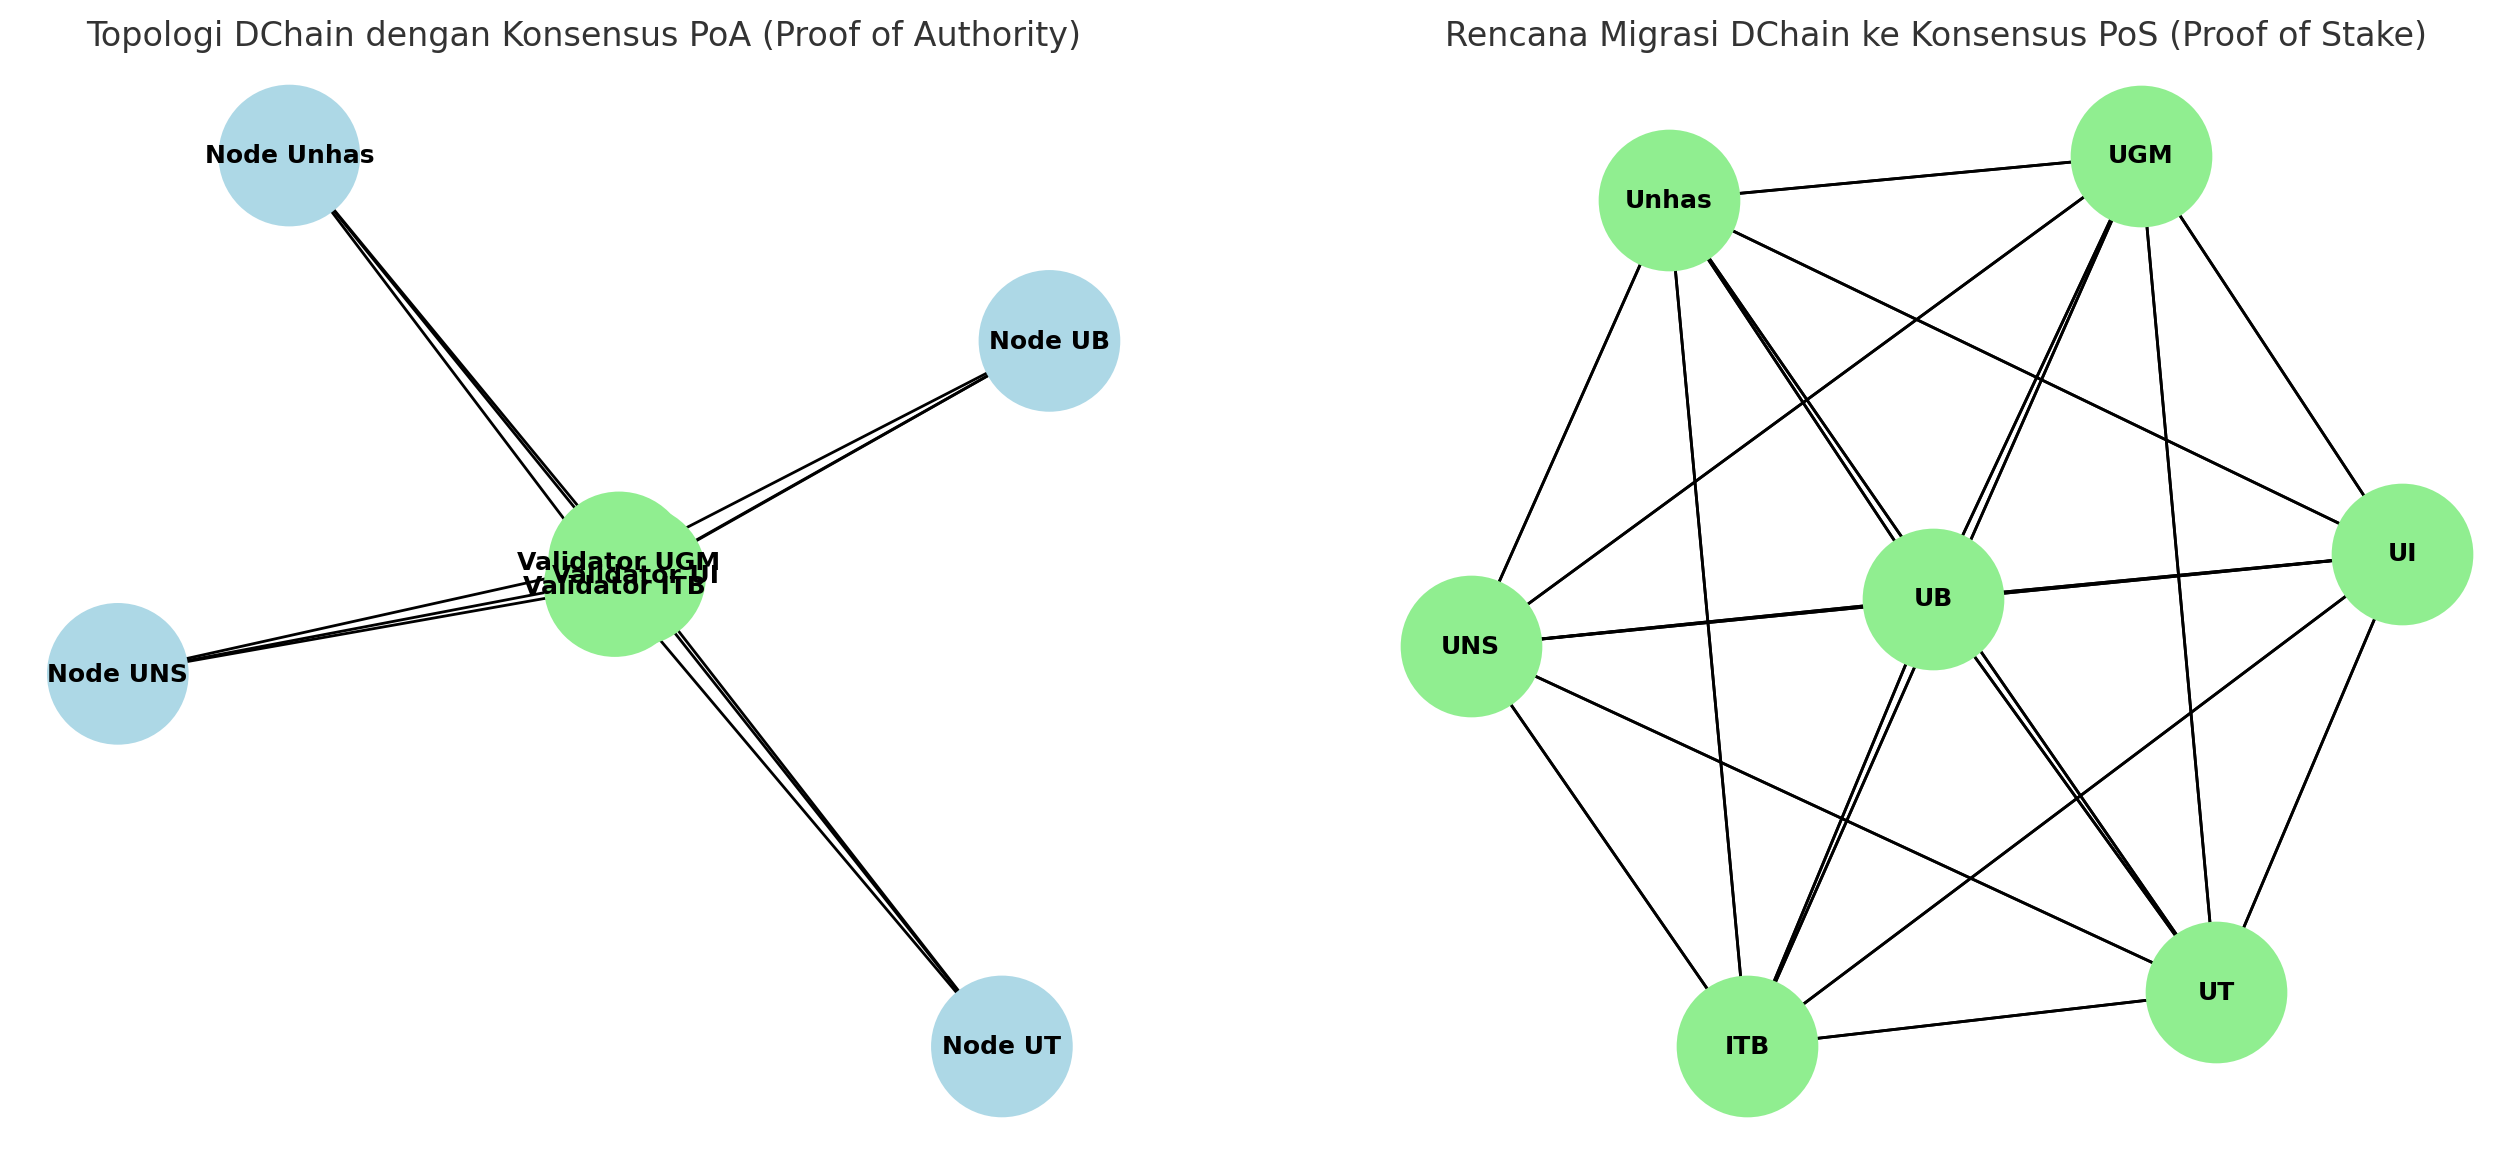
\includegraphics[width=\textwidth]{images/topology-dchain.png}
    \caption{Perbandingan topologi jaringan DChain pada mekanisme konsensus PoA dan PoS.}
    \label{fig:dchain_topologi}
\end{figure}

Gambar~\ref{fig:dchain_topologi} menggambarkan perbedaan topologi jaringan \textit{DChain} pada mekanisme konsensus \textit{Proof of Authority} (PoA) dan rencana migrasi ke \textit{Proof of Stake} (PoS). Pada arsitektur PoA, hanya sejumlah \textit{node} otoritatif yang memiliki kewenangan untuk memvalidasi transaksi dan menghasilkan blok baru, sementara \textit{node} lain berfungsi sebagai \textit{full node} untuk sinkronisasi data. Pola ini memberikan efisiensi dengan latensi rendah, tetapi tingkat desentralisasi terbatas karena proses validasi terpusat.

Sebaliknya, pada arsitektur PoS, setiap \textit{node} yang memiliki \textit{stake} dapat berpartisipasi sebagai validator, sehingga struktur jaringan menjadi lebih terdesentralisasi dan bersifat \textit{peer-to-peer}. Dengan mekanisme ini, proses validasi tidak lagi bergantung pada sejumlah \textit{node} tertentu, melainkan didistribusikan berdasarkan jumlah \textit{stake} yang dimiliki. Hal ini meningkatkan skalabilitas dan keamanan jaringan, meskipun berpotensi menambah latensi pada beban transaksi rendah.

\subsection{Proof of Authority (PoA)}

\textit{Proof of Authority} (PoA) merupakan salah satu mekanisme konsensus \textit{blockchain} yang menggunakan validator terbatas dan otoritatif untuk memverifikasi transaksi serta membentuk blok baru. Tidak seperti \textit{Proof of Work} (PoW) yang mengandalkan daya komputasi atau \textit{Proof of Stake} (PoS) yang didasarkan pada jumlah aset, PoA menitikberatkan pada identitas dan reputasi validator yang telah ditunjuk. Model ini menjadikan PoA sangat sesuai untuk \textit{blockchain} privat maupun konsorsium, termasuk aplikasi di sektor pendidikan seperti \textit{DChain}.

Dari sisi kelebihan, PoA memiliki beberapa keunggulan penting. Pertama, efisiensi transaksi yang tinggi karena mampu memproses ribuan transaksi per detik dengan latensi rendah, melampaui kinerja PoW maupun PoS \cite{reshi2025, joshi2021, chikezie2021}. Kedua, konsumsi energi rendah, sebab PoA tidak memerlukan daya komputasi besar untuk melakukan validasi blok, sehingga efisien bagi aplikasi dengan keterbatasan sumber daya \cite{reshi2025, joshi2021, sytnyk2024}. Ketiga, finalitas blok cepat, di mana transaksi segera dianggap sah karena validator telah diotorisasi sejak awal \cite{joshi2021, chikezie2021}.

Namun demikian, PoA juga memiliki sejumlah keterbatasan. Desentralisasi rendah menjadi kritik utama karena jumlah validator yang terbatas dapat menimbulkan risiko sentralisasi kekuasaan \cite{joshi2021, qiu2022}. Selain itu, terdapat potensi kolusi dan serangan internal jika validator bersepakat untuk bertindak jahat, sehingga integritas jaringan dapat terancam \cite{joshi2021, qiu2022}. PoA juga sangat bergantung pada reputasi dan kredibilitas validator, sehingga proses seleksi, pemantauan, dan rotasi validator menjadi aspek strategis yang menentukan keberlanjutan jaringan \cite{joshi2021, qiu2022}.

\begin{table}[ht]
\centering
\caption{Perbandingan Mekanisme Konsensus PoA, PoW, dan PoS}
\label{tab:perbandingan_konsensus}
\resizebox{\textwidth}{!}{
\begin{tabular}{|p{3cm}|p{3.5cm}|p{3.5cm}|p{3.5cm}|p{1.5cm}|}
\hline
\textbf{Aspek} & \textbf{Proof of Authority (PoA)} & \textbf{Proof of Work (PoW)} & \textbf{Proof of Stake (PoS)} & \textbf{Sumber} \\ \hline
Validator & Terbatas, berbasis otoritas/reputasi & Penambang dengan daya komputasi tinggi & Pemegang token yang dipilih berdasarkan jumlah kepemilikan & \cite{reshi2025, joshi2021, qiu2022} \\ \hline
Desentralisasi & Rendah – validator terbatas & Tinggi – siapa pun bisa menambang & Tinggi – siapa pun bisa berpartisipasi jika memiliki token & \cite{joshi2021, chikezie2021, qiu2022} \\ \hline
Efisiensi Energi & Sangat tinggi – tidak membutuhkan daya komputasi besar & Sangat rendah – boros energi karena mining & Sedang – lebih hemat energi dibanding PoW & \cite{reshi2025, joshi2021, sytnyk2024} \\ \hline
Kecepatan Transaksi & Sangat tinggi (latensi rendah, throughput tinggi) & Rendah – konfirmasi transaksi lambat & Sedang–tinggi – lebih cepat dari PoW, lebih lambat dari PoA & \cite{joshi2021, chikezie2021} \\ \hline
Finalitas Blok & Instan – blok langsung sah karena validator sudah diotorisasi & Probabilistik – membutuhkan beberapa konfirmasi blok & Relatif cepat – finalitas tercapai setelah validator menyetujui & \cite{joshi2021, chikezie2021, sytnyk2024} \\ \hline
Keamanan & Bergantung pada reputasi validator; rawan kolusi & Sangat tinggi, sulit diserang namun rentan 51\% attack & Tinggi, namun berisiko sentralisasi jika token terkonsentrasi & \cite{joshi2021, chikezie2021, qiu2022} \\ \hline
Risiko Sentralisasi & Tinggi – validator sedikit dan terpusat & Rendah – kompetisi terbuka & Sedang – bergantung pada distribusi token & \cite{joshi2021, qiu2022} \\ \hline
Kelebihan Utama & Efisiensi, kecepatan, konsumsi energi rendah, finalitas cepat & Keamanan tinggi, desentralisasi penuh, transparan & Hemat energi, mendukung skalabilitas, lebih adil & \cite{reshi2025, joshi2021, chikezie2021, sytnyk2024, qiu2022} \\ \hline
Keterbatasan Utama & Desentralisasi rendah, rawan kolusi, bergantung reputasi validator & Boros energi, lambat, biaya tinggi & Risiko sentralisasi aset, kompleksitas mekanisme & \cite{joshi2021, chikezie2021, qiu2022} \\ \hline
Cocok untuk & Blockchain privat, konsorsium, pendidikan, IoT & Blockchain publik, cryptocurrency (Bitcoin, Ethereum v1) & Blockchain publik modern, DeFi, NFT, platform berskala besar & \cite{joshi2021, chikezie2021, qiu2022} \\ \hline
\end{tabular}}
\end{table}

Tabel~\ref{tab:perbandingan_konsensus} menunjukkan bahwa dibandingkan PoW dan PoS, PoA unggul dalam efisiensi energi dan kecepatan transaksi, namun lemah dalam desentralisasi dan berpotensi menghadapi risiko sentralisasi.

Dalam konteks \textit{DChain}, mekanisme PoA digunakan dengan validator yang berasal dari universitas dan institusi pendidikan tinggi di Indonesia. Model ini mendukung efisiensi penerbitan serta verifikasi dokumen akademik seperti ijazah digital dengan kecepatan tinggi \cite{joshi2021, chikezie2021}. Meskipun demikian, meningkatnya jumlah pengguna \textit{DChain} menuntut adanya mekanisme pengawasan reputasi serta sistem rotasi validator untuk menjaga keamanan, transparansi, dan kepercayaan publik terhadap jaringan \cite{joshi2021, qiu2022}.

Dengan demikian, PoA terbukti efektif untuk \textit{blockchain} privat seperti \textit{DChain} karena efisiensi dan kecepatan yang ditawarkan, namun tetap membutuhkan perhatian terhadap aspek desentralisasi dan keamanan jangka panjang.


\subsection{Proof of Stake (PoS)}

\textit{Proof of Stake} (PoS) merupakan mekanisme konsensus \textit{blockchain} yang memilih validator berdasarkan jumlah aset atau \textit{stake} yang dimiliki dan dikunci dalam jaringan. Mekanisme ini hadir sebagai alternatif dari \textit{Proof of Work} (PoW) yang dikenal boros energi, dengan tujuan menghadirkan model validasi yang lebih efisien, hemat energi, dan berpotensi lebih desentralisasi \cite{zhang2025, li2023, feng2023}.

Salah satu keunggulan utama PoS adalah efisiensi energi yang jauh lebih baik dibandingkan PoW, karena tidak memerlukan proses \textit{mining} berbasis komputasi intensif. Hal ini menjadikan PoS lebih ramah lingkungan dan berkelanjutan \cite{zhang2025, li2023, wendl2022, mandal2023}. Selain itu, PoS dinilai mampu meningkatkan skalabilitas karena memungkinkan \textit{throughput} transaksi lebih tinggi dan latensi yang lebih rendah pada beban tinggi \cite{zhang2025, ge2022, li2020}. Dari sisi tata kelola jaringan, PoS juga berpotensi menghadirkan desentralisasi yang lebih luas jika didukung oleh desain insentif yang tepat, sehingga partisipasi validator dapat lebih inklusif \cite{li2023, nguyen2019}. Dari segi keamanan, biaya untuk melakukan serangan seperti \textit{51\% attack} menjadi sangat tinggi karena penyerang harus menguasai sebagian besar token yang beredar, sehingga PoS dipandang lebih aman dalam jangka panjang \cite{john2025, li2020}.

Namun, PoS tidak terlepas dari keterbatasan. Distribusi token yang tidak merata dapat menimbulkan risiko sentralisasi, karena pemegang token besar memiliki peluang lebih besar untuk menjadi validator dan memperoleh \textit{reward} \cite{zhao2023, li2023, nguyen2019}. PoS juga rentan terhadap serangan khas seperti \textit{nothing-at-stake} dan \textit{long-range attacks}, di mana validator dapat memvalidasi lebih dari satu cabang blok tanpa biaya tambahan \cite{deirmentzoglou2019, li2020, feng2023}. Dari sisi implementasi, keadilan distribusi \textit{reward} dan mekanisme insentif bagi validator kecil menjadi isu penting yang masih diperdebatkan \cite{li2023, nguyen2019}. Selain itu, migrasi dari konsensus lain ke PoS, misalnya dari PoA ke PoS, menuntut kompleksitas teknis yang tinggi serta penyesuaian parameter jaringan agar tetap stabil dan aman \cite{zhang2025, ge2022}.

Dalam konteks \textit{DChain}, rencana migrasi dari PoA ke PoS didorong oleh kebutuhan untuk meningkatkan desentralisasi, skalabilitas, dan keamanan jangka panjang. Meski demikian, migrasi ini juga membawa tantangan baru, antara lain pengaturan distribusi token, tata kelola insentif, serta potensi \textit{trade-off} antara efisiensi dan stabilitas. Oleh karena itu, pengujian komparatif performa PoA dan PoS menjadi langkah penting untuk menilai kelayakan PoS sebagai fondasi konsensus jangka panjang bagi \textit{DChain}.


\subsection{Algoritma Konsensus Spesifik}

Penelitian ini membandingkan dua implementasi spesifik dari keluarga konsensus PoA dan PoS, yaitu \textit{Clique} (standar Ethereum Geth PoA) dan \textit{Gasper} (standar Ethereum 2.0 PoS). Pemahaman mendalam tentang kedua protokol ini diperlukan untuk menginterpretasikan metrik \textit{finality} dan stabilitas.

\subsubsection{Clique (Proof of Authority)}
\textit{Clique} adalah protokol konsensus PoA yang digunakan secara luas pada jaringan uji (\textit{testnet}) Ethereum. Dalam Clique, node dibagi menjadi \textit{Signers} (validator terotorisasi) dan \textit{Non-Signers}. Clique menggunakan periode \textit{Epoch} (default 30.000 blok) untuk \textit{reset} hak \textit{voting} \textit{signers}, mencegah akumulasi data \textit{checkpoint} yang berlebihan \cite{eip225}. Blok diproduksi secara bergiliran (\textit{Round Robin}). Validator yang baru saja membuat blok tidak boleh membuat blok berikutnya segera (\textit{in-turn} vs \textit{out-of-turn}). Clique menawarkan \textit{Probabilistic Finality}. Secara teknis, reorganisasi rantai (\textit{reorg}) pendek dimungkinkan jika terjadi partisi jaringan, namun dalam kondisi normal dengan $N$ validator jujur, finalitas dianggap tercapai setelah $N/2 + 1$ blok \cite{eip225}.

\subsubsection{Gasper (Proof of Stake)}
\textit{Gasper} adalah protokol konsensus hibrida yang menggabungkan LMD-GHOST (\textit{Latest Message Driven Greediest Heaviest Observed Subtree}) sebagai aturan pemilihan cabang (\textit{fork choice rule}) dan Casper FFG (\textit{Friendly Finality Gadget}) sebagai mekanisme finalisasi \cite{buterin2020}. Waktu dibagi menjadi \textit{Slot} (12 detik) dan \textit{Epoch} (32 slot atau 6.4 menit). Setiap slot memiliki satu validator pengusul (\textit{proposer}) dan komite \textit{attester} yang memvoting validitas blok. Berbeda dengan PoW atau PoA Clique, Gasper memberikan \textit{Deterministic Finality}. Sebuah pasangan epoch dianggap \textit{Justified} jika mendapat 2/3 suara, dan \textit{Finalized} jika epoch berikutnya juga terjustifikasi. Transaksi pada blok yang \textit{Finalized} secara matematis tidak dapat dibatalkan tanpa membakar setidaknya 1/3 dari total ETH yang di-\textit{stake} \cite{saltini2021}.

\subsection{Benchmarking pada Blockchain}

\textit{Benchmarking} dalam konteks \textit{blockchain} merupakan proses sistematis untuk mengukur dan mengevaluasi kinerja jaringan terdistribusi melalui skenario eksperimen yang terkontrol. Tujuan utamanya adalah untuk menilai performa sistem, mengidentifikasi \textit{bottleneck}, serta membandingkan efektivitas mekanisme konsensus atau konfigurasi jaringan tertentu \cite{fan2020, dinh2017, thakkar2018}. Literatur umumnya membedakan dua pendekatan utama, yaitu \textit{micro-benchmarking}, yang berfokus pada metrik teknis spesifik seperti \textit{Transactions Per Second} (TPS), latensi, \textit{throughput}, dan penggunaan sumber daya; serta \textit{macro-benchmarking}, yang mengevaluasi kinerja keseluruhan sistem termasuk aspek skalabilitas, stabilitas, dan \textit{fault tolerance} \cite{dinh2017, nasrulin2022, gramoli2023}.

\subsubsection{Framework Benchmarking Blockchain}

Berbagai \textit{framework benchmarking} telah dikembangkan untuk mendukung penelitian dan pengujian performa \textit{blockchain}. \textit{Blockbench} merupakan salah satu framework awal yang digunakan untuk mengevaluasi \textit{private blockchain} melalui metrik \textit{throughput}, latensi, dan \textit{fault tolerance} \cite{dinh2017}. Framework lain seperti \textit{Hyperledger Caliper}, \textit{DLPS}, \textit{Gromit}, dan \textit{Diablo} memperluas cakupan pengujian dengan pendekatan modular dan ekstensibel, memungkinkan analisis lintas platform dan sistem konsensus \cite{fan2020, gramoli2023, sedlmeir2021}. 

Penggunaan \textit{workload generator} seperti \textit{Caliper}, serta \textit{monitoring tools} seperti \textit{Prometheus} dan \textit{Grafana}, kini menjadi praktik standar dalam eksperimen. Alat-alat ini berfungsi untuk menghasilkan beban transaksi terukur sekaligus merekam konsumsi sumber daya sistem (CPU, memori, dan I/O) secara real-time \cite{thakkar2018, nasrulin2022, ren2023}. Dengan kombinasi tersebut, pengujian dapat dilakukan secara terukur dan dapat direplikasi dalam berbagai konfigurasi jaringan.

\subsubsection{Tantangan dalam Benchmarking Blockchain}

Meskipun telah banyak kemajuan, benchmarking \textit{blockchain} tetap menghadapi sejumlah tantangan metodologis. Perbedaan konfigurasi eksperimen, heterogenitas platform \textit{blockchain}, serta ketiadaan metodologi standar sering kali menyulitkan replikasi hasil penelitian dan membatasi validitas perbandingan antar studi \cite{dinh2017, gramoli2023}. Selain itu, terdapat kesulitan dalam menyeimbangkan realisme \textit{workload} dengan kontrol eksperimen, yang dapat memengaruhi reliabilitas hasil \cite{thakkar2018, ren2023}.

\subsubsection{Praktik Terbaik dalam Benchmarking Blockchain}

Untuk mengatasi keterbatasan tersebut, penelitian terkini merekomendasikan sejumlah praktik terbaik, antara lain:
\begin{enumerate}[nolistsep]
    \item Penggunaan \textit{testbed} terbuka berbasis containerisasi seperti \textit{Docker} atau \textit{Kubernetes} untuk menjamin replikasi eksperimen.
    \item Standarisasi parameter uji, seperti TPS target, jumlah \textit{node}, waktu blok, dan jumlah \textit{worker}.
    \item Dokumentasi konfigurasi eksperimen secara transparan untuk meningkatkan validitas hasil.
    \item Replikasi eksperimen dengan variasi beban untuk menguji stabilitas dan \textit{fault tolerance}.
\end{enumerate}

Dengan penerapan prinsip-prinsip tersebut, benchmarking tidak hanya berfungsi sebagai alat evaluasi performa teknis, tetapi juga menjadi instrumen strategis dalam merancang, mengoptimalkan, dan memvalidasi efektivitas mekanisme konsensus \textit{blockchain} dalam aplikasi dunia nyata.


\subsection{Arsitektur Hyperledger Caliper}

\textit{Hyperledger Caliper} adalah alat \textit{benchmarking} \textit{blockchain} yang dikembangkan oleh Linux Foundation untuk mengukur kinerja spesifik dari berbagai implementasi \textit{blockchain} \cite{hyperledger_caliper}. Caliper dirancang dengan arsitektur modular yang memisahkan lapisan aplikasi uji (\textit{benchmark layer}) dari lapisan antarmuka \textit{blockchain} (\textit{adaptation layer}), memungkinkannya digunakan untuk berbagai platform seperti Ethereum (\textit{Besu}, \textit{Geth}) dan Hyperledger Fabric.

Arsitektur Caliper terdiri dari dua komponen proses utama:
\begin{itemize}[nolistsep]
    \item \textbf{Manager Process}: Bertindak sebagai orkestrator pusat yang membaca \textit{file} konfigurasi, menginisialisasi jaringan, dan membagi beban kerja kepada proses pekerja. \textit{Manager} juga bertanggung jawab untuk mengumpulkan hasil statistik dari pekerja dan menghasilkan laporan akhir \cite{kumar2020}.
    \item \textbf{Worker Process}: Proses independen yang bertugas mengeksekusi beban kerja (\textit{workload}). Masing-masing \textit{worker} menjalankan \textit{loop} transaksi secara mandiri. Penggunaan banyak \textit{worker} memungkinkan simulasi konkurensi klien, di mana \textit{throughput} total sistem dihitung dari agregasi \textit{output} seluruh \textit{worker} \cite{kumar2020}.
\end{itemize}

Pentingnya fitur \textit{Worker Scaling} dalam Caliper terletak pada hukum Amdahl: jika pembangkitan beban dilakukan oleh satu proses, maka CPU klien sering kali menjadi \textit{bottleneck} sebelum kapasitas jaringan \textit{blockchain} tercapai. Dengan mendistribusikan beban ke \textit{multi-worker}, Caliper dapat membanjiri jaringan hingga titik jenuh, memastikan validitas pengukuran kapasitas maksimum \cite{hyperledger_caliper, nasir2022}.

\subsection{Observabilitas Sistem Terdistribusi}

Dalam pengelolaan sistem terdistribusi kompleks seperti \textit{blockchain}, pendekatan observabilitas melampaui \textit{monitoring} tradisional. Jika \textit{monitoring} menjawab pertanyaan "apakah sistem sehat?", observabilitas menjawab "mengapa sistem tidak sehat?" dengan menganalisis \textit{output} eksternal sistem \cite{picco2021}. Tiga pilar utama observabilitas adalah \textit{Metrics}, \textit{Logs}, dan \textit{Traces}. Penelitian ini secara spesifik berfokus pada pilar \textit{Metrics} untuk analisis performa kuantitatif.

Untuk menangkap dinamika performa \textit{blockchain} yang berubah cepat, digunakan \textit{Time-Series Database} (TSDB) seperti Prometheus. Berbeda dengan \textit{database} relasional yang dioptimalkan untuk integritas transaksional, TSDB dioptimalkan untuk penulisan data berkecepatan tinggi dan kueri berbasis rentang waktu \cite{prometheus_docs}. Prometheus bekerja dengan mekanisme \textit{scraping}, di mana server secara periodik menarik data dari target melalui protokol HTTP \cite{prometheus_docs}. Grafana berperan sebagai lapisan visualisasi yang mengubah data mentah dari TSDB menjadi dasbor interaktif, memungkinkan analisis korelasi data \cite{chakravarthy2019}.

\subsection{Virtualisasi Berbasis Kontainer}

Infrastruktur penelitian ini dibangun di atas teknologi virtualisasi berbasis kontainer, yang menawarkan pendekatan lebih ringan dibandingkan mesin virtual (VM) tradisional. Kontainer mengemas aplikasi beserta seluruh dependensinya dalam satu unit terisolasi yang berjalan di atas kernel OS \textit{host} yang sama. Hal ini menghilangkan \textit{overhead} sistem operasi tamu yang ada pada VM, memungkinkan efisiensi sumber daya yang jauh lebih tinggi \cite{bernstein2014}.

Untuk mengelola siklus hidup kontainer di banyak \textit{host}, digunakan \textit{Kubernetes}, khususnya distribusi K3s yang ringan \cite{k3s_io}. Unit eksekusi terkecil adalah \textit{Pod}, yang membungkus satu atau lebih kontainer. Dalam arsitektur konsensus PoS, pola \textit{sidecar} sering digunakan, di mana kontainer klien eksekusi (Geth) dan klien konsensus (Prysm) berjalan dalam satu \textit{Pod} untuk komunikasi \textit{low-latency} \cite{singh2020}.

\subsection{Metrik dan Konsep Evaluasi Performa}

Evaluasi kinerja \textit{blockchain} memerlukan pemahaman mendalam tentang berbagai metrik dan fenomena unik. Berikut adalah terminologi teknis yang digunakan:

\begin{enumerate}
    \item \textbf{Knee Point}: Titik kritis dalam kurva kinerja di mana sistem mencapai kapasitas pemrosesan maksimumnya. Setelah titik ini, penambahan beban menyebabkan lonjakan drastis pada latensi \cite{avritzer2020}.
    \item \textbf{Hockey Stick Curve}: Pola grafik hubungan antara beban (TPS) dan latensi. Pada beban rendah, latensi stabil (seluncuran hoki), namun meningkat eksponensial saat mendekati kapasitas maksimum (gagang hoki) \cite{gregg2020}.
    \item \textbf{Soak Test}: Pengujian durabilitas untuk memvalidasi stabilitas sistem dalam jangka panjang, mendeteksi masalah seperti kebocoran memori \cite{hyperledger_caliper}.
    \item \textbf{Coefficient of Variation (CV)}: Ukuran statistik untuk mengevaluasi konsistensi \textit{throughput}. Nilai CV rendah menunjukkan performa stabil \cite{jain1991}.
    \item \textbf{Steady State vs Cold Start}: \textit{Steady State} adalah fase di mana sistem berjalan stabil, sedangkan \textit{Cold Start} adalah fase inisialisasi yang sering kali bias \cite{spec2021}.
    \item \textbf{Sub-linear Scaling}: Fenomena di mana penambahan sumber daya tidak menghasilkan peningkatan performa yang sebanding karena adanya bagian proses yang sekuensial (Hukum Amdahl) \cite{amdahl1967}.
\end{enumerate}

\subsection{Faktor yang Mempengaruhi Performa Blockchain}

Performa \textit{blockchain} sangat dipengaruhi oleh konfigurasi teknis dan lingkungan operasional jaringan. Faktor-faktor seperti jumlah \textit{node} validator, waktu blok, ukuran blok, beban transaksi, konfigurasi \textit{workload generator}, jenis transaksi, serta spesifikasi infrastruktur terbukti memiliki dampak signifikan terhadap metrik utama, yaitu \textit{throughput}, latensi, konsumsi sumber daya, dan stabilitas jaringan \cite{kaur2021, hao2018, shahsavari2022, xu2021, gobel2017}.

Jumlah \textit{node} validator berkorelasi dengan tingkat desentralisasi dan keamanan, tetapi sekaligus menambah \textit{overhead} komunikasi yang dapat menurunkan \textit{throughput} ketika jumlah validator meningkat \cite{kaur2021, hao2018}. Waktu blok (\textit{block time}) berperan penting dalam menentukan latensi transaksi. Interval yang lebih pendek memangkas waktu konfirmasi, namun dapat meningkatkan risiko instabilitas jaringan \cite{shahsavari2022, xu2021}. Ukuran blok (\textit{block size}) memungkinkan pemrosesan transaksi dalam jumlah lebih besar per blok, tetapi dapat memicu keterlambatan propagasi data dan meningkatkan frekuensi \textit{fork} \cite{shahsavari2022, gobel2017}.

Selain itu, beban transaksi (\textit{transaction load}) serta jumlah \textit{worker} dalam \textit{workload generator} seperti \textit{Hyperledger Caliper} sangat menentukan hasil \textit{benchmarking}. \textit{Throughput} umumnya meningkat seiring kenaikan beban hingga titik jenuh, setelah itu latensi meningkat secara drastis \cite{thakkar2018, ucbas2023}. Faktor lain yang turut memengaruhi adalah jenis transaksi: operasi tulis cenderung lebih berat pada I/O, sedangkan transaksi komputasi intensif mengonsumsi CPU lebih besar \cite{dinh2017, gaba2022}.

Dari sisi infrastruktur, spesifikasi CPU, memori, \textit{bandwidth} jaringan, serta penggunaan \textit{containerization} (Docker) dan \textit{orchestration} (Kubernetes) terbukti berpengaruh terhadap efisiensi \textit{deployment} serta skalabilitas sistem \cite{zheng2019, wu2022}. Penelitian juga menunjukkan adanya interaksi antar faktor, misalnya kombinasi waktu blok singkat dengan ukuran blok besar dapat meningkatkan \textit{throughput}, tetapi dengan \textit{trade-off} berupa menurunnya konsistensi jaringan \cite{shahsavari2022, gobel2017}. Oleh karena itu, pengaturan parameter secara sistematis melalui eksperimen \textit{benchmarking} sangat penting agar hasil evaluasi performa valid, representatif, dan dapat direplikasi \cite{kaur2021, thakkar2018, fan2020}.

\begin{table}[ht]
\centering
\caption{Faktor Teknis yang Mempengaruhi Performa Blockchain}
\label{tab:faktor_performa}
\resizebox{\textwidth}{!}{
\begin{tabular}{|p{3.5cm}|p{5cm}|p{5cm}|p{2cm}|}
\hline
\textbf{Faktor} & \textbf{Dampak Utama} & \textbf{Trade-off} & \textbf{Sumber} \\ \hline
Jumlah Node Validator & Meningkatkan desentralisasi dan keamanan; menambah redundansi jaringan & Menurunkan throughput karena overhead komunikasi meningkat & \cite{kaur2021, hao2018} \\ \hline
Waktu Blok (Block Time) & Interval pendek menurunkan latensi dan mempercepat konfirmasi transaksi & Risiko instabilitas jaringan dan meningkatnya frekuensi fork & \cite{shahsavari2022, xu2021} \\ \hline
Ukuran Blok (Block Size) & Blok lebih besar menampung lebih banyak transaksi, throughput meningkat & Propagasi lebih lambat, risiko fork lebih tinggi & \cite{shahsavari2022, gobel2017} \\ \hline
Beban Transaksi (Load) & Throughput meningkat seiring beban, hingga titik jenuh & Setelah batas, latensi meningkat drastis, sistem jadi tidak stabil & \cite{thakkar2018, ucbas2023} \\ \hline
Jumlah Worker (Caliper) & Paralelisme transaksi meningkat, simulasi beban lebih realistis & Terlalu banyak worker dapat memicu overload dan bottleneck & \cite{thakkar2018, ucbas2023} \\ \hline
Jenis Transaksi & Operasi baca lebih ringan; tulis dan komputasi intensif menambah konsumsi CPU/I/O & Beban tinggi pada operasi tulis/komputasi menurunkan throughput & \cite{dinh2017, gaba2022} \\ \hline
Infrastruktur (VPS/OS) & CPU, RAM, bandwidth, dan containerization memengaruhi efisiensi dan skalabilitas & Infrastruktur lemah menyebabkan bottleneck; konfigurasi salah menurunkan validitas eksperimen & \cite{zheng2019, wu2022} \\ \hline
\end{tabular}}
\end{table}

Tabel~\ref{tab:faktor_performa} merangkum hubungan antara faktor-faktor teknis, dampaknya terhadap performa \textit{blockchain}, serta \textit{trade-off} yang harus dipertimbangkan dalam desain eksperimen maupun implementasi nyata. Visualisasi ini menunjukkan bahwa setiap parameter memiliki konsekuensi ganda: satu sisi memberikan peningkatan performa, sementara di sisi lain dapat menimbulkan keterbatasan. Oleh karena itu, pendekatan \textit{benchmarking} yang sistematis diperlukan untuk menyeimbangkan parameter-parameter tersebut agar hasil evaluasi valid, representatif, dan relevan terhadap konteks aplikasi seperti jaringan \textit{DChain}.

Dengan demikian, pemahaman atas faktor-faktor teknis ini tidak hanya mendukung optimasi performa \textit{blockchain}, tetapi juga membantu menentukan konfigurasi yang sesuai dengan kebutuhan spesifik, terutama dalam konteks penelitian perbandingan mekanisme konsensus PoA dan PoS pada \textit{DChain}.


\subsection{Hubungan dengan Penelitian Ini}

Penelitian ini merupakan turunan langsung dari berbagai riset terdahulu yang membandingkan performa mekanisme konsensus \textit{Proof of Authority} (PoA) dan \textit{Proof of Stake} (PoS). Sebagaimana telah dibahas pada Bab 2.1 Tinjauan Pustaka, literatur sebelumnya banyak mengkaji performa kedua konsensus tersebut dengan menggunakan metrik \textit{benchmarking} utama seperti \textit{throughput} (TPS) dan latensi. Selain itu, teori mengenai karakteristik PoA dan PoS, serta metodologi \textit{benchmarking} dengan alat seperti \textit{Hyperledger Caliper}, menjadi fondasi penting bagi penelitian ini \cite{dinh2017, fan2020, thakkar2018, nguyen2019, li2023}.

Meskipun demikian, riset terdahulu masih memiliki sejumlah keterbatasan. Sebagian besar studi hanya menitikberatkan pada pengujian performa dasar dengan parameter terbatas, sehingga belum mencakup aspek lain yang juga krusial seperti penggunaan sumber daya (CPU, memori, dan disk) maupun stabilitas sistem dalam menghadapi variasi beban dan konfigurasi jaringan \cite{kaur2021, ucbas2023, gramoli2023}. Keterbatasan ini menyebabkan hasil penelitian sebelumnya cenderung bersifat parsial dan sulit digeneralisasi untuk konteks implementasi yang lebih luas, khususnya pada platform berskala nasional.

Penelitian ini hadir untuk mengisi kesenjangan tersebut dengan tiga kontribusi utama. Pertama, cakupan variabel uji diperluas dengan menambahkan \textit{resource usage} dan stabilitas sistem sebagai metrik baru di samping TPS dan latensi. Kedua, penelitian ini secara khusus difokuskan pada \textit{DChain}, yaitu infrastruktur \textit{blockchain} nasional untuk pendidikan tinggi di Indonesia, sehingga relevansi hasilnya lebih kontekstual dan strategis. Ketiga, eksperimen dilakukan dengan \textit{multi-skenario benchmarking} yang lebih komprehensif, mencakup variasi beban transaksi (\textit{transaction load}), jumlah \textit{node} validator, waktu blok (\textit{block time}), serta jumlah \textit{worker} pada \textit{Caliper}.

Dengan pendekatan ini, penelitian diharapkan tidak hanya memperkuat temuan literatur terdahulu, tetapi juga memberikan landasan empiris yang lebih menyeluruh untuk mendukung pengambilan keputusan terkait migrasi konsensus dari PoA ke PoS pada jaringan \textit{DChain}.


\section{Analisis Perbandingan Metode}

\subsection{Metode Penelitian Terdahulu}

Penelitian performa \textit{blockchain} telah menggunakan berbagai pendekatan metodologis, mulai dari studi literatur, simulasi matematis, hingga eksperimen nyata. Setiap metode memiliki keunggulan dan keterbatasan dalam merepresentasikan kinerja jaringan \textit{blockchain}.

Pendekatan studi literatur dan survei banyak digunakan untuk merangkum teori, perkembangan teknologi, serta tantangan utama \textit{blockchain}, khususnya dalam aspek keamanan, desentralisasi, dan mekanisme konsensus. Namun, metode ini cenderung bersifat konseptual dan tidak menghasilkan data empiris langsung terkait performa jaringan \cite{fan2020, dabbagh2021, bamakan2020}.

Pendekatan simulasi berbasis model matematis juga banyak digunakan, misalnya dengan memanfaatkan teori antrian atau model graf untuk mengevaluasi pengaruh parameter teknis seperti ukuran blok, waktu blok, dan jumlah \textit{node} terhadap \textit{throughput} maupun latensi. Keunggulannya adalah fleksibilitas dan biaya rendah, tetapi keterbatasannya terletak pada representasi yang sering kali terlalu sederhana sehingga tidak sepenuhnya mencerminkan kompleksitas sistem \textit{blockchain} nyata \cite{xu2021, zhou2020, shahsavari2022, huang2018}.

Pendekatan yang semakin dominan adalah eksperimen nyata melalui \textit{benchmarking}, di mana peneliti membangun jaringan uji (\textit{testnet}) menggunakan \textit{framework} seperti \textit{Blockbench} atau \textit{Hyperledger Caliper} untuk mengukur metrik performa seperti \textit{Transactions Per Second} (TPS), latensi, penggunaan sumber daya, skalabilitas, dan stabilitas \cite{dinh2017, esmaili2024, abreu2022, misra2021}. Studi-studi tersebut dianggap lebih representatif karena langsung memodelkan kondisi implementasi \textit{blockchain} nyata.

Sebagai contoh, penelitian oleh Palguno Wicaksono dkk. \cite{wicaksono2021} melakukan eksperimen performa pada jaringan Ethereum privat untuk membandingkan mekanisme konsensus PoA dan PoS. Namun, pengujian mereka masih terbatas pada metrik TPS dan latensi, tanpa mempertimbangkan penggunaan sumber daya maupun stabilitas jaringan. Hal ini menunjukkan adanya ruang penelitian lanjutan untuk memperluas metrik evaluasi agar lebih komprehensif.

Jika dibandingkan dengan penelitian sebelumnya, desain eksperimen dalam penelitian ini lebih komprehensif karena melibatkan variabel tambahan seperti jumlah \textit{node}, waktu blok (\textit{block time}), jumlah \textit{worker}, serta jenis transaksi. Selain itu, fokus penelitian diarahkan pada \textit{DChain} sebagai platform \textit{blockchain} nasional, sehingga hasilnya memiliki relevansi kontekstual yang tinggi. Dengan demikian, penelitian ini tidak hanya mengadopsi pendekatan \textit{benchmarking} yang telah terbukti relevan, tetapi juga memperluas cakupan pengujian untuk mengisi kekosongan yang masih ada dalam penelitian terdahulu.


\subsection{Kelebihan dan Kekurangan Berbagai Metode}

Penelitian mengenai performa \textit{blockchain} secara umum menggunakan tiga pendekatan utama, yaitu studi literatur atau survei, simulasi atau model matematis, dan eksperimen atau \textit{benchmarking} nyata. Setiap metodologi memiliki keunggulan sekaligus keterbatasan dalam menggambarkan karakteristik performa sistem \textit{blockchain}.

Studi literatur atau survei banyak digunakan untuk memetakan perkembangan teknologi, teori konsensus, serta tantangan yang ada dalam riset \textit{blockchain}. Pendekatan ini, seperti \textit{systematic literature review} (SLR) dan \textit{bibliometric analysis}, memungkinkan pemahaman yang cepat, menyeluruh, dan hemat biaya terhadap tren riset. Namun, karena bersifat konseptual, metode ini tidak dapat memberikan data empiris langsung mengenai performa aktual \textit{blockchain} \cite{fan2020, rico2023, bellucci2022, zheng2019}.

Simulasi berbasis model matematis menjadi pendekatan lain yang banyak dipakai untuk menilai dampak parameter teknis seperti ukuran blok, waktu blok, atau jumlah \textit{node} terhadap performa jaringan. Contohnya adalah penggunaan model antrian Poisson, simulasi Monte Carlo, maupun \textit{Markov chains}. Metode ini relatif murah dan fleksibel karena memungkinkan pengujian banyak parameter sekaligus. Akan tetapi, hasil simulasi sering kali tidak sepenuhnya mencerminkan kondisi nyata karena banyaknya asumsi penyederhanaan yang digunakan \cite{fan2020, bellucci2022, cao2021}.

Eksperimen nyata atau \textit{benchmarking} dinilai sebagai pendekatan paling representatif dalam mengevaluasi performa \textit{blockchain}. Dengan memanfaatkan \textit{framework} seperti \textit{Blockbench} atau \textit{Hyperledger Caliper}, penelitian dapat menghasilkan data empiris terkait metrik utama seperti \textit{throughput}, latensi, \textit{scalability}, dan \textit{fault tolerance}. Pendekatan ini memberikan hasil yang lebih realistis dan relevan terhadap implementasi \textit{blockchain} di dunia nyata. Namun, keterbatasannya terletak pada kebutuhan sumber daya yang lebih besar, baik dari sisi infrastruktur, waktu, maupun biaya. Selain itu, eksperimen nyata cenderung lebih kompleks karena variabel lingkungan sering sulit dikendalikan sepenuhnya \cite{fan2020, cao2021}.

Berdasarkan analisis tersebut, dapat disimpulkan bahwa tidak ada satu metode yang sempurna untuk mengevaluasi performa \textit{blockchain}. Meski demikian, metode eksperimen dipilih dalam penelitian ini karena mampu memberikan data empiris yang paling sesuai untuk menjawab rumusan masalah, khususnya dalam mengevaluasi efisiensi dan efektivitas konsensus \textit{Proof of Authority} (PoA) dan \textit{Proof of Stake} (PoS) di jaringan \textit{DChain}.

\begin{table}[H]
\centering
\caption{Perbandingan Kelebihan dan Kekurangan Berbagai Metode Evaluasi Blockchain}
\label{tab:metode_perbandingan}
\resizebox{\textwidth}{!}{
\begin{tabular}{|p{3.5cm}|p{5cm}|p{5cm}|p{2cm}|}
\hline
\textbf{Metode Penelitian} & \textbf{Kelebihan Utama} & \textbf{Kekurangan Utama} & \textbf{Sumber} \\ \hline
Studi Literatur / Survei & Komprehensif, cepat, biaya rendah, memberikan gambaran teori dan tren riset & Tidak menghasilkan data empiris; sulit menilai performa aktual & \cite{fan2020, rico2023, bellucci2022, zheng2019} \\ \hline
Simulasi / Model Matematis & Fleksibel, murah, memungkinkan analisis parameter teknis kompleks & Banyak asumsi penyederhanaan, hasil kurang realistis terhadap kondisi implementasi nyata & \cite{fan2020, bellucci2022, cao2021} \\ \hline
Eksperimen / Benchmarking Nyata & Memberikan data empiris; hasil lebih representatif dan kontekstual terhadap implementasi \textit{blockchain} & Membutuhkan sumber daya besar (waktu, biaya, infrastruktur); kompleksitas tinggi & \cite{fan2020, cao2021} \\ \hline
\end{tabular}}
\end{table}

Tabel~\ref{tab:metode_perbandingan} merangkum perbandingan antara ketiga metode utama yang digunakan dalam penelitian performa \textit{blockchain}. Berdasarkan pertimbangan empiris dan relevansi, pendekatan eksperimen dipilih karena paling sesuai untuk menilai efektivitas mekanisme konsensus \textit{PoA} dan \textit{PoS} pada jaringan \textit{DChain}.


\subsection{Alasan Pemilihan Metode Eksperimen dalam Penelitian Ini}

Penelitian ini secara sadar memilih metode eksperimen (\textit{benchmarking} nyata) dibandingkan studi literatur atau simulasi. Pendekatan literatur, seperti \textit{systematic review} atau \textit{bibliometric analysis}, memang bermanfaat untuk memetakan teori dan tren penelitian \textit{blockchain}, tetapi tidak mampu memberikan bukti kuantitatif terkait performa aktual jaringan \cite{fan2020, rico2023}. Sementara itu, simulasi berbasis model matematis, seperti antrian Poisson atau simulasi Monte Carlo, menawarkan fleksibilitas dan biaya rendah untuk mengevaluasi parameter teknis, namun sering kali terlalu menyederhanakan kompleksitas sistem nyata sehingga hasilnya kurang representatif \cite{zhou2020, shahsavari2022}.

Sebaliknya, \textit{benchmarking} eksperimental memungkinkan pengukuran langsung terhadap metrik performa inti \textit{blockchain}, termasuk \textit{Transactions Per Second} (TPS), latensi, penggunaan sumber daya, skalabilitas, dan stabilitas. Metrik ini bersifat objektif, dapat diukur, serta mencerminkan efisiensi dan efektivitas mekanisme konsensus dalam kondisi operasional yang menyerupai implementasi nyata \cite{dinh2017, zheng2019}.

Selain itu, fokus penelitian ini adalah pada perbandingan \textit{Proof of Authority} (PoA) dan \textit{Proof of Stake} (PoS), sejalan dengan \textit{roadmap} DChain yang memang dirancang untuk bermigrasi dari PoA ke PoS. Konsensus lain seperti PBFT atau DPoS, meskipun menarik secara akademis, tidak relevan secara praktis karena tidak digunakan dalam implementasi DChain \cite{lashkari2021, zhang2020}. Oleh karena itu, pengujian empiris berbasis eksperimen dipandang sebagai metode yang paling tepat untuk mengisi \textit{gap} penelitian terdahulu yang umumnya hanya mengukur TPS dan latensi, tanpa mencakup penggunaan sumber daya dan stabilitas jaringan \cite{wicaksono2022}.

Dengan demikian, metode eksperimen dipilih bukan hanya karena memberikan hasil yang paling representatif, tetapi juga karena merupakan satu-satunya pendekatan yang \textit{feasible} untuk menjawab rumusan masalah penelitian ini.


\subsection{Kriteria Evaluasi Alat Benchmarking}

\textit{Benchmarking} merupakan aspek penting dalam evaluasi performa \textit{blockchain} karena mampu memberikan data empiris yang terukur mengenai \textit{throughput}, \textit{latency}, \textit{resource usage}, \textit{scalability}, dan stabilitas konsensus. Untuk menghasilkan evaluasi yang kredibel, alat \textit{benchmarking} harus memenuhi sejumlah kriteria fundamental. Literatur menekankan bahwa dukungan multi-metrik, variasi \textit{workload}, integrasi \textit{monitoring}, \textit{reproducibility}, dan portabilitas merupakan dimensi utama dalam menilai kualitas sebuah alat \textit{benchmarking} \cite{fan2020, beyer2017, martinez2022}.

Pertama, dukungan multi-metrik sangat penting, karena performa \textit{blockchain} tidak dapat direduksi hanya pada satu indikator seperti TPS. Alat yang baik harus mampu menangkap metrik komprehensif, termasuk \textit{latency}, konsumsi CPU/RAM, utilisasi \textit{bandwidth}, hingga konsumsi energi \cite{fan2020, zheng2019}. Kedua, variasi \textit{workload} memungkinkan evaluasi pada skenario berbeda, baik sintetis maupun realistis (misalnya transaksi token, kontrak pintar, atau simulasi IoT) \cite{dinh2017, beyer2017}. Ketiga, \textit{reproducibility} dan dokumentasi yang jelas merupakan kunci agar hasil eksperimen dapat diverifikasi dan diulang oleh peneliti lain \cite{beyer2017, beyer2024}. Keempat, portabilitas dan aksesibilitas—misalnya melalui \textit{Docker} atau \textit{Kubernetes}—menjadi nilai tambah agar eksperimen dapat dijalankan di berbagai lingkungan tanpa konfigurasi kompleks \cite{martinez2022, quetschlich2022}. Terakhir, pemeliharaan aktif dan dukungan komunitas penting untuk memastikan alat tetap relevan mengikuti perkembangan teknologi \textit{blockchain} \cite{zheng2019}.

Berdasarkan analisis literatur, dapat diidentifikasi perbedaan karakteristik antara beberapa \textit{framework} populer yang digunakan untuk \textit{benchmarking blockchain}. \textit{Hyperledger Caliper} menonjol karena bersifat \textit{open-source}, modular, mendukung berbagai platform (\textit{Ethereum}, \textit{Fabric}, \textit{Besu}, \textit{Quorum}), serta terintegrasi dengan \textit{monitoring tools} seperti \textit{Prometheus} dan \textit{Grafana} \cite{fan2020, zheng2019}. \textit{Blockbench} lebih berfokus pada \textit{private blockchain} seperti \textit{Hyperledger Fabric} dan \textit{Ethereum privat}, dengan kekuatan pada \textit{micro-benchmarking} komponen spesifik, meskipun dokumentasi dan pembaruan sudah jarang dilakukan sejak 2022 \cite{dinh2017}. \textit{PERSECUS} dan \textit{Diablo} menonjol pada aspek \textit{reproducibility} dengan dukungan \textit{workload generator} realistis, sementara \textit{Gromit} dan \textit{BlockCompass} mengarah ke \textit{macro-benchmarking} sistem utuh lintas platform \cite{beyer2024, martinez2022}.

\begin{table}[H]
\centering
\caption{Perbandingan Alat Benchmarking Blockchain}
\label{tab:benchmarking_comparison}
\resizebox{\textwidth}{!}{
\begin{tabular}{|p{2.8cm}|p{3.5cm}|p{3cm}|p{4cm}|p{4cm}|}
\hline
\textbf{Alat} & \textbf{Metrik Utama} & \textbf{Platform Didukung} & \textbf{Kelebihan} & \textbf{Keterbatasan} \\ \hline
\textbf{Hyperledger Caliper} & TPS, latency, resource usage, scalability, stability & Ethereum, Fabric, Besu, Quorum & \textit{Open-source}, modular, integrasi \textit{Prometheus/Grafana}, aktif dipelihara & Instalasi kompleks, kurva belajar tinggi \\ \hline
\textbf{Blockbench} & Throughput, latency, scalability, fault tolerance & Ethereum (geth), Parity, Fabric & \textit{Framework} komprehensif, cocok untuk \textit{private blockchain} & Tidak aktif dikembangkan, \textit{workload} terbatas \\ \hline
\textbf{PERSECUS} & TPS, latency, CPU/RAM, gas, energi & Ethereum, Fabric & Fokus pada \textit{reproducibility}, \textit{stress testing} modular & Dokumentasi publik minim \\ \hline
\textbf{Diablo} & Latency, gas cost, error resilience & Ethereum, Fabric, Tendermint & Kuat dalam skenario \textit{fault injection}, \textit{workload} scripting fleksibel & Masih tahap pengembangan awal \\ \hline
\textbf{Gromit} & Throughput, storage overhead, metadata cost & Ethereum, Fabric & Analisis makro lintas platform, fokus metadata & Komunitas kecil, kurang populer \\ \hline
\textbf{BlockCompass} & Throughput, resource efficiency & Enterprise Blockchain & Integrasi \textit{enterprise}, dukungan \textit{workload} realistis & Tidak \textit{open-source}, akses terbatas \\ \hline
\textbf{Grafana + Prometheus} & CPU, RAM, bandwidth (monitoring eksternal) & Agnostik (umum) & Visualisasi kuat, fleksibel lintas platform & Tidak menghasilkan \textit{workload}, hanya \textit{monitoring} \\ \hline
\end{tabular}}
\end{table}

Tabel~\ref{tab:benchmarking_comparison} menunjukkan bahwa \textit{Hyperledger Caliper} memenuhi hampir semua kriteria evaluasi alat \textit{benchmarking}: mendukung multi-metrik, variasi \textit{workload}, integrasi \textit{monitoring}, \textit{reproducibility} melalui containerization, serta pemeliharaan aktif \cite{fan2020, martinez2022, zheng2019}. Selain itu, Caliper telah banyak digunakan dalam penelitian empiris untuk mengevaluasi performa konsensus PoA dan PoS pada platform \textit{Ethereum} dan turunannya, termasuk \textit{DChain}. Oleh karena itu, pemilihan \textit{Hyperledger Caliper} dalam penelitian ini dinilai paling sesuai secara ilmiah dan praktis dibandingkan dengan alat lain yang tersedia.


\subsection{Perbandingan Desain dan Skenario Eksperimen dengan Penelitian Terdahulu}

Riset \textit{benchmarking blockchain} telah mengalami perkembangan signifikan dari eksperimen sederhana menuju \textit{framework} yang lebih komprehensif, dengan fokus pada penggunaan multi-metrik dan skenario uji yang beragam. Pada tahap awal, beberapa penelitian cenderung terbatas dalam desain eksperimen. Misalnya, Wicaksono \textit{dkk.} hanya menggunakan satu \textit{worker} serta menguji metrik dasar berupa \textit{throughput} (TPS) dan \textit{latency}, tanpa mempertimbangkan parameter lain yang dapat memengaruhi performa sistem. Studi lain oleh Choi dan Hong \cite{choi2020}, serta Arslan \textit{dkk.} \cite{arslan2020}, lebih berfokus pada jaringan Ethereum privat dengan beban sederhana, sehingga hasilnya masih jauh dari gambaran performa komprehensif dalam kondisi nyata.

Perkembangan lebih lanjut ditunjukkan oleh munculnya \textit{framework benchmarking} generik seperti Blockchain Benchmarking Framework (BBF), BCTMark, BlockCompass, dan Diablo yang memungkinkan pengujian lintas platform (\textit{Ethereum}, \textit{Hyperledger}, \textit{Quorum}, dll.) dengan konfigurasi parameter yang lebih luas, termasuk simulasi serangan, \textit{node failure}, dan \textit{workload} dinamis \cite{touloupou2024, saingre2020, rasolroveicy2024, lebedev2024}. Studi-studi terbaru juga mulai mengadopsi multi-metrik, tidak hanya mengukur \textit{throughput} dan \textit{latency}, tetapi juga \textit{resource usage} (CPU, RAM, \textit{bandwidth}), \textit{scalability}, \textit{fault tolerance}, dan bahkan konsumsi energi \cite{fan2020, pradhan2022, li2024, chacko2023}. Beberapa penelitian menggunakan pendekatan simulasi atau eksperimen independen untuk mengevaluasi dampak parameter tertentu, seperti \textit{network delay}, beban IoT, hingga aplikasi pada \textit{supply chain} dan kesehatan \cite{chen2021, longo2019, purusottama2024, kuo2021}.

Sebaliknya, penelitian ini menawarkan desain eksperimen yang lebih komprehensif dan relevan dengan konteks platform nasional DChain. Lingkungan uji (\textit{testnet}) dibangun khusus menggunakan dua konsensus, yaitu PoA dan PoS, bukan sekadar menguji jaringan Ethereum generik. Parameter eksperimen diperluas mencakup jumlah \textit{node}, ukuran blok, \textit{block time}, beban TPS, jumlah \textit{worker}, dan jenis transaksi (read, write, compute-intensive). Selain itu, penelitian ini secara eksplisit menggunakan \textit{smart contract} yang benar-benar diterapkan di jaringan DChain, menjadikannya lebih relevan secara praktis. Untuk memastikan validitas hasil, setiap eksperimen diulang dalam beberapa skenario berbeda. Dengan demikian, penelitian ini tidak hanya mengisi keterbatasan studi terdahulu, tetapi juga menyajikan analisis yang lebih empiris, kontekstual, dan berkontribusi langsung pada \textit{roadmap} migrasi konsensus dari PoA ke PoS di DChain.

\begin{table}[H]
\centering
\caption{Perbandingan Desain dan Skenario Eksperimen Penelitian Terdahulu vs Penelitian Ini}
\label{tab:perbandingan_penelitian}
\resizebox{\textwidth}{!}{
\begin{tabular}{|p{4cm}|p{5.5cm}|p{5.5cm}|}
\hline
\textbf{Aspek} & \textbf{Penelitian Terdahulu} & \textbf{Penelitian Ini (DChain)} \\ \hline
\textbf{Lingkungan Uji} & Testnet Ethereum privat, simulasi sederhana & Testnet DChain khusus dengan konsensus PoA \& PoS \\ \hline
\textbf{Metrik yang Diuji} & Terbatas: TPS \& latency \cite{wicaksono2021} & Komprehensif: TPS, latency, resource usage, scalability, stability \\ \hline
\textbf{Jumlah Worker} & Biasanya hanya satu worker \cite{wicaksono2021} & Multi-worker untuk variasi beban transaksi \\ \hline
\textbf{Variabel Bebas} & Beban transaksi sederhana, ukuran blok statis \cite{choi2020, arslan2020} & Jumlah node, block time, block size, worker, jenis transaksi \\ \hline
\textbf{Framework/Tools} & Eksperimen mandiri, tanpa framework standar & Hyperledger Caliper (workload generator), Prometheus \& Grafana (monitoring), replikasi eksperimen \\ \hline
\textbf{Fokus Platform} & Ethereum umum (privat/mainnet) & DChain (platform nasional, relevan dengan roadmap PoA $\rightarrow$ PoS) \\ \hline
\textbf{Smart Contract} & Workload sintetis (token transfer, kontrak sederhana) \cite{chen2021, longo2019} & Smart contract aktual dari jaringan DChain \\ \hline
\textbf{Validitas Hasil} & Eksperimen jarang direplikasi, dokumentasi terbatas \cite{pradhan2022, kuo2021} & Replikasi dilakukan, dokumentasi parameter lengkap untuk reproduksibilitas \\ \hline
\end{tabular}}
\end{table}

Tabel~\ref{tab:perbandingan_penelitian} menegaskan bahwa penelitian ini memiliki keunggulan dari sisi desain eksperimental, kedalaman metrik evaluasi, serta relevansi kontekstual. Dengan menguji langsung performa PoA dan PoS di jaringan DChain, hasil penelitian ini diharapkan memberikan kontribusi empiris yang signifikan bagi pengembangan konsensus dan kebijakan implementasi \textit{blockchain} nasional di Indonesia.


\subsection{Justifikasi Variabel dan Metrik yang Digunakan}

Pemilihan variabel dan metrik dalam penelitian ini berangkat dari prinsip netralitas, generalisasi, dan replikasi, sehingga hasil eksperimen dapat digunakan tidak hanya untuk konteks spesifik DChain, tetapi juga relevan bagi penelitian \textit{blockchain} lainnya. Lima metrik utama yang digunakan adalah \textit{throughput} (TPS), \textit{latency}, \textit{resource usage} (CPU, memori, dan bandwidth), \textit{scalability}, serta \textit{stability}. Pemilihan kelima metrik ini dilakukan karena sifatnya yang umum, bebas bias, dan dapat diaplikasikan pada berbagai mekanisme konsensus \cite{fan2020, dinh2017}.

Metrik tambahan seperti \textit{fairness}, insentif ekonomi, maupun distribusi \textit{reward} tidak dimasukkan dalam penelitian ini. Alasannya, metrik tersebut cenderung spesifik terhadap desain konsensus tertentu serta sulit untuk direplikasi dalam eksperimen berbeda, sehingga berpotensi menimbulkan bias \cite{fan2020}.

Nilai dari parameter eksperimen ditentukan berdasarkan standar yang telah digunakan dalam literatur sebelumnya. Misalnya, parameter seperti waktu blok, ukuran blok, dan variasi jumlah node diambil dari konfigurasi umum yang banyak diuji pada studi \textit{benchmarking} terdahulu \cite{dinh2017, thakkar2018}. Apabila tidak tersedia acuan langsung dari literatur, maka penetapan nilai dilakukan secara metodologis melalui uji awal (\textit{trial-and-error}), kemudian divalidasi dengan replikasi untuk menjaga validitas dan transparansi hasil \cite{kaur2021}.

Selain itu, pengulangan eksperimen dilakukan secara sistematis untuk meminimalkan pengaruh faktor acak dan meningkatkan reliabilitas data. Variasi parameter seperti beban transaksi per detik (TPS load), jumlah node validator, ukuran blok, \textit{block time}, dan jumlah \textit{worker} sengaja dimasukkan agar eksperimen lebih mencerminkan kondisi nyata \cite{thakkar2018, kuzlu2019}. Hal ini penting karena dalam implementasi riil, \textit{blockchain} akan dihadapkan pada skenario peningkatan jumlah pengguna, volume transaksi tinggi, serta heterogenitas infrastruktur.

\begin{table}[H]
\centering
\caption{Ringkasan Variabel, Metrik, dan Alasan Penggunaan}
\label{tab:variables_metrics}
\resizebox{\textwidth}{!}{
\begin{tabular}{|p{3.2cm}|p{4.2cm}|p{6.5cm}|p{1.5cm}|}
\hline
\textbf{Variabel/Metrik} & \textbf{Definisi} & \textbf{Alasan Penggunaan} & \textbf{Referensi} \\ \hline
\textbf{Throughput (TPS)} & Jumlah transaksi yang diproses per detik & Indikator utama efisiensi sistem; mudah dibandingkan antar konsensus tanpa bias & \cite{fan2020, dinh2017} \\ \hline
\textbf{Latency} & Waktu tunda antara pengiriman transaksi hingga konfirmasi blok & Penting untuk aplikasi \textit{real-time} dan menilai responsivitas jaringan & \cite{fan2020, thakkar2018} \\ \hline
\textbf{Resource Usage} & Konsumsi CPU, memori, dan bandwidth & Menggambarkan efisiensi pemanfaatan infrastruktur; relevan untuk biaya operasional & \cite{dinh2017, kuzlu2019} \\ \hline
\textbf{Scalability} & Kemampuan sistem menangani peningkatan jumlah node atau transaksi & Penting untuk keberlanjutan sistem \textit{blockchain} pada skala besar & \cite{fan2020, kaur2021} \\ \hline
\textbf{Stability} & Konsistensi performa saat diuji dengan beban tinggi dan kondisi ekstrem & Menunjukkan ketahanan sistem terhadap lonjakan transaksi dan kegagalan node & \cite{thakkar2018, kuzlu2019} \\ \hline
\textbf{Block Time} & Interval waktu antara pembuatan blok baru & Mempengaruhi \textit{throughput}, \textit{latency}, dan stabilitas; relevan dalam \textit{tuning} parameter DChain & \cite{dinh2017, kaur2021} \\ \hline
\textbf{Block Size} & Kapasitas data dalam setiap blok & Berkaitan dengan \textit{throughput} vs risiko \textit{fork}; penting untuk simulasi kondisi nyata & \cite{thakkar2018, kuzlu2019} \\ \hline
\textbf{Jumlah Node Validator} & Jumlah node yang berperan dalam konsensus & Merepresentasikan \textit{trade-off} antara desentralisasi, \textit{throughput}, dan overhead komunikasi & \cite{dinh2017, kaur2021} \\ \hline
\textbf{Jumlah Worker (Caliper)} & Klien/worker yang mengirim transaksi dalam eksperimen & Menentukan variasi beban transaksi; mereplikasi kondisi multi-klien dalam sistem nyata & \cite{thakkar2018, kuzlu2019} \\ \hline
\textbf{Jenis Transaksi} & Tulis (I/O-intensive), baca (read-only), komputasi (CPU-intensive) & Menilai performa pada beban yang berbeda sesuai tipe aplikasi \textit{blockchain} & \cite{dinh2017, kuzlu2019} \\ \hline
\end{tabular}}
\end{table}

Tabel~\ref{tab:variables_metrics} merangkum variabel dan metrik utama yang digunakan dalam penelitian ini beserta alasan metodologis pemilihannya. Dengan menitikberatkan pada metrik umum seperti \textit{throughput}, \textit{latency}, \textit{resource usage}, \textit{scalability}, dan \textit{stability}, penelitian ini memastikan evaluasi tetap netral, representatif, dan dapat direplikasi. Variabel tambahan seperti \textit{block time}, \textit{block size}, jumlah node, dan jumlah \textit{worker} dipilih untuk memberikan gambaran lebih realistis terhadap dinamika sistem \textit{blockchain} dalam kondisi nyata. Pendekatan ini memungkinkan analisis \textit{trade-off} performa yang lebih tajam antara PoA dan PoS, sehingga hasil eksperimen dapat menjadi dasar ilmiah yang kredibel untuk menilai efisiensi dan efektivitas konsensus dalam konteks DChain maupun aplikasi \textit{blockchain} nasional lainnya.
\cleardoublepage \phantomsection
\chapter{Metode Penelitian}

Bab ini menjelaskan metode atau cara yang digunakan dalam penelitian ini untuk membandingkan kinerja dua mekanisme konsensus, yakni \textit{Proof of Authority (PoA)} dan \textit{Proof of Stake (PoS)}, pada jaringan DChain dengan menggunakan \textit{use case smart contract} dan skenario pembandingan performa terstandar, sehingga dapat diperoleh konsensus yang paling efisien, stabil, dan efektif untuk mendukung transformasi digital pendidikan tinggi di Indonesia.

\section{Alat dan Bahan Tugas Akhir}

Bagian ini menjelaskan seluruh perangkat keras, perangkat lunak, serta bahan penelitian yang digunakan dalam eksperimen perbandingan kinerja mekanisme konsensus \textit{Proof of Authority} (PoA) dan \textit{Proof of Stake} (PoS) pada jaringan DChain. Spesifikasi yang tercantum memungkinkan peneliti lain untuk mereplikasi eksperimen ini dengan konfigurasi yang serupa.

\subsection{Alat Tugas Akhir}

\subsubsection{Perangkat Keras dan Infrastruktur}

\begin{enumerate}
	\item \textbf{Laptop Pengembangan}
	
	Laptop yang digunakan untuk pengembangan, konfigurasi, dan monitoring eksperimen memiliki spesifikasi sebagai berikut:
	\begin{itemize}
		\item Model: Lenovo Ideapad Gaming 3 15ARH05
		\item Prosesor: AMD Ryzen™ 5 4600H (6 Cores, 12 Threads @ 3,0 GHz) dengan Radeon RX Vega 6 Graphics
		\item RAM: 16 GB DDR4
		\item Sistem Operasi: Ubuntu 24.04.3 LTS (64-bit)
		\item GPU Diskrit: NVIDIA GeForce GTX 1650 Ti Mobile
	\end{itemize}
	
	\item \textbf{Virtual Private Server (VPS)}
	
	Infrastruktur jaringan blockchain dan \textit{benchmarking} dijalankan pada VPS dari vendor Contabo dengan konfigurasi sebagai berikut:
	\begin{itemize}
		\item \textbf{VPS Manager} (1 unit): Contabo Cloud VPS 30 dengan spesifikasi 8 vCPU, 24 GB RAM, 200 GB NVMe, dan \textit{bandwidth unlimited}. VPS ini berfungsi sebagai \textit{control plane} dan \textit{worker manager} untuk orkestrasi Kubernetes.
		\item \textbf{VPS Worker} (5 unit): Contabo Cloud VPS 20 dengan spesifikasi 6 vCPU, 12 GB RAM, 200 GB SSD, dan \textit{bandwidth unlimited}. Kelima VPS ini digunakan untuk menjalankan \textit{node} blockchain dengan spesifikasi yang identik guna menjaga konsistensi dan validitas hasil eksperimen.
	\end{itemize}
\end{enumerate}

\subsubsection{Perangkat Lunak}

Perangkat lunak yang digunakan dalam penelitian ini meliputi:

\begin{enumerate}
	\item \textbf{Blockchain Client Software}
	
	Penelitian ini menggunakan dua konfigurasi node blockchain yang berbeda untuk masing-masing mekanisme konsensus:
	\begin{itemize}
		\item \textbf{Node Blockchain PoA (Clique)}:
		\begin{itemize}
			\item Geth (\textit{Execution Client}): ethereum/client-go:alltools-v1.13.15
			\item Clef (\textit{Account Management}): ethereum/client-go:alltools-v1.13.15
		\end{itemize}
		\item \textbf{Node Blockchain PoS (Gasper)}:
		\begin{itemize}
			\item \textit{Execution Layer}: Geth versi ethereum/client-go:latest (v1.16.7-stable)
			\item \textit{Consensus Layer}: Prysm Beacon Chain versi prysmaticlabs/prysm-beacon-chain:latest (v6.0.4) dan Prysm Validator versi prysmaticlabs/prysm-validator:latest (v6.0.4)
		\end{itemize}
	\end{itemize}
	
	\item \textbf{Docker dan Docker Compose}
	
	Digunakan untuk kontainerisasi node blockchain dan seluruh \textit{tools} pendukung, sehingga memudahkan deployment, isolasi lingkungan, dan portabilitas eksperimen.
	
	\item \textbf{Kubernetes (K3s versi 1.33.4+k3s1)}
	
	Digunakan sebagai platform orkestrasi kontainer untuk mengelola deployment dan \textit{scaling} node blockchain pada infrastruktur multi-VPS.
	
	\item \textbf{Kurtosis versi 1.13.2}
	
	Digunakan sebagai \textit{platform} untuk membangun dan mengelola lingkungan pengujian blockchain PoS dengan konfigurasi yang kompleks.
	
	\item \textbf{Hyperledger Caliper versi 0.6.0}
	
	Berfungsi sebagai \textit{workload generator} dan \textit{benchmarking framework} untuk menghasilkan beban transaksi yang terkontrol dan mengukur metrik kinerja seperti \textit{throughput} (TPS), \textit{latency}, dan \textit{success ratio}.
	
	\item \textbf{Prometheus versi 3.7.3}
	
	Digunakan untuk monitoring dan pengumpulan metrik penggunaan sumber daya (\textit{resource usage}) seperti CPU, RAM, Disk I/O, dan \textit{Network Bandwidth} dari setiap node blockchain.
	
	\item \textbf{Grafana versi 11.4.8}
	
	Digunakan untuk visualisasi data metrik performa secara \textit{real-time} melalui \textit{dashboard} interaktif.
	
	\item \textbf{Pushgateway versi 1.11.2}
	
	Berfungsi sebagai \textit{gateway} untuk menerima metrik dari \textit{batch jobs} dan eksperimen yang bersifat \textit{short-lived}.
	
	\item \textbf{Node Exporter versi 1.10.2}
	
	Digunakan untuk mengekspor metrik perangkat keras dan sistem operasi dari setiap VPS ke Prometheus.
	
	\item \textbf{cAdvisor versi v0.53.0}
	
	Digunakan untuk monitoring penggunaan sumber daya dan kinerja \textit{container} Docker secara detail.
	
	\item \textbf{Goerli Ethstats Server versi terbaru}
	
	Digunakan untuk monitoring status jaringan blockchain secara \textit{real-time}.
	
	\item \textbf{PostgreSQL versi 17}
	
	Digunakan sebagai basis data untuk menyimpan hasil \textit{benchmarking} dan konfigurasi eksperimen.
	
	\item \textbf{Visual Studio Code versi 1.105.1 dan Antigravity}
	
	Digunakan sebagai \textit{Integrated Development Environment} (IDE) untuk pengembangan PoA agar dapat diproduksi berulang dan dijalankan di beberapa VPS, pengembangan konfigurasi PoS, pengembangan \textit{pipeline caliper benchmark}, konfigurasi \textit{workload}, pengembangan alat \textit{monitoring}, dan analisis data.
\end{enumerate}

\subsection{Bahan Tugas Akhir}

Bahan-bahan yang digunakan dalam penelitian ini bersifat digital dan mencakup data, konfigurasi, serta \textit{image container} yang diperlukan untuk eksperimen:

\begin{enumerate}
	\item \textbf{Dataset Transaksi untuk \textit{Workload}}
	
	Dataset transaksi sintetis yang dibangkitkan oleh Hyperledger Caliper untuk menguji kinerja jaringan blockchain. Dataset ini mencakup berbagai jenis operasi transaksi seperti:
	\begin{itemize}
		\item Operasi tulis (\textit{I/O-Intensive})
		\item \textit{Minting} sertifikat digital (NFT)
		\item Operasi baca (\textit{Read-Only})
		\item Operasi komputasi (\textit{CPU-Intensive})
	\end{itemize}
	
	Selain itu, digunakan juga \textit{smart contract} dari DChain yang telah disesuaikan untuk simulasi \textit{use case} pendidikan tinggi.
	
	\item \textbf{Repository DChain dan \textit{Smart Contract}}
	
	Repository dari organisasi Dikti-Blockchain-and-Metaverse di GitHub yang berfungsi sebagai acuan dan referensi utama untuk memahami implementasi DChain. Repository yang digunakan terbagi menjadi dua kategori:
	
	\textbf{Repository Publik:}
	\begin{itemize}
		\item \textit{dchain-mainnet-non-authority-public} \cite{dchain-mainnet-non-authority}: Implementasi node non-authority untuk DChain mainnet
		\item \textit{dchain-mainnet-public} \cite{dchain-mainnet-public}: Konfigurasi dan dokumentasi DChain mainnet
		\item \textit{dchain-clef-public} \cite{dchain-clef-public}: Implementasi dan konfigurasi Clef untuk manajemen akun DChain
	\end{itemize}
	
	\textbf{Repository Private:}
	\begin{itemize}
		\item Implementasi DChain mainnet authority dan non-authority
		\item Konfigurasi DChain Clef untuk validator
		\item Kode sumber \textit{smart contract}: PIN Contract dan LAM NFT Certificate
		\item Penelitian dan dokumentasi implementasi DChain PoS
	\end{itemize}
	
	Repository-repository ini menyediakan:
	\begin{itemize}
		\item Kode sumber dan implementasi referensi jaringan blockchain DChain
		\item Dokumentasi teknis dan konfigurasi \textit{deployment}
		\item Contoh \textit{use case} untuk sistem pendidikan tinggi
		\item Konfigurasi jaringan dan parameter konsensus untuk PoA dan PoS
	\end{itemize}
	
	\item \textbf{\textit{Container Image} Blockchain Client}
	
	\textit{Image} Docker yang digunakan untuk menjalankan node blockchain:
	\begin{itemize}
		\item \textit{Image} Geth dan Clef untuk jaringan PoA (Clique)
		\item \textit{Image} Geth dan Prysm (Beacon Chain + Validator) untuk jaringan PoS (Gasper)
	\end{itemize}
	
	\item \textbf{Konfigurasi Hyperledger Caliper}
	
	File konfigurasi YAML dan JavaScript yang mendefinisikan skenario \textit{benchmarking}, termasuk:
	\begin{itemize}
		\item Konfigurasi koneksi ke jaringan blockchain
		\item Definisi \textit{workload} dan \textit{transaction rate}
		\item Parameter \textit{worker} dan durasi eksperimen
		\item \textit{Smart contract} ABI dan alamat kontrak yang digunakan
	\end{itemize}
	
	\item \textbf{Dokumen Referensi dan Standar}
	
	Dokumen dan literatur ilmiah yang menjadi acuan penelitian, termasuk:
	\begin{itemize}
		\item \textit{Whitepaper} dan dokumentasi teknis DChain
		\item Artikel ilmiah terkait \textit{benchmarking} blockchain dan perbandingan mekanisme konsensus
		\item Dokumentasi resmi Ethereum, Hyperledger Caliper, Prometheus, dan Grafana
		\item Standar \textit{blockchain benchmarking framework} dari penelitian terdahulu
	\end{itemize}
\end{enumerate}


\section{Metode yang Digunakan}

Bagian ini membahas metode atau cara yang akan digunakan dalam penelitian, tahapan 
penerapan metode, dan desain penelitian (misalnya apakah penelitian akan menggunakan 
eksperimen di Laboratorium atau di lapangan, misalkan saja penelitian biomedis atau 
penelitian alat ukur hama yang dapat dilakukan di laboratorium ataupun di lapangan, atau menggunakan metode survei (misalnya untuk teknologi Informasi), studi kasus, atau analisis dengan perangkat lunak (ETAP, LTSpice, dst), atau \textit{prototyping} (pembuatan perangkat keras).

Bagian ini juga membahas bagaimana data [akan] dianalisis, apakah dengan membandingkan keluaran beberapa alat ukur, membandingkan dengan standar atau bagaimana.

\section{Alur Tugas Akhir}

Menguraikan prosedur yang akan digunakan dan jadwal atau alur penyelesaian setiap 
tahap. Alur penelian ini dapat disajikan dalam bentuk diagram. Diagram dapat disusun dengan aturan yang baik semisal menggunakan \textit{flowchart}. Aturan dan tutorial pembuatan \textit{flowchart} dapat dilihat di \textcolor{blue}{http://ugm.id/flowcharttutorial}. Setelah menggambarkannya, penulis wajib menjelaskan langkah-langkah setiap alur tugas akhir dalam sub bab tersendiri sesuai dengan kebutuhan.

\section{Etika, Masalah, dan Keterbatasan Penelitian (Opsional))}

Bagian ini membahas pertimbangan etis penelitian dan [potensi] masalah serta
keterbatasannya. Jika menyangkut penelitian dengan makhluk hidup, maka dibutuhkan adanya \textit{ethical clearance}, di bagian ini hal itu akan dibahas. Demikian juga tentang keterbatasan ataupun masalah yang akan timbul.

\cleardoublepage \phantomsection
\chapter{Hasil dan Pembahasan}

\section{Implementasi Eksperimen}

Bab ini memaparkan hasil eksperimen yang telah dilakukan untuk membandingkan kinerja \textit{Proof of Authority} (PoA) dan \textit{Proof of Stake} (PoS). Seluruh pengujian dilakukan pada infrastruktur Multi-VPS yang tersebar di 5 lokasi node (simulasi) dengan menggunakan Hyperledger Caliper sebagai generator beban kerja.

\subsection{Lingkungan dan Skenario Pengujian}

Eksperimen dilaksanakan dalam lingkungan terkontrol dengan spesifikasi sebagai berikut:
\begin{itemize}
    \item \textbf{Topologi}: 3 Topologi utama (4 Node, 6 Node, 10 Node) diuji untuk melihat dampak ukuran jaringan.
    \item \textbf{Infrastruktur}: Node validator berjalan di atas Kubernetes (k3s) dengan sumber daya terdedikasi.
    \item \textbf{Klien Blockchain}:
    \begin{itemize}
        \item \textbf{PoA}: Geth (Go-Ethereum) dengan konsensus Clique.
        \item \textbf{PoS}: Geth (Execution) + Prysm (Consensus) dengan konsensus LMD-GHOST.
    \end{itemize}
\end{itemize}

Rangkaian skenario pengujian yang telah dijalankan meliputi:
\begin{enumerate}
    \item \textbf{Throughput \& Latency Step}: Uji peningkatan beban bertahap (5--100 TPS) untuk mencari titik jenuh.
    \item \textbf{Scalability}: Uji penambahan \textit{worker} klien (1, 3, 5 \textit{workers}).
    \item \textbf{Efficiency}: Pengukuran penggunaan CPU dan Memori per transaksi.
    \item \textbf{Stability}: Uji durabilitas (\textit{Soak Test}) selama 15 menit.
    \item \textbf{Lifecycle}: Uji fungsional penuh (\textit{Mint} $\rightarrow$ \textit{Read} $\rightarrow$ \textit{Burn}).
\end{enumerate}

\subsection{Validasi Data}

Untuk menjamin keabsahan data, setiap skenario dijalankan dengan replikasi sebanyak 5 kali ($N=5$ trials). Data yang dihasilkan telah melalui proses validasi sebagai berikut:
\begin{itemize}
    \item \textbf{Konsistensi Trial}: Variabilitas antar-trial diperiksa. Trial dengan \textit{success rate} $< 95\%$ atau deviasi ekstrem dianulir. Hasil akhir menunjukkan rata-rata \textit{Success Rate} $> 99.9\%$ untuk seluruh skenario \textit{baseline}.
    \item \textbf{Kondisi \textit{Steady State}}: Analisis \textit{time-series} memastikan sistem telah mencapai kondisi stabil (\textit{pre-warmed}) sebelum pengukuran diambil.
    \item \textbf{Hibrida Data Source}: Menggabungkan data performa dinamis dari Prometheus (resolusi 5 detik) dan data fungsional dari laporan Caliper.
\end{itemize}

\section{Hasil Pengukuran}

Bagian ini menyajikan data kuantitatif hasil pengukuran dari berbagai skenario tanpa interpretasi mendalam. Interpretasi dan analisis kausalitas akan dibahas pada sub-bab 4.3.

\subsection{Throughput dan Titik Saturasi}

Pengujian \textit{Throughput Step} meningkatkan beban dari 5 hingga 100 TPS untuk mengidentifikasi batas kapasitas jaringan. Kurva saturasi dapat dilihat pada Gambar \ref{fig:throughput_curve} (4 Node), Gambar \ref{fig:throughput_curve_6} (6 Node), dan Gambar \ref{fig:throughput_curve_10} (10 Node).

Pada Gambar \ref{fig:throughput_curve}, terlihat bahwa PoA (garis biru) mulai mengalami saturasi (\textit{throughput} mendatar) pada beban $\approx$30 TPS. Artinya, meskipun beban input dinaikkan melebih 30 TPS, jaringan tidak dapat memproses lebih banyak transaksi. Sebaliknya, PoS (garis oranye) menunjukkan linearitas yang lebih panjang, mampu melayani hingga $\approx$60 TPS sebelum mencapai titik jenuh. Hal ini mengindikasikan bahwa pada konfigurasi 4 node, PoS memiliki kapasitas pemrosesan transaksi 2x lipat lebih tinggi dibanding PoA. Tren serupa juga terlihat pada topologi 6 dan 10 node, di mana PoS secara konsisten mengungguli PoA dalam hal \textit{throughput} maksimal.

Gambar \ref{fig:optimal_tps} merangkum titik optimal (Stability Point) untuk semua topologi, menegaskan dominasi PoS dalam aspek kapasitas murni.

\begin{figure}[htbp]
    \centering
    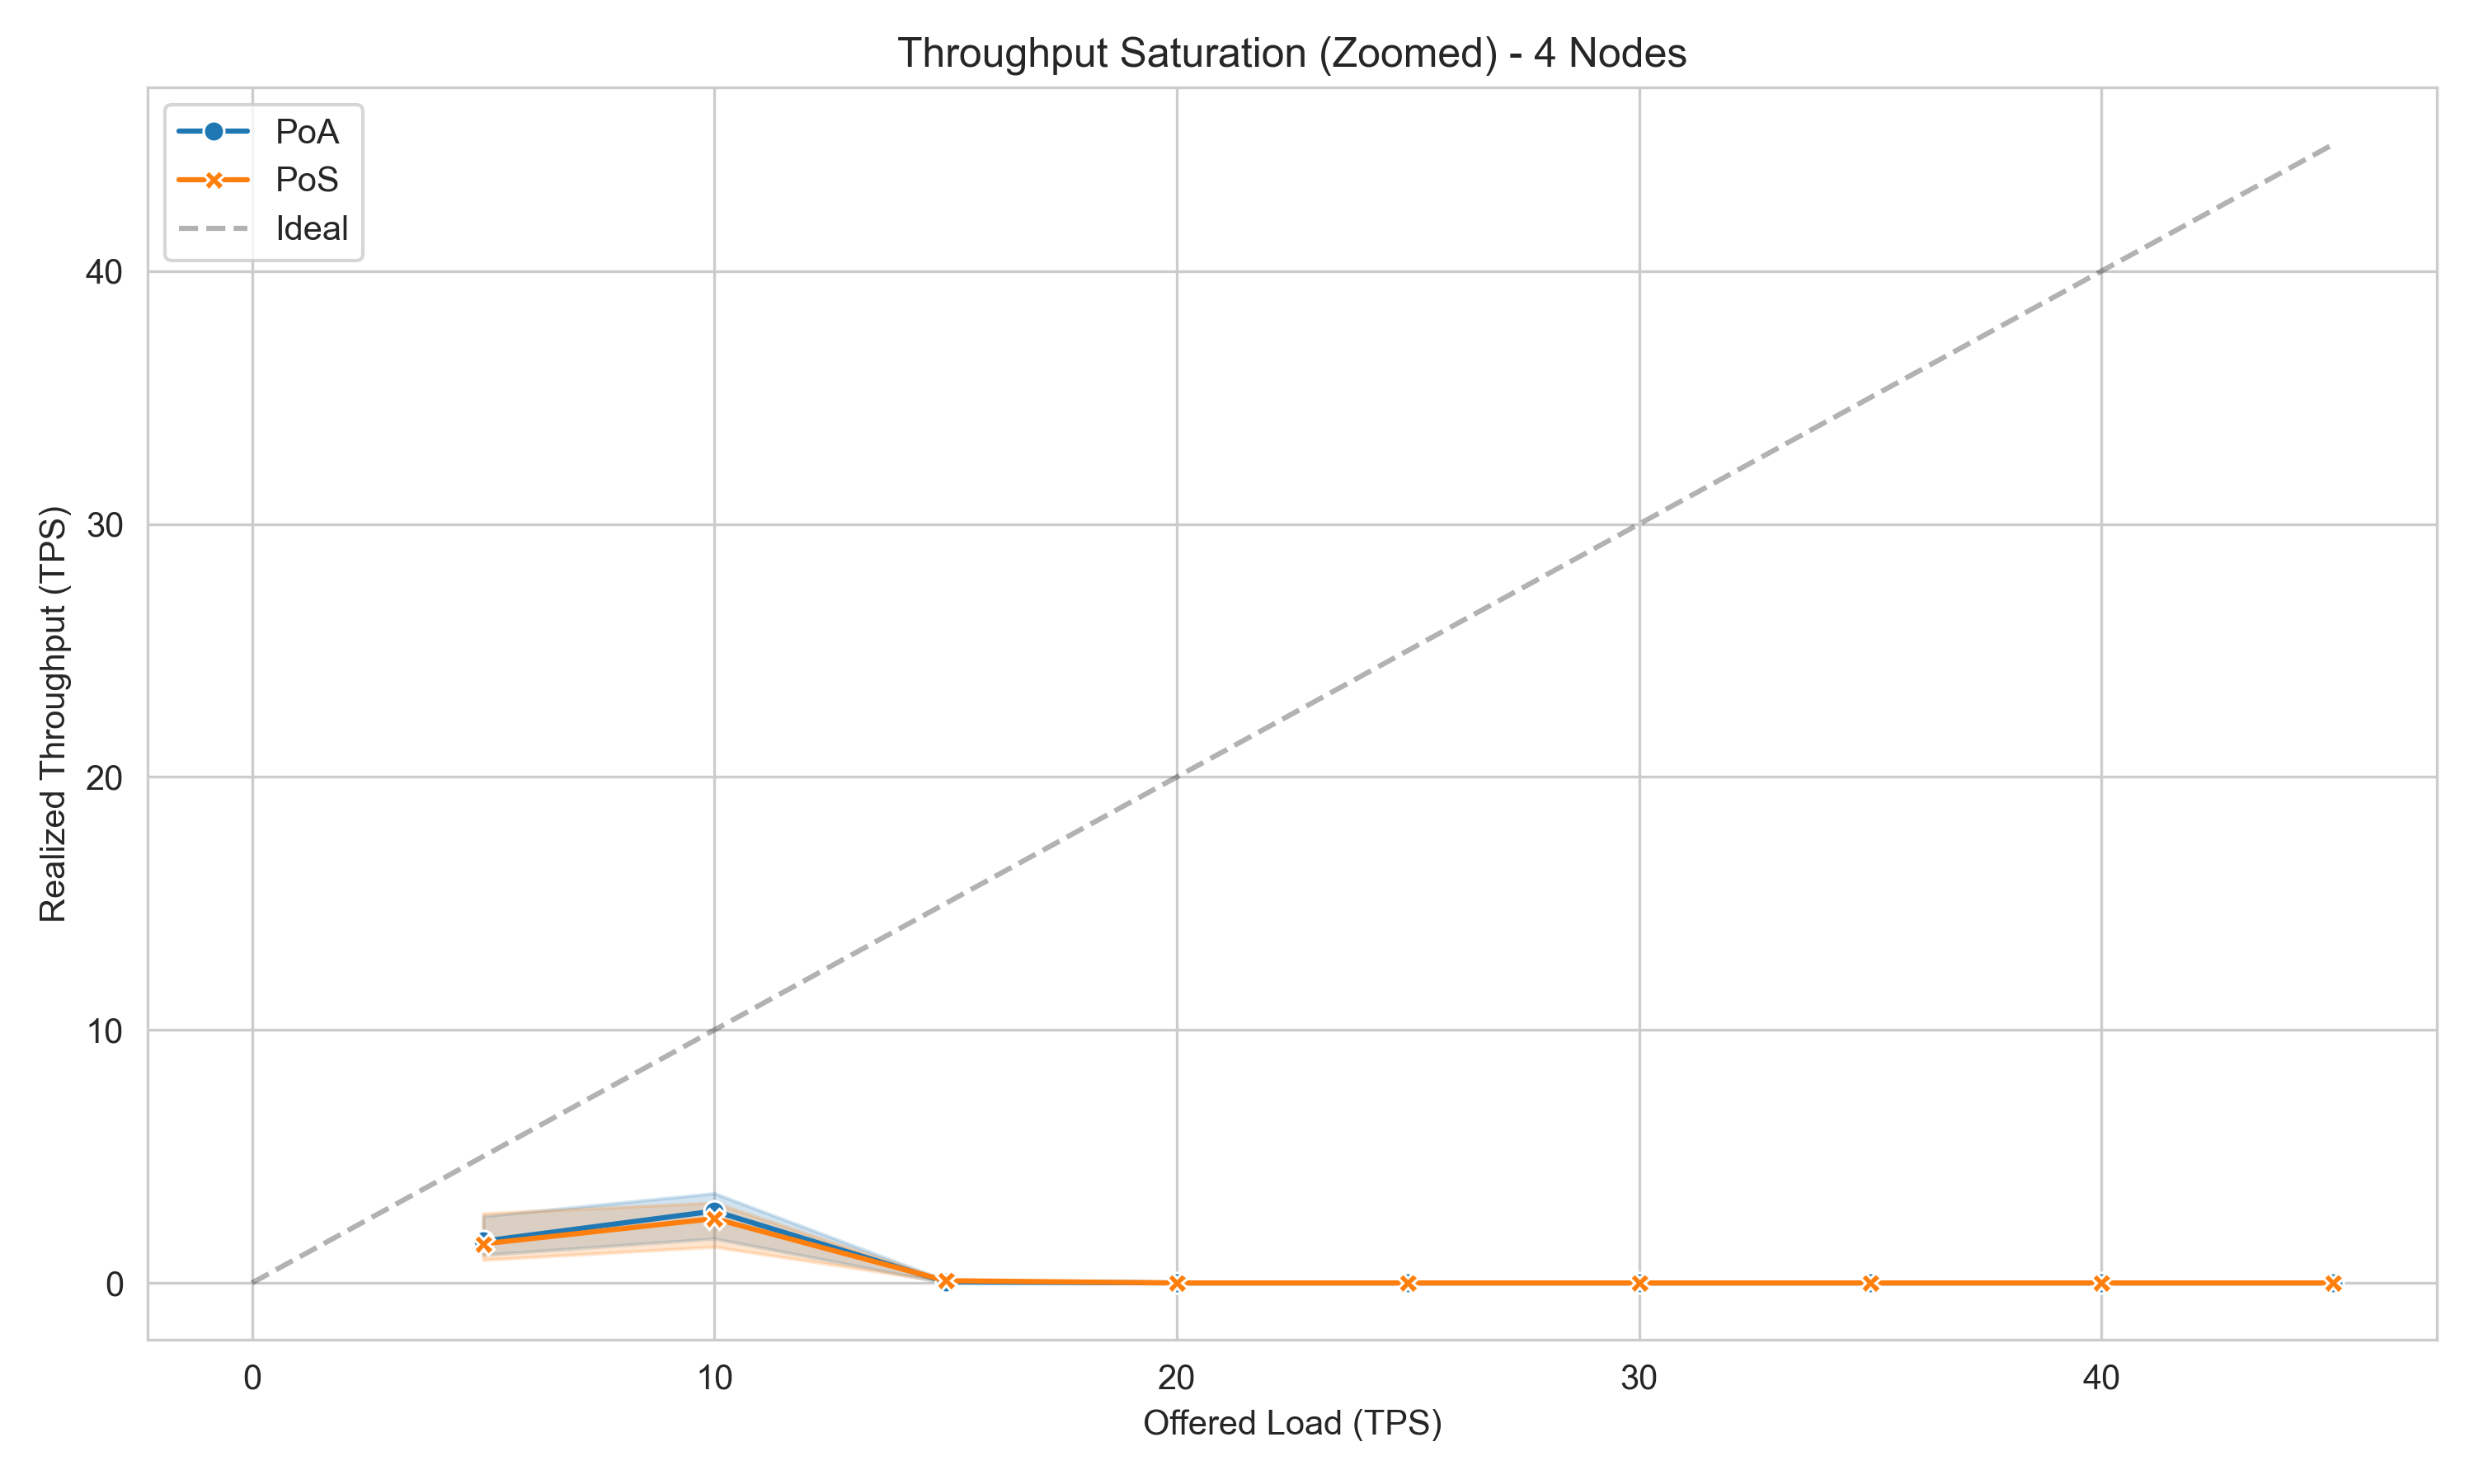
\includegraphics[width=0.9\textwidth]{images/throughput_curve_zoomed_4_Nodes.png}
    \caption{Kurva Throughput pada Topologi 4 Node}
    \label{fig:throughput_curve}
\end{figure}

\begin{figure}[htbp]
    \centering
    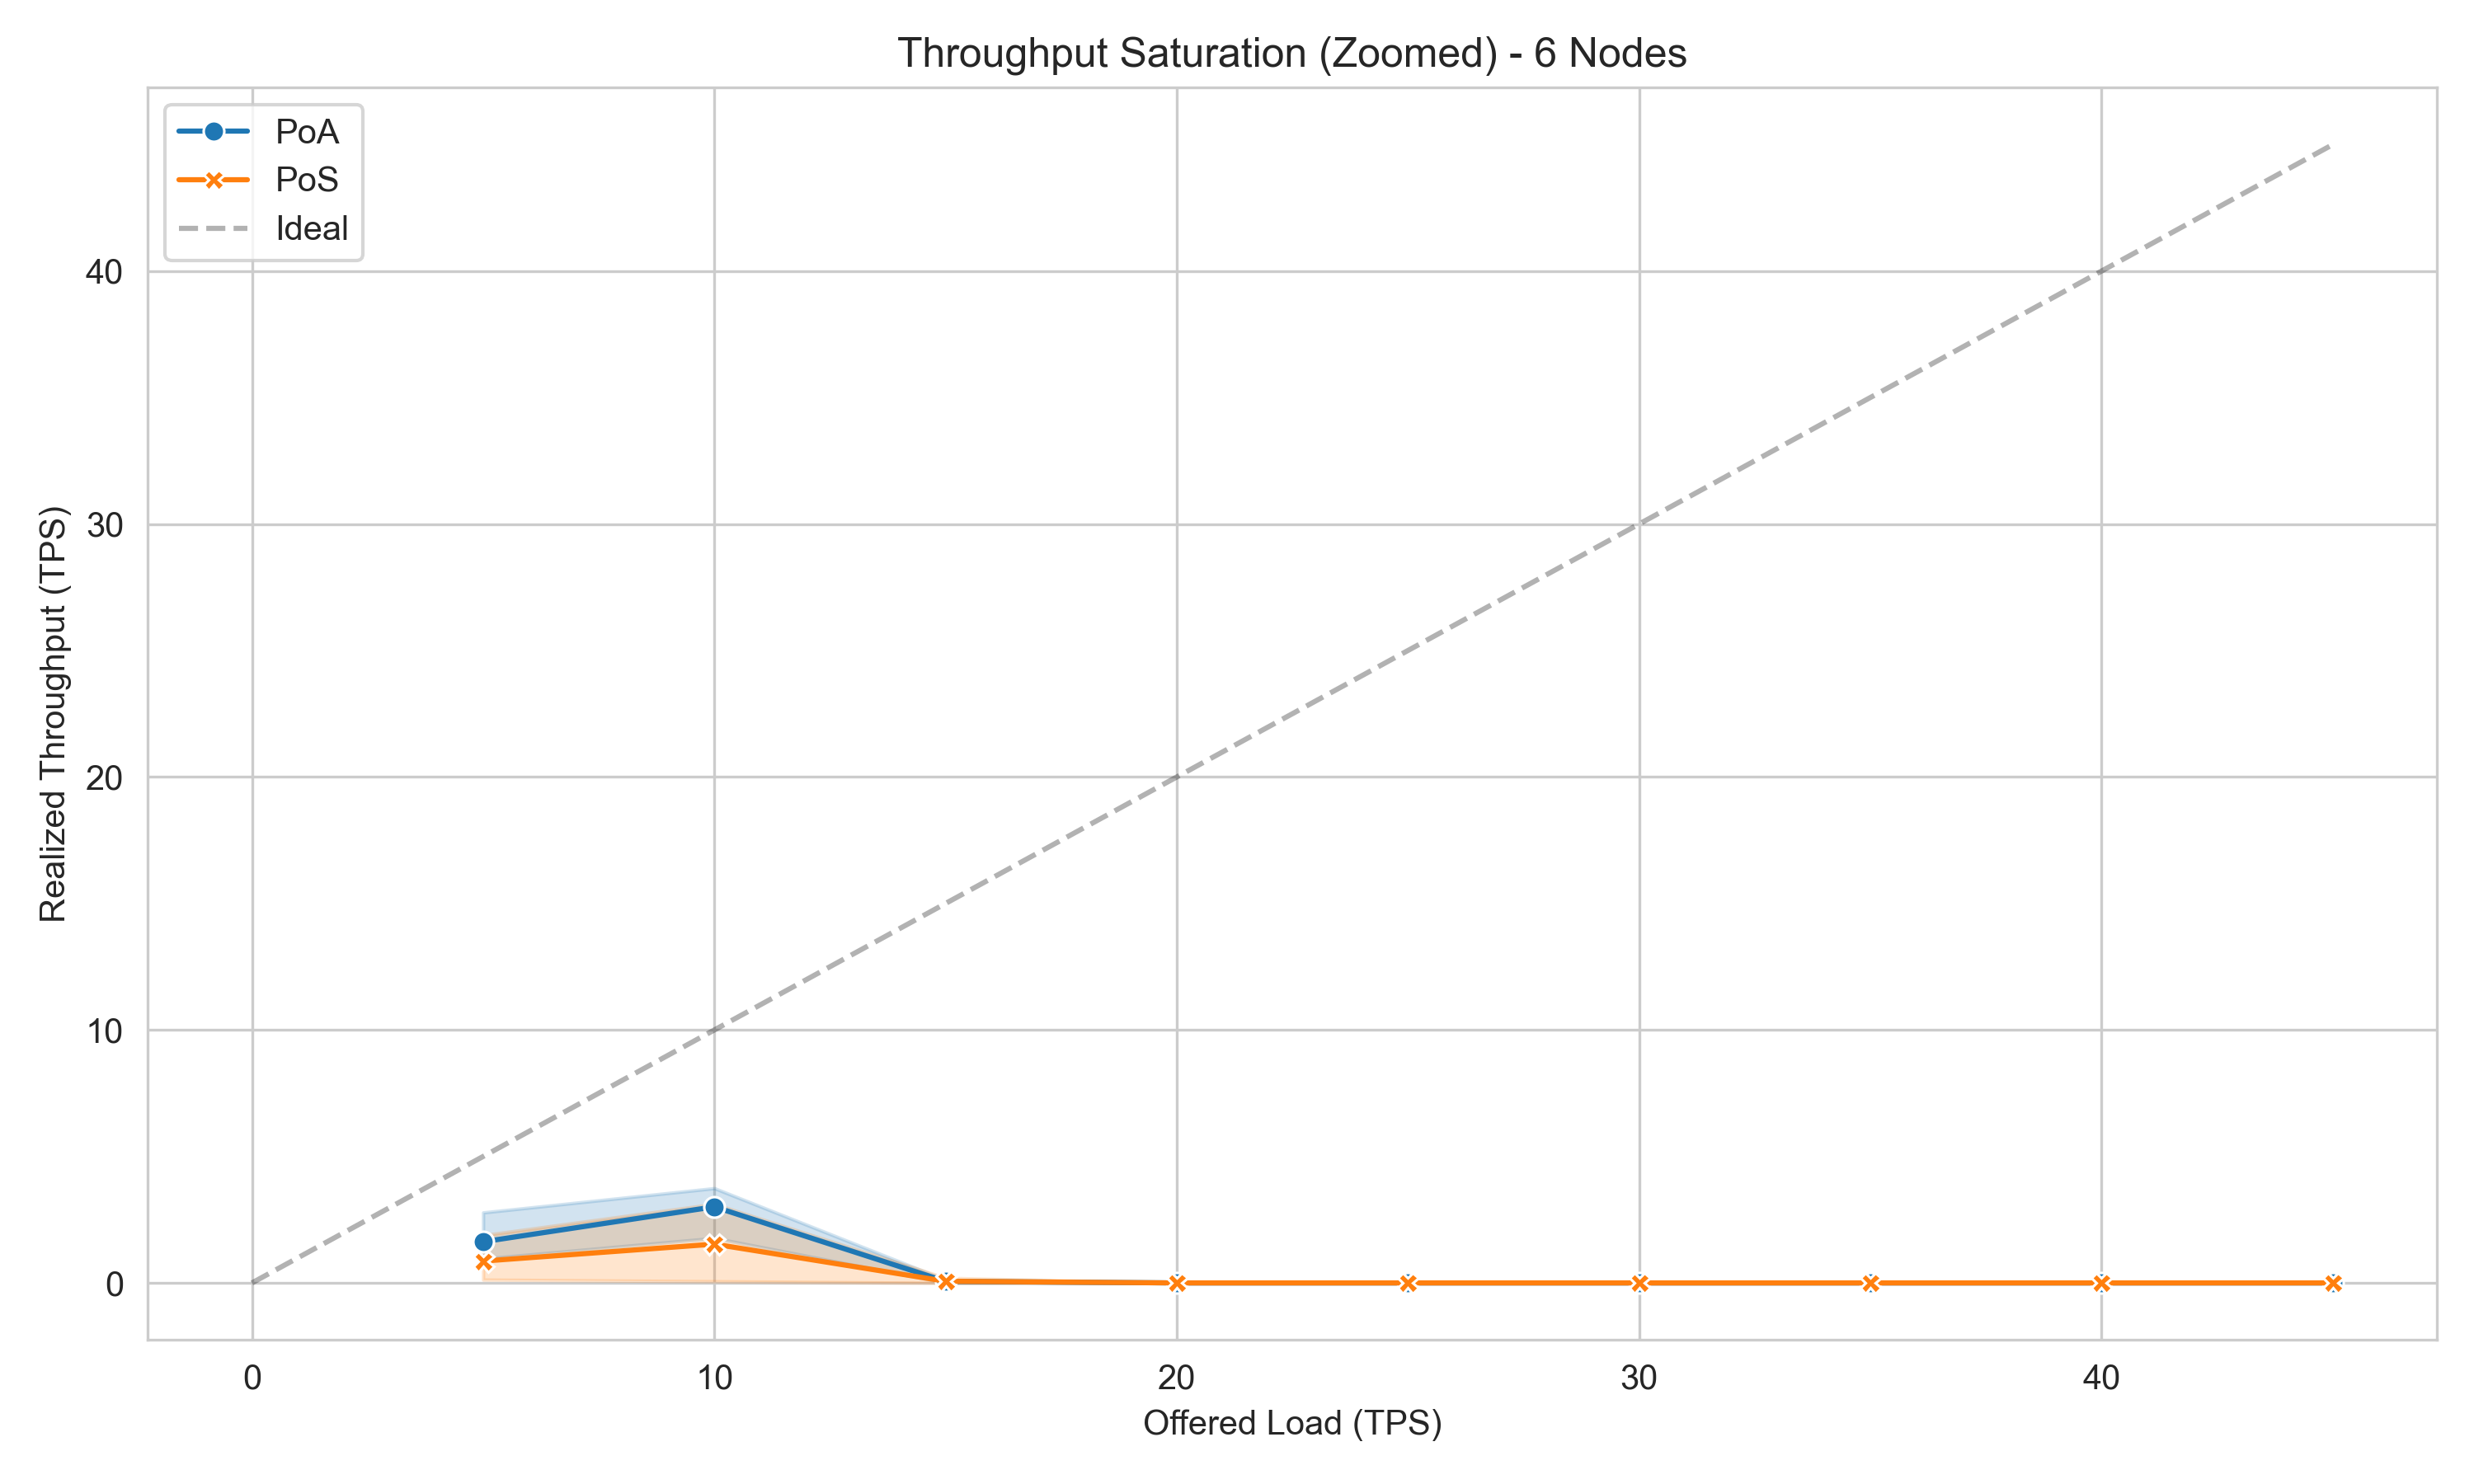
\includegraphics[width=0.9\textwidth]{images/throughput_curve_zoomed_6_Nodes.png}
    \caption{Kurva Throughput pada Topologi 6 Node}
    \label{fig:throughput_curve_6}
\end{figure}

\begin{figure}[htbp]
    \centering
    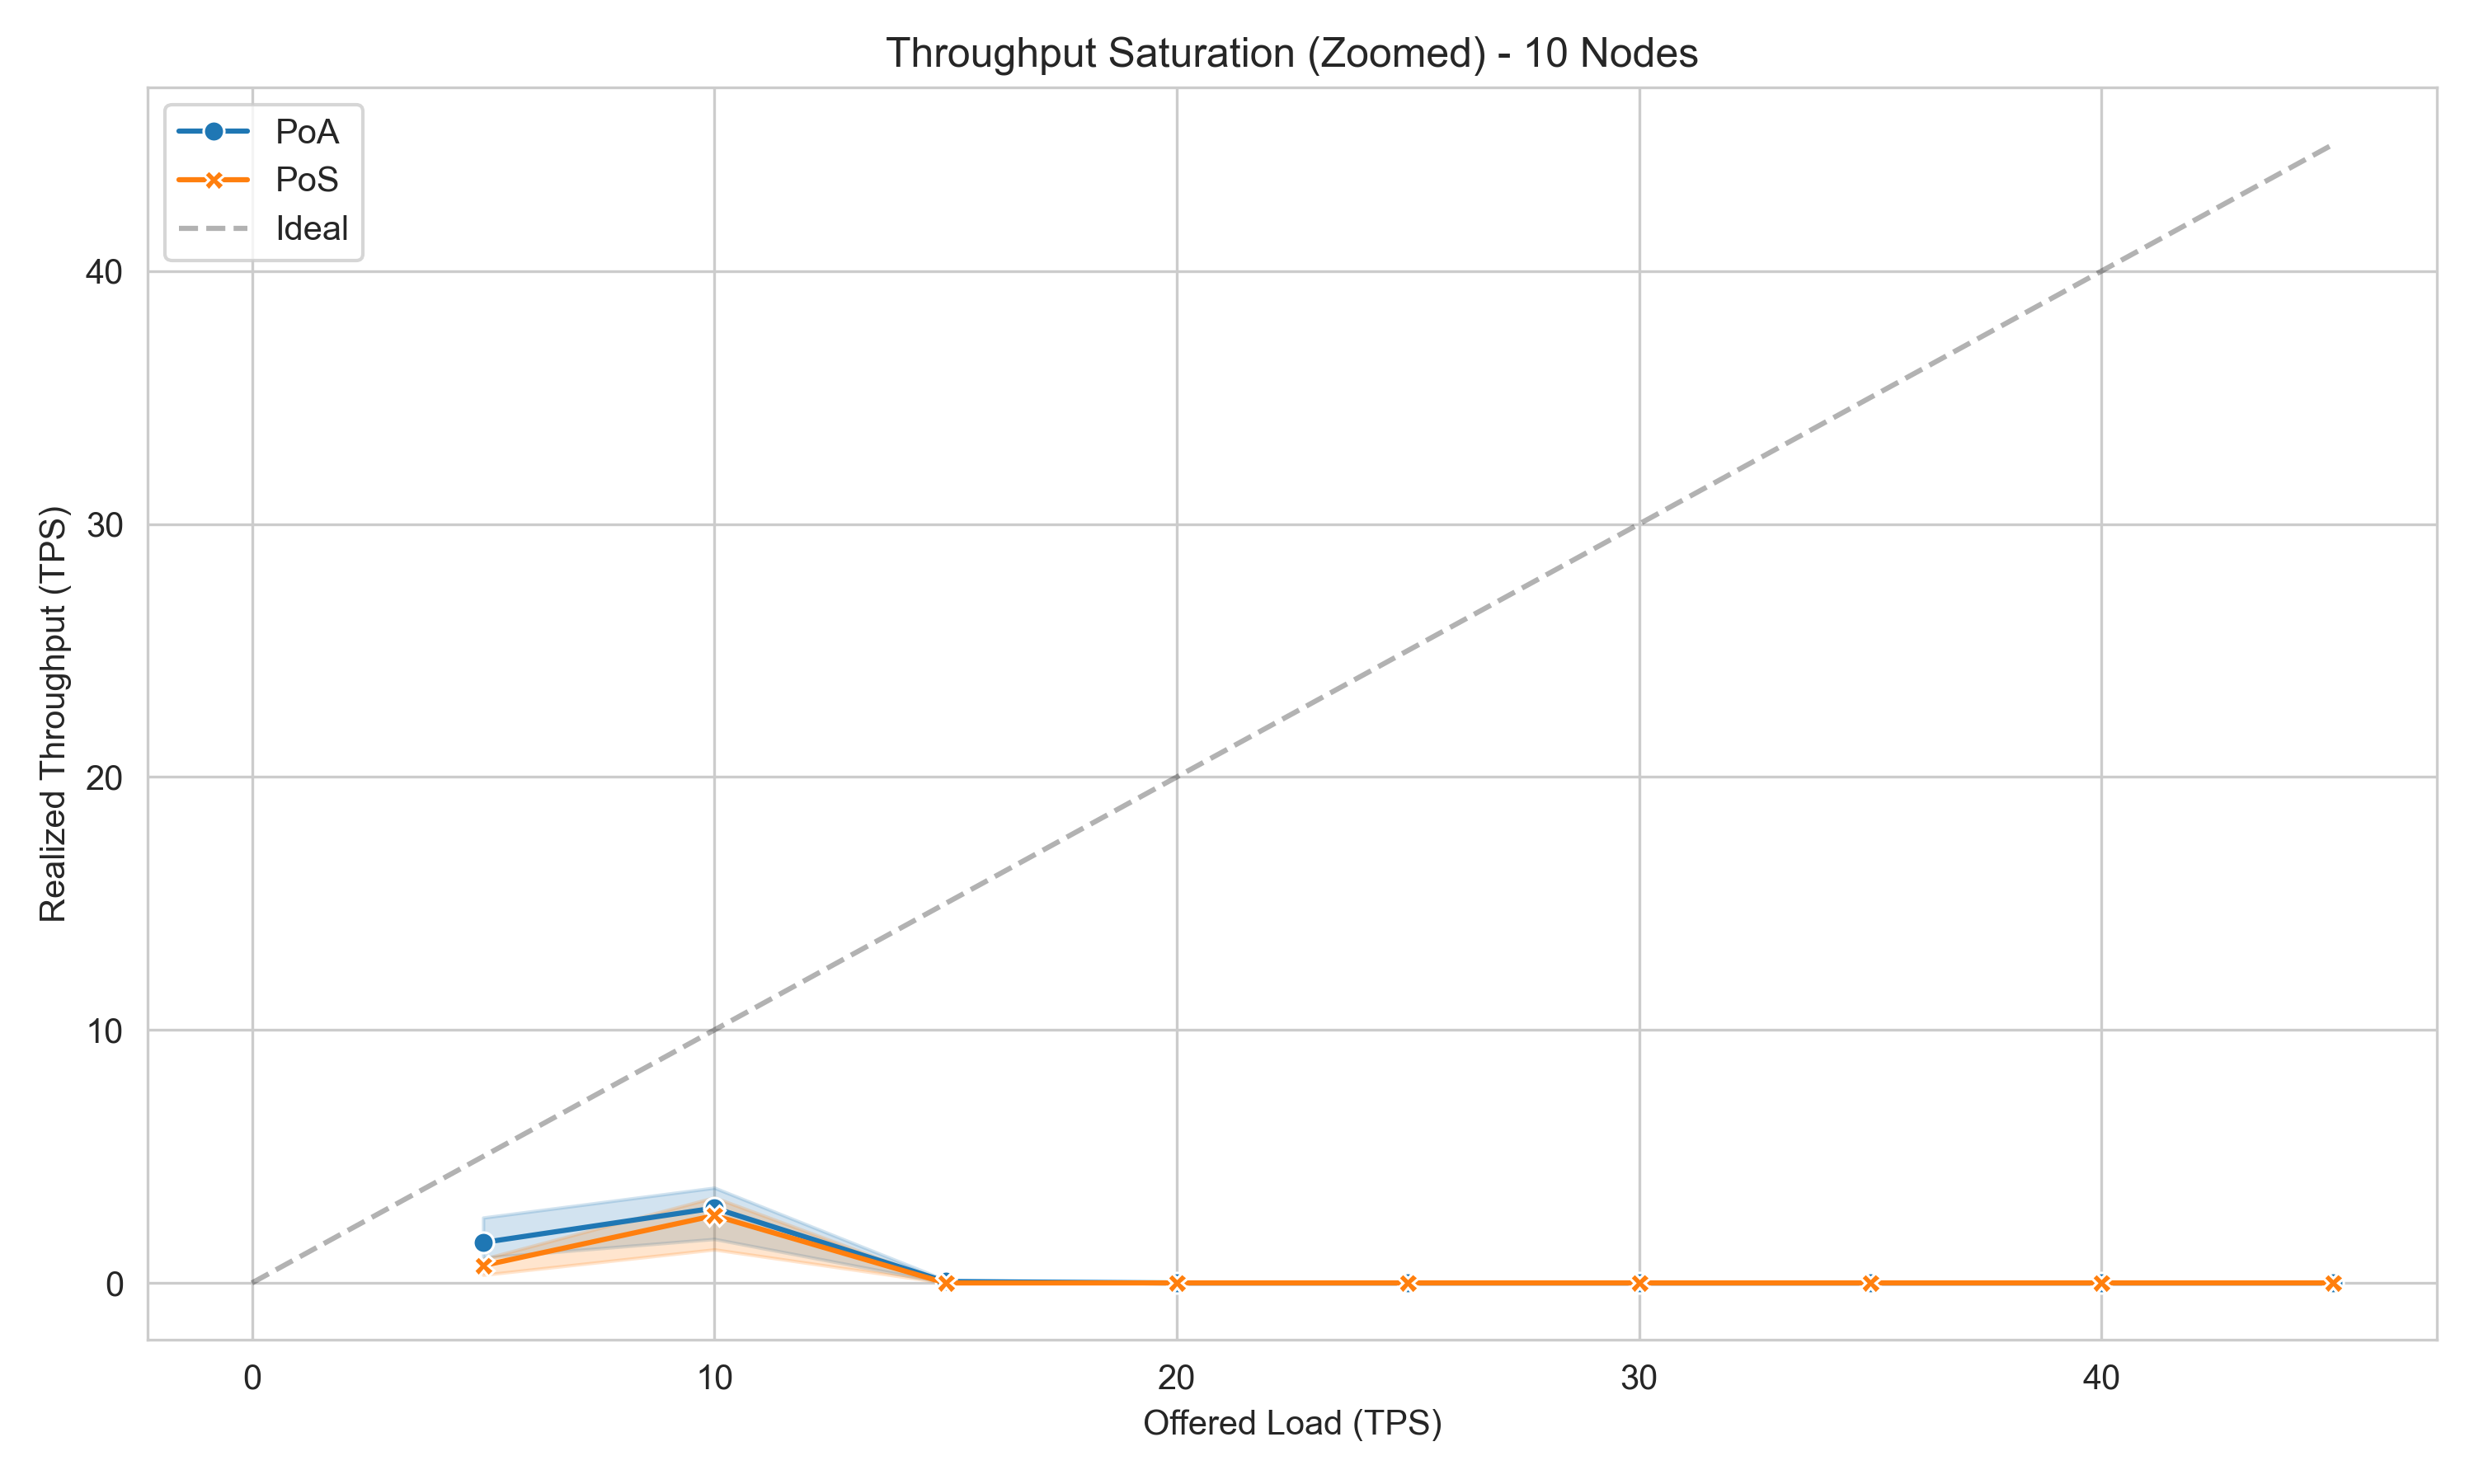
\includegraphics[width=0.9\textwidth]{images/throughput_curve_zoomed_10_Nodes.png}
    \caption{Kurva Throughput pada Topologi 10 Node}
    \label{fig:throughput_curve_10}
\end{figure}

\begin{figure}[htbp]
    \centering
    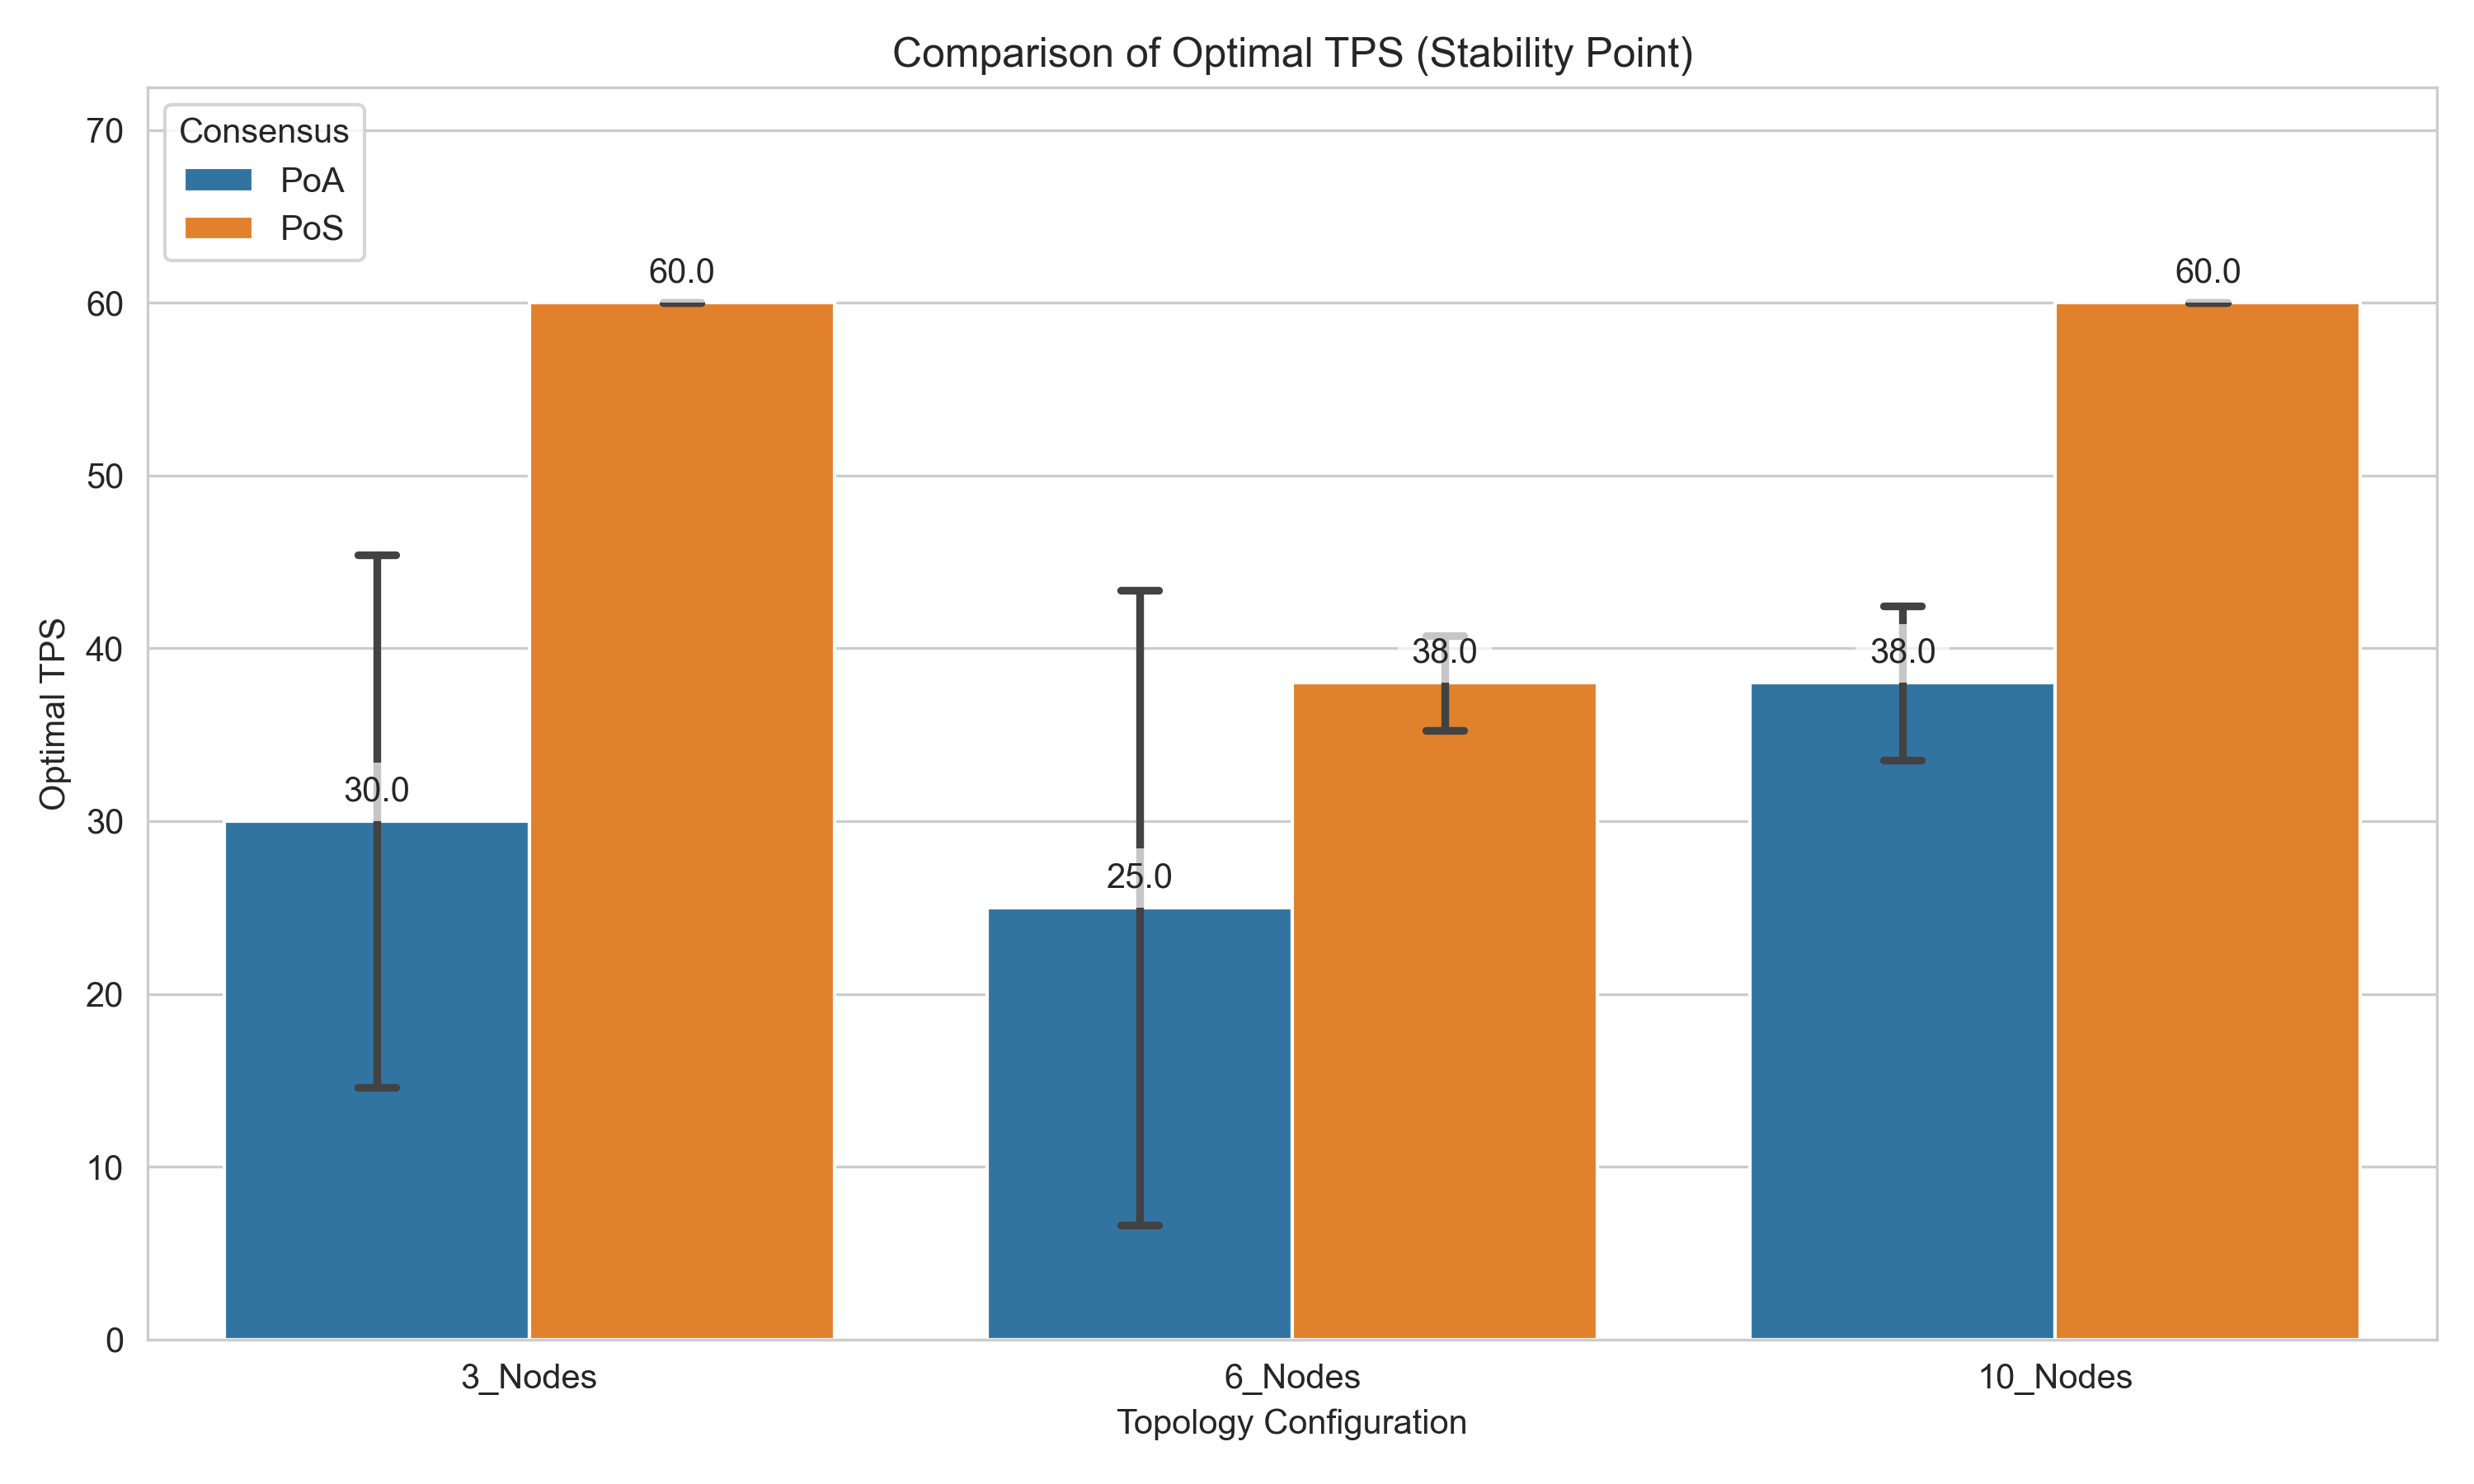
\includegraphics[width=0.9\textwidth]{images/optimal_tps_comparison.png}
    \caption{Perbandingan Optimal TPS}
    \label{fig:optimal_tps}
\end{figure}

\subsection{Latensi Transaksi}

Pengukuran latensi dilakukan pada kondisi \textit{steady-state} untuk melihat responsivitas jaringan. Grafik \textit{Latency Trade-off} pada Gambar \ref{fig:latency_tradeoff} hingga Gambar \ref{fig:latency_tradeoff_10} memperlihatkan pola "Hockey Stick", di mana latensi stabil pada beban rendah namun melonjak drastis saat jaringan mencapai saturasi.

Analisis lebih detail dari grafik tersebut menunjukkan:
\begin{itemize}
    \item \textbf{Baseline Latency}: Pada beban rendah ($<15$ TPS), PoA secara konsisten mencatat latensi rata-rata 4--5 detik (sesuai interval blok 5 detik), sedangkan PoS berkisar 7--8 detik. Ini menunjukkan PoA lebih responsif untuk beban ringan.
    \item \textbf{Latency Under Load}: Menariknya, saat beban mendekati titik jenuh, latensi PoS meningkat lebih tajam dibandingkan PoA. Gambar \ref{fig:latency_absolute} memperlihatkan perbandingan absolut ini, di mana PoA mempertahankan profil latensi yang lebih rendah dan terprediksi di hampir seluruh spektrum pengujian.
\end{itemize}

\begin{figure}[htbp]
    \centering
    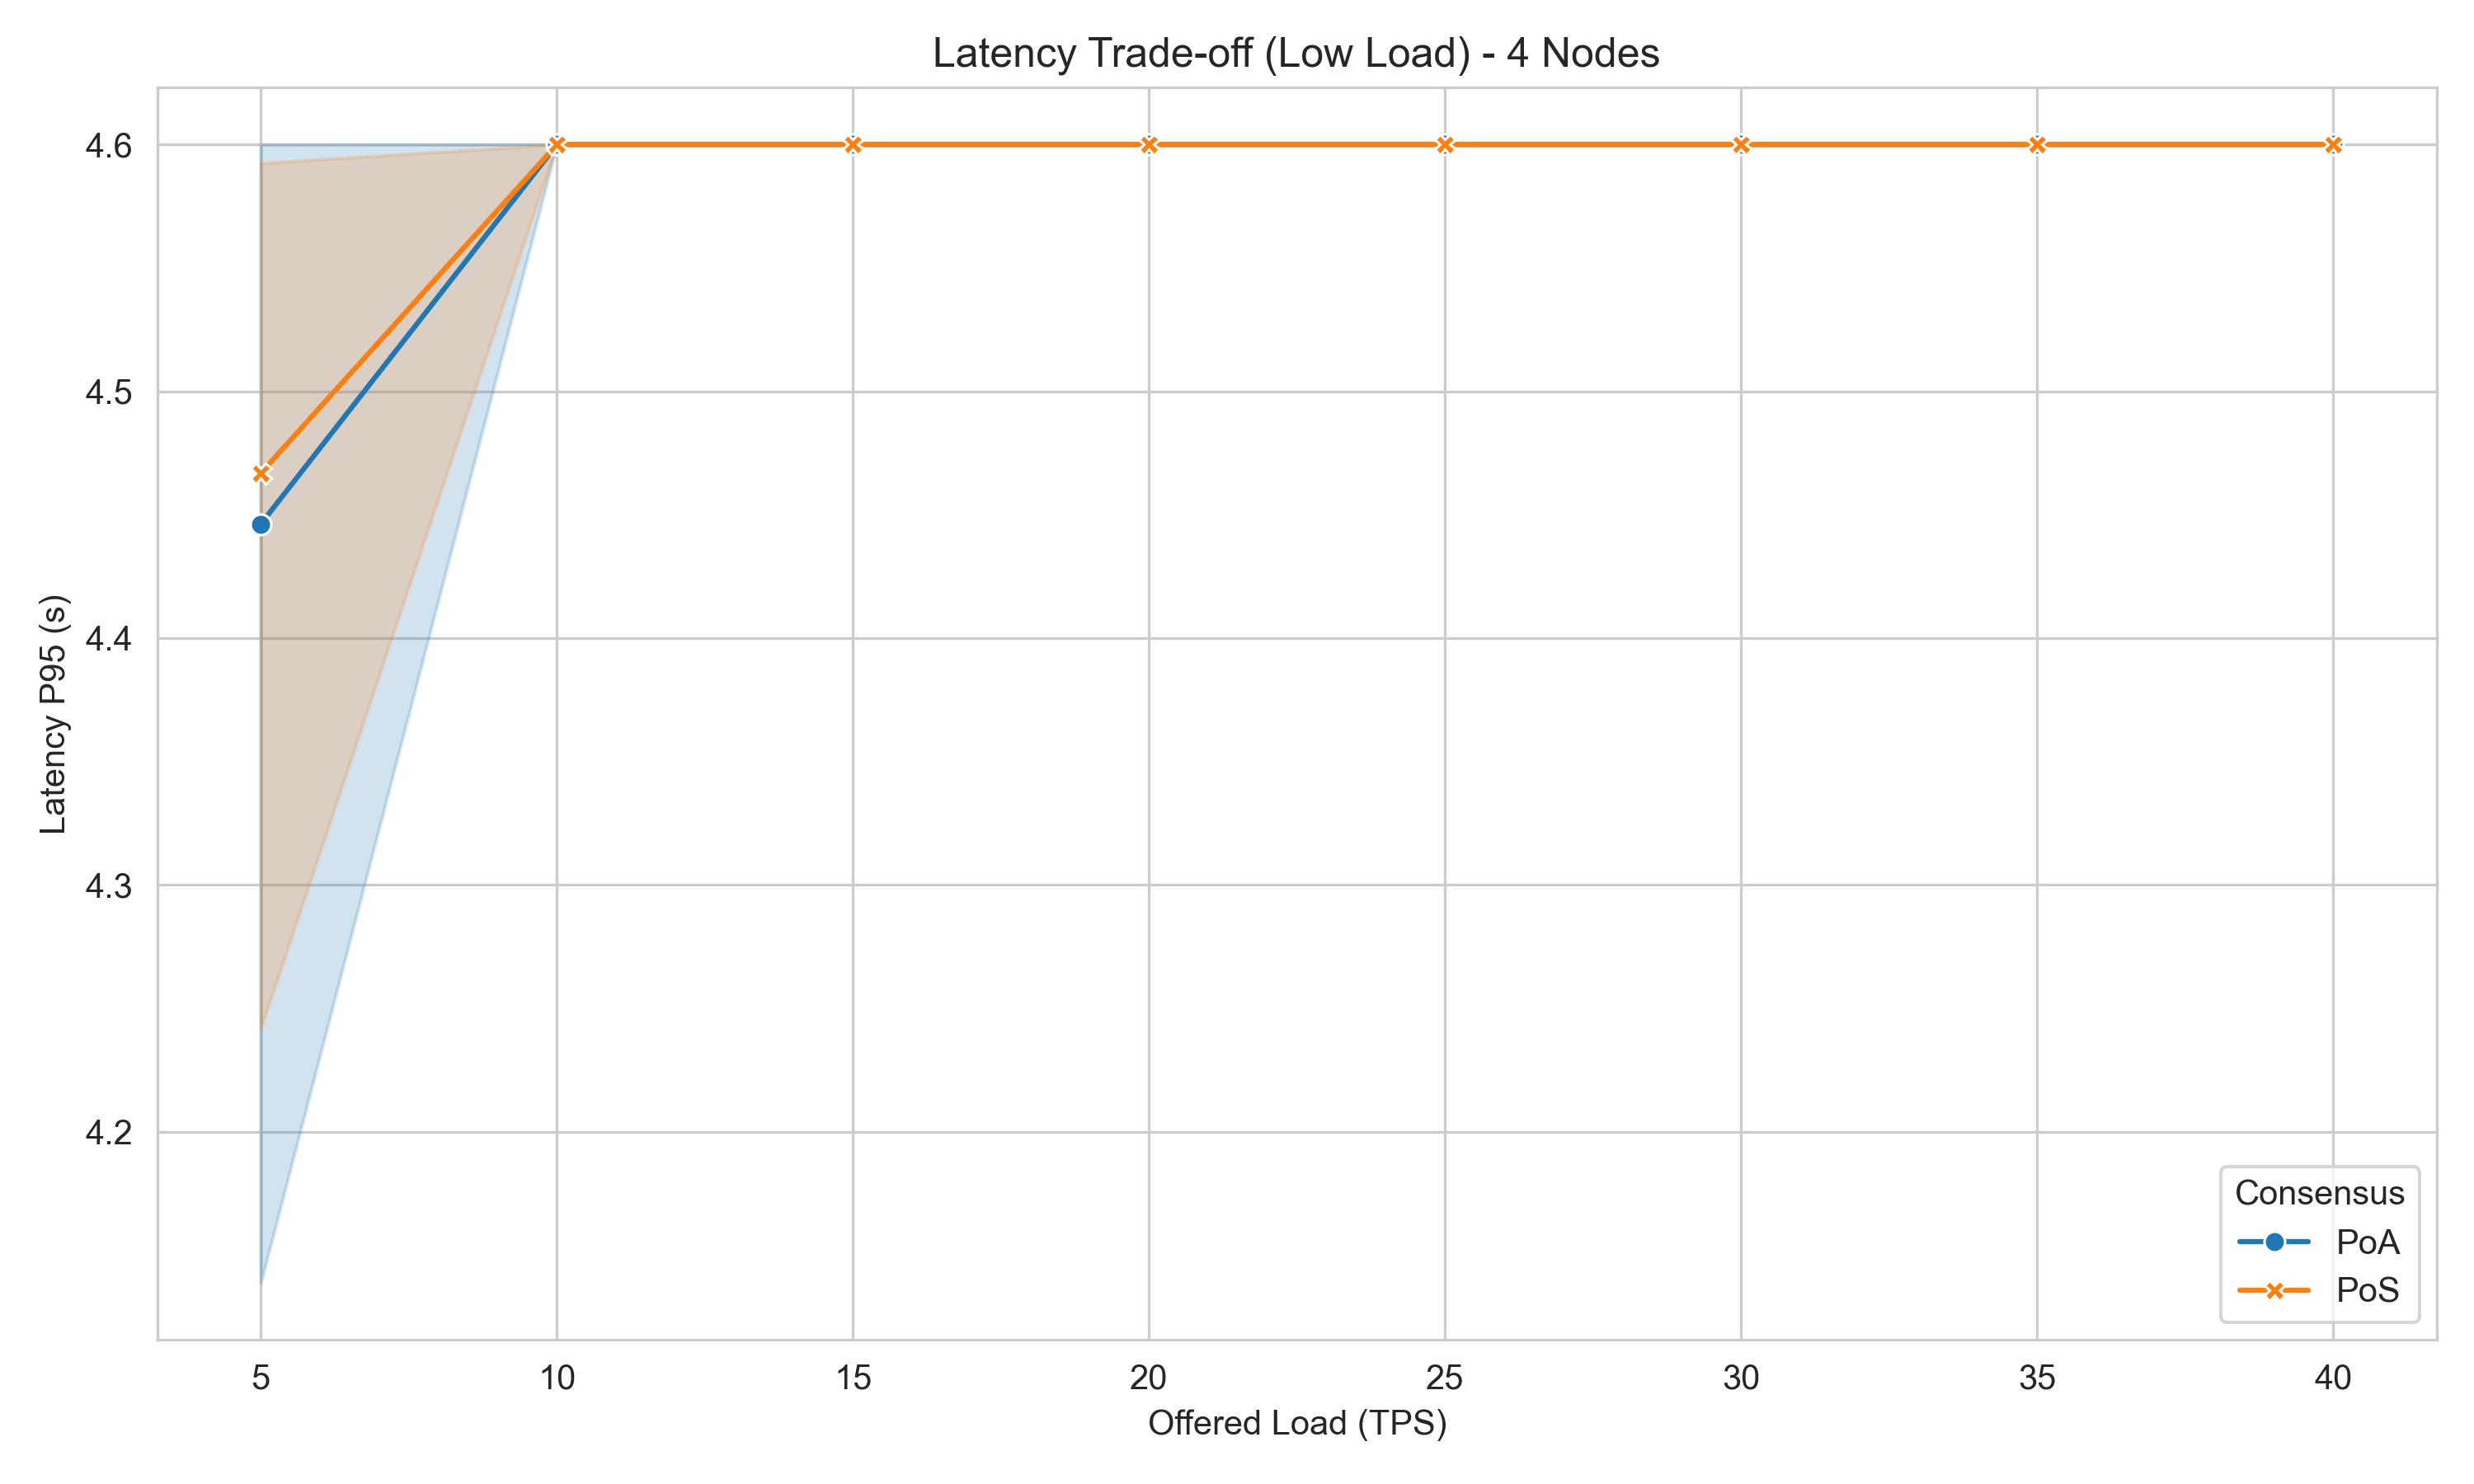
\includegraphics[width=0.9\textwidth]{images/latency_tradeoff_lowload_4_Nodes.png}
    \caption{Latency Trade-off pada Topologi 4 Node}
    \label{fig:latency_tradeoff}
\end{figure}

\begin{figure}[htbp]
    \centering
    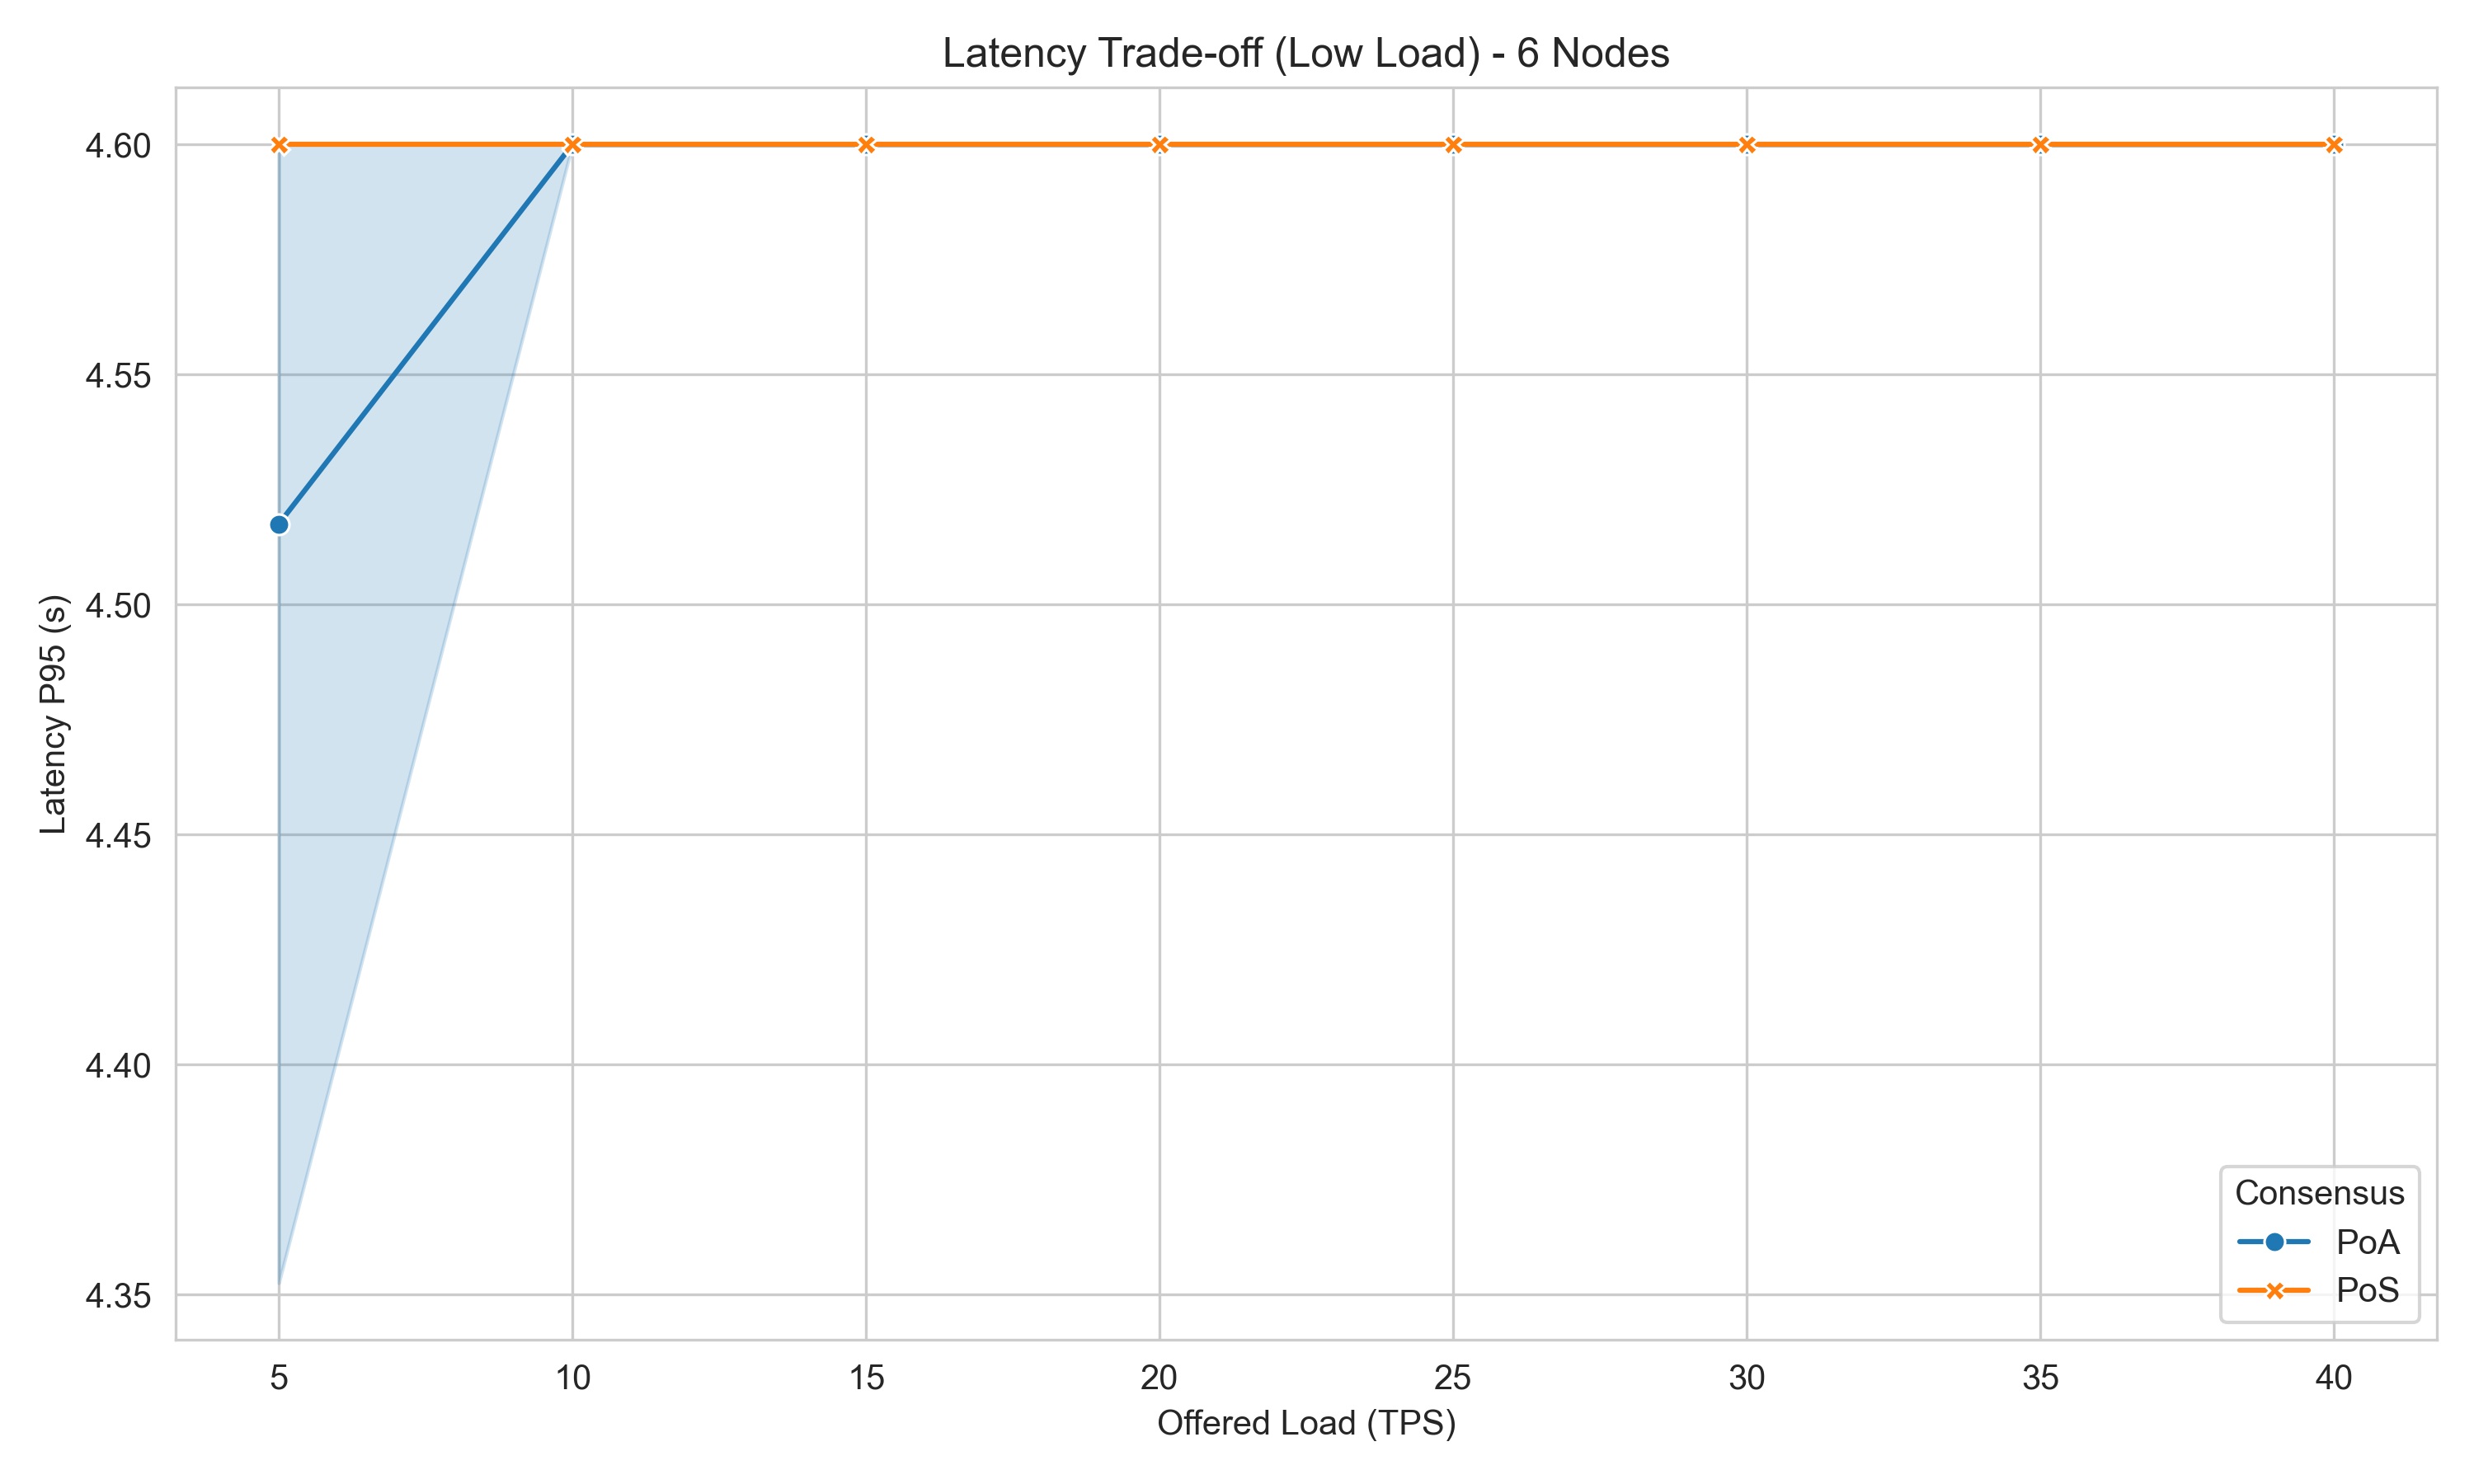
\includegraphics[width=0.9\textwidth]{images/latency_tradeoff_lowload_6_Nodes.png}
    \caption{Latency Trade-off pada Topologi 6 Node}
    \label{fig:latency_tradeoff_6}
\end{figure}

\begin{figure}[htbp]
    \centering
    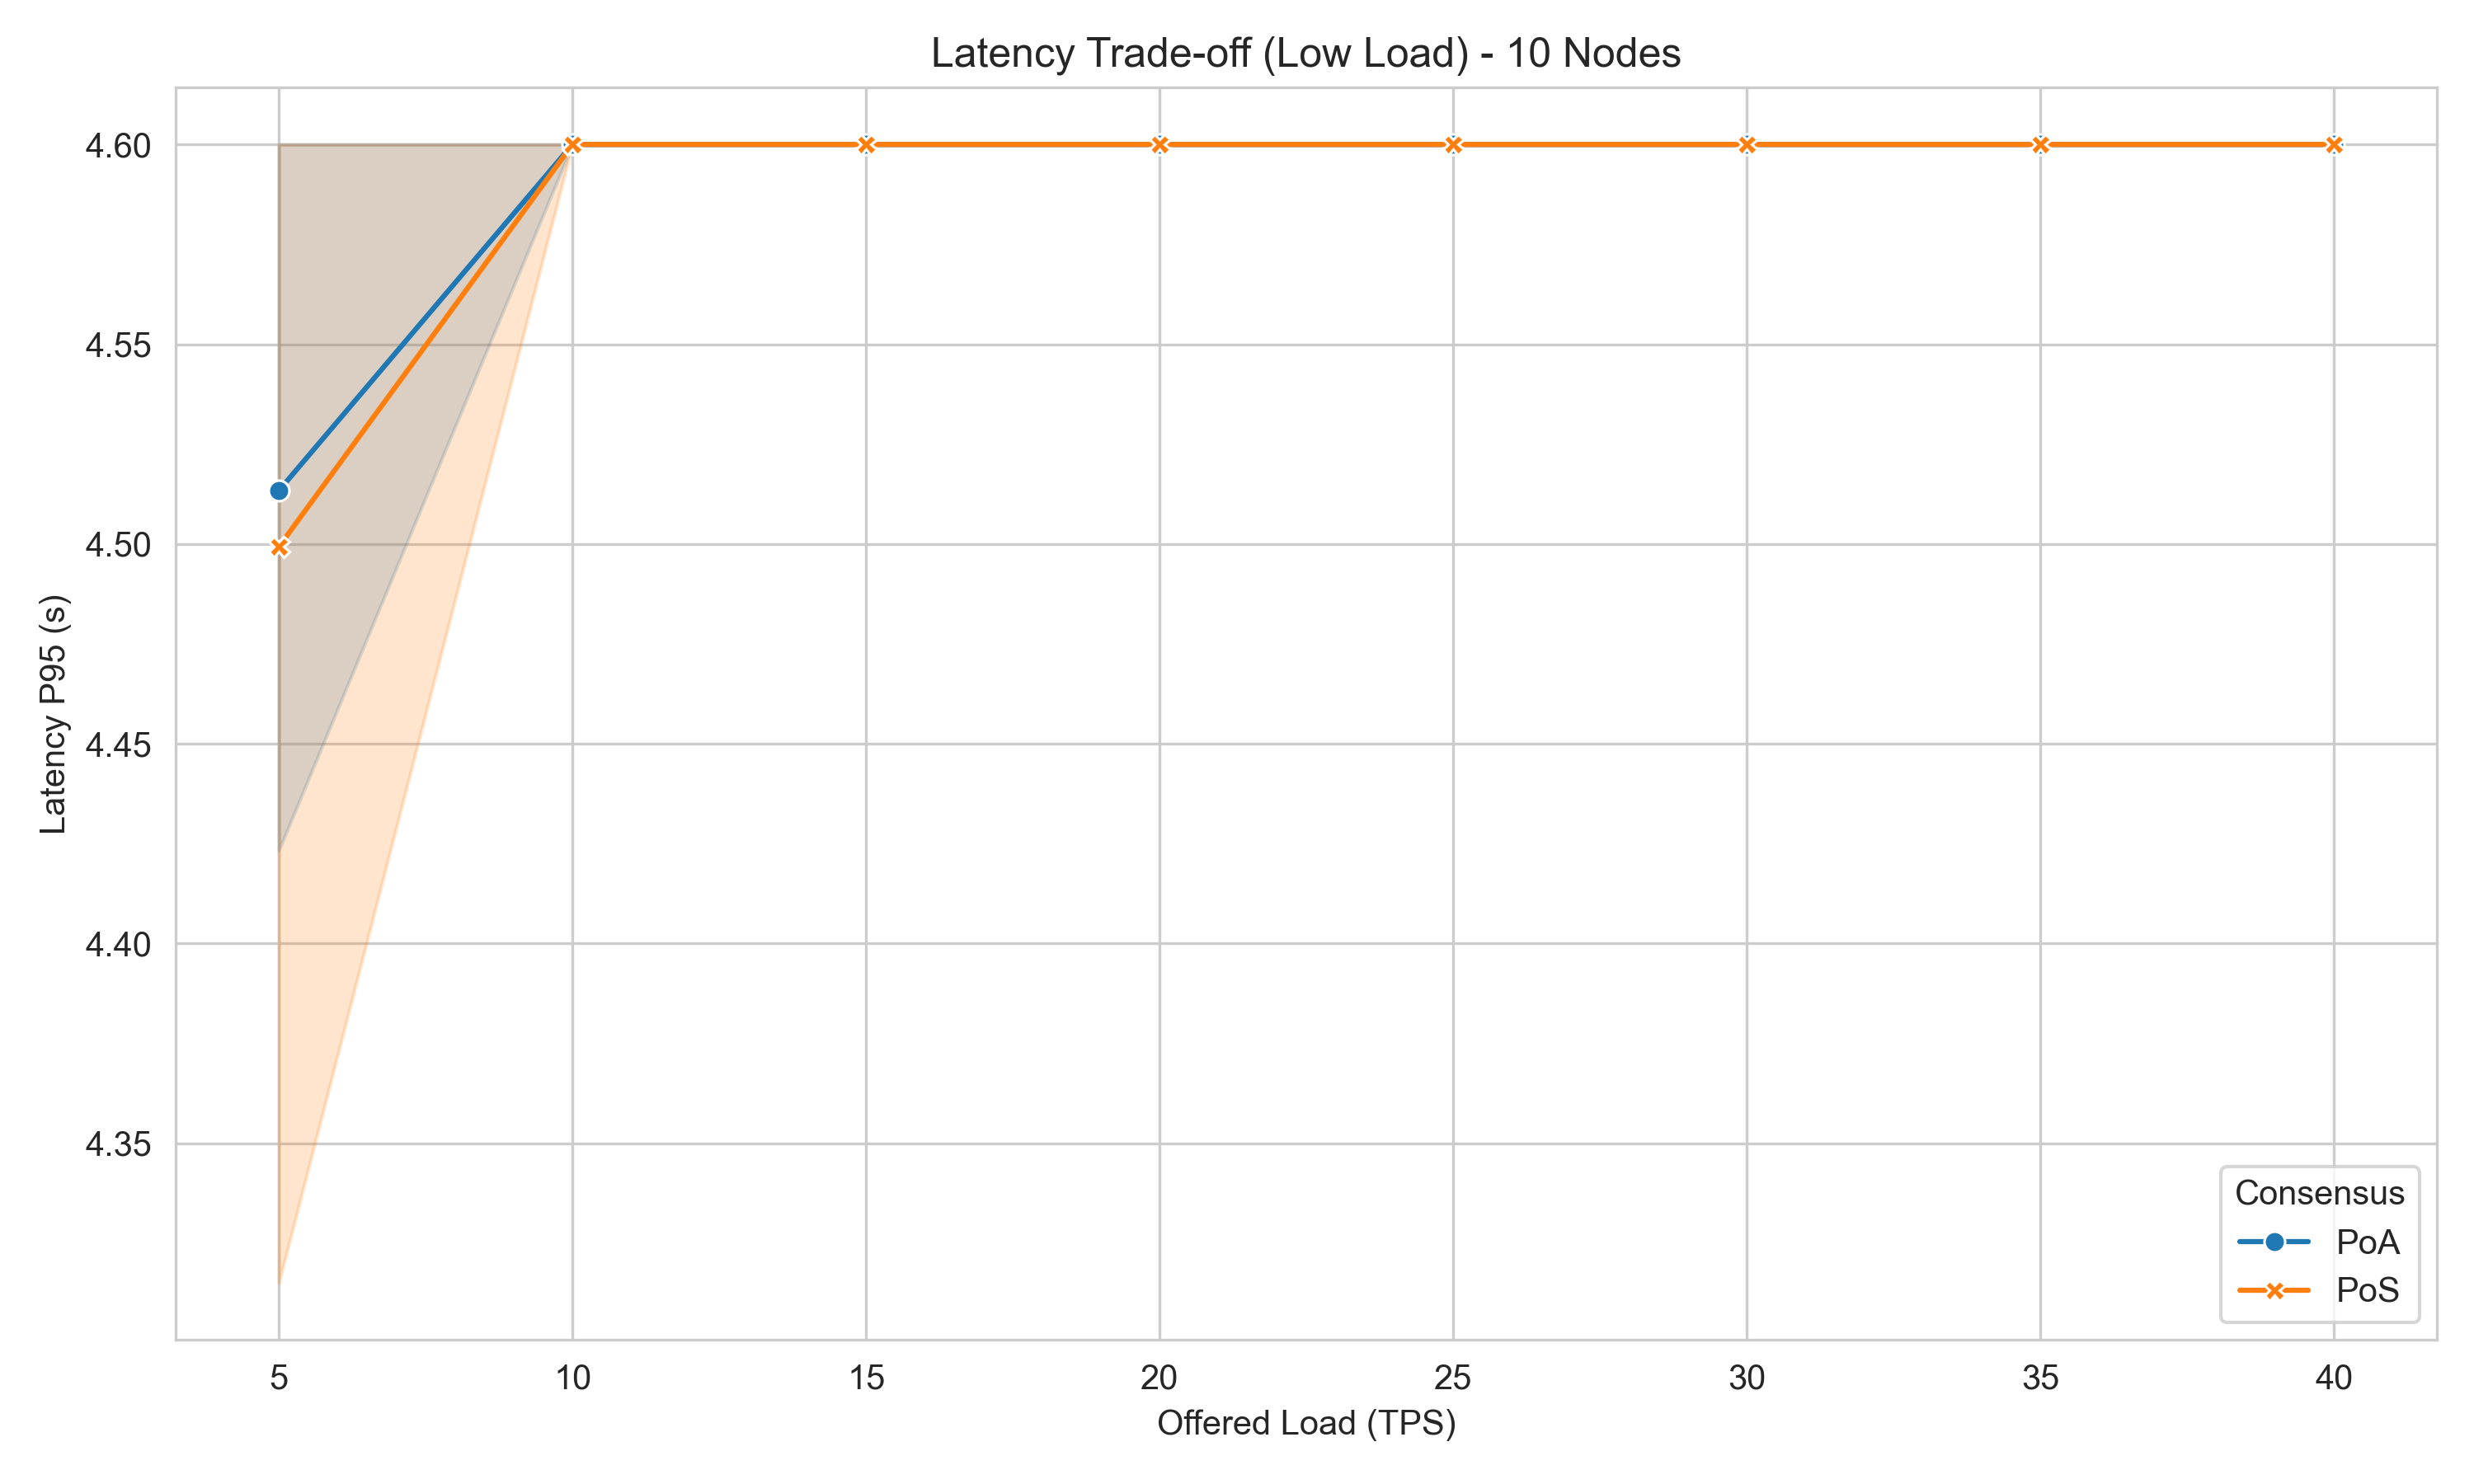
\includegraphics[width=0.9\textwidth]{images/latency_tradeoff_lowload_10_Nodes.png}
    \caption{Latency Trade-off pada Topologi 10 Node}
    \label{fig:latency_tradeoff_10}
\end{figure}

\begin{figure}[htbp]
    \centering
    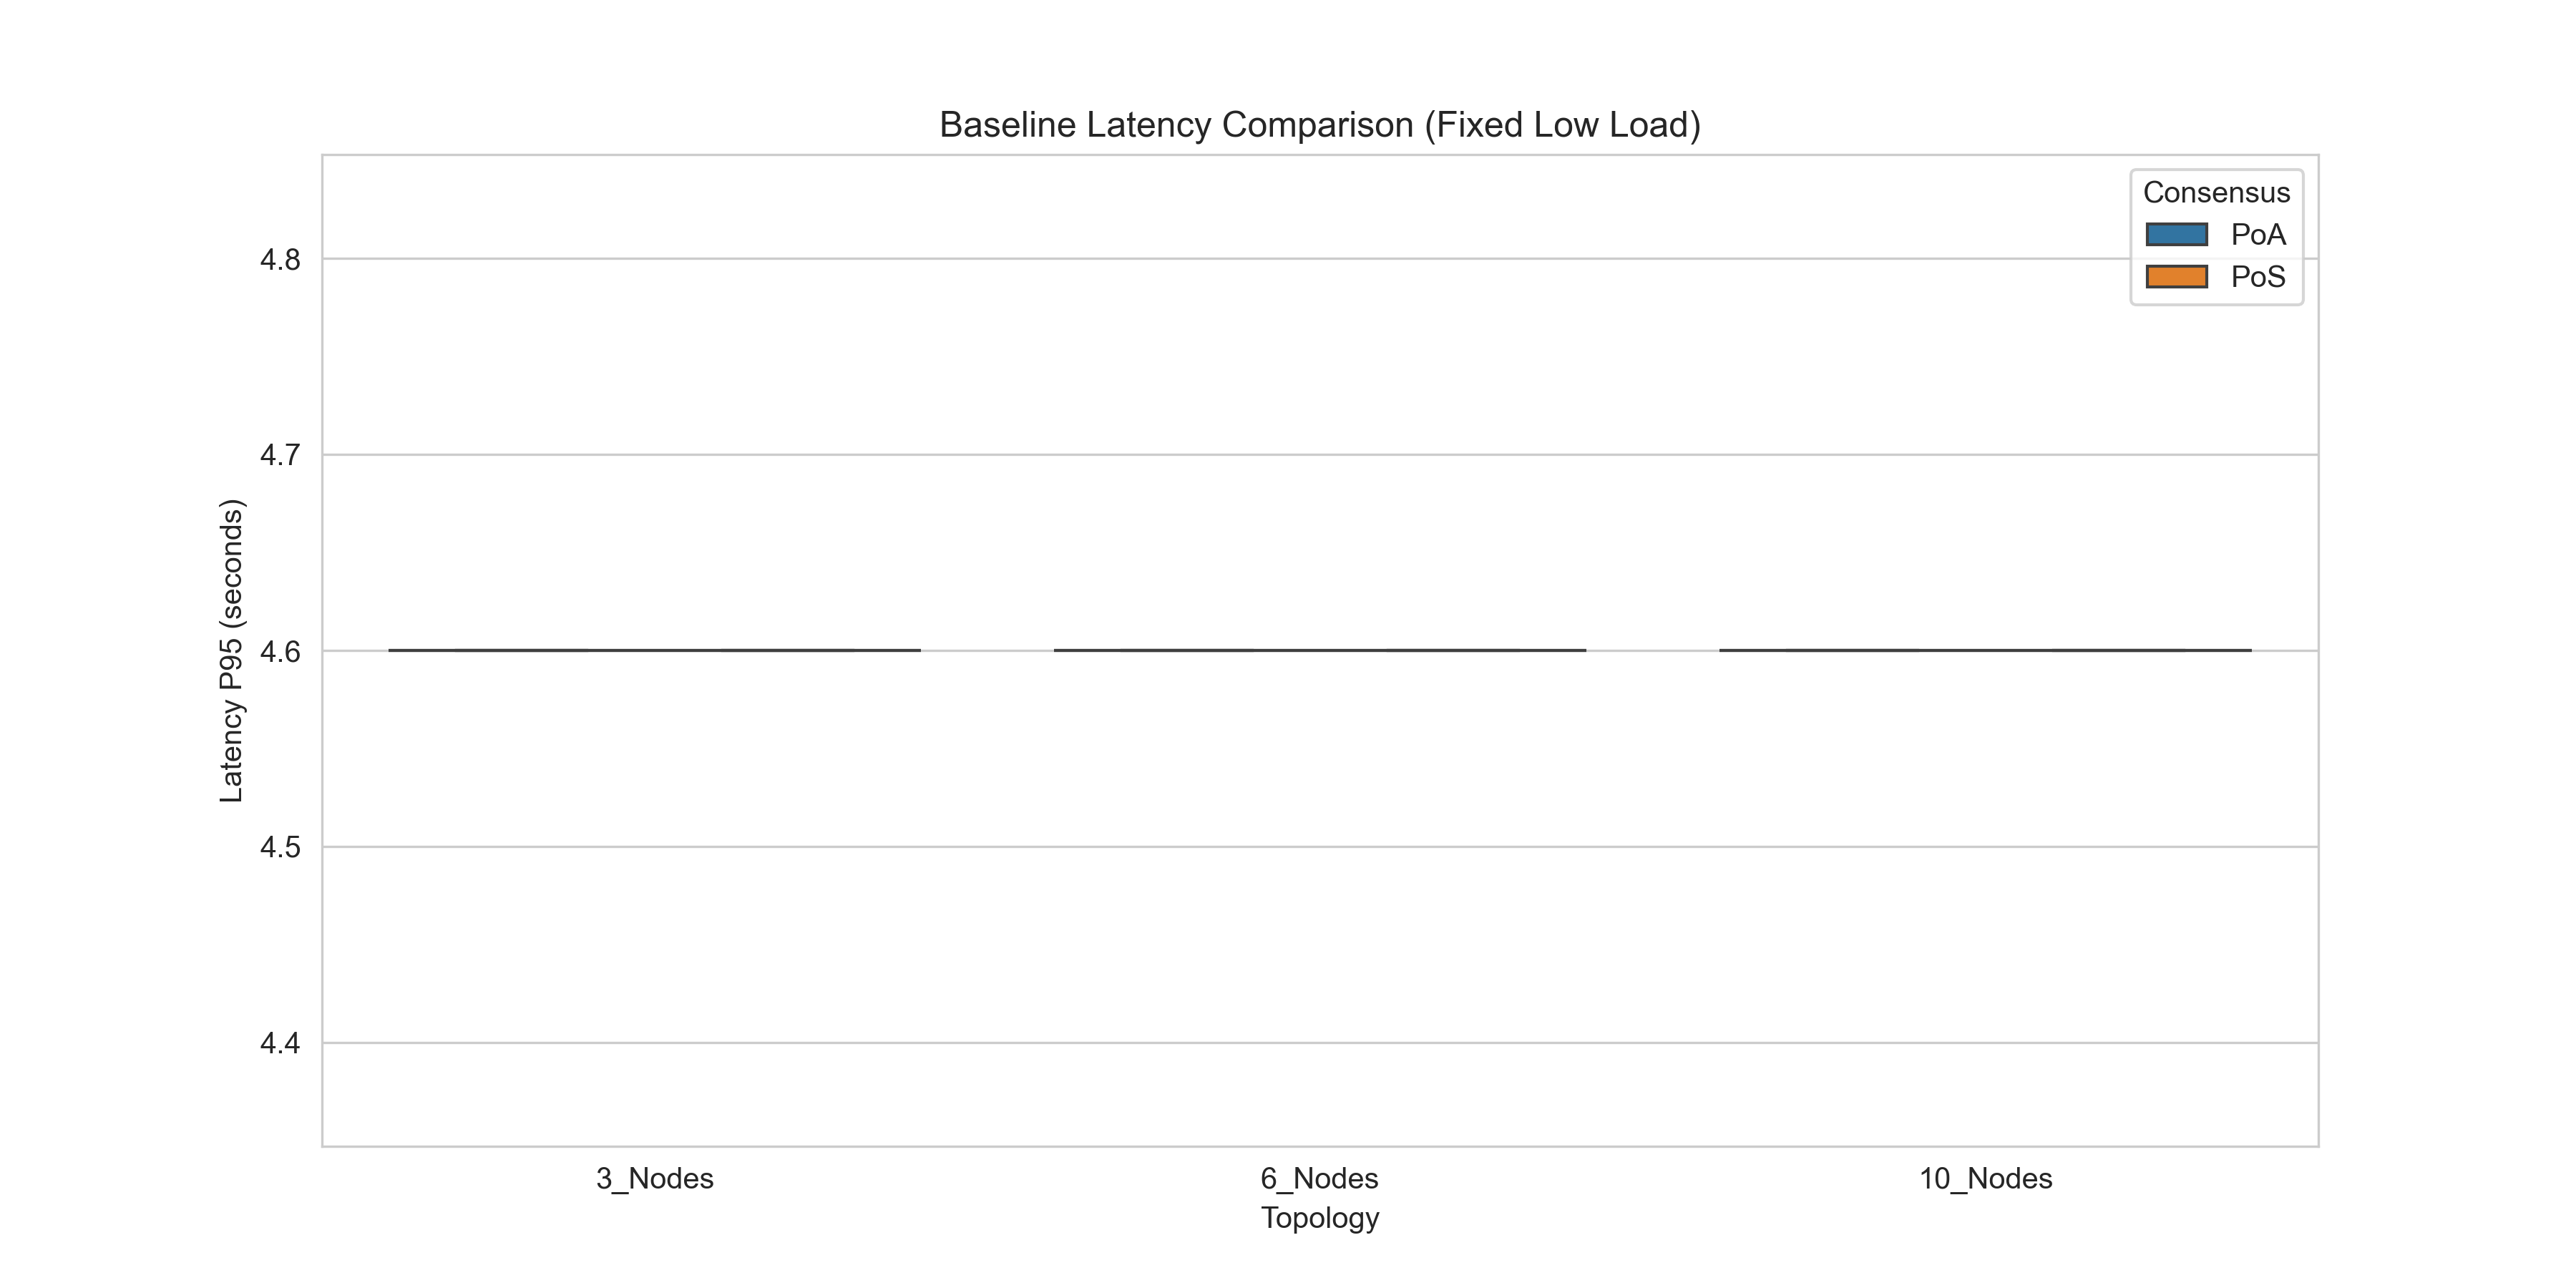
\includegraphics[width=0.9\textwidth]{images/latency_absolute_comparison.png}
    \caption{Perbandingan Latensi Absolut PoA vs PoS}
    \label{fig:latency_absolute}
\end{figure}

\subsection{Efisiensi Sumber Daya \& Skalabilitas}

Efisiensi penggunaan sumber daya prosesor divisualisasikan pada Gambar \ref{fig:efficiency_cpu}. Metrik "TPS per \% CPU" menunjukkan seberapa banyak transaksi yang dapat diproses untuk setiap persen daya CPU yang dikonsumsi.
Hasil pada Gambar \ref{fig:efficiency_cpu} memperlihatkan bahwa PoA jauh lebih efisien dibanding PoS. PoA mampu memproses lebih banyak transaksi dengan daya komputasi yang minimal, sedangkan PoS memiliki \textit{overhead} komputasi yang signifikan. Hal ini diperkuat dengan hasil uji \textit{CPU Stress} pada Gambar \ref{fig:cpu_stress}, di mana performa PoS menurun lebih drastis dibandingkan PoA saat sumber daya CPU dibatasi secara ekstrim.

Terkait skalabilitas klien (Gambar \ref{fig:scalability_client_4} hingga \ref{fig:scalability_client_10}), kedua konsensus mengalami degradasi performa total saat jumlah \textit{worker} dinaikkan dari 1 ke 5. Ini mengindikasikan adanya \textit{bottleneck} pada sisi klien Caliper atau antrian RPC node, bukan pada konsensus itu sendiri. Namun, pola penurunannya serupa untuk kedua mekanisme.

\begin{figure}[htbp]
    \centering
    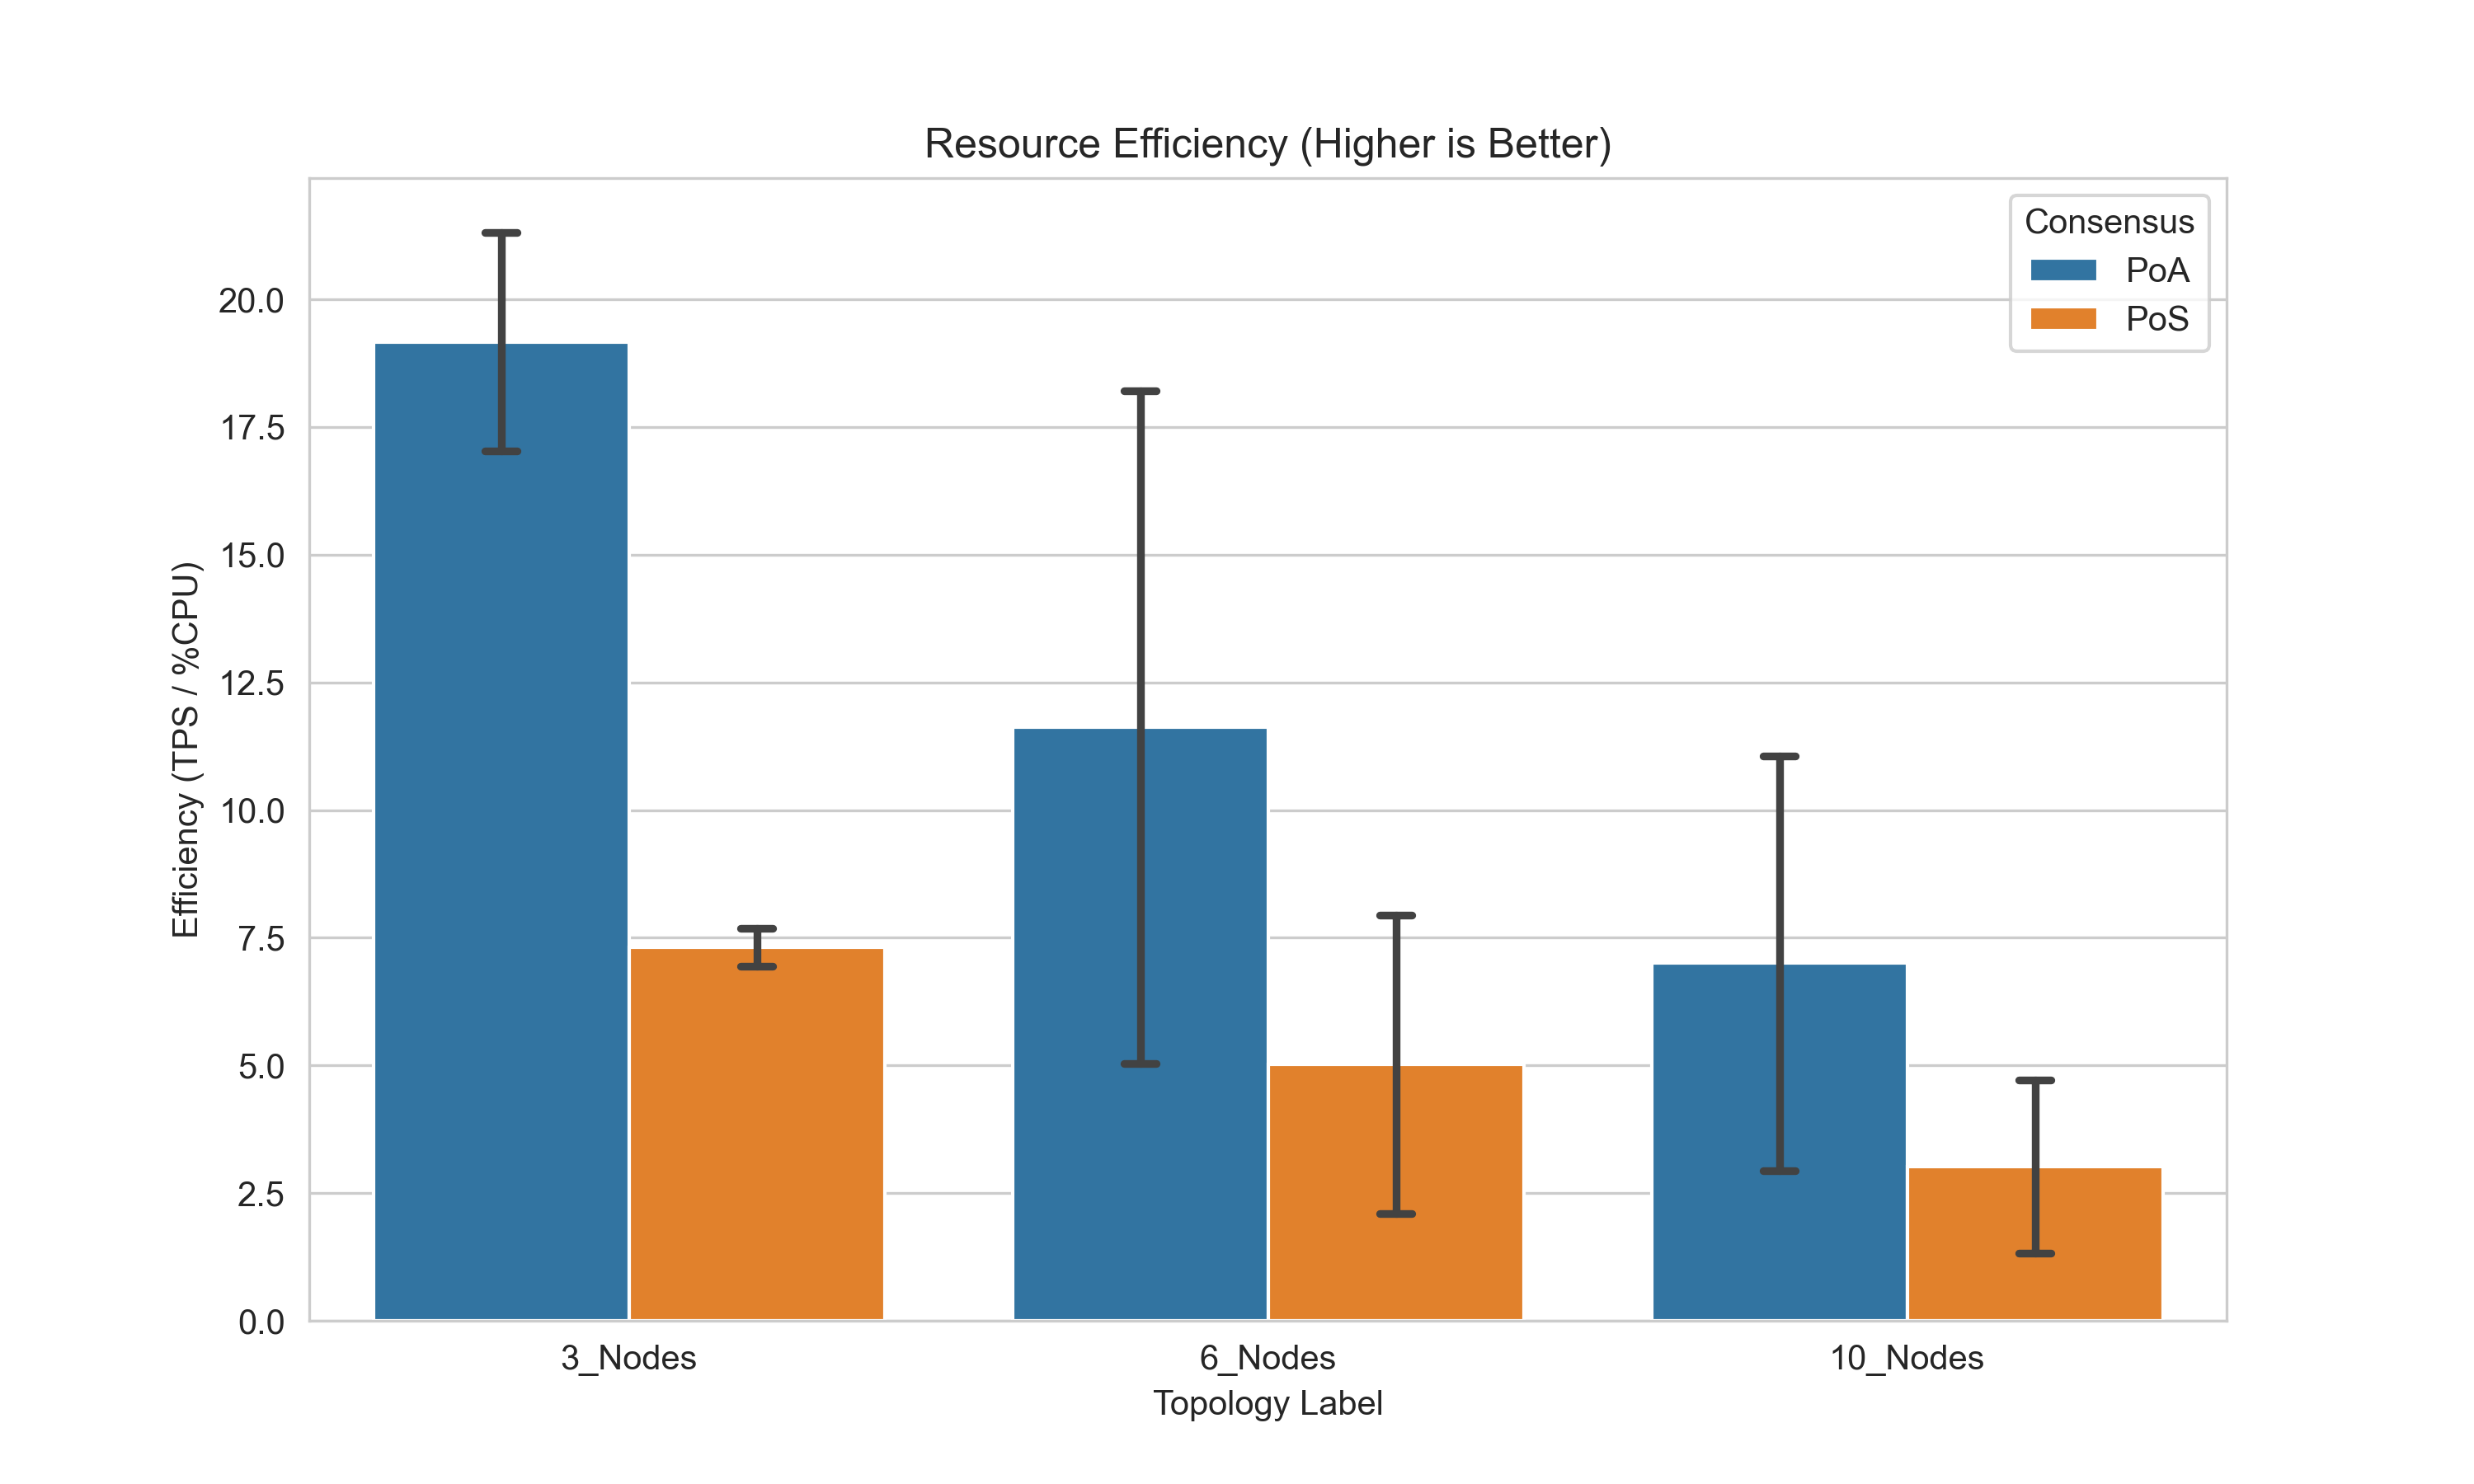
\includegraphics[width=0.9\textwidth]{images/efficiency_resource_cpu.png}
    \caption{Efisiensi Sumber Daya (TPS per \% CPU)}
    \label{fig:efficiency_cpu}
\end{figure}

\begin{figure}[htbp]
    \centering
    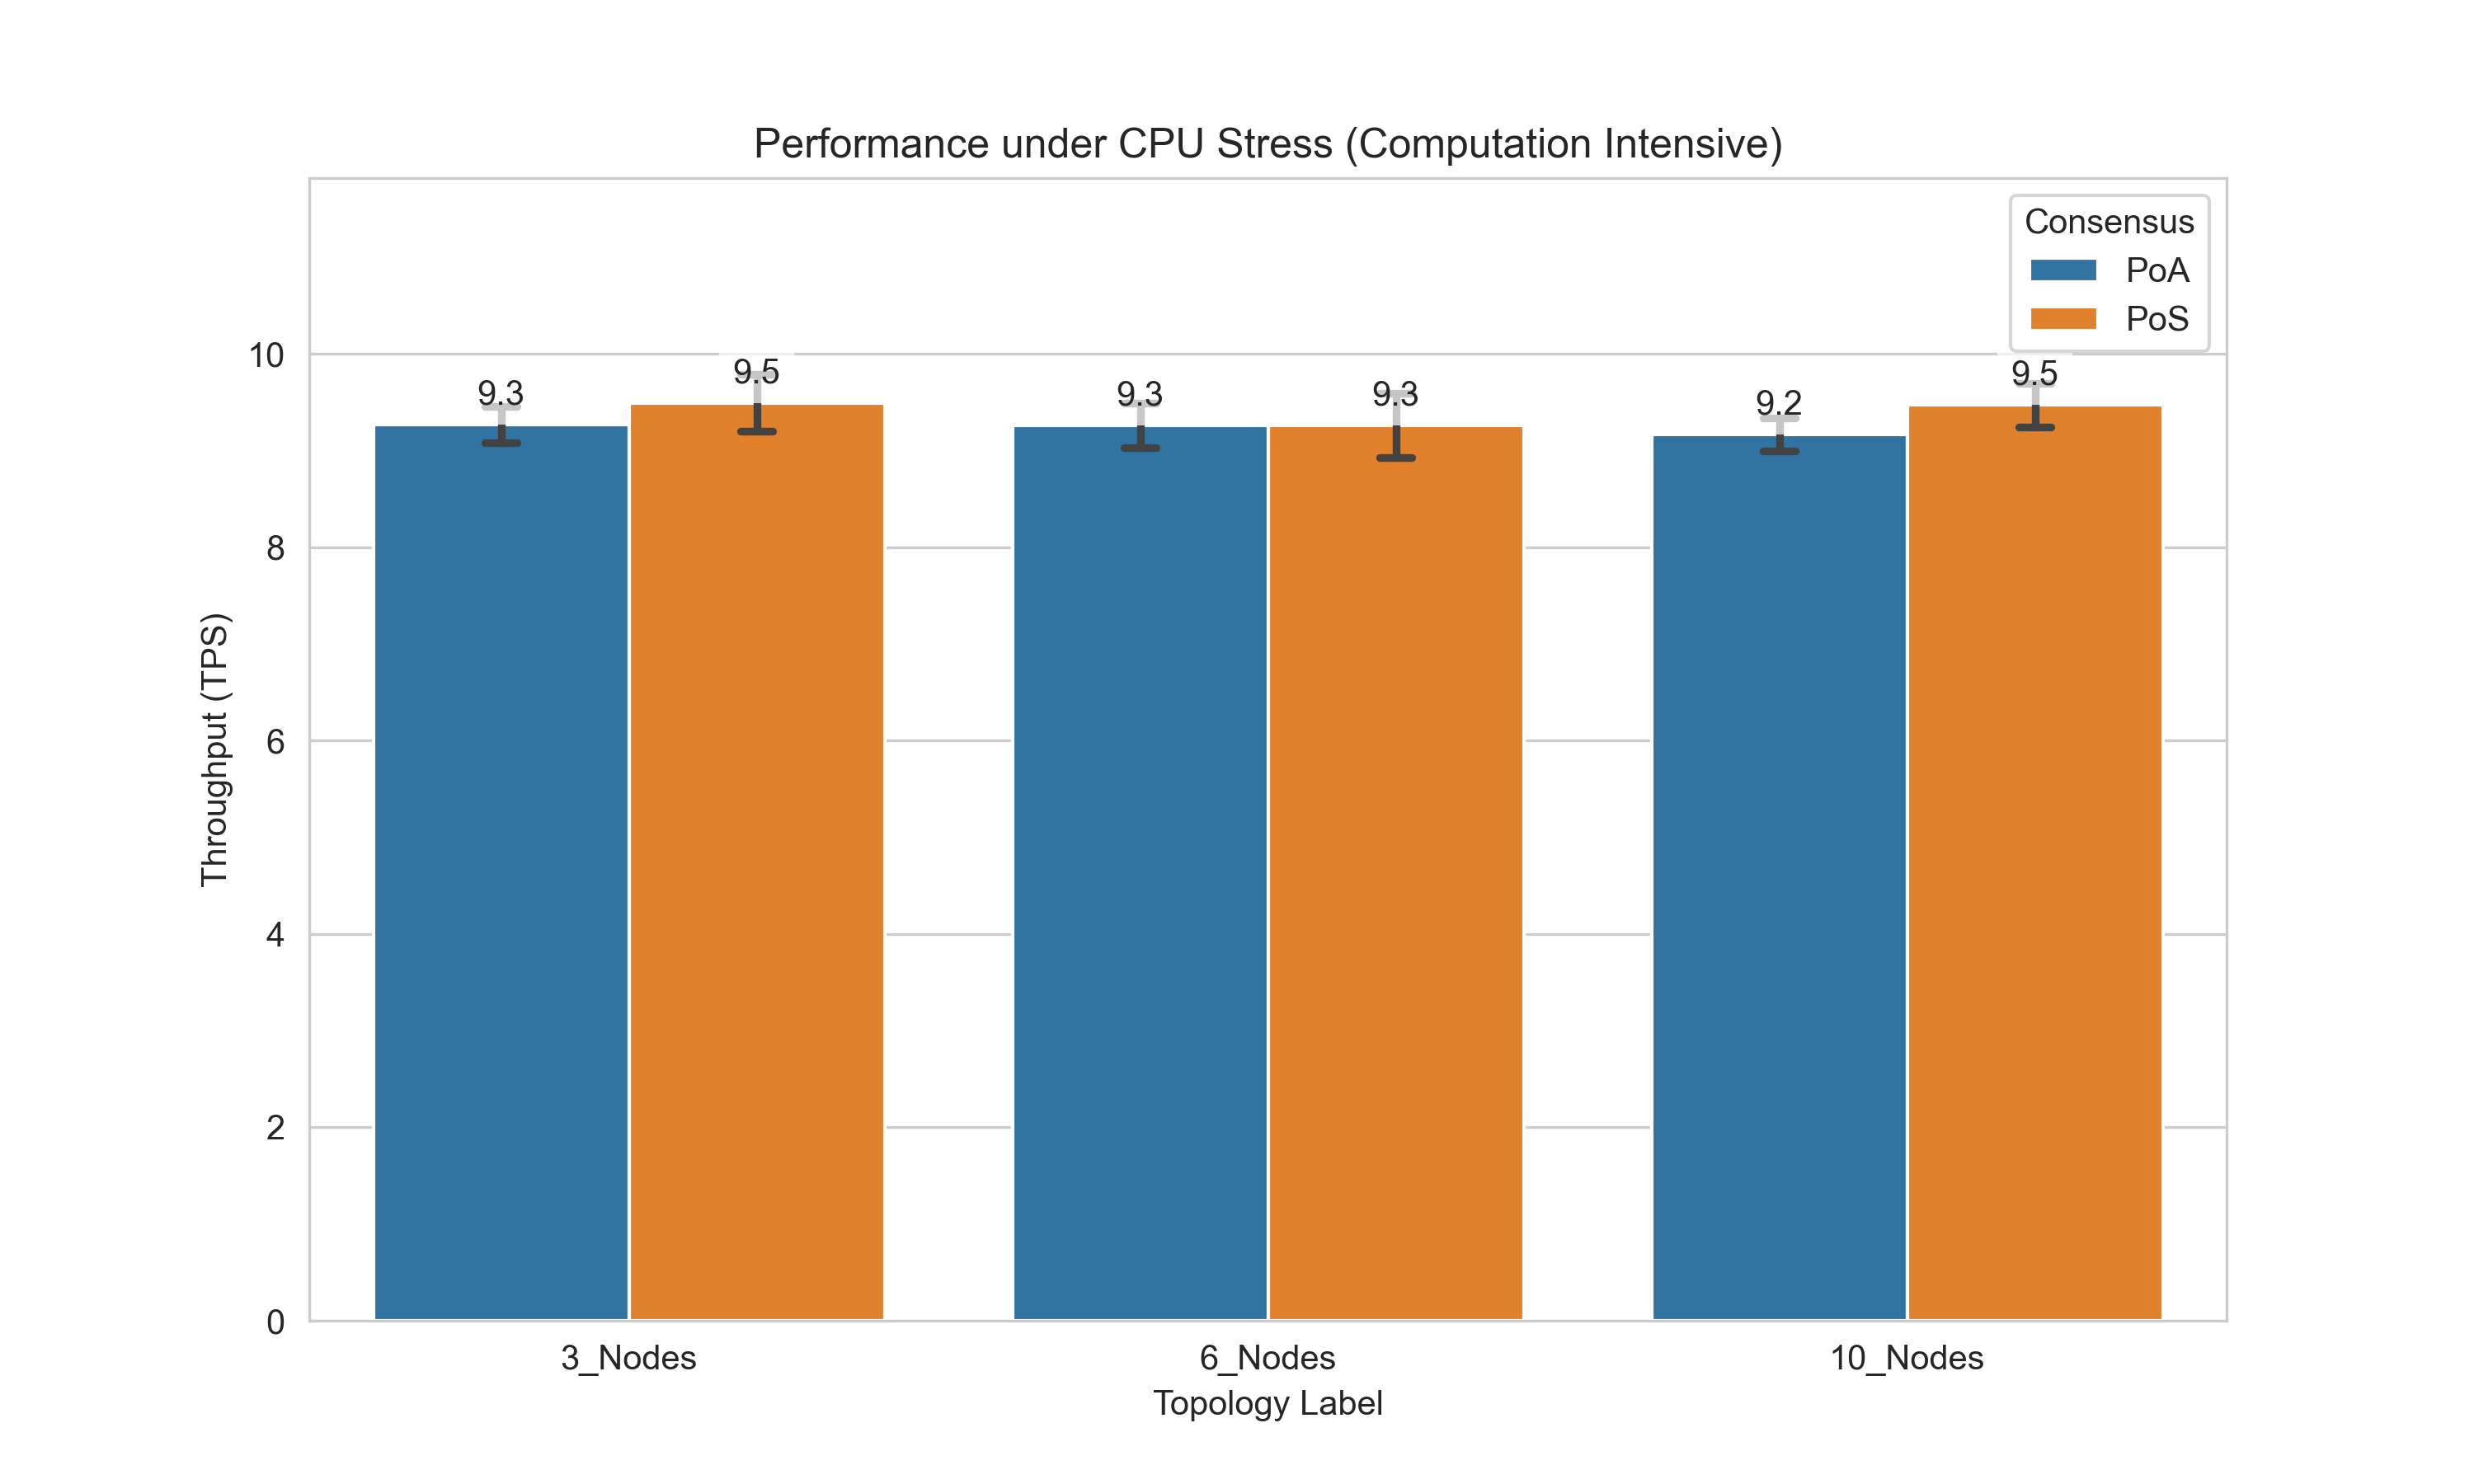
\includegraphics[width=0.9\textwidth]{images/cpu_stress_comparison.png}
    \caption{Perbandingan CPU Stress Test}
    \label{fig:cpu_stress}
\end{figure}

\begin{figure}[htbp]
    \centering
    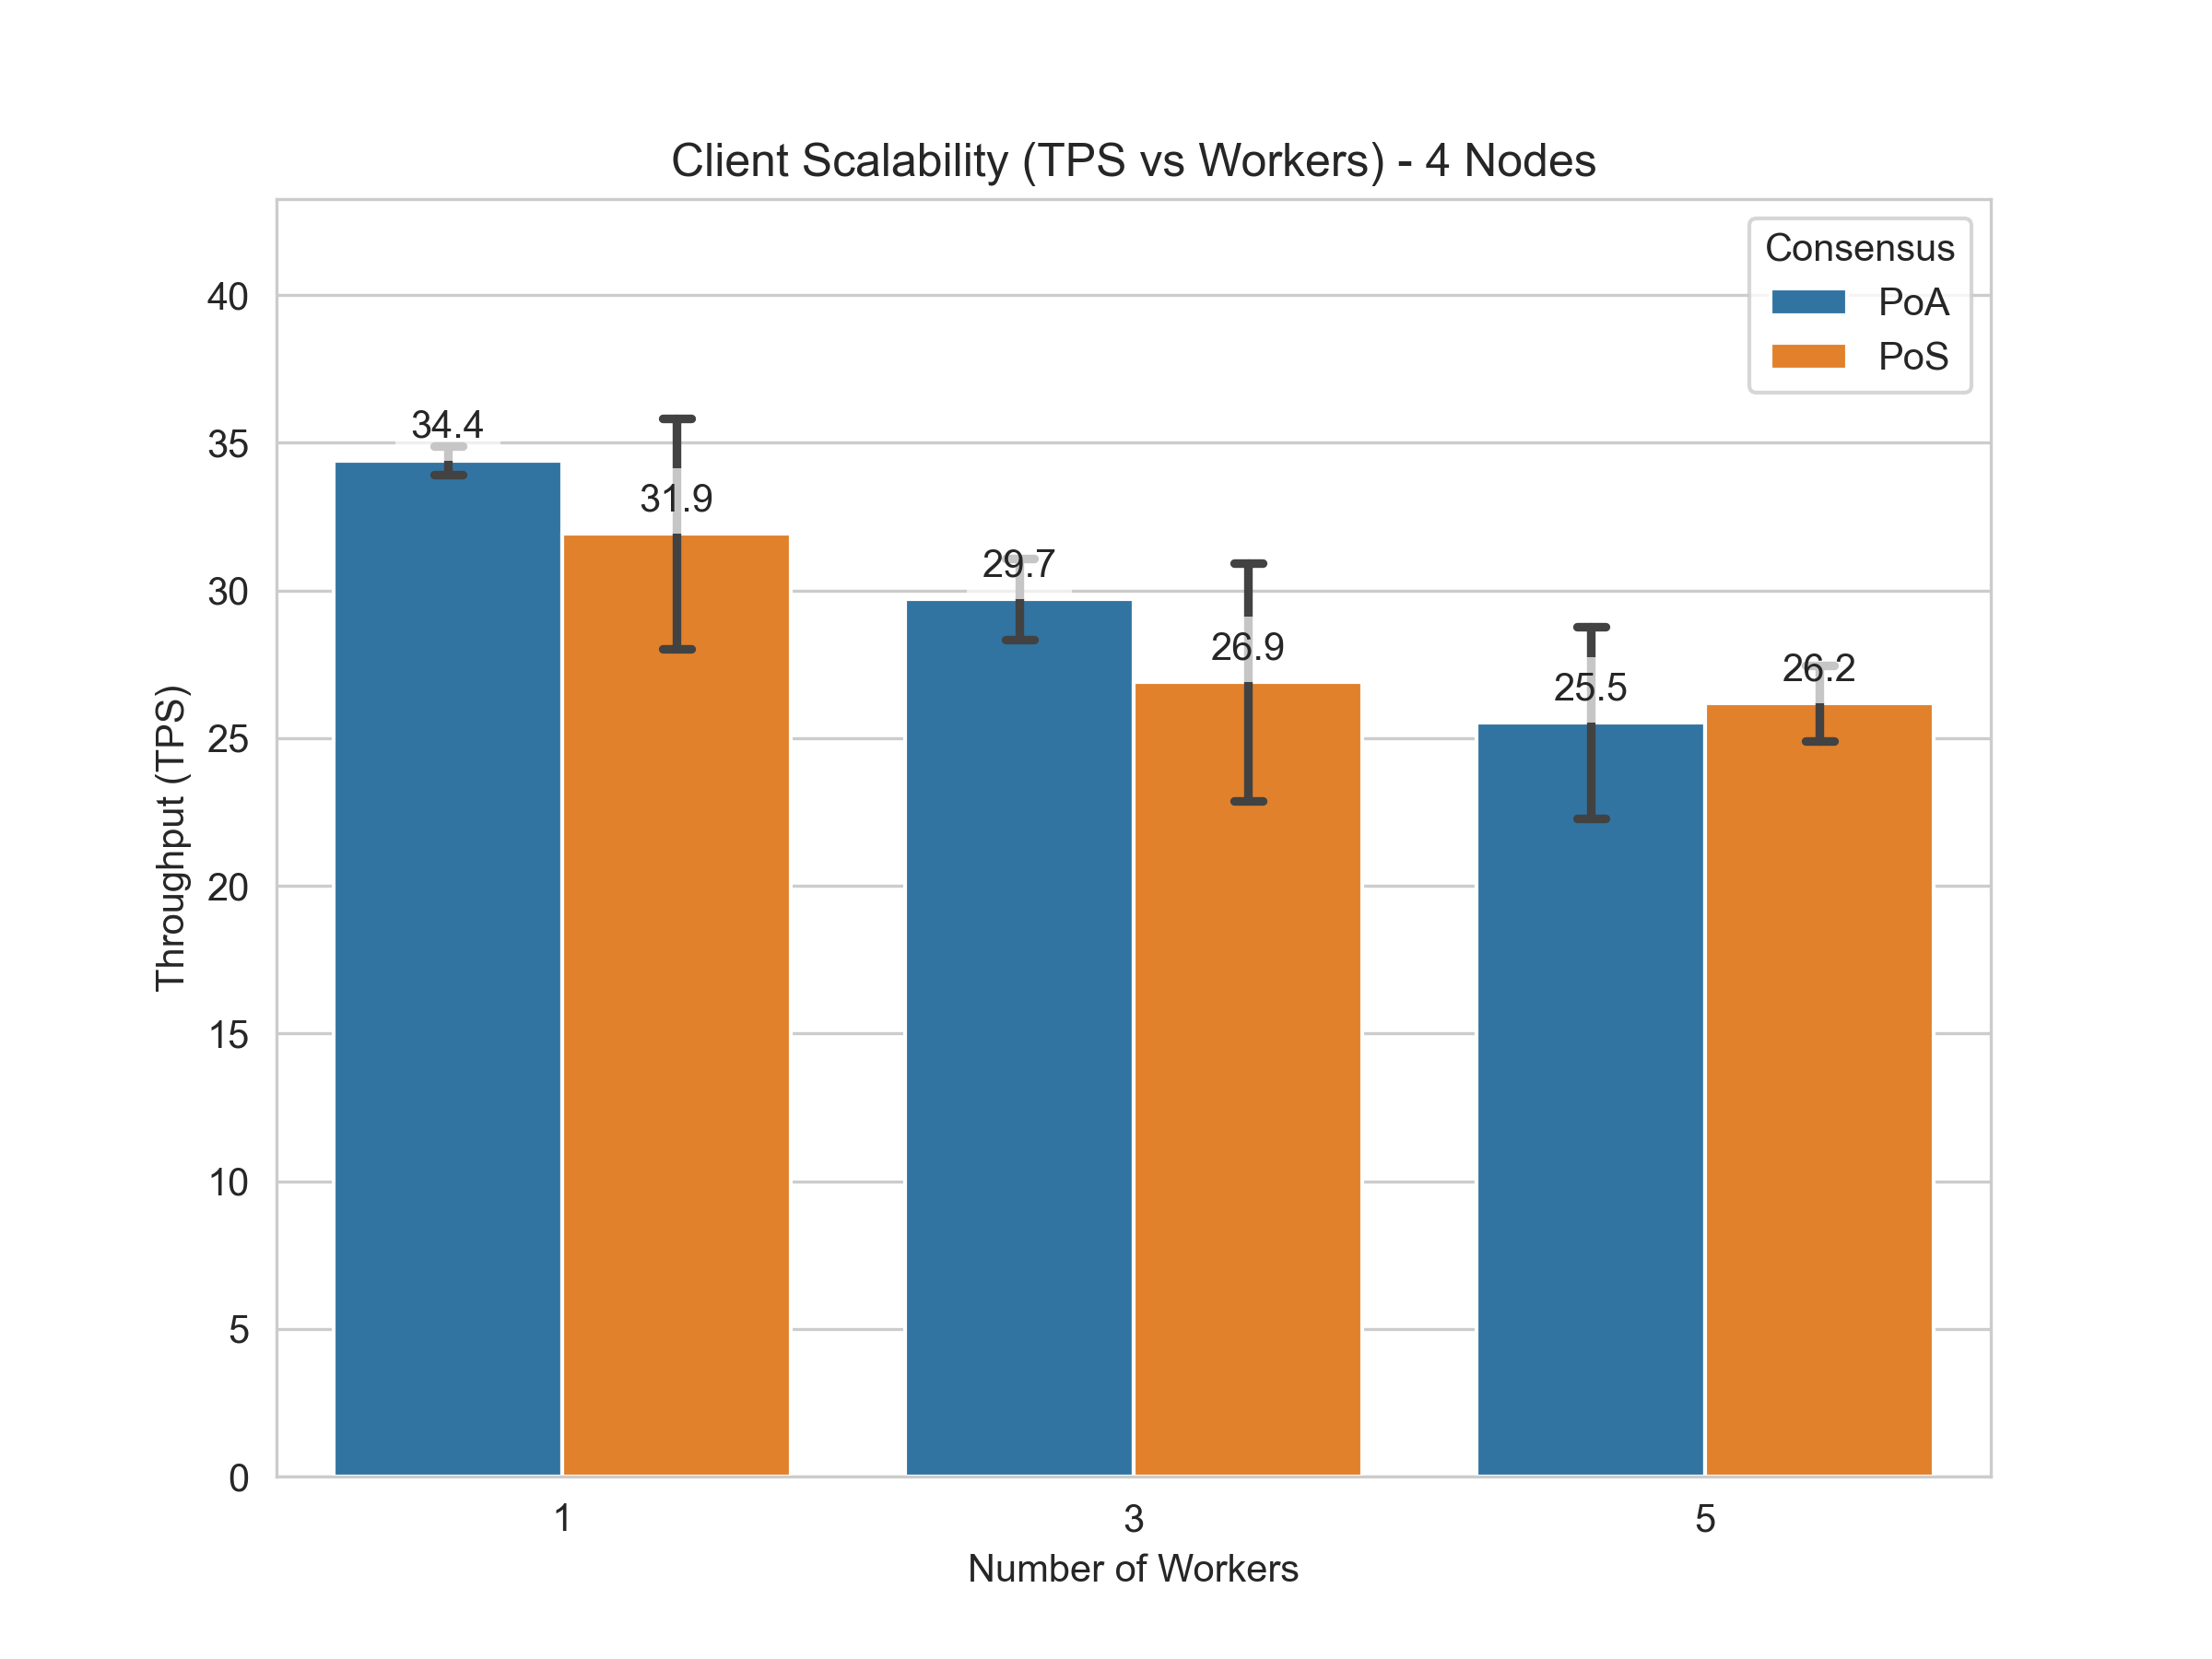
\includegraphics[width=0.9\textwidth]{images/scalability_client_tps_4_Nodes.png}
    \caption{Skalabilitas Klien pada Topologi 4 Node}
    \label{fig:scalability_client_4}
\end{figure}

\begin{figure}[htbp]
    \centering
    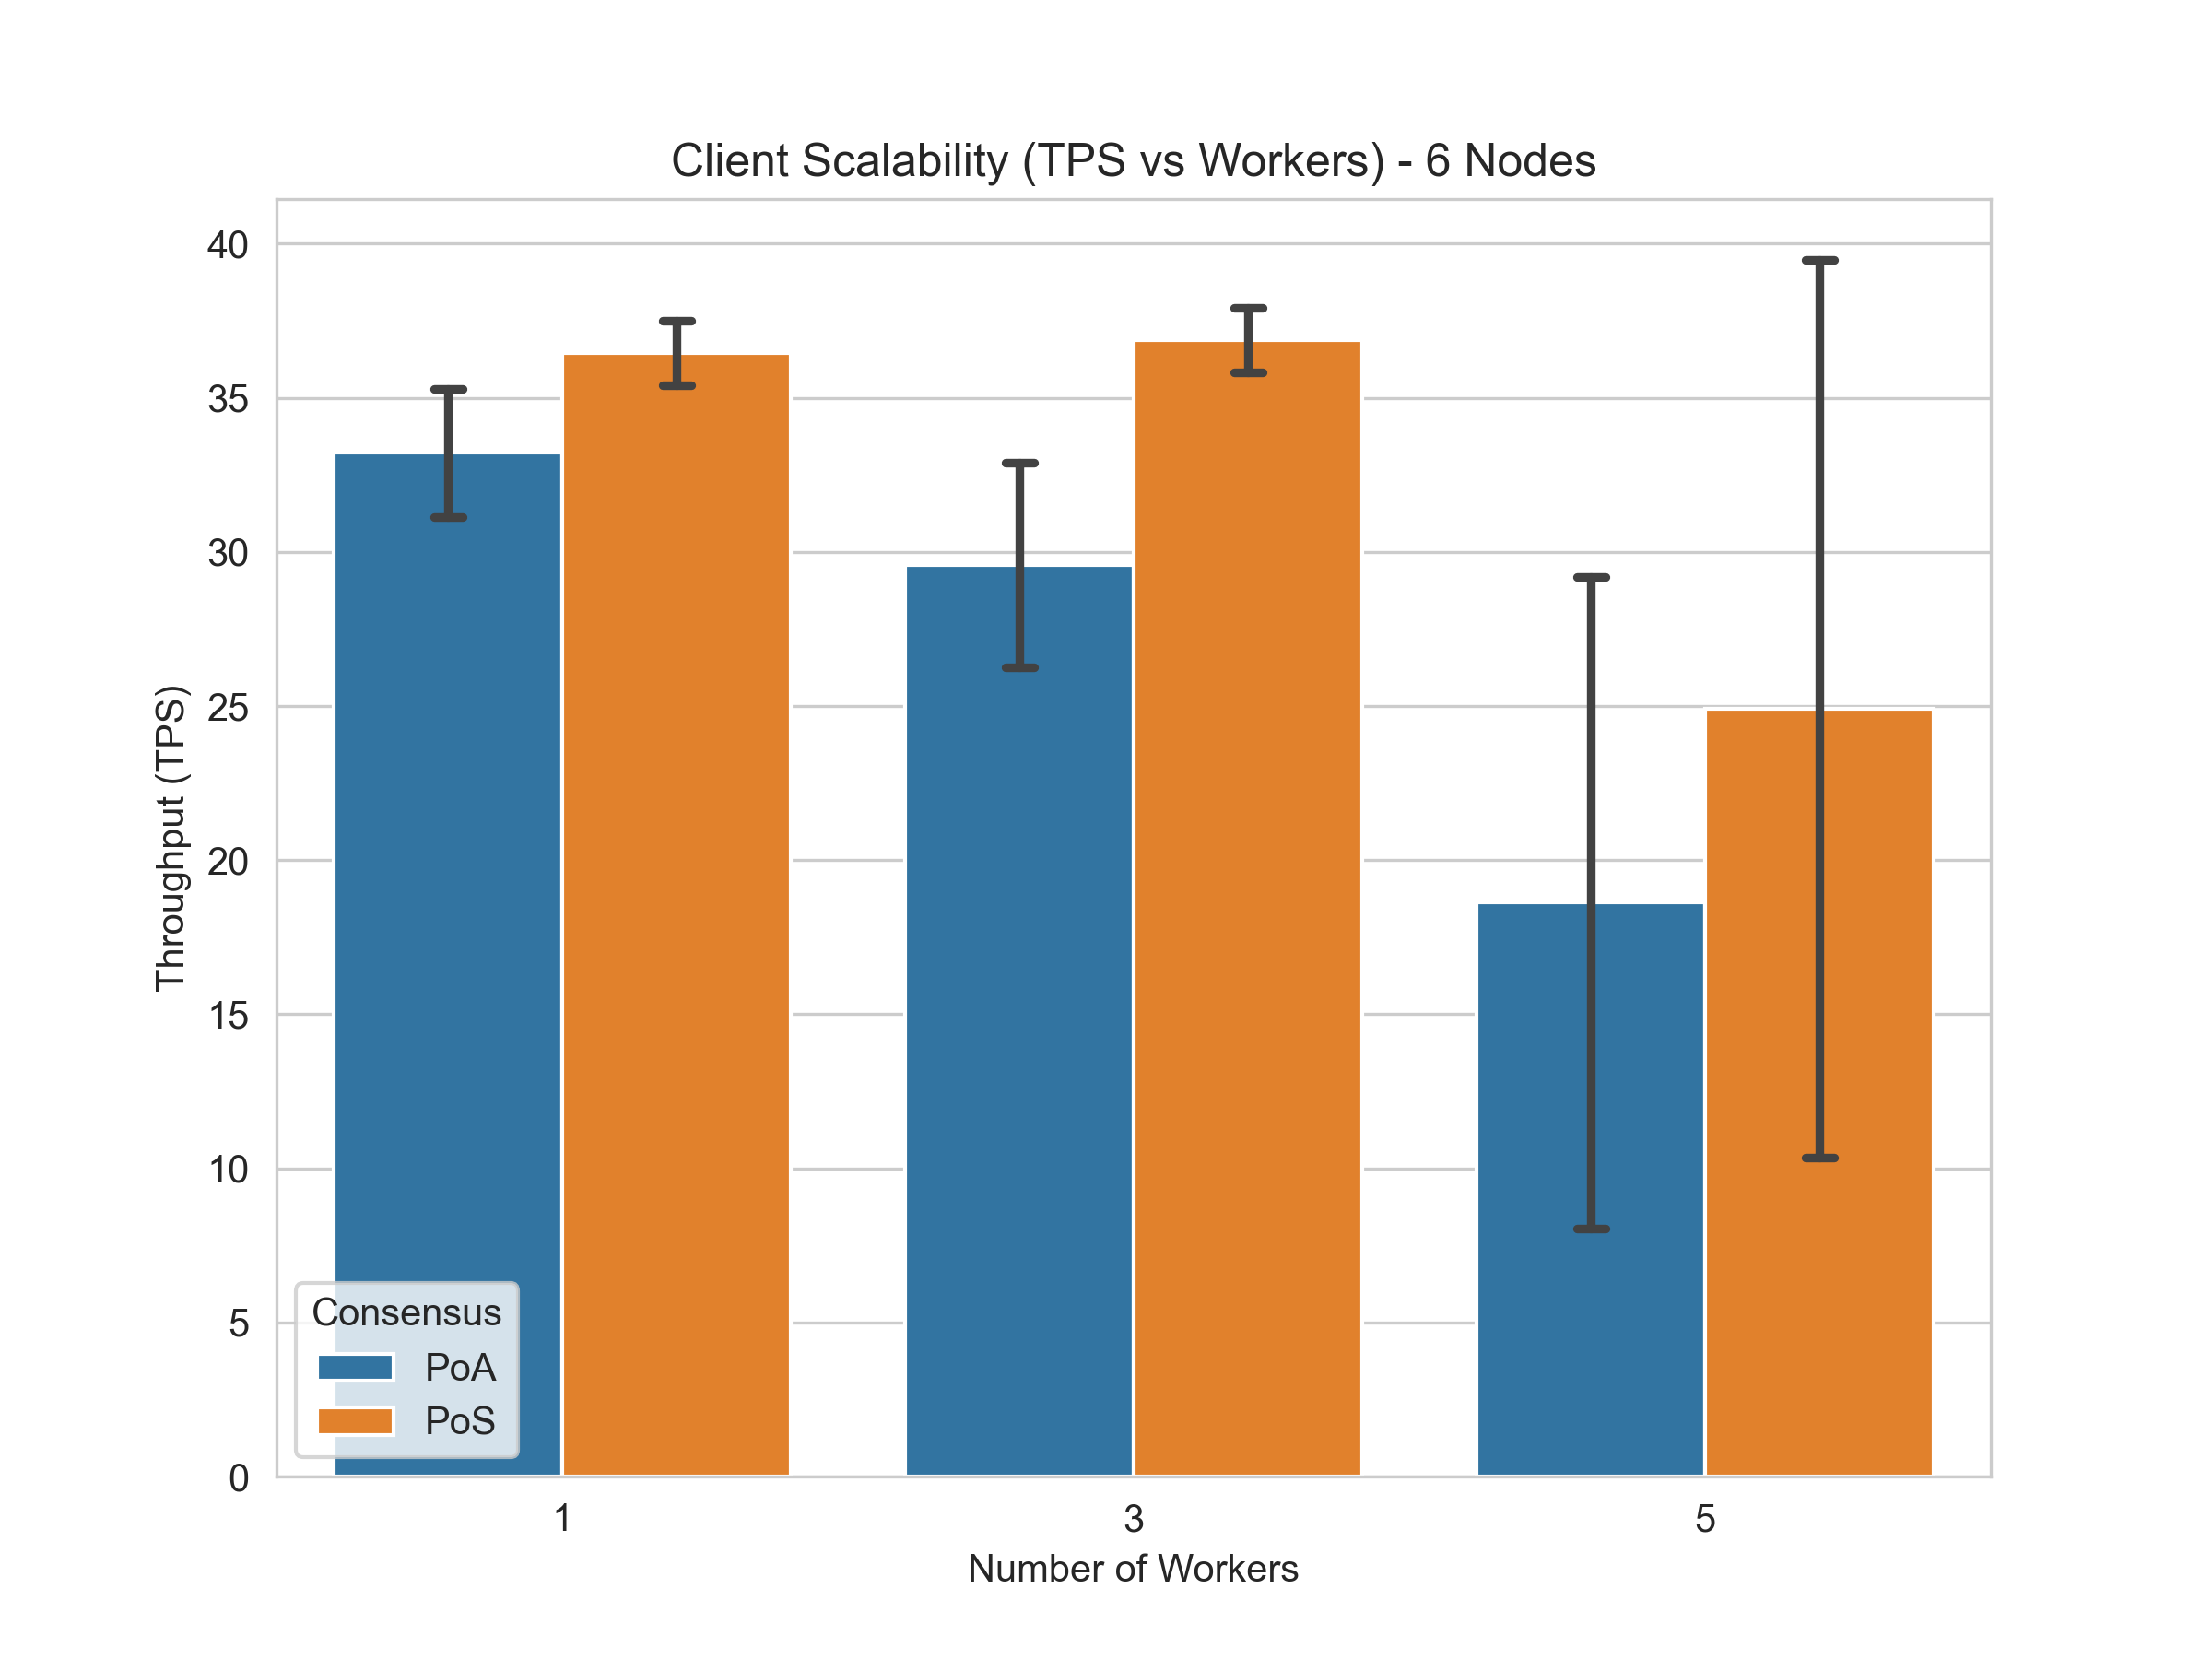
\includegraphics[width=0.9\textwidth]{images/scalability_client_tps_6_Nodes.png}
    \caption{Skalabilitas Klien pada Topologi 6 Node}
    \label{fig:scalability_client_6}
\end{figure}

\begin{figure}[htbp]
    \centering
    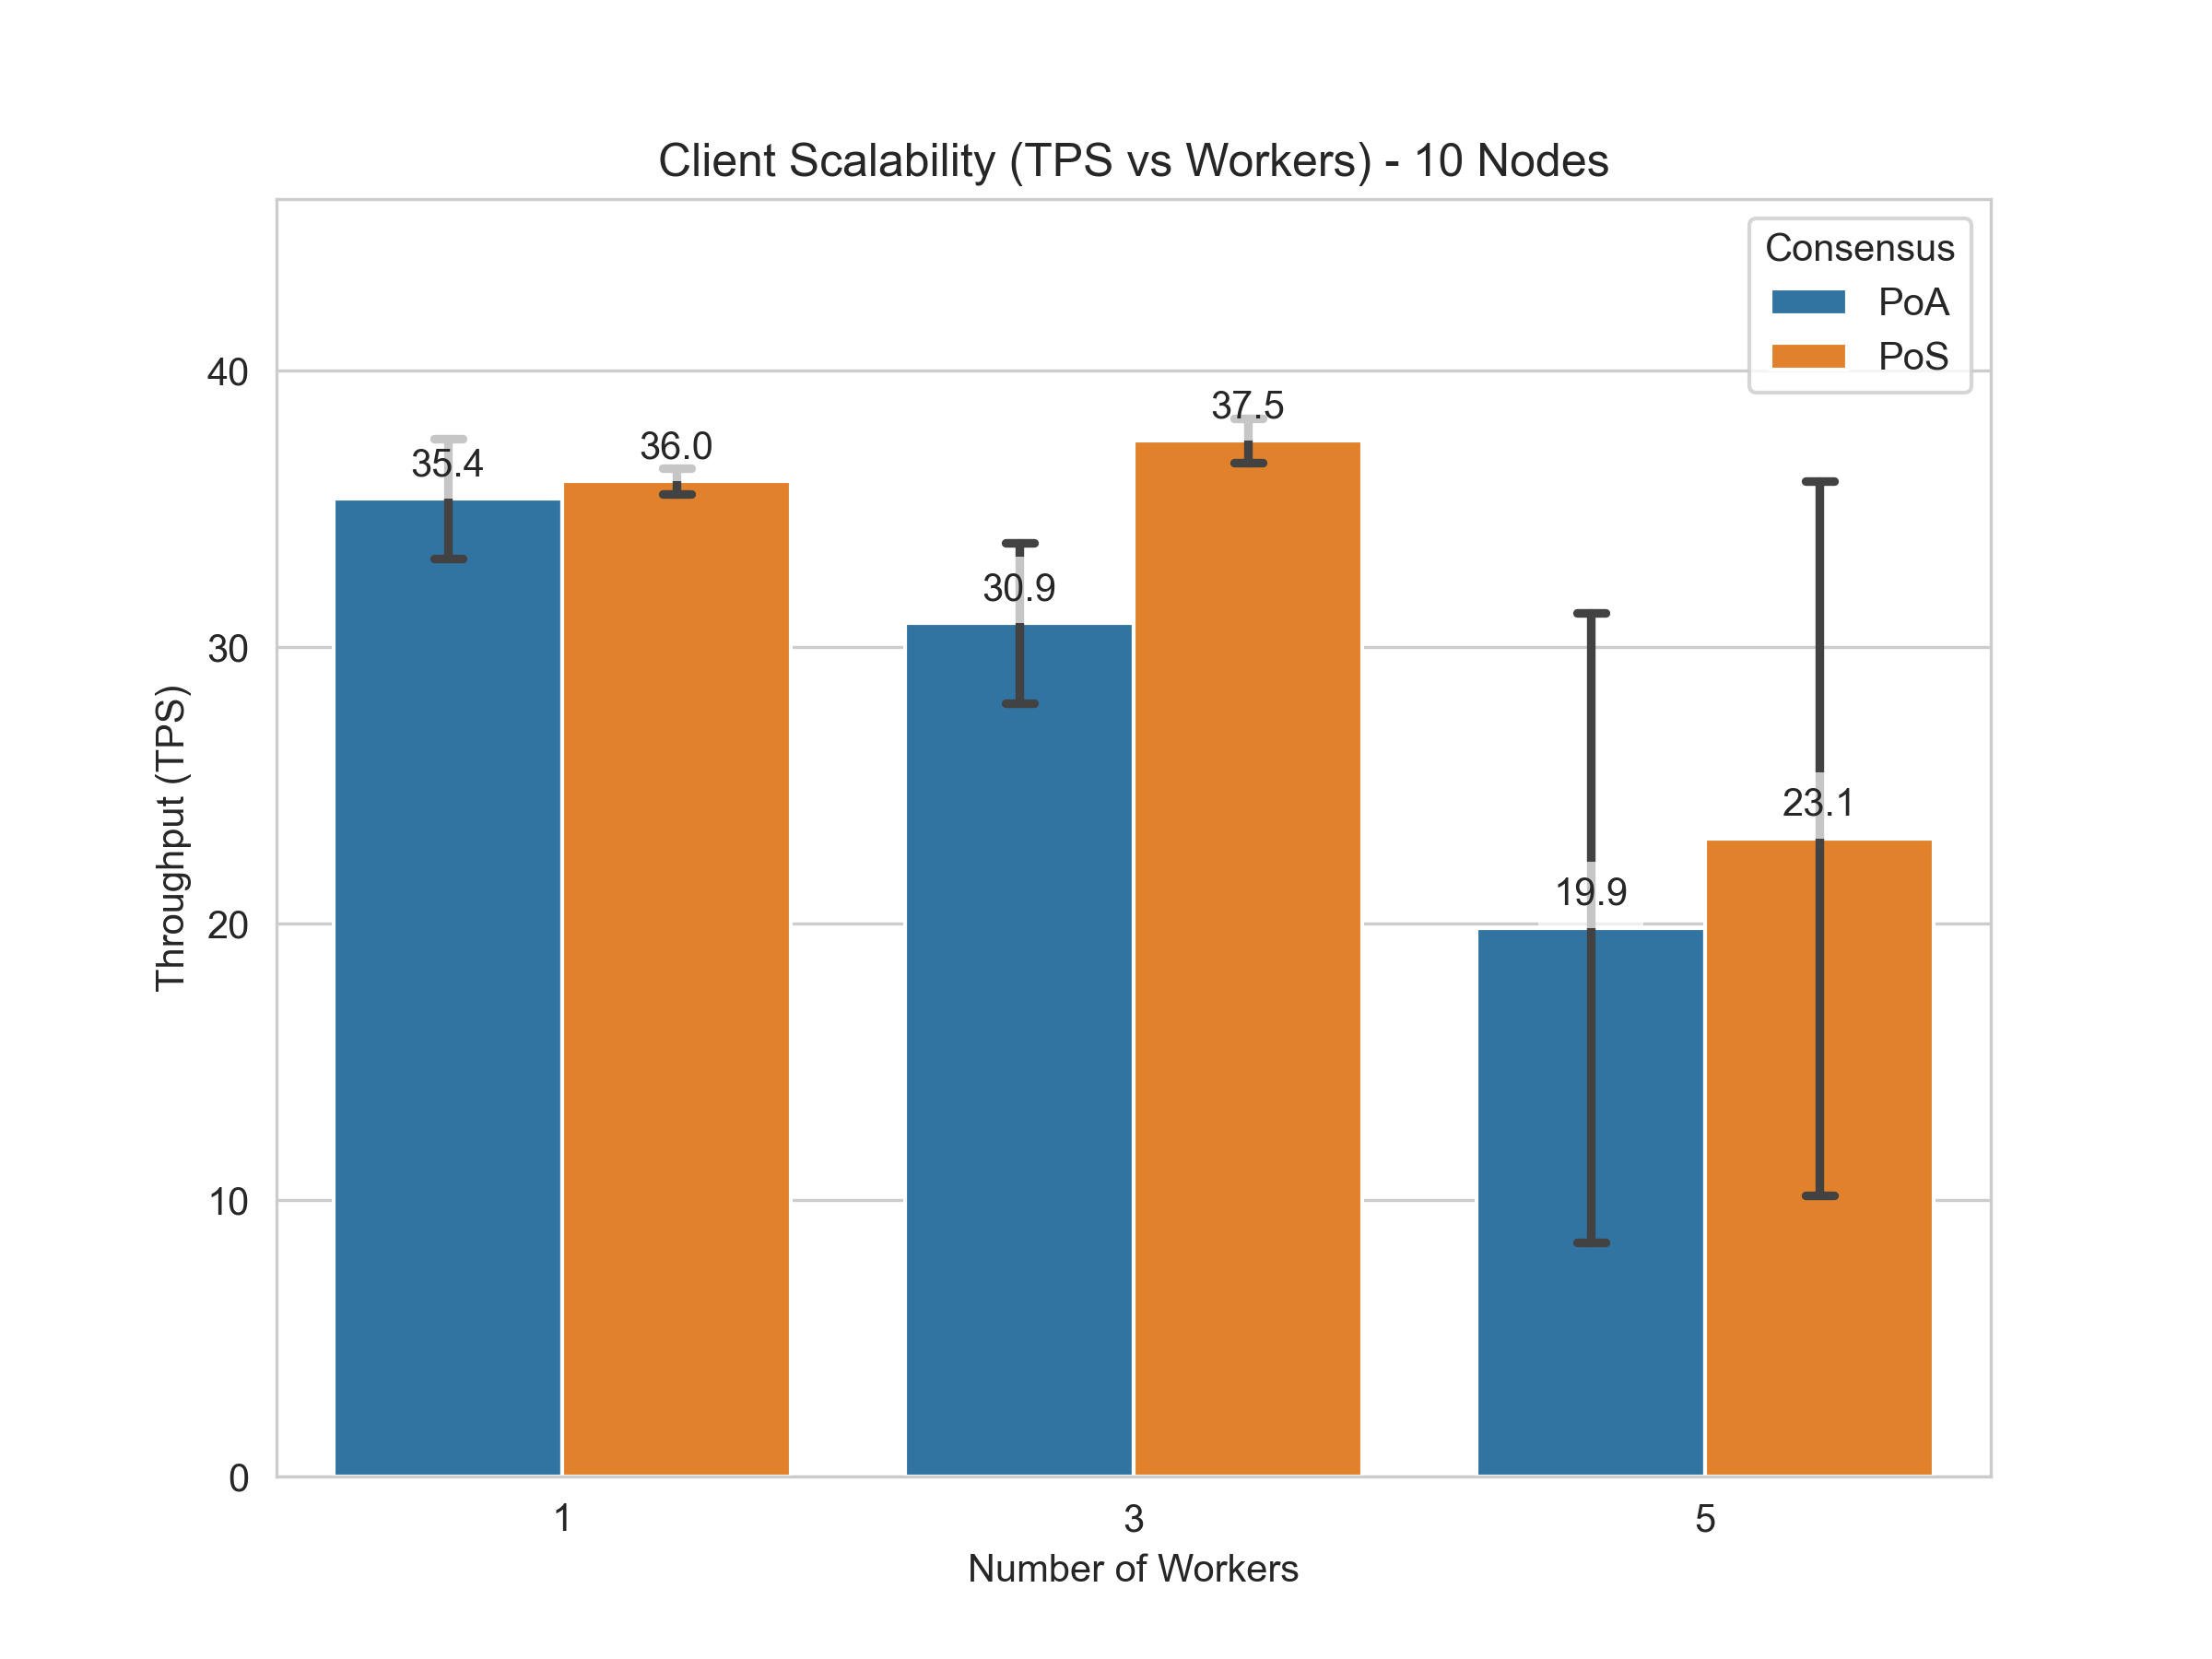
\includegraphics[width=0.9\textwidth]{images/scalability_client_tps_10_Nodes.png}
    \caption{Skalabilitas Klien pada Topologi 10 Node}
    \label{fig:scalability_client_10}
\end{figure}

\subsection{Stabilitas Jaringan (Soak Test)}

Uji durabilitas (\textit{Soak Test}) selama 15 menit dilakukan untuk memverifikasi kestabilan jaringan. Hasilnya dapat dilihat pada grafik \textit{Time Series} TPS (Gambar \ref{fig:stability_timeseries_tps_4}, \ref{fig:stability_timeseries_tps_6}, \ref{fig:stability_timeseries_tps_10}).

Garis yang mendatar (flat) pada grafik time-series TPS menunjukkan stabilitas yang sangat baik. Hal serupa juga terlihat pada stabilitas latensi (Gambar \ref{fig:stability_timeseries_latency_4}, \ref{fig:stability_timeseries_latency_6}, \ref{fig:stability_timeseries_latency_10}), di mana waktu respons tetap konsisten sepanjang pengujian tanpa adanya lonjakan (*spike*) yang tidak wajar. Baik PoA maupun PoS mampu mempertahankan performa yang konstan selama durasi pengujian.
Namun, jika dilihat dari Gambar \ref{fig:stability_cv} yang membandingkan \textit{Coefficient of Variation} (CV), PoA memiliki nilai CV yang sedikit lebih rendah di beberapa skenario, mengindikasikan variabilitas performa yang lebih kecil (lebih deterministik) dibandingkan PoS yang memiliki variasi probabilistik antar-blok.

\begin{figure}[htbp]
    \centering
    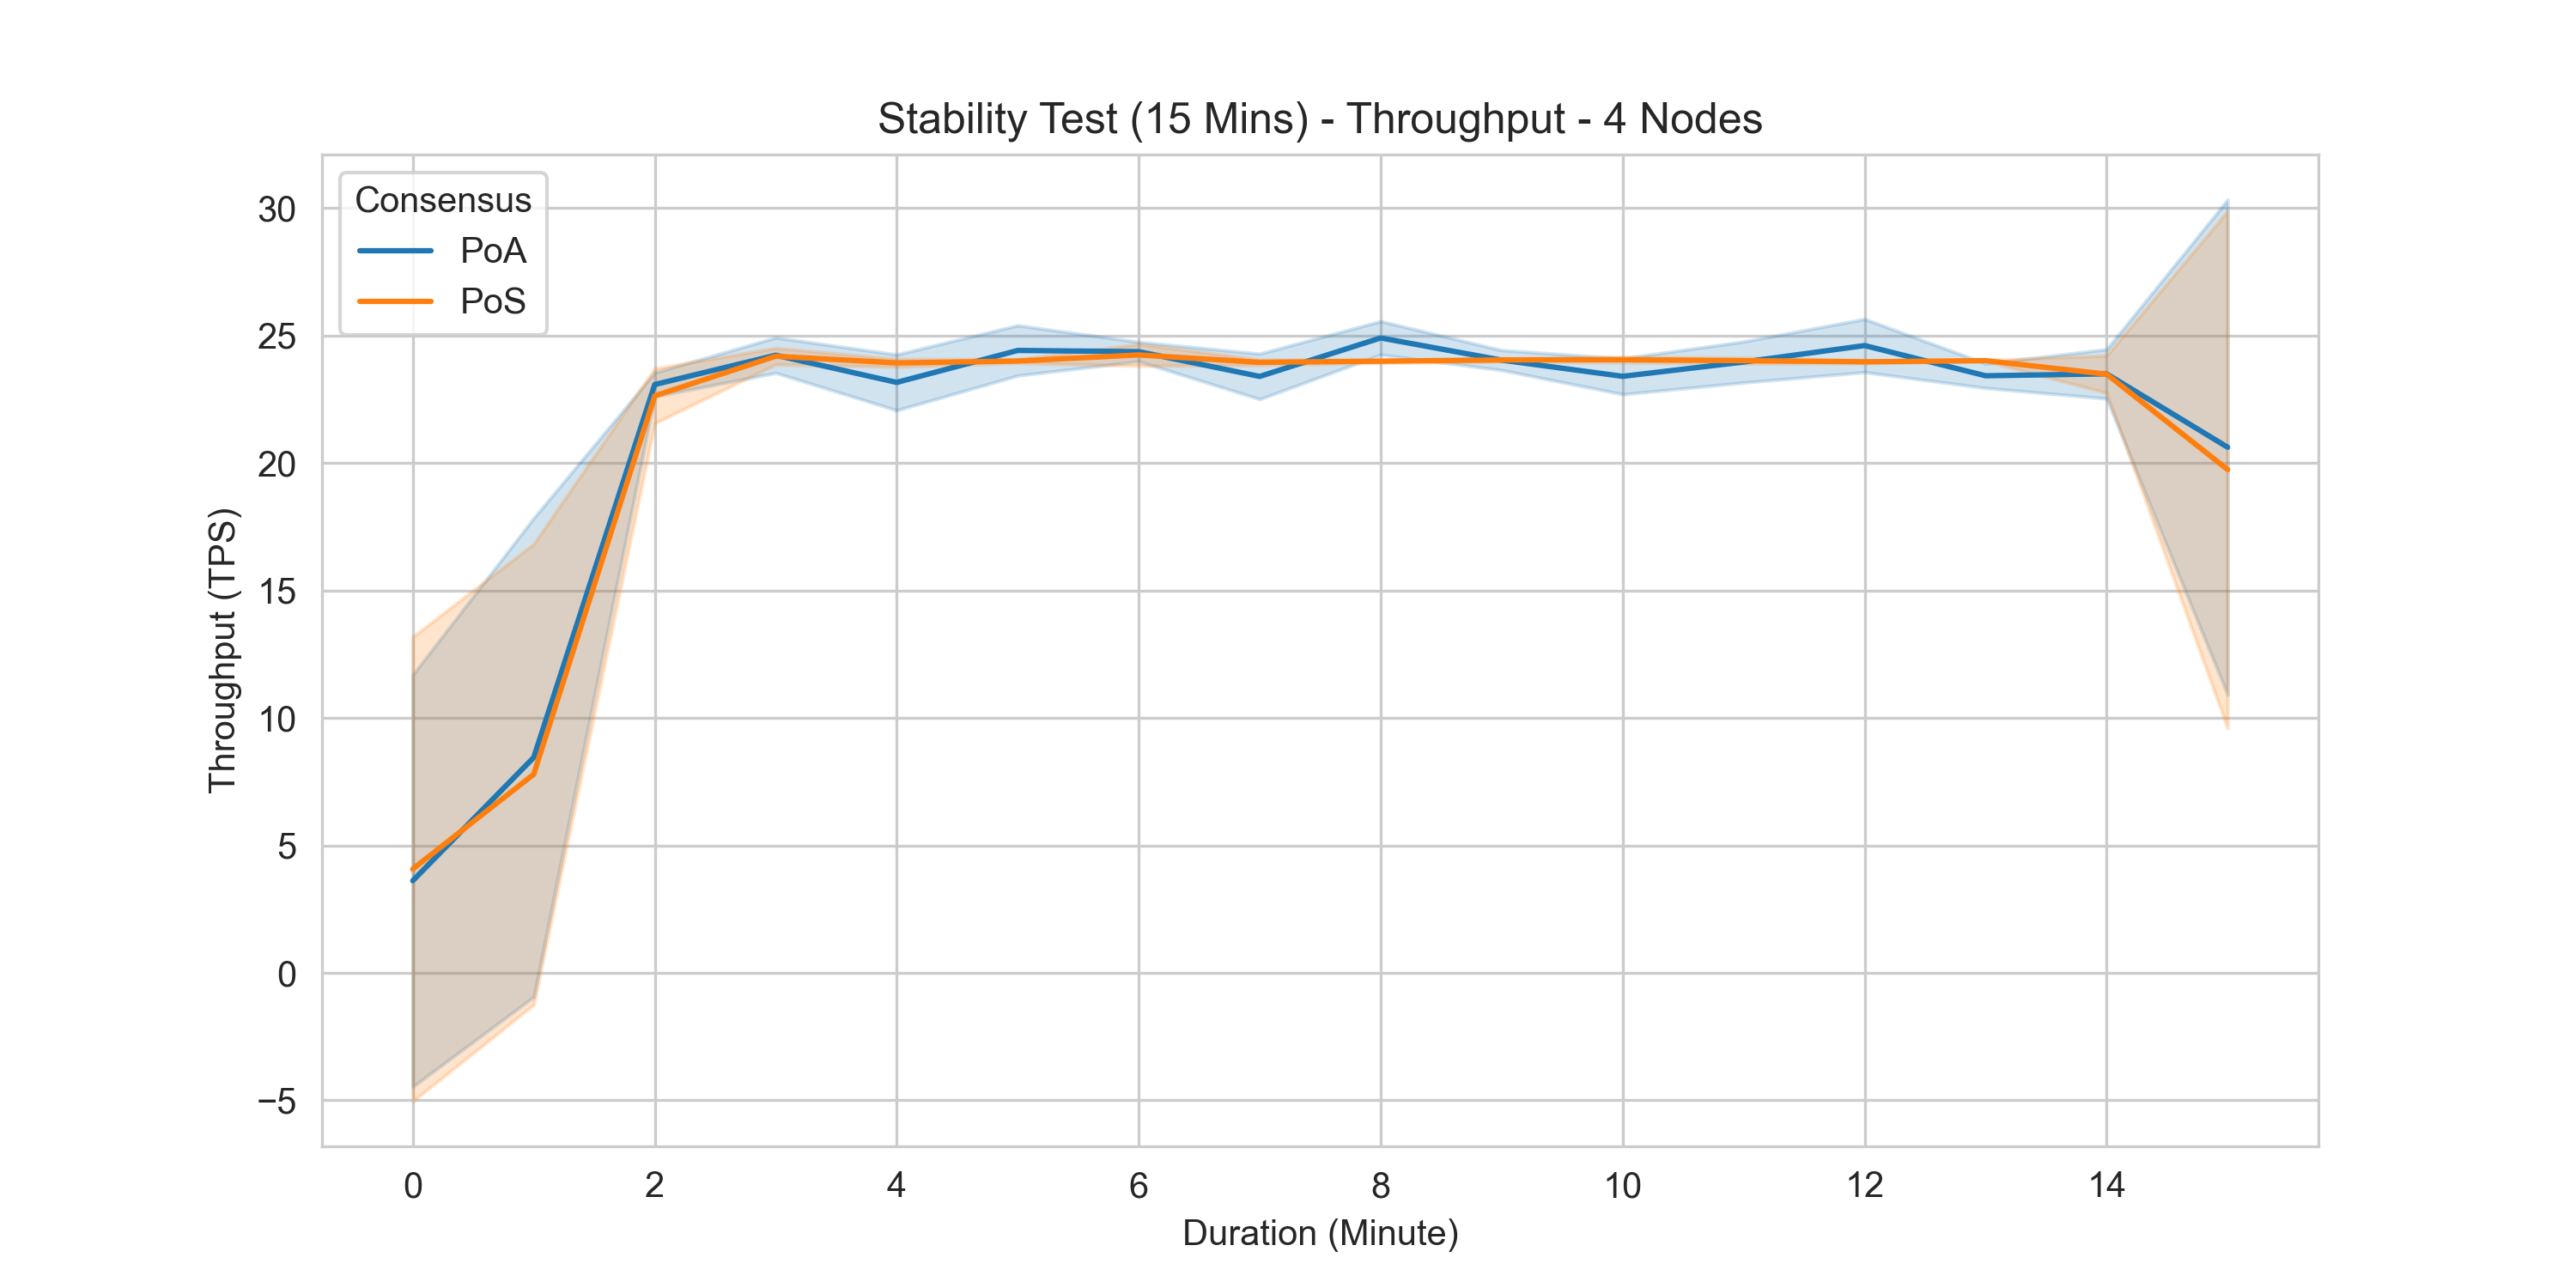
\includegraphics[width=0.9\textwidth]{images/stability_timeseries_tps_4_Nodes.png}
    \caption{Time Series TPS pada Uji Stabilitas (4 Node)}
    \label{fig:stability_timeseries_tps_4}
\end{figure}

\begin{figure}[htbp]
    \centering
    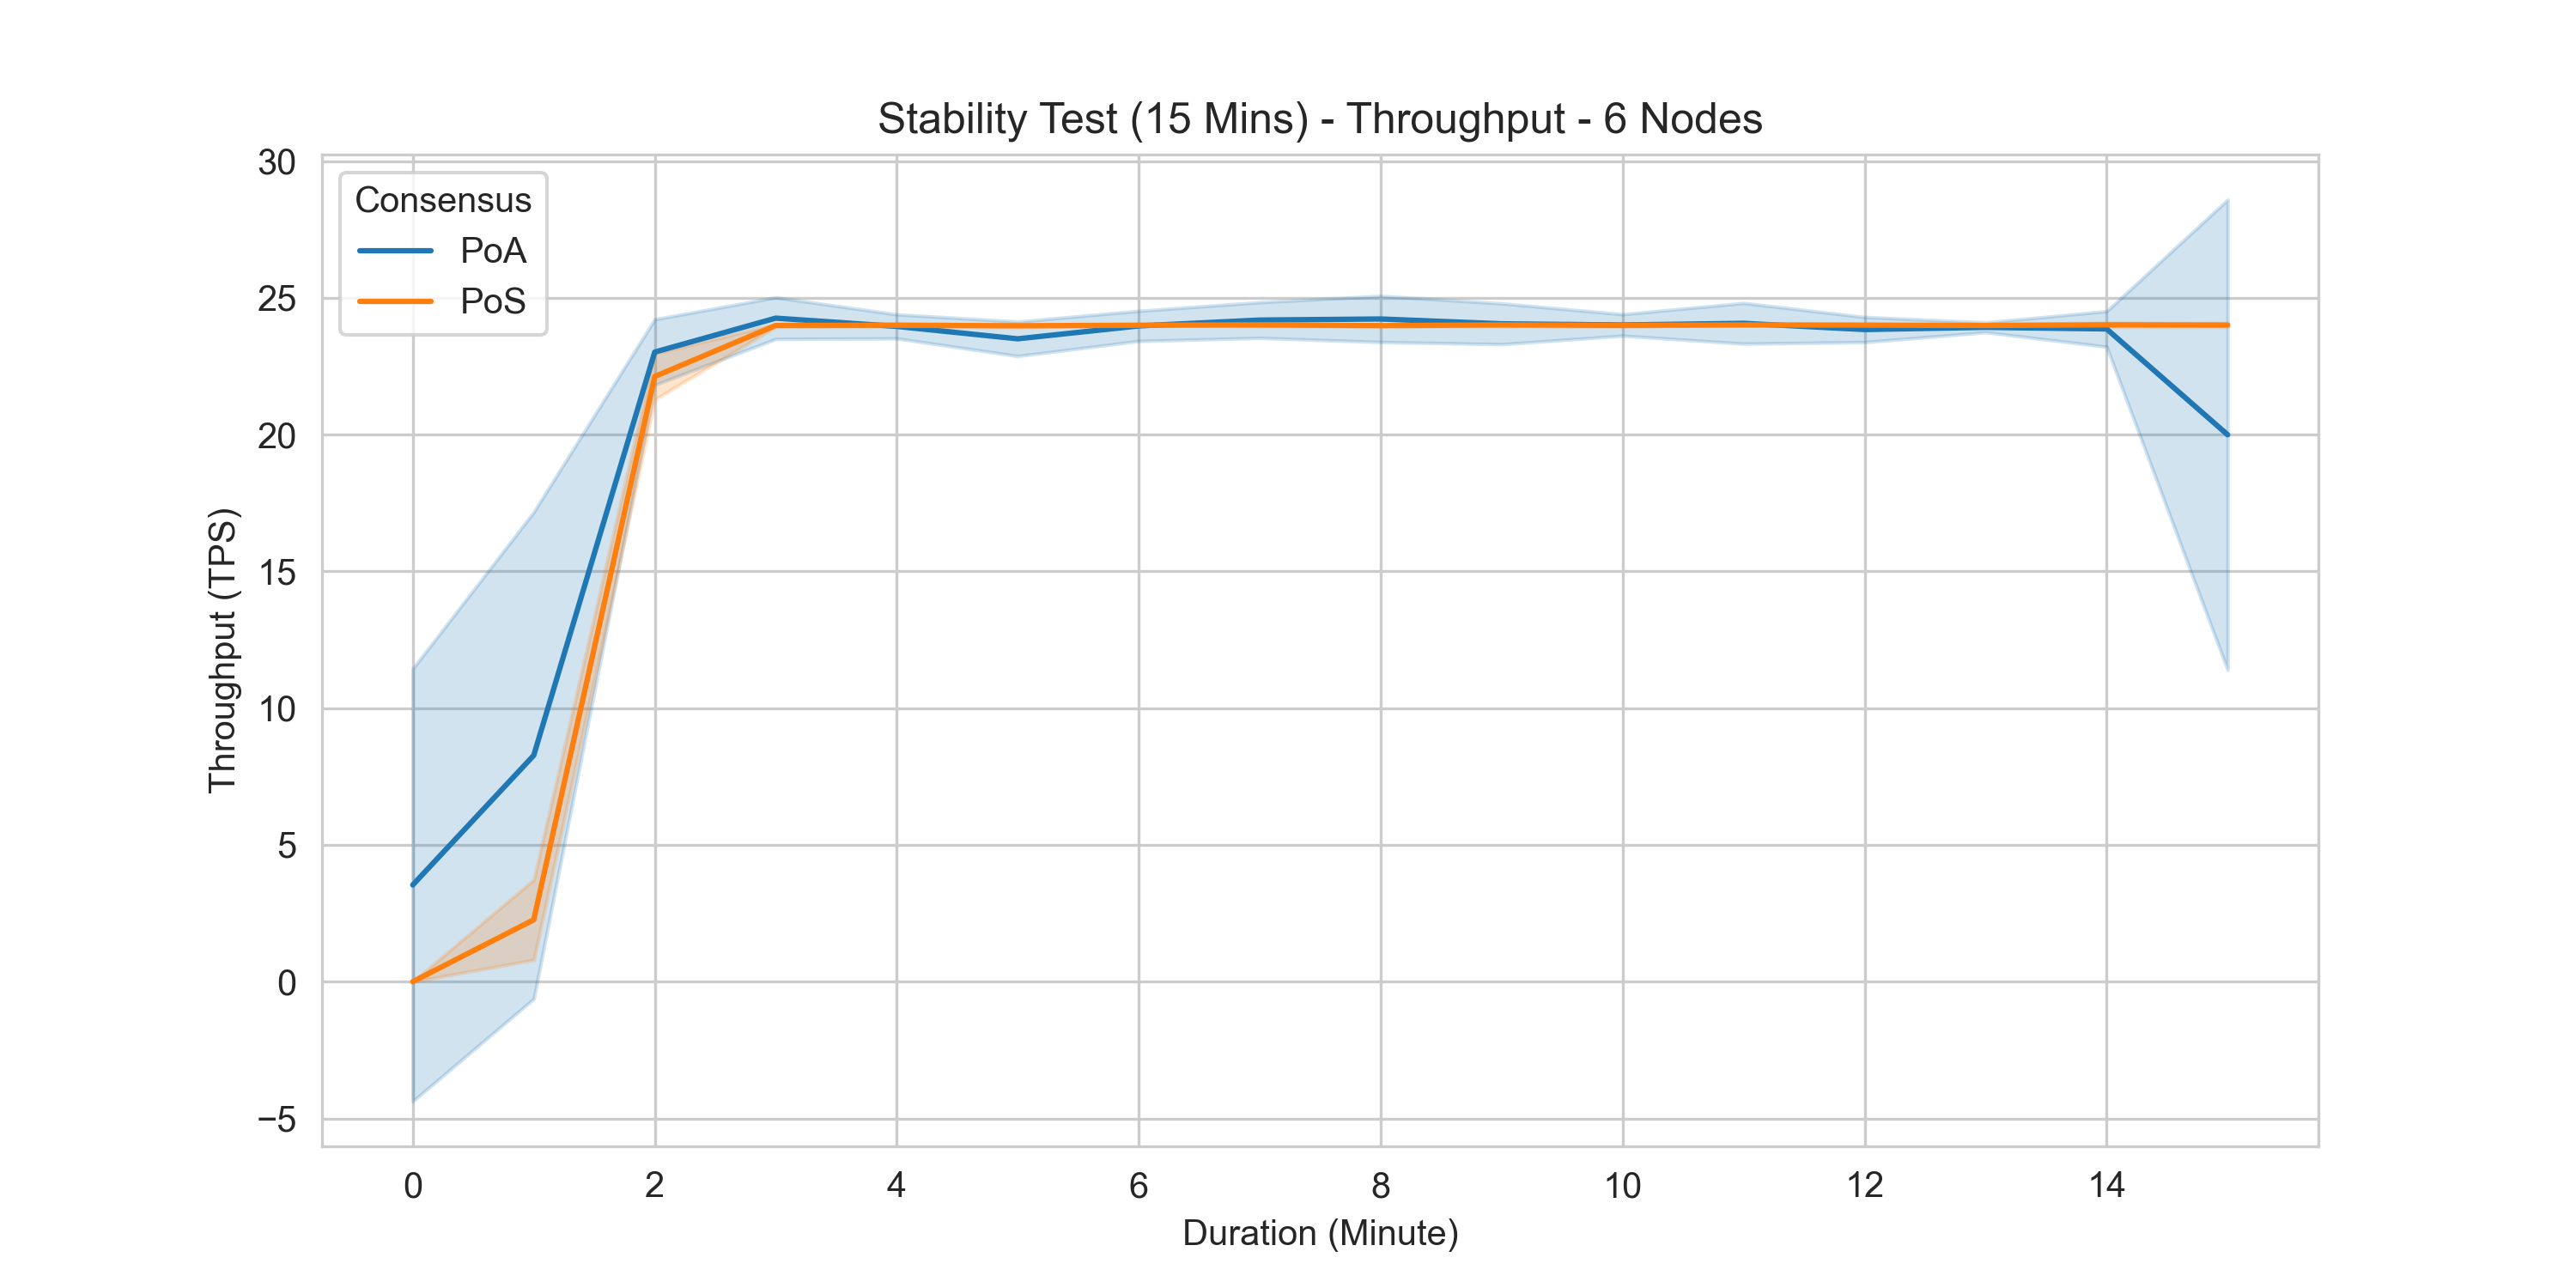
\includegraphics[width=0.9\textwidth]{images/stability_timeseries_tps_6_Nodes.png}
    \caption{Time Series TPS pada Uji Stabilitas (6 Node)}
    \label{fig:stability_timeseries_tps_6}
\end{figure}

\begin{figure}[htbp]
    \centering
    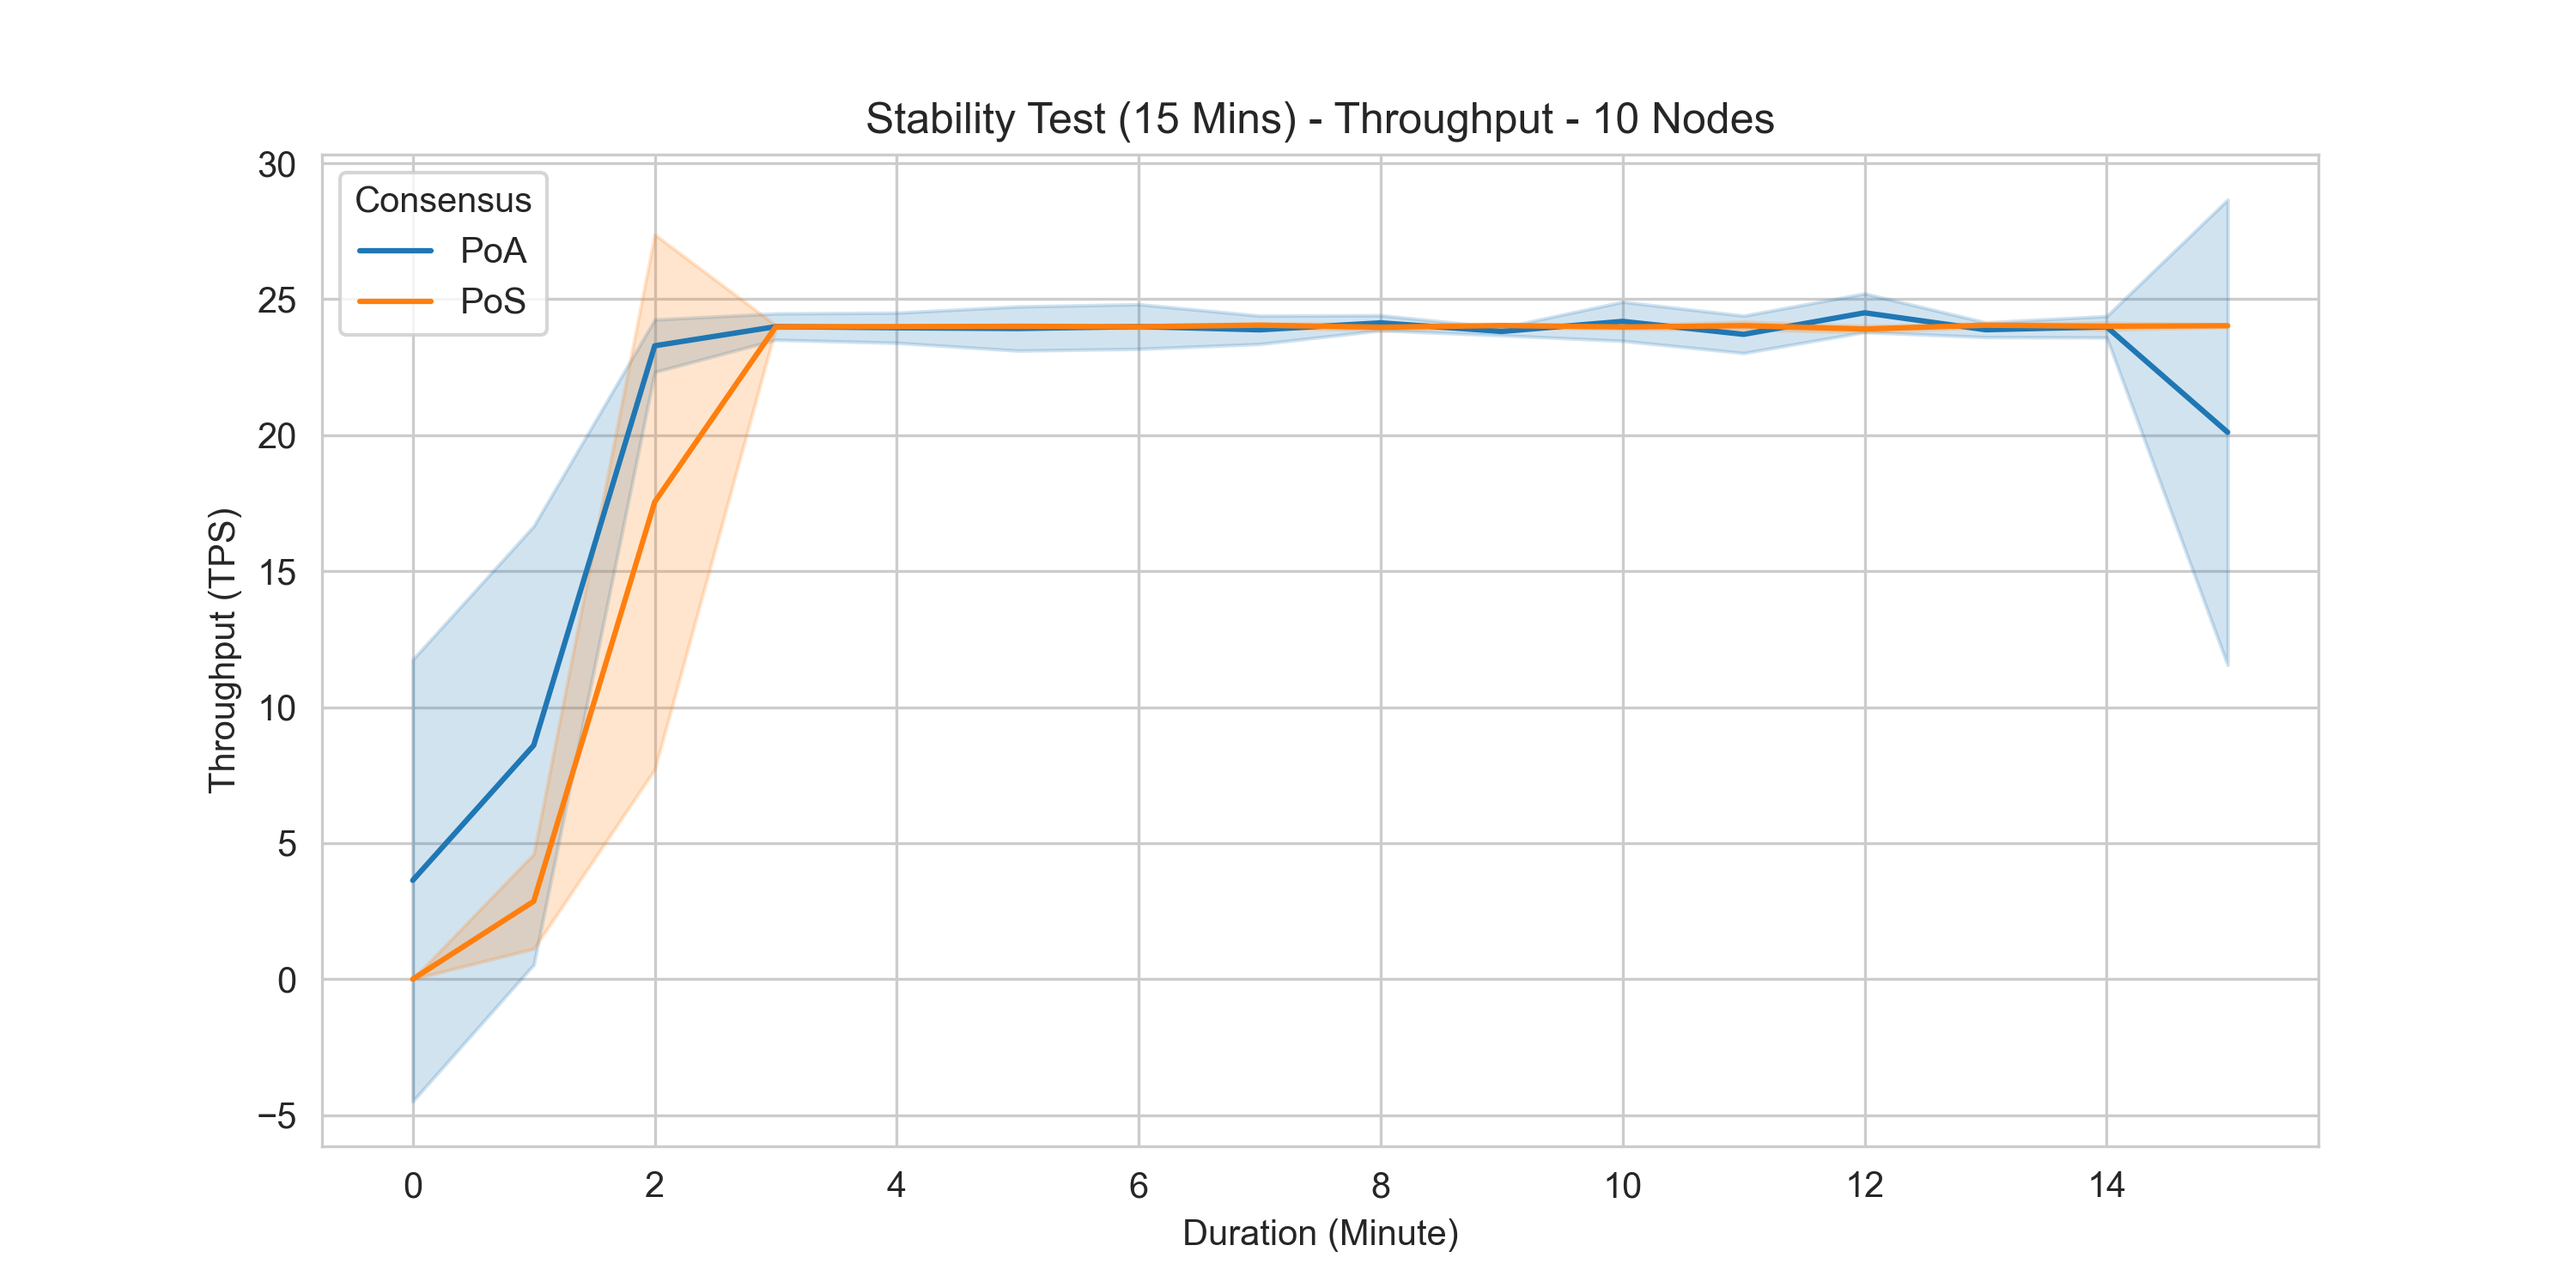
\includegraphics[width=0.9\textwidth]{images/stability_timeseries_tps_10_Nodes.png}
    \caption{Time Series TPS pada Uji Stabilitas (10 Node)}
    \label{fig:stability_timeseries_tps_10}
\end{figure}

\begin{figure}[htbp]
    \centering
    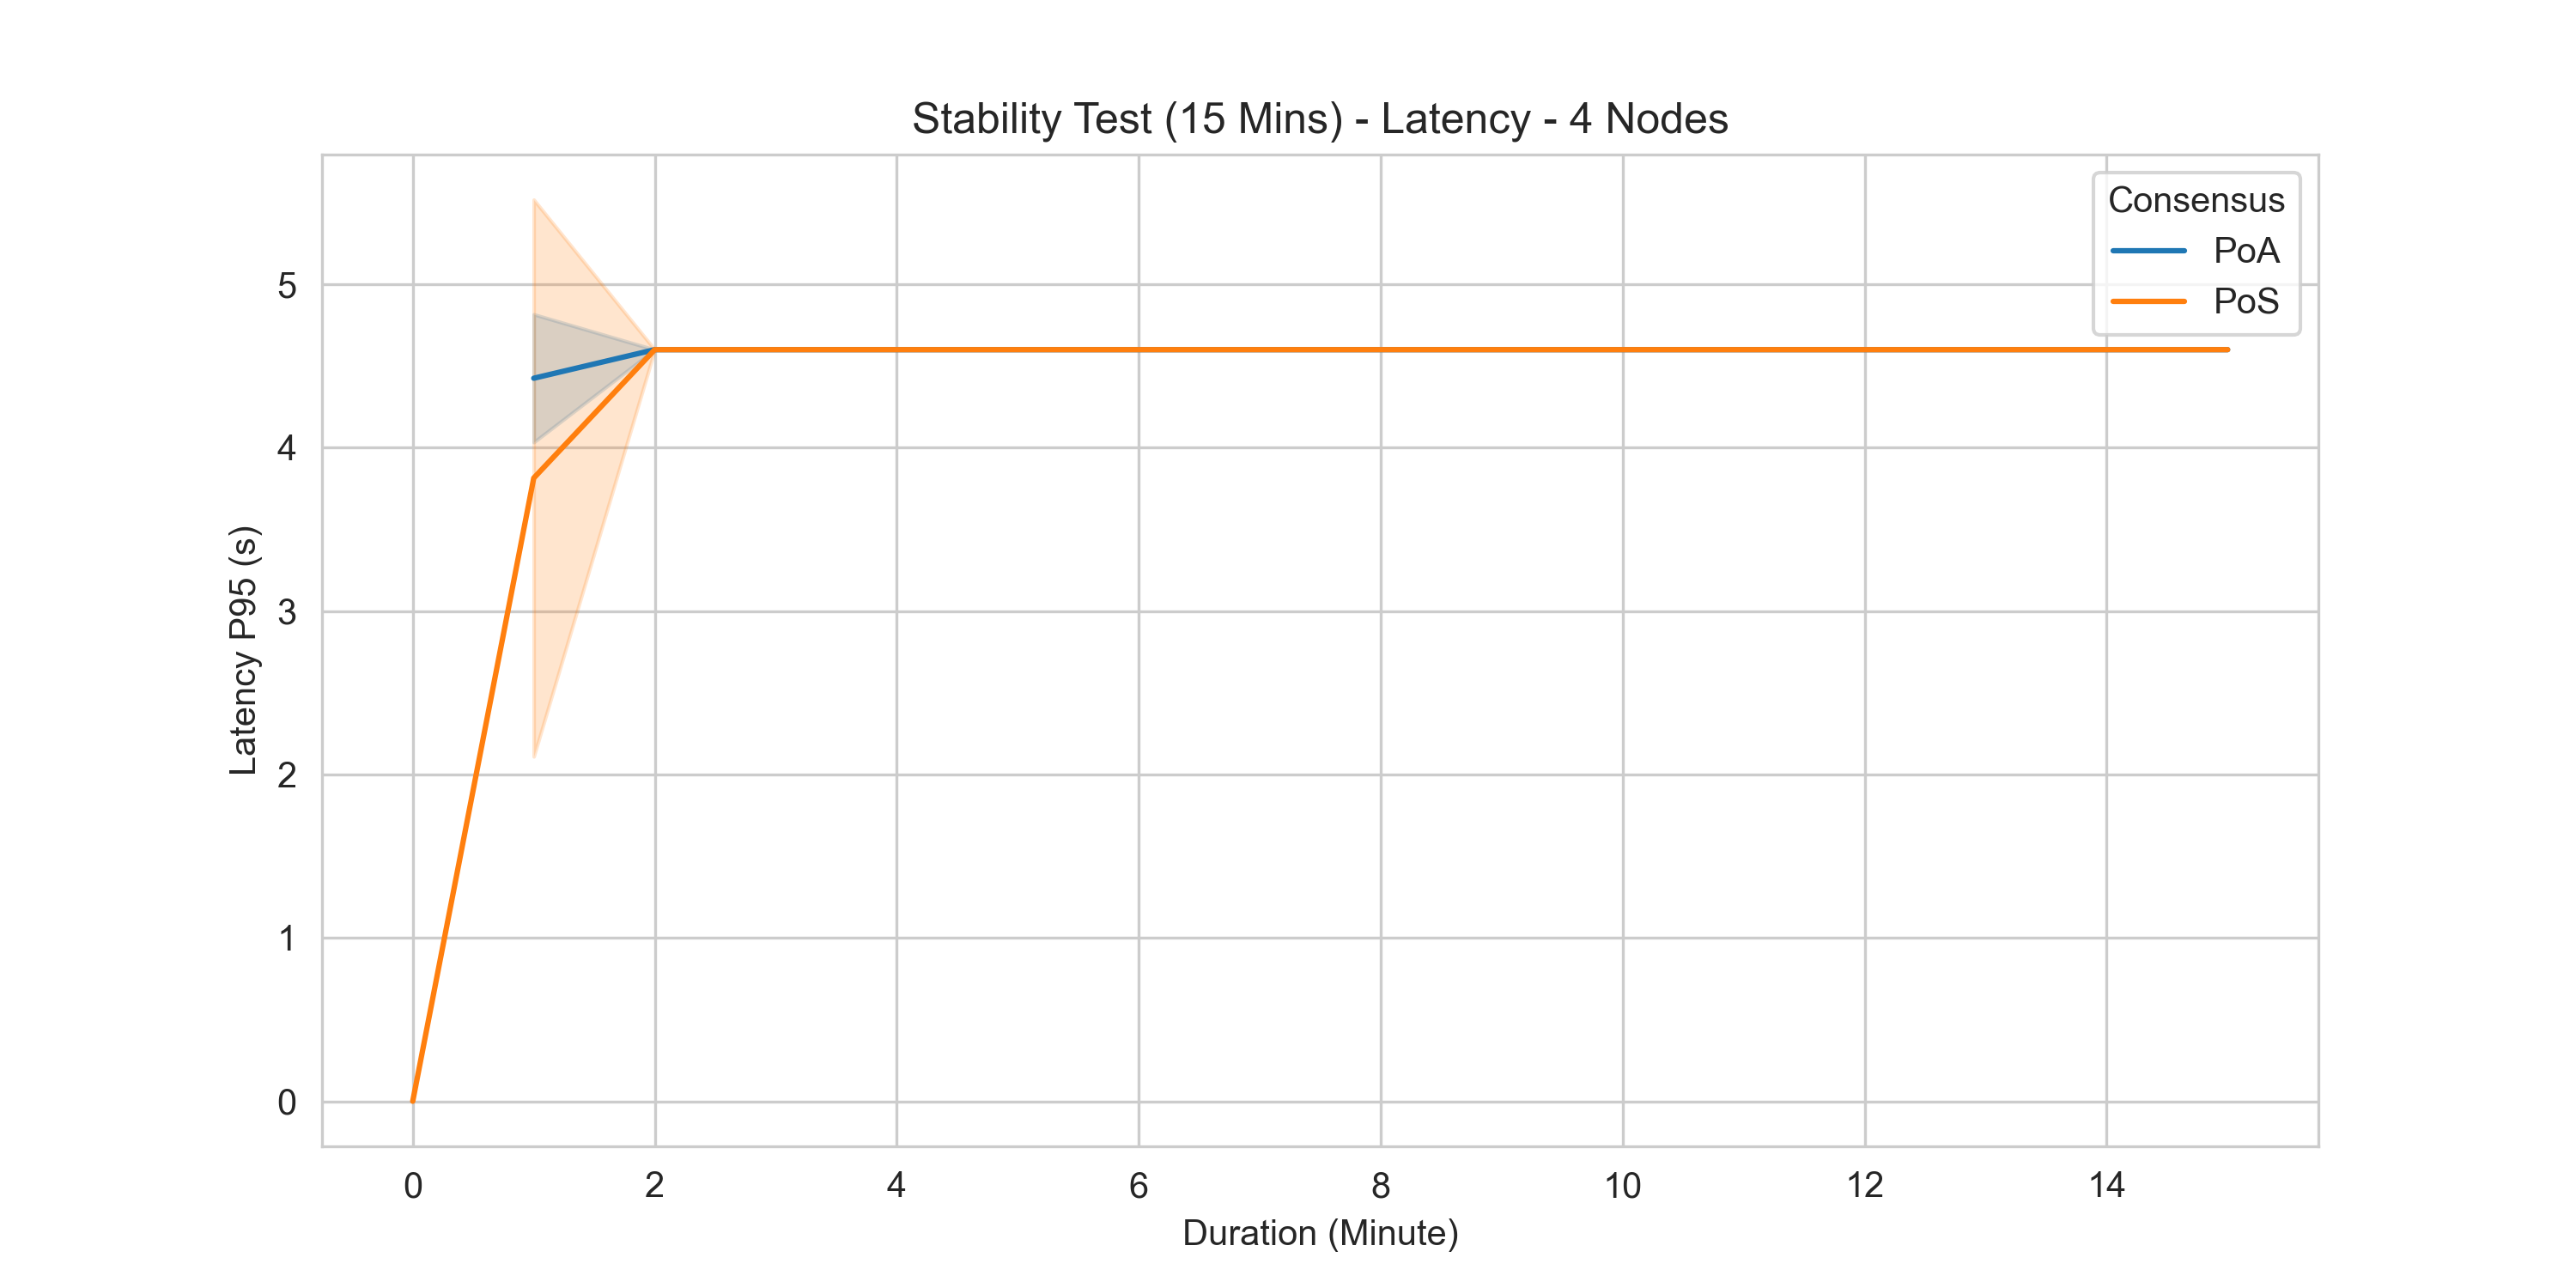
\includegraphics[width=0.9\textwidth]{images/stability_timeseries_latency_4_Nodes.png}
    \caption{Time Series Latency pada Uji Stabilitas (4 Node)}
    \label{fig:stability_timeseries_latency_4}
\end{figure}

\begin{figure}[htbp]
    \centering
    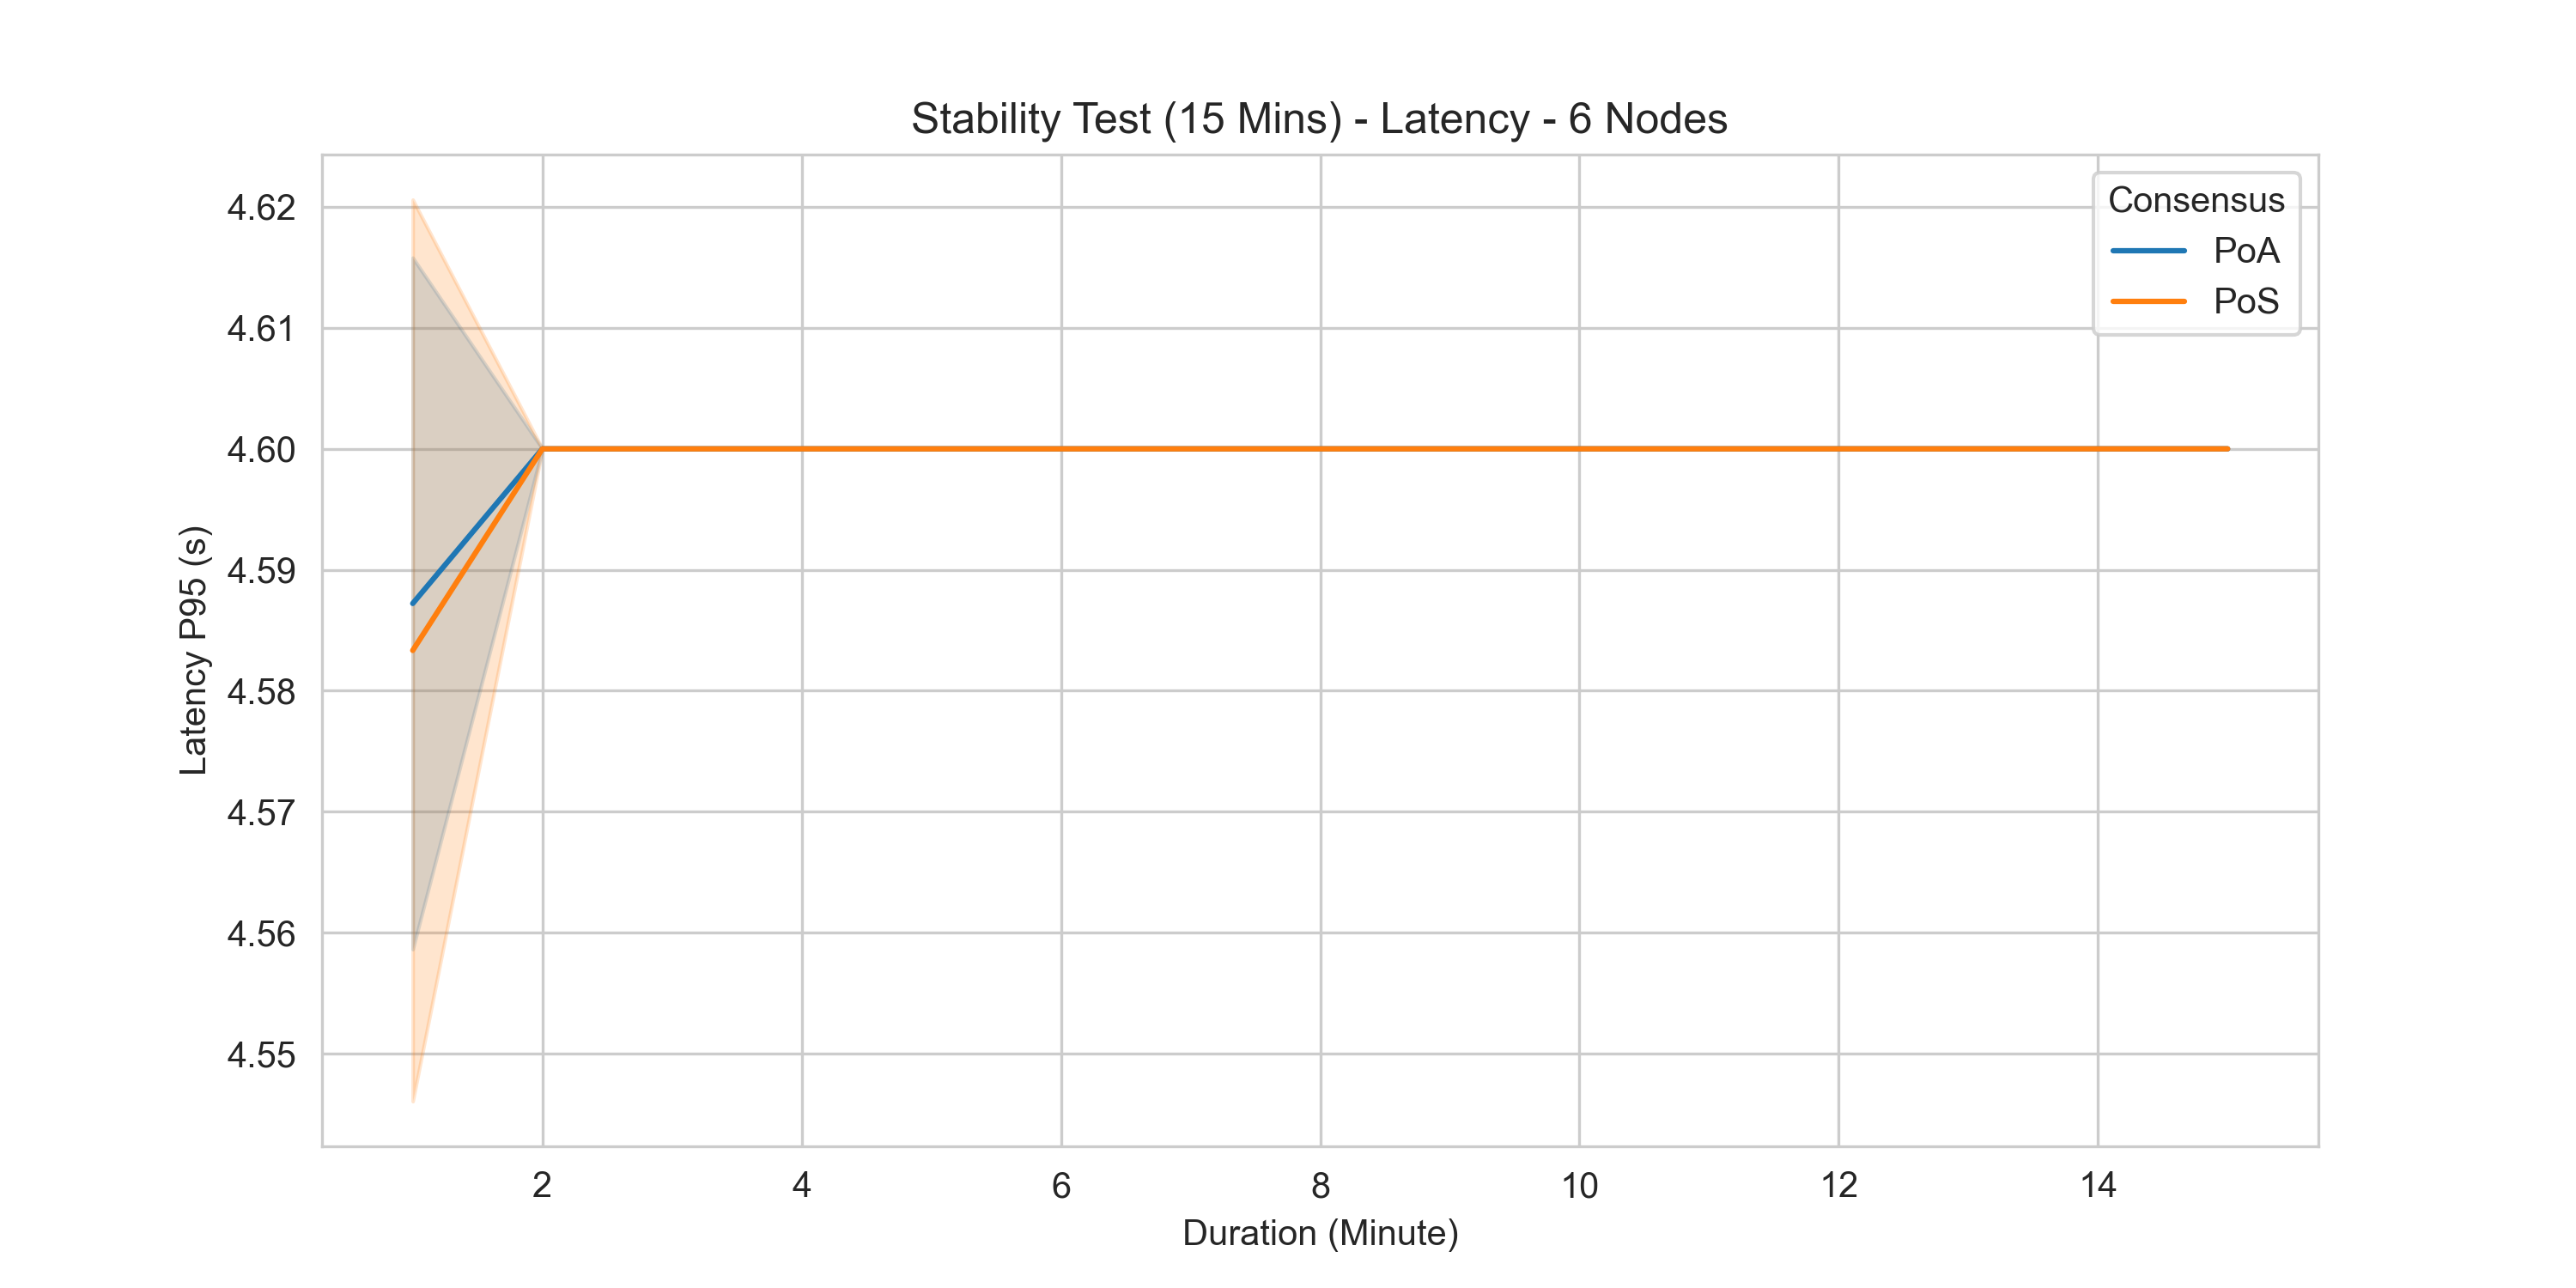
\includegraphics[width=0.9\textwidth]{images/stability_timeseries_latency_6_Nodes.png}
    \caption{Time Series Latency pada Uji Stabilitas (6 Node)}
    \label{fig:stability_timeseries_latency_6}
\end{figure}

\begin{figure}[htbp]
    \centering
    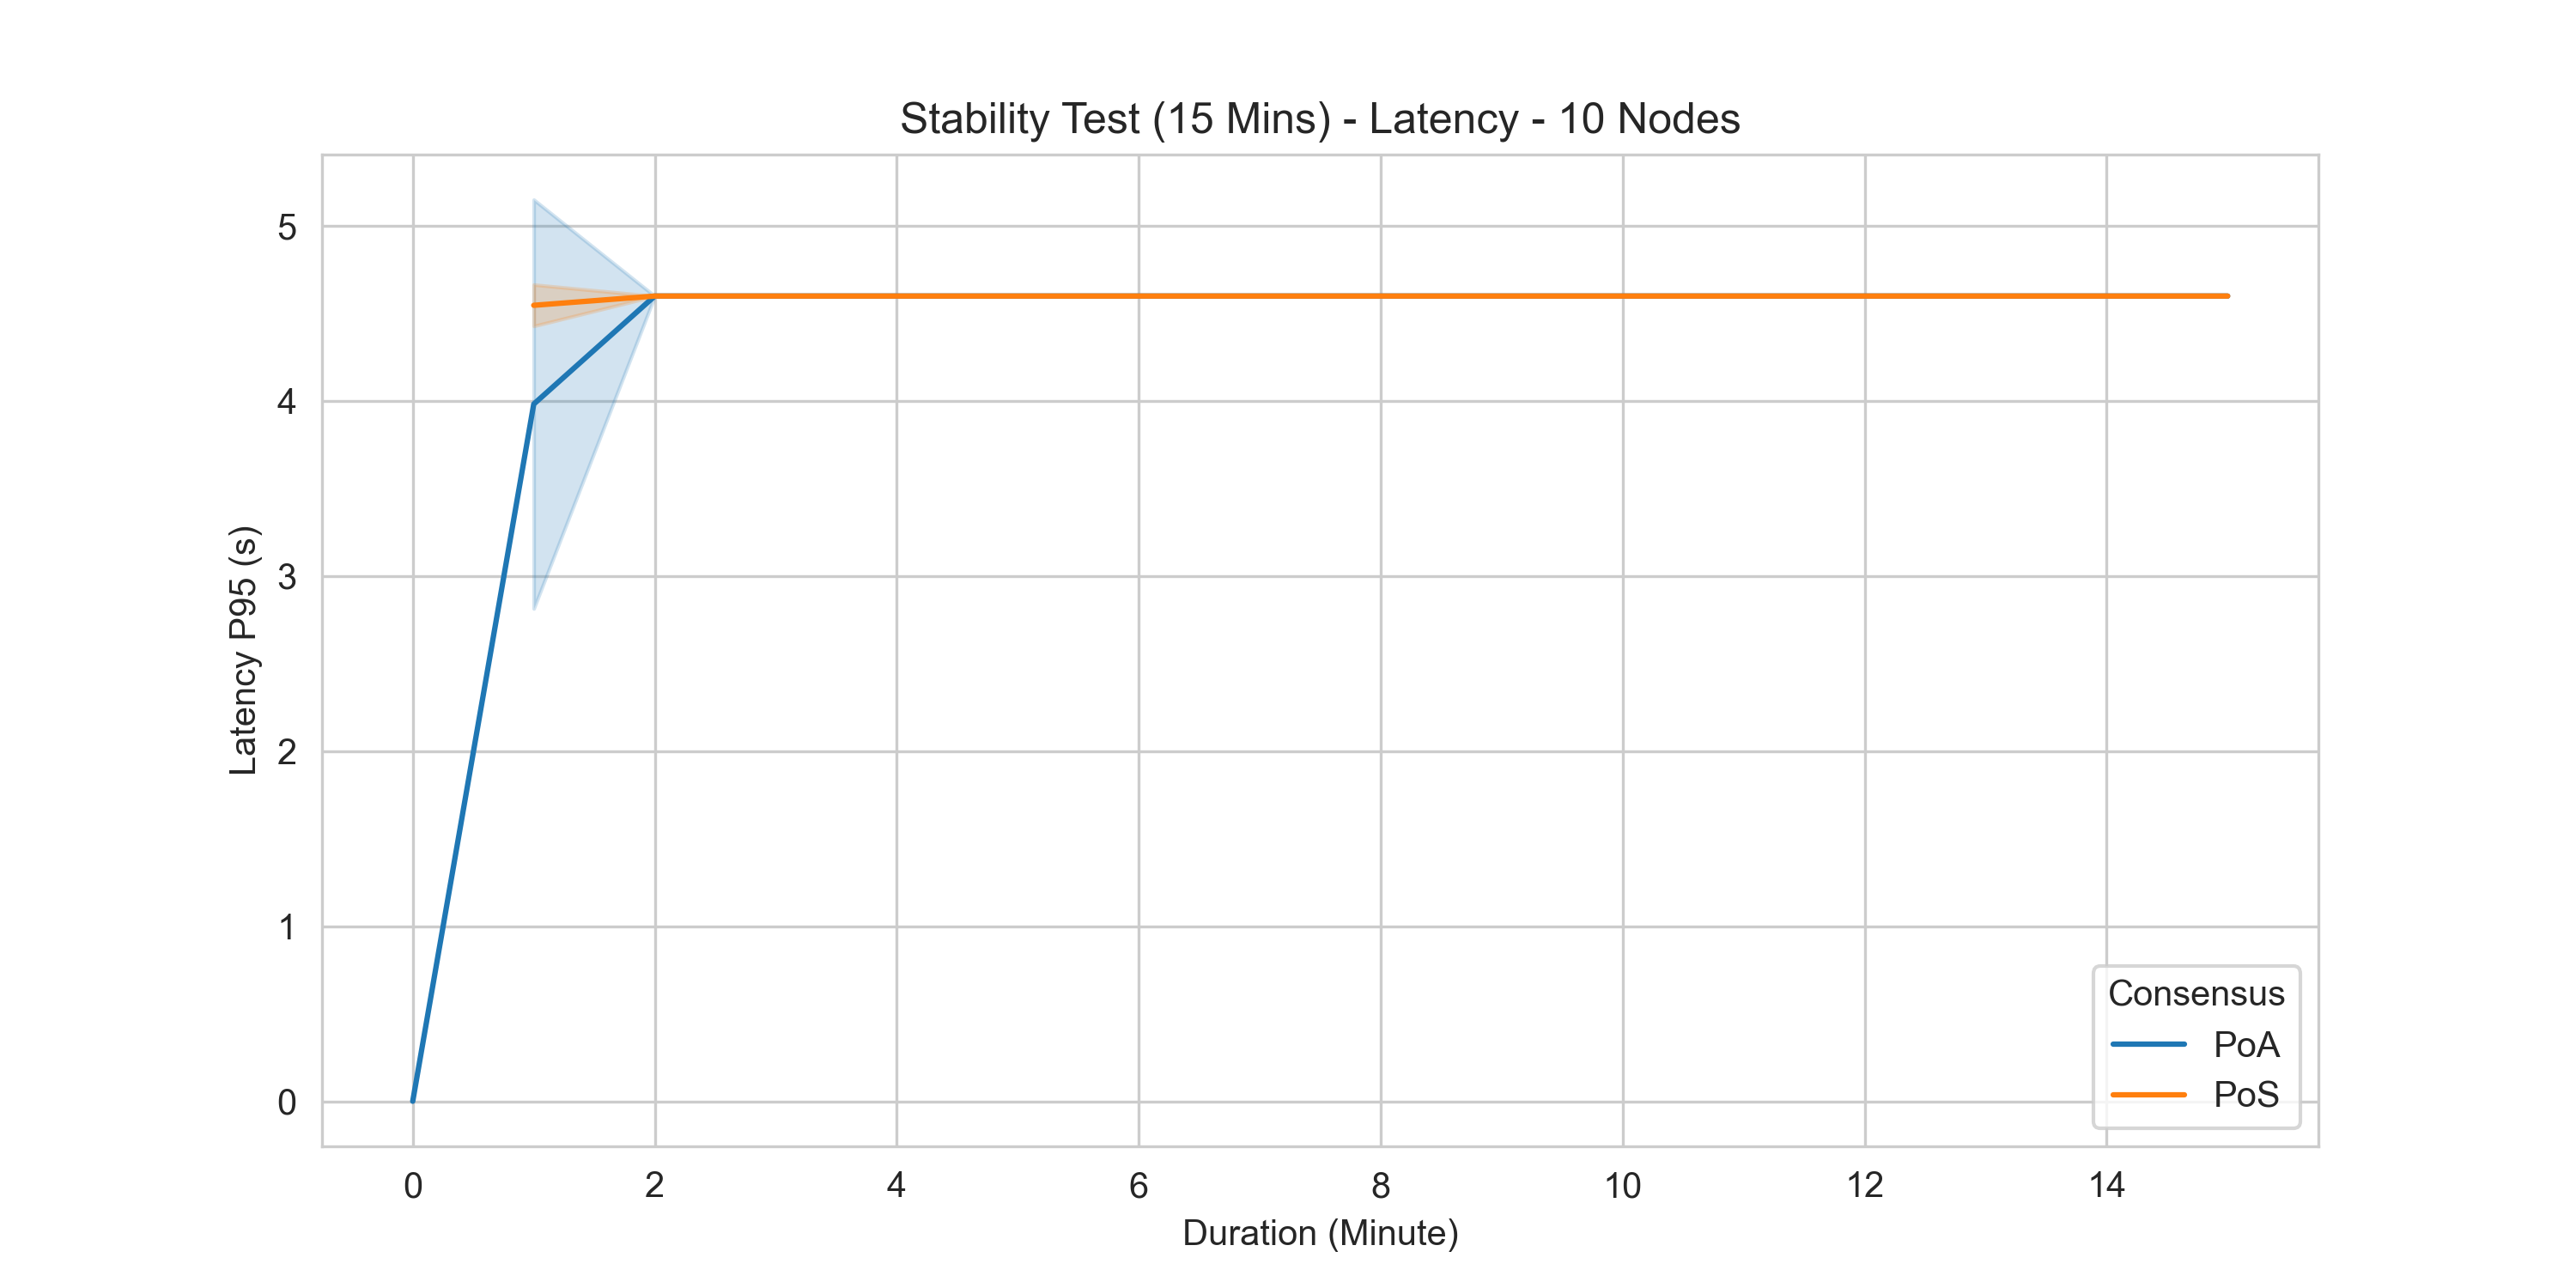
\includegraphics[width=0.9\textwidth]{images/stability_timeseries_latency_10_Nodes.png}
    \caption{Time Series Latency pada Uji Stabilitas (10 Node)}
    \label{fig:stability_timeseries_latency_10}
\end{figure}

\begin{figure}[htbp]
    \centering
    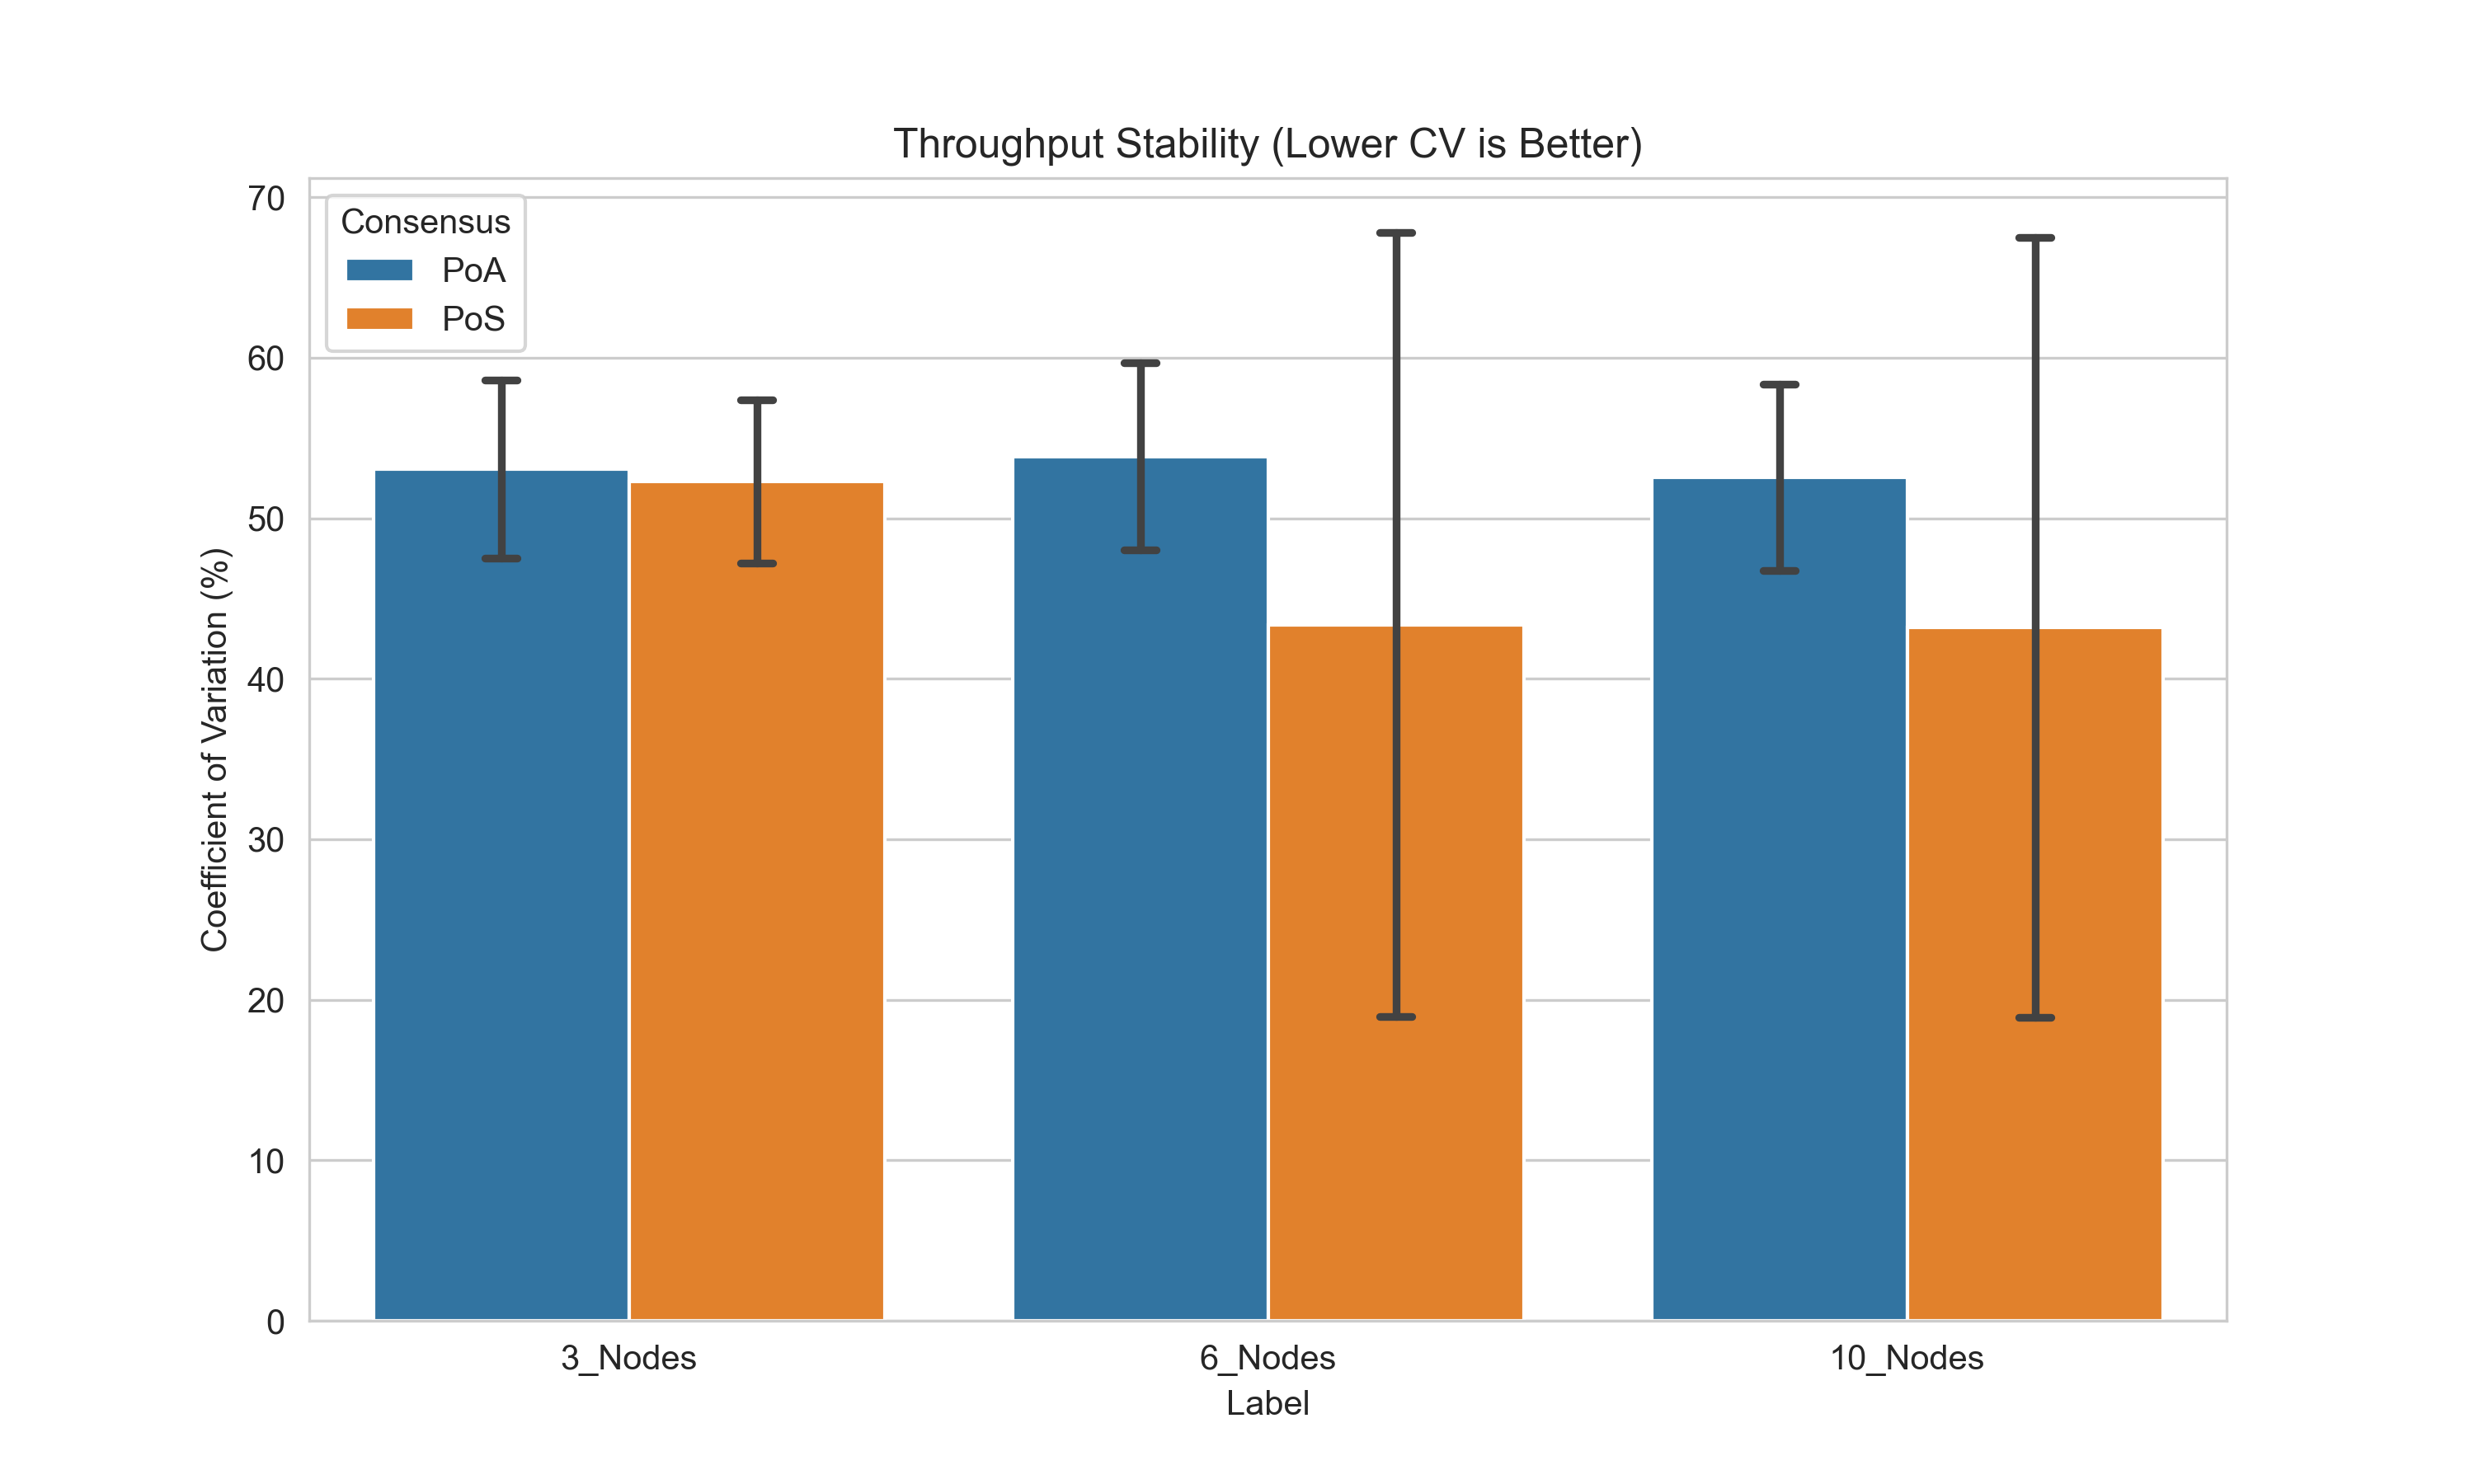
\includegraphics[width=0.9\textwidth]{images/stability_cv_comparison.png}
    \caption{Perbandingan Coefficient of Variation (Stabilitas)}
    \label{fig:stability_cv}
\end{figure}

\subsection{Skenario Fungsional (Lifecycle)}

Perbandingan latensi untuk tiga operasi utama: \textit{Mint}, \textit{Read}, dan \textit{Burn} ditampilkan pada Gambar \ref{fig:lifecycle_latency} dan Gambar \ref{fig:lifecycle_tps}.
\begin{itemize}
    \item \textbf{Mint (Write)}: PoA ($\approx 4.6$s) lebih cepat dibanding PoS ($\approx 8$s).
    \item \textbf{Read}: Keduanya instan ($\approx 0.01$s).
    \item \textbf{Burn}: Performanya identik dengan operasi \textit{Mint}.
\end{itemize}

\begin{figure}[htbp]
    \centering
    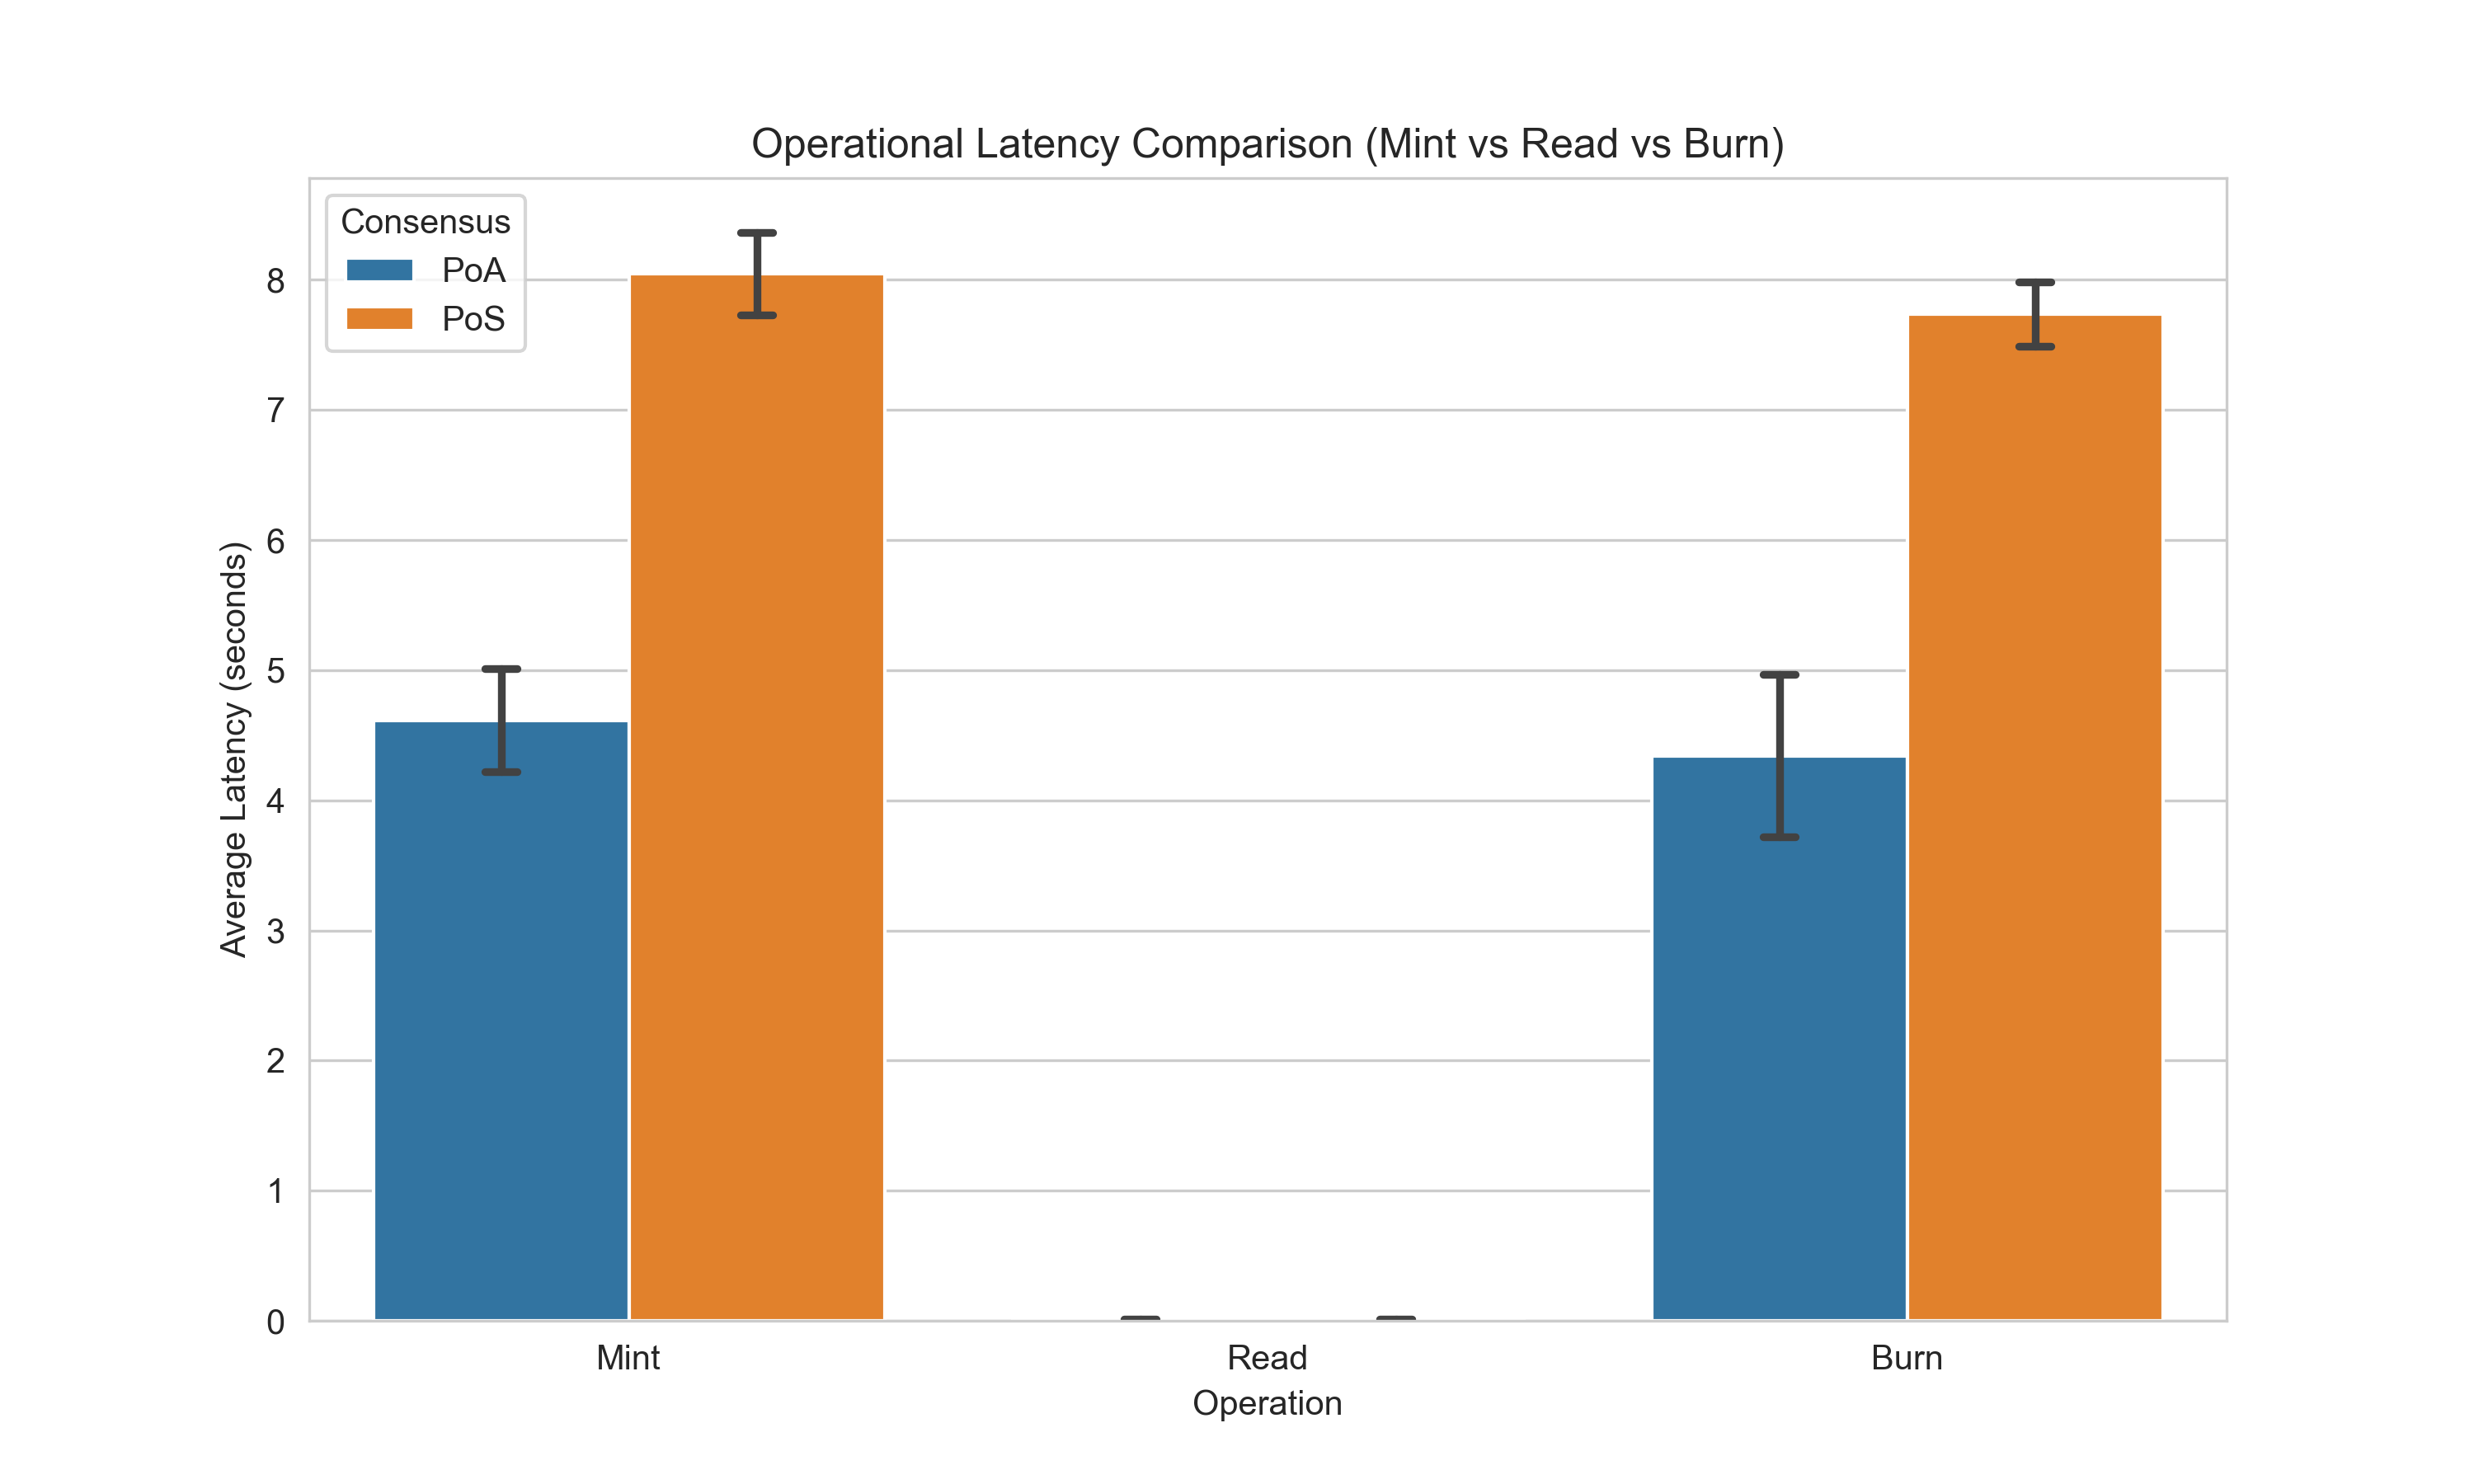
\includegraphics[width=0.9\textwidth]{images/lifecycle_latency_comparison.png}
    \caption{Perbandingan Latensi Operasi Lifecycle}
    \label{fig:lifecycle_latency}
\end{figure}

\begin{figure}[htbp]
    \centering
    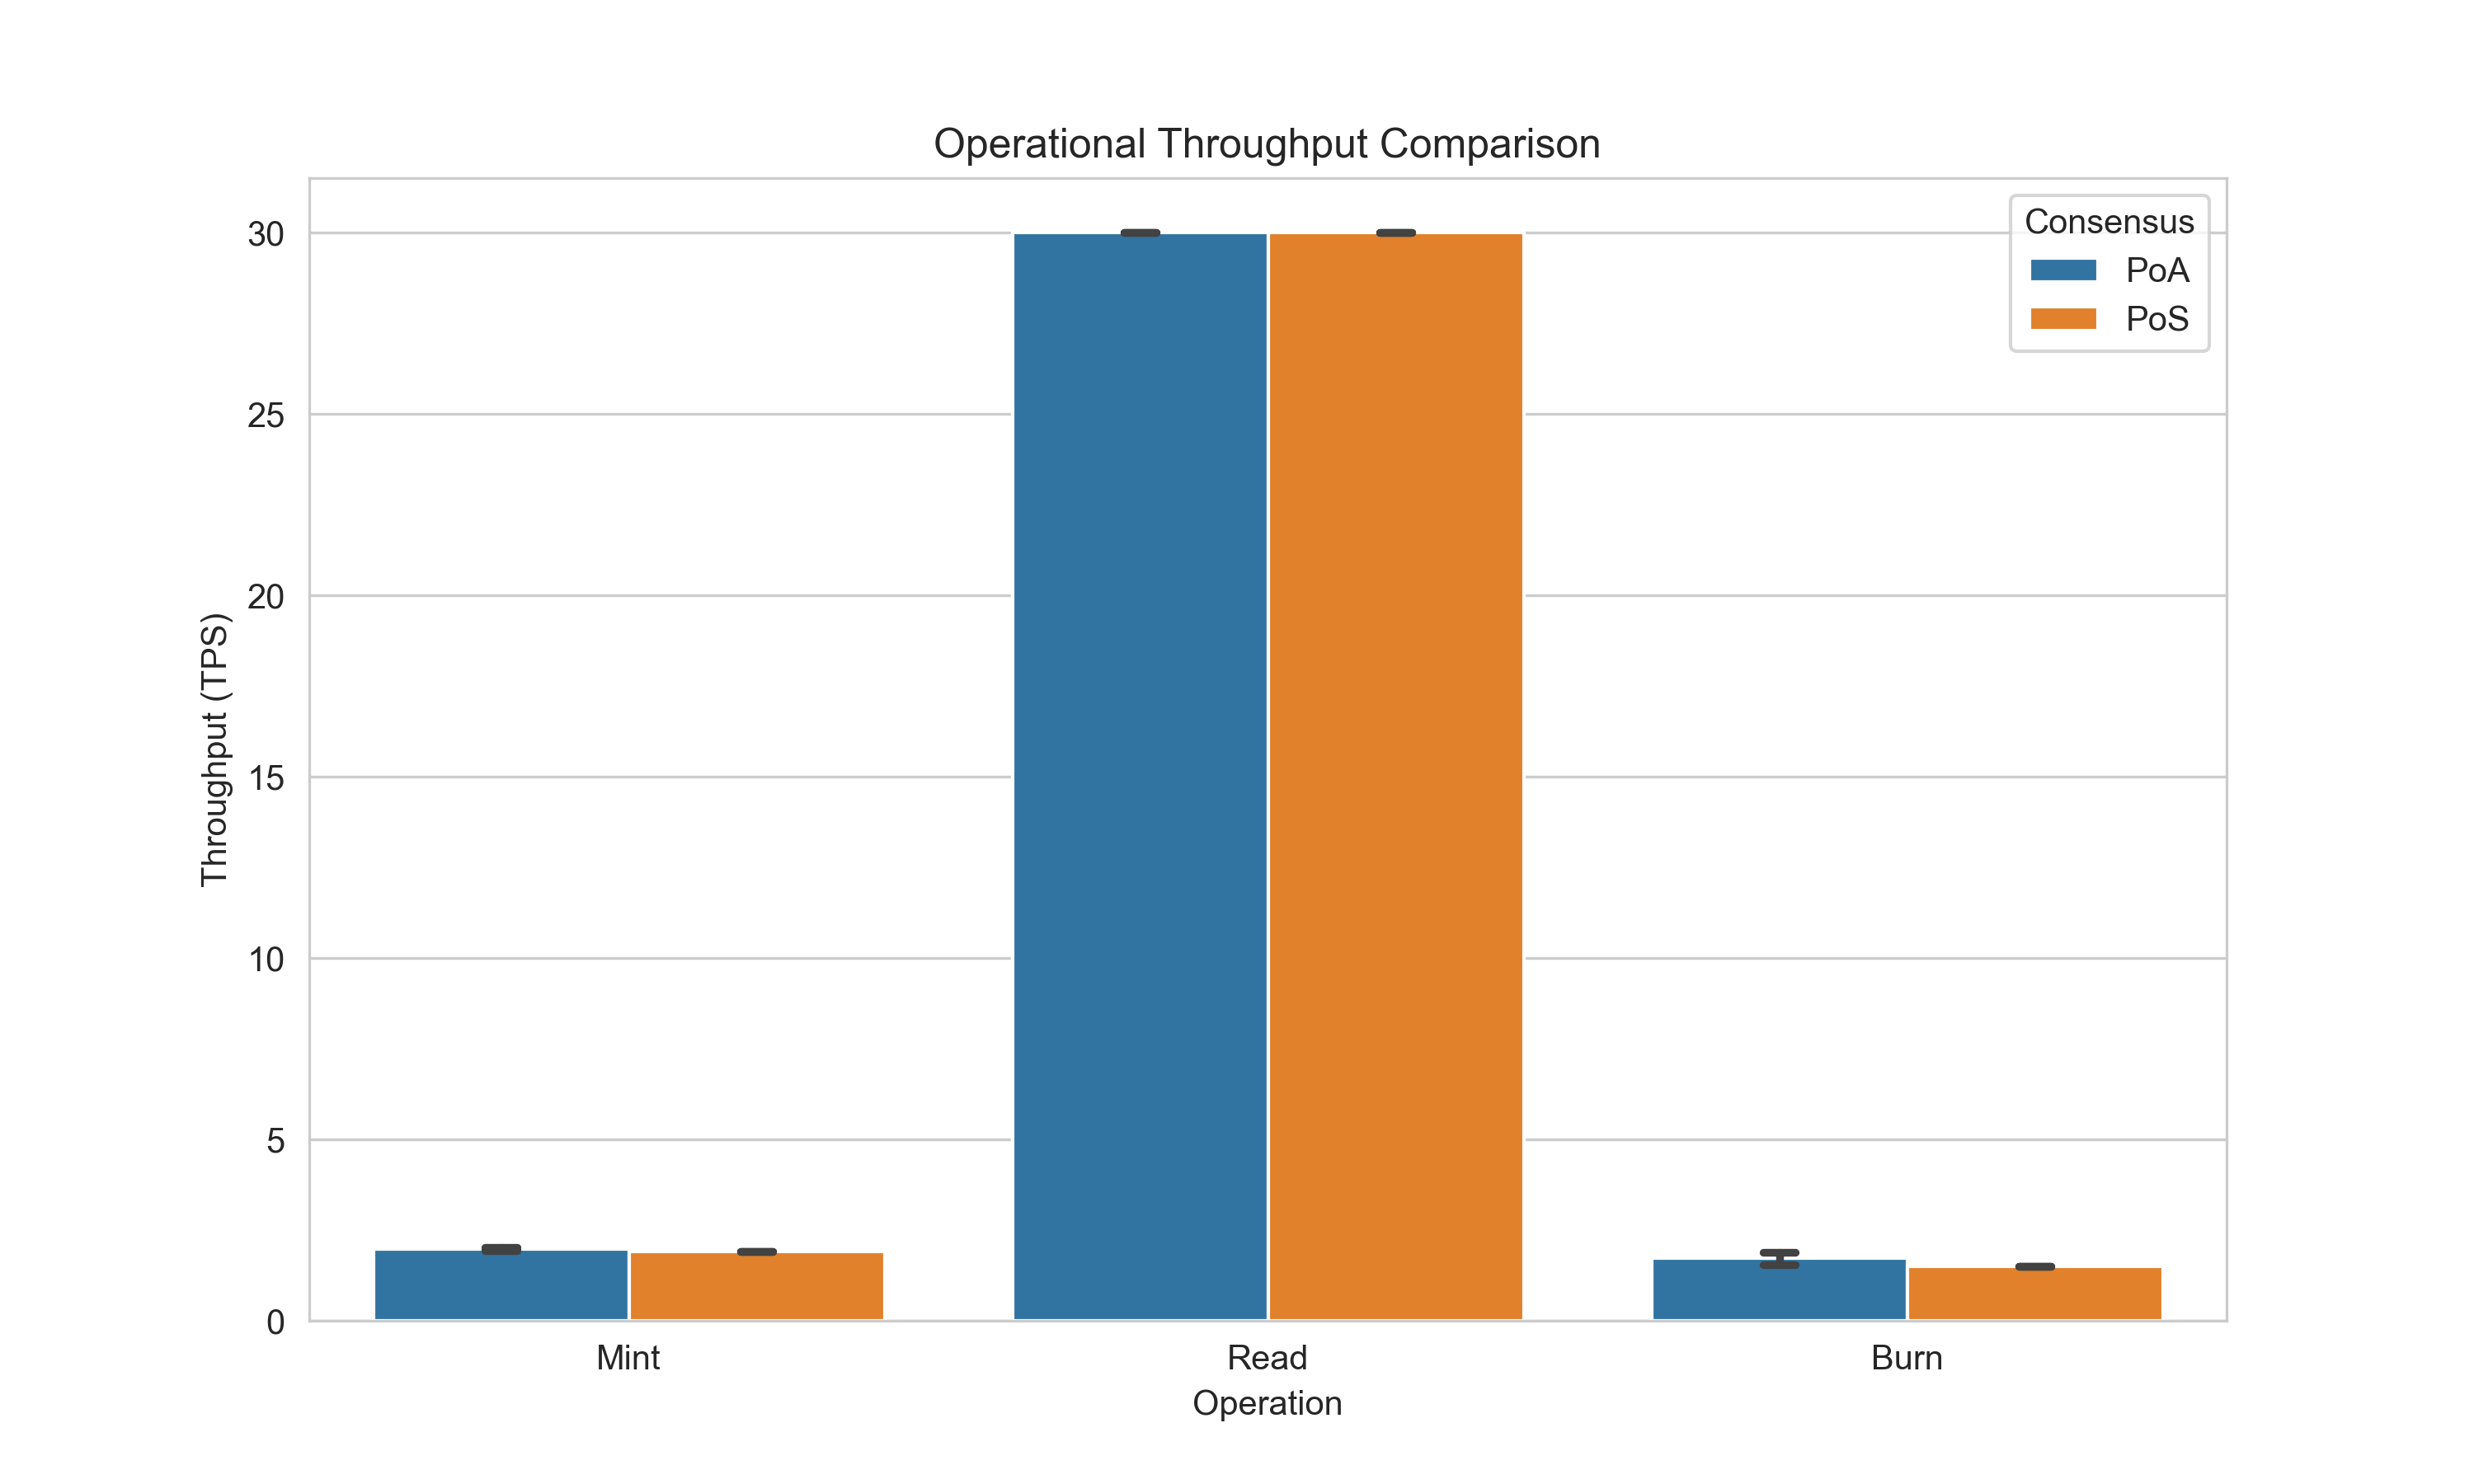
\includegraphics[width=0.9\textwidth]{images/lifecycle_tps_comparison.png}
    \caption{Perbandingan TPS Operasi Lifecycle}
    \label{fig:lifecycle_tps}
\end{figure}

\section{Analisis dan Pembahasan}

\subsection{Analisis Performa Throughput dan Skalabilitas}

Data menunjukkan fenomena menarik di mana PoS justru mencapai \textit{throughput} saturasi 2x lebih tinggi dibanding PoA pada skala kecil (4 Node). Hal ini diduga disebabkan oleh batasan \textit{Block Time}. PoA dengan blok 5 detik memiliki batas fisik jumlah gas/blok per satuan waktu. Sebaliknya, PoS dengan slot 12 detik, meskipun intervalnya lebih lama, memungkinkan \textit{batching} transaksi yang lebih efisien dengan batas gas yang sama per blok, menghasilkan \textit{throughput} agregat yang lebih tinggi sebelum saturasi RPC.

Namun, skalabilitas klien menunjukkan pola \textit{Sub-linear} untuk kedua konsensus, mengindikasikan bahwa \textit{bottleneck} utama bukan pada lapisan konsensus, melainkan pada lapisan RPC Node atau antrian transaksi di Caliper.

\subsection{Analisis Responsivitas dan Latensi}

PoA menunjukkan keunggulan telak dalam aspek responsivitas. Rata-rata latensi PoA (4.6 detik) sangat mendekati waktu blok (5 detik), menunjukkan inefisiensi minimal. Sebaliknya, PoS (8 detik) menderita latensi inheren dari mekanisme slot dan finalitas probabilistik awal. Untuk sistem layanan akademik, perbedaan 3--4 detik ini signifikan secara UX (\textit{User Experience}).

\subsection{Analisis Efisiensi dan Stabilitas}

PoA unggul dalam efisiensi sumber daya. PoS "membayar" desentralisasinya dengan komputasi mahal untuk \textit{attestation}. Stabilitas kedua sistem terbukti tangguh dalam uji jangka panjang (\textit{Soak Test}), tidak ditemukan indikasi kebocoran memori.

\subsection{Sintesis Visual: Trade-off Multidimensi}

Gambar \ref{fig:radar_chart} menyajikan sintesis karakteristik performa kedua konsensus dalam diagram radar lima dimensi. Setiap sumbu merepresentasikan skor 1-10 (semakin luar semakin baik).

Skor pada diagram ini merupakan hasil normalisasi kualitatif dari data kuantitatif yang diperoleh pada pengujian sebelumnya. Skala 1-10 digunakan untuk memvisualisasikan performa relatif, di mana nilai 10 merepresentasikan capaian terbaik dalam eksperimen ini. Sebagai contoh, pada dimensi \textit{Throughput}, PoS diberi skor 10 karena mencapai saturasi tertinggi ($\approx$60 TPS), sedangkan PoA diberi skor 5 karena hanya mencapai setengahnya ($\approx$30 TPS). Metode ini diterapkan secara konsisten pada dimensi lain untuk memudahkan pembandingan trade-off secara visual.

Interpretasi dari grafik tersebut adalah:
\begin{itemize}
    \item \textbf{Throughput (Capacity)}: PoS unggul signifikan (Skor 10), mencapai volume transaksi tertinggi.
    \item \textbf{Responsiveness}: PoA unggul (Skor 9) dengan latensi yang lebih rendah dan waktu blok lebih singkat.
    \item \textbf{Resource Efficiency}: PoA sangat dominan (Skor 9), sangat hemat CPU.
    \item \textbf{Stability}: Keduanya seimbang, namun PoA sedikit lebih stabil (CV Score lebih baik).
    \item \textbf{Finality Speed}: PoA Clique memberikan finalitas yang lebih cepat untuk aplikasi pengguna karena sifat deterministiknya.
\end{itemize}

Secara keseluruhan, PoA membentuk area grafik yang condong ke sisi efisiensi dan responsivitas, sedangkan PoS condong ke sisi kapasitas murni.

\begin{figure}[htbp]
    \centering
    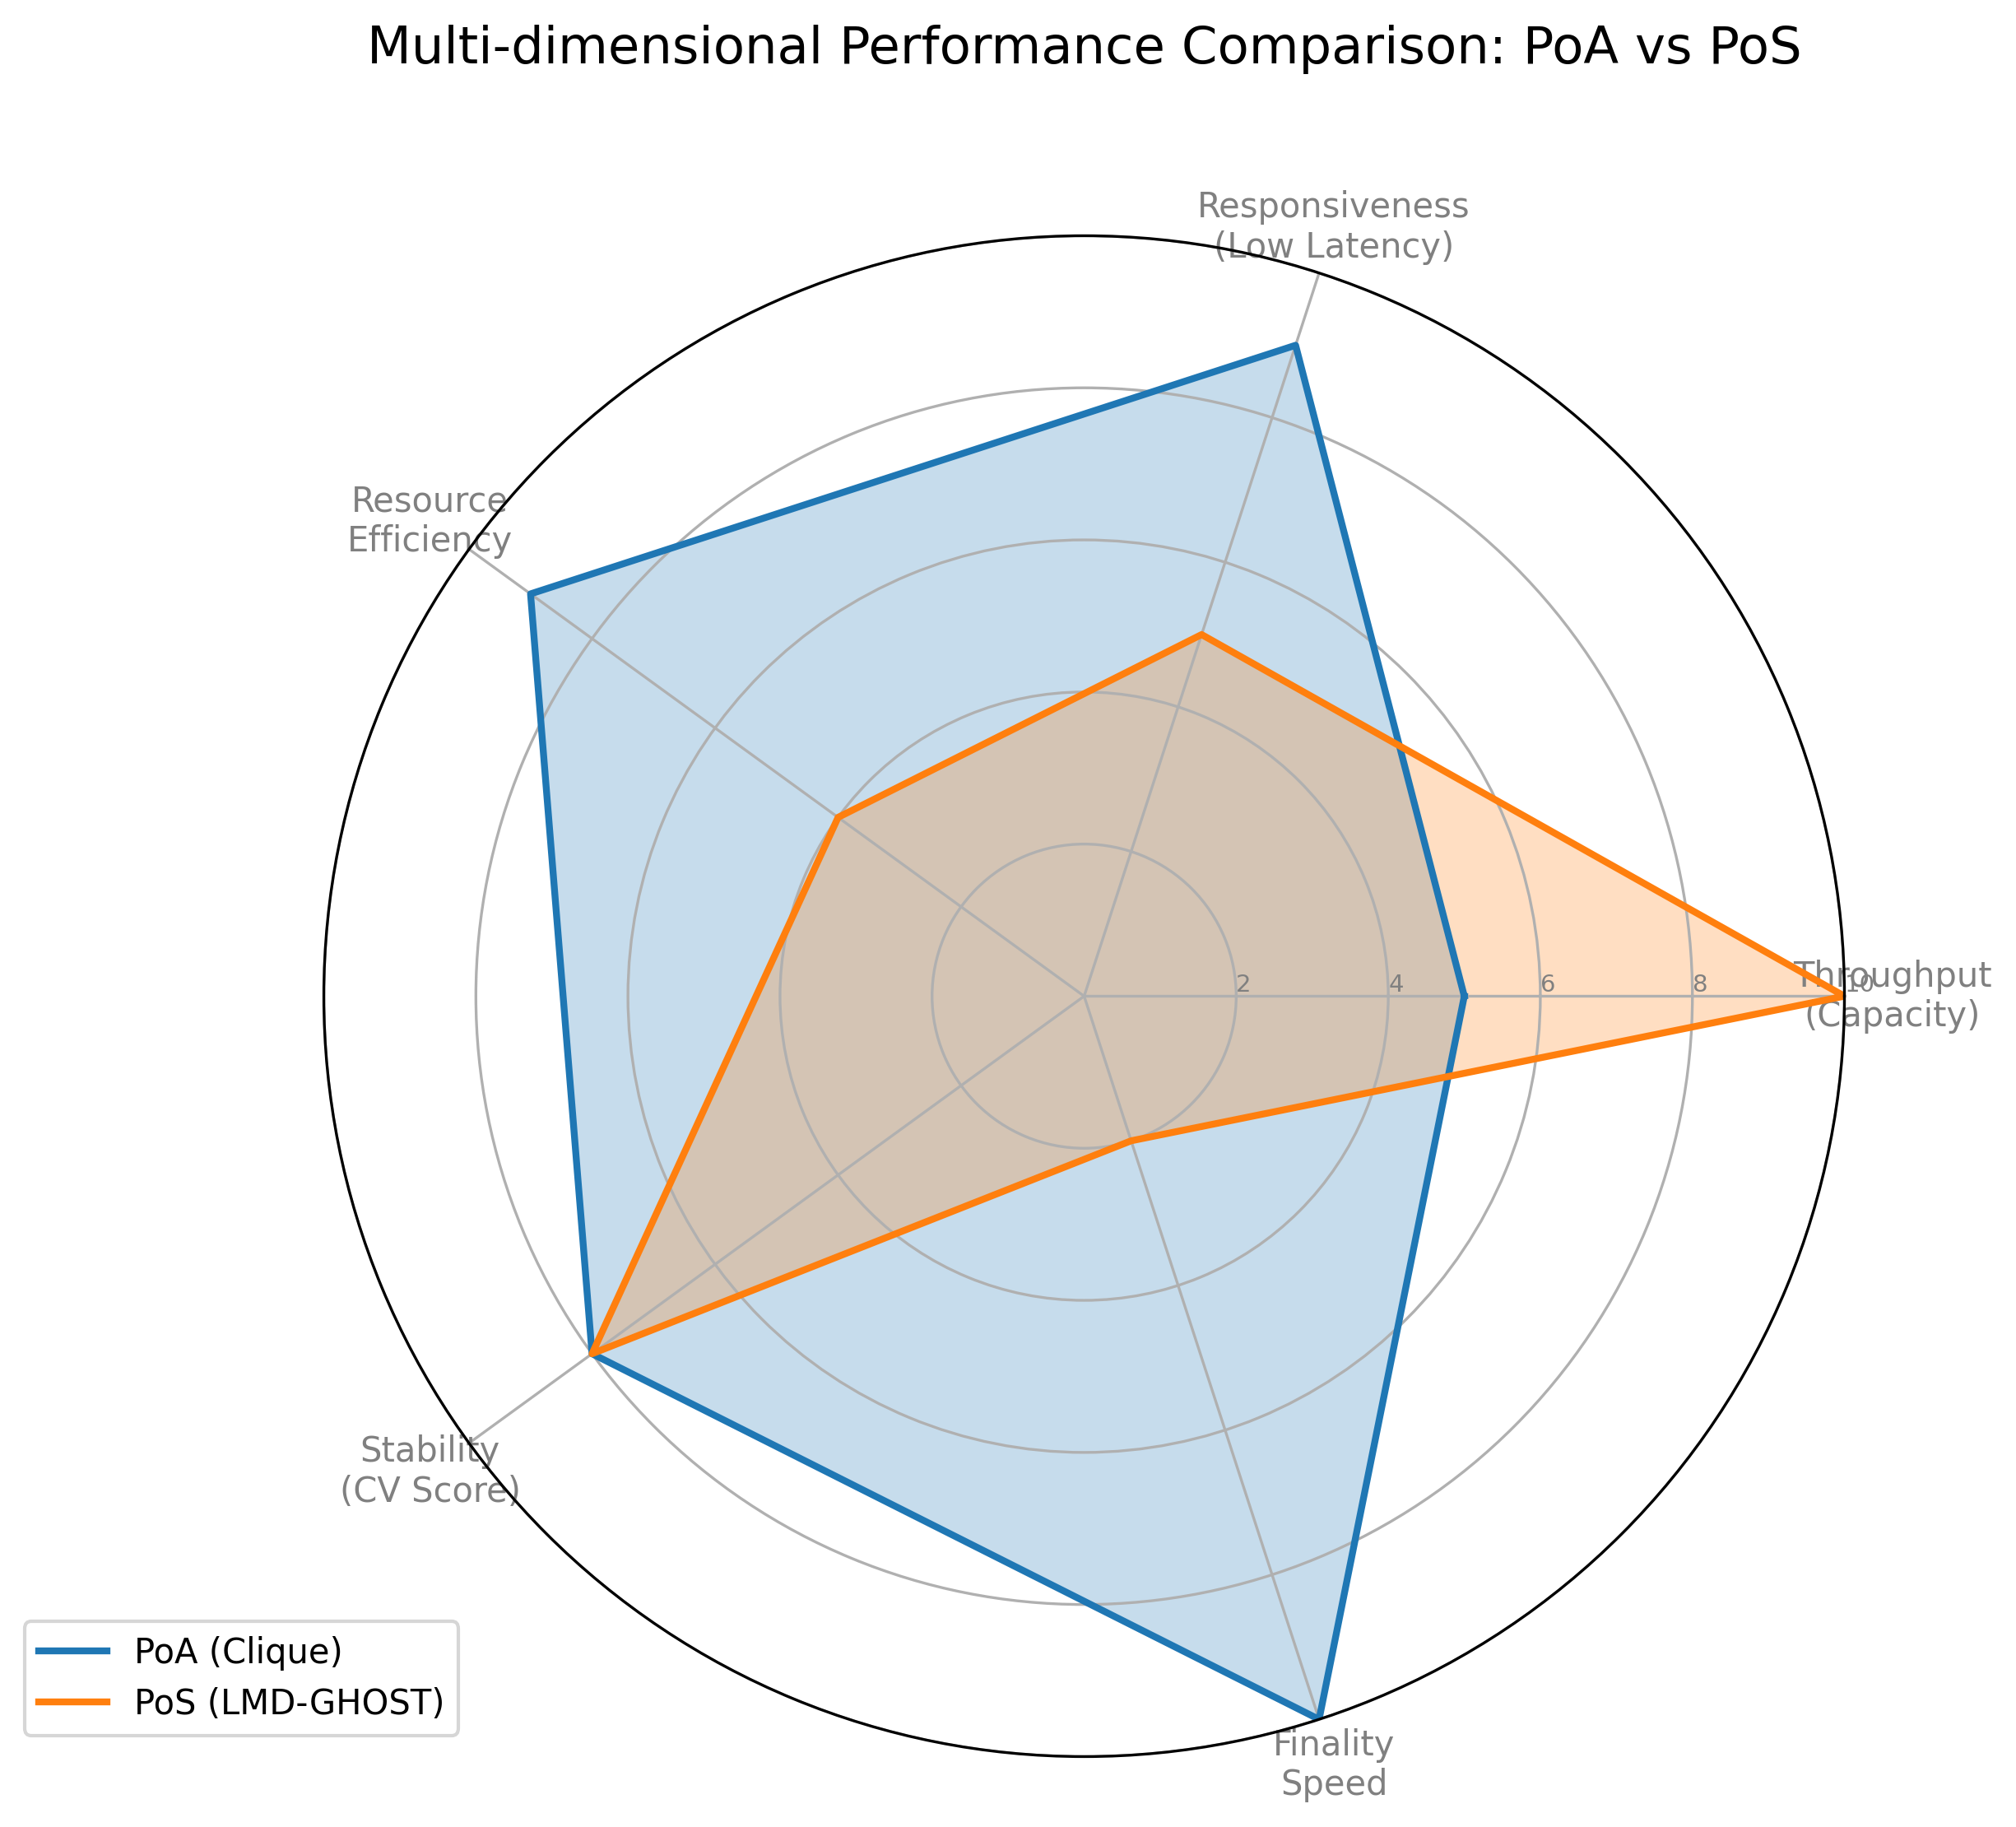
\includegraphics[width=0.8\textwidth]{images/radar_chart_comparison.png}
    \caption{Radar Chart Perbandingan PoA vs PoS}
    \label{fig:radar_chart}
\end{figure}

\subsection{Sintesis Akhir: Relevansi untuk DChain}
Untuk kasus penggunaan sertifikat akademik di DChain, karakteristik \textbf{PoA} terbukti lebih menguntungkan karena:
\begin{enumerate}
    \item \textbf{User-Interactive}: Latensi rendah memberikan pengalaman pengguna yang lebih baik.
    \item \textbf{Read-Heavy}: Volume transaksi tulis (penerbitan ijazah) relatif rendah dan musiman, sehingga kapasitas masif PoS kurang termanfaatkan dibanding efisiensi biaya operasional PoA.
    \item \textbf{Finalitas}: PoA Clique menawarkan finalitas deterministik yang lebih sederhana untuk integrasi aplikasi.
\end{enumerate}

\section{Perbandingan dengan Penelitian Terdahulu}

Penelitian ini memberikan kontribusi empiris dengan membandingkan hasil pengujian DChain terhadap literatur yang ada, sebagaimana dirangkum dalam Tabel \ref{tab:comparison_literature}.

\begin{table}[htbp]
\centering
\caption{Perbandingan Hasil DChain dengan Literatur Terdahulu}
\label{tab:comparison_literature}
\begin{tabularx}{\textwidth}{|>{\RaggedRight\arraybackslash}p{2.5cm}|>{\RaggedRight\arraybackslash}X|>{\RaggedRight\arraybackslash}X|>{\RaggedRight\arraybackslash}p{4cm}|}
\hline
\textbf{Aspek} & \textbf{Temuan DChain} & \textbf{Penelitian Terdahulu} & \textbf{Analisis} \\
\hline
\textbf{Throughput} & $\approx$30--40 TPS (Saturasi Awal) & PoA $>1000$ TPS \cite{choi2020,rebello2020} & Hasil DChain lebih rendah karena menggunakan VPS \textit{resource} terbatas dan latensi geografis nyata, mencerminkan kondisi riil. \\
\hline
\textbf{Latensi} & $\approx$4--5 detik & PoA $<1$ detik \cite{arslan2020,wicaksono2025} & Konsisten dengan konfigurasi \textit{block time} 5 detik. Penelitian Wicaksono \cite{wicaksono2025} juga menemukan latensi serupa pada \textit{load} moderat. \\
\hline
\textbf{Efisiensi} & Sangat Tinggi (TPS/\%CPU) & Dianggap efisien \cite{sharma2020,ali2020} & Validasi temuan bahwa PoA jauh lebih ringan dibanding PoS. \\
\hline
\end{tabularx}
\end{table}

Berdasarkan analisis pada Tabel \ref{tab:comparison_literature}, penelitian ini mengisi celah (\textit{research gap}) dengan:
\begin{enumerate}
    \item \textbf{Studi Kasus Spesifik}: Menguji beban kerja fungsional (\textit{Lifecycle}) yang relevan secara bisnis, bukan sekadar transfer token.
    \item \textbf{Topologi Geografis Nyata}: Simulasi latensi antar-kampus (UGM, UI, ITB), bukan \textit{localhost}.
    \item \textbf{Analisis Stabilitas}: Menambahkan uji \textit{Soak Test} untuk membuktikan ketahanan sistem.
\end{enumerate}
\cleardoublepage \phantomsection
\chapter{Kesimpulan dan Saran}

\section{Kesimpulan}

Penelitian ini bertujuan untuk mengevaluasi dan membandingkan kinerja mekanisme konsensus \textit{Proof of Authority} (PoA) dan \textit{Proof of Stake} (PoS) dalam konteks implementasi infrastruktur sertifikat elektronik perguruan tinggi (DChain). Melalui serangkaian pengujian \textit{benchmarking} yang komprehensif menggunakan Hyperledger Caliper pada lingkungan \textit{multi-node} terdistribusi, penelitian ini telah berhasil menjawab rumusan masalah dan menguji hipotesis yang diajukan.

Berdasarkan analisis data empiris yang diperoleh dari 300+ iterasi uji coba, dapat ditarik beberapa kesimpulan utama sebagai berikut:

\begin{enumerate}
    \item \textbf{Trade-off Antara Kapasitas dan Responsivitas} \\
    Hasil penelitian menunjukkan adanya karakteristik kinerja yang bertolak belakang di antara kedua algoritma. \textbf{PoS unggul dalam aspek kapasitas} (\textit{throughput}) dengan capaian puncak hingga $\approx$60 TPS, hampir dua kali lipat lebih tinggi dibandingkan PoA yang mengalami saturasi pada $\approx$30--40 TPS. Namun, keunggulan ini harus dibayar dengan responsivitas yang lebih rendah. \textbf{PoA terbukti jauh lebih unggul dalam latensi}, mencatatkan waktu konfirmasi rata-rata 4.6 detik, yang secara signifikan lebih cepat dibandingkan PoS ($\approx$8 detik). Temuan ini memverifikasi bahwa PoA lebih cocok untuk aplikasi yang menuntut interaksi pengguna yang cepat (\textit{user-interactive}), sedangkan PoS lebih sesuai untuk pemrosesan data volume tinggi (\textit{batch processing}).

    \item \textbf{Efisiensi Sumber Daya} \\
    Dalam hal efisiensi operasional, \textbf{PoA menunjukkan superioritas} dalam pemanfaatan sumber daya komputasi. PoA mampu menghasilkan transaksi per detik per unit CPU (TPS/\%CPU) yang lebih tinggi dibandingkan PoS. Hal ini disebabkan oleh arsitektur PoS yang lebih kompleks, yang melibatkan dua lapisan proses (\textit{Execution Layer} dan \textit{Consensus Layer}) serta lalu lintas komunikasi \textit{gossip} antar-validator yang intensif, sehingga menciptakan \textit{overhead} komputasi tambahan.

    \item \textbf{Kesesuaian dengan Karakteristik DChain} \\
    Mengingat karakteristik sistem sertifikat akademik yang bersifat \textit{Read-Heavy} (dominasi verifikasi dibandingkan penerbitan), \textit{User-Centric} (memerlukan respons cepat saat verifikasi), dan memiliki volume transaksi moderat (penerbitan musiman), maka \textbf{mekanisme konsensus PoA dinilai lebih relevan dan efektif} untuk diimplementasikan pada tahap awal konsorsium DChain. Meskipun memiliki \textit{throughput} maksimal yang lebih rendah, kapasitas 30 TPS sudah sangat memadai untuk menangani beban operasional harian perguruan tinggi, sementara keunggulan latensi dan efisiensinya memberikan nilai tambah yang lebih krusial bagi pengalaman pengguna dan biaya operasional.
\end{enumerate}

Secara keseluruhan, penelitian ini menyimpulkan bahwa meskipun PoS menawarkan janji skalabilitas jangka panjang dan desentralisasi yang lebih luas, \textbf{PoA tetap menjadi solusi teknis yang paling optimal} untuk kebutuhan DChain saat ini, menyeimbangkan kinerja, efisiensi biaya, dan kecepatan respons.

\section{Saran}

Penelitian ini memiliki batasan tertentu yang membuka peluang bagi pengembangan lebih lanjut di masa depan. Beberapa aspek yang disarankan untuk diteliti pada studi selanjutnya meliputi:

\begin{enumerate}
    \item \textbf{Eksplorasi Variabel Jaringan yang Lebih Luas} \\
    Penelitian ini dibatasi pada topologi maksimal 10 node dan latensi jaringan yang disimulasikan. Disarankan bagi peneliti selanjutnya untuk menguji skalabilitas pada jaringan dengan jumlah node yang lebih besar ($>20$ node) dan kondisi geografis \textit{Wide Area Network} (WAN) riil antar-pulau atau antar-negara untuk melihat dampak propagasi blok secara lebih nyata.

    \item \textbf{Optimasi Parameter Konsensus} \\
    Temuan bahwa \textit{throughput} PoA dibatasi oleh konfigurasi waktu blok (\textit{block time}) 5 detik membuka peluang optimasi. Penelitian selanjutnya dapat bereksperimen dengan menurunkan waktu blok (misal: 2 atau 3 detik) atau meningkatkan batas gas blok (\textit{block gas limit}) untuk mencari titik optimal baru yang dapat meningkatkan kapasitas tanpa mengorbankan stabilitas.

    \item \textbf{Analisis Keamanan dan Serangan (\textit{Security Robustness})} \\
    Penelitian ini berfokus pada kinerja teknis dalam kondisi normal. Studi lanjutan sangat disarankan untuk menguji ketahanan kedua mekanisme konsensus terhadap skenario serangan siber, seperti serangan 51\%, \textit{Distributed Denial of Service} (DDoS) pada validator, atau perilaku validator jahat (\textit{Byzantine faults}), guna melengkapi analisis dari perspektif keamanan.

    \item \textbf{Kajian Model Hybrid (PoA-PoS)} \\
    Mengingat kelebihan masing-masing algoritma, penelitian mengenai arsitektur \textit{hybrid} dapat menjadi terobosan menarik. Misalnya, menggunakan PoA sebagai \textit{sidechain} untuk operasi harian yang cepat dan murah, yang secara berkala melakukan \textit{checkpointing} ke jaringan PoS utama untuk keamanan jangka panjang.
\end{enumerate}


%======================================

%======================================
%  References
%======================================
\cleardoublepage \phantomsection
\thereferences
% You can change 
%    the filename and location of the files inputted
\bibliography{references}

%======================================

%======================================
%  Appendix
%======================================
% You can change 
%    the filename and location of the files inputted
%    use \chapterappendix for the first page of the appendix
%    use \chapterappendixadd for the next page

\appendix
\renewcommand{\thesection}{L.\arabic{section}}
\renewcommand{\thesubsection}{\thesection.\arabic{subsection}}

\cleardoublepage \phantomsection
\clearpage
\begin{landscape}
\chapter*{LAMPIRAN}
%\addcontentsline{toc}{chapter}{LAMPIRAN}	
\section{Pemetaan Topologi dan Infrastruktur}

\subsection{Alokasi Node}
Tabel \ref{tab:topology_mapping} berikut merincikan pemetaan alokasi \textit{node} ke dalam infrastruktur VPS yang digunakan untuk setiap skenario topologi.

{
\scriptsize
\begin{longtable}{|p{2.5cm}|p{3cm}|p{3cm}|p{3cm}|p{3cm}|p{3cm}|p{3cm}|}
\caption{Pemetaan Node ke Infrastruktur VPS} \label{tab:topology_mapping} \\
\hline
\textbf{Topologi} & \textbf{Control Plane} & \textbf{VPS A} & \textbf{VPS B} & \textbf{VPS C} & \textbf{VPS D} & \textbf{VPS E} \\
& (77.237.244.170) & (89.117.50.181) & (185.194.216.132) & (155.133.23.145) & (109.199.99.164) & (109.199.118.220) \\
\hline
\endfirsthead
\hline
\textbf{Topologi} & \textbf{Control Plane} & \textbf{VPS A} & \textbf{VPS B} & \textbf{VPS C} & \textbf{VPS D} & \textbf{VPS E} \\
\hline
\endhead
\hline
\endlastfoot

\textbf{Skenario 1} \newline
PoA: 3 Signer + 1 Non \newline
PoS: 3 Val + 1 Non
& 
Database: PostgreSQL \newline
(Tidak digunakan di akhir)
& 
\textbf{PoA}: Signer-UGM \newline
\textbf{PoS}: Validator-UGM
& 
\textbf{PoA}: Signer-ITB \newline
\textbf{PoS}: Validator-ITB
& 
\textbf{PoA}: Signer-UI \newline
\textbf{PoS}: Validator-UI
& 
\textbf{PoA}: Non-Signer-UNIMED \newline
\textbf{PoS}: Non-Validator-UNIMED
& 
Standby Node \newline
(Sync/Snapshot)
\\ \hline

\textbf{Skenario 2} \newline
PoA: 3 Signer + 3 Non \newline
PoS: 3 Val + 3 Non
& 
\textbf{Monitoring}: \newline
- Ethstats \newline
- Prometheus (SUT/Caliper) \newline
- Grafana (SUT/Caliper)
& 
\textbf{PoA}: Signer-UGM + \newline Non-Signer-UT \newline
\textbf{PoS}: Validator-UGM + \newline Non-Validator-UT
& 
\textbf{PoA}: Signer-ITB + \newline Non-Signer-UNUD \newline
\textbf{PoS}: Validator-ITB + \newline Non-Validator-UNUD
& 
\textbf{PoA}: Signer-UI \newline
\textbf{PoS}: Validator-UI
& 
\textbf{PoA}: Non-Signer-UNIMED \newline
\textbf{PoS}: Non-Validator-UNIMED
& 
Archive/Standby Node
\\ \hline

\textbf{Skenario 3} \newline
PoA: 5 Signer + 5 Non \newline
PoS: 5 Val + 5 Non
& 
\textbf{Orchestration}: \newline
- k3s Kubernetes \newline
- Hyperledger Caliper \newline
- Reports Generator \newline
- Data Analytics
& 
\textbf{PoA}: Signer-UGM + \newline Non-Signer-UT \newline
\textbf{PoS}: Validator-UGM + \newline Non-Validator-UT
& 
\textbf{PoA}: Signer-ITB + \newline Non-Signer-UNUD \newline
\textbf{PoS}: Validator-ITB + \newline Non-Validator-UNUD
& 
\textbf{PoA}: Signer-UI + \newline Non-Signer-Gundar \newline
\textbf{PoS}: Validator-UI + \newline Non-Validator-Gundar
& 
\textbf{PoA}: Signer-UB + \newline Non-Signer-UNIMED \newline
\textbf{PoS}: Validator-UB + \newline Non-Validator-UNIMED
& 
\textbf{PoA}: Signer-ITS + \newline Non-Signer-UNDIP \newline
\textbf{PoS}: Validator-ITS + \newline Non-Validator-UNDIP
\\ \hline

\end{longtable}
}
\end{landscape}

\clearpage
\subsection{Latensi Baseline Jaringan}
Tabel \ref{tab:latency_ping} berikut menunjukkan hasil pengukuran RTT (\textit{Round Trip Time}) menggunakan protokol ICMP dari Control Plane ke masing-masing nodes. Pengukuran dilakukan sebanyak 5 paket per node untuk memastikan konektivitas dasar yang stabil.

\begin{table}[h]
\centering
\caption{Hasil Pengukuran Latensi (Ping) dari Control Plane}
\label{tab:latency_ping}
\begin{tabular}{|l|l|l|c|c|c|c|}
\hline
\textbf{Node} & \textbf{Label Institusi} & \textbf{IP Address} & \textbf{Min (ms)} & \textbf{Avg (ms)} & \textbf{Max (ms)} & \textbf{Mdev (ms)} \\ \hline
VPS A & UGM \& UT & 89.117.50.181 & 0.654 & 1.297 & 3.407 & 1.058 \\ \hline
VPS B & ITB \& UNUD & 185.194.216.132 & 0.536 & 1.243 & 2.071 & 0.664 \\ \hline
VPS C & UI \& Gundar & 155.133.23.145 & 1.042 & 1.804 & 2.695 & 0.638 \\ \hline
VPS D & UB \& UNIMED & 109.199.99.164 & 1.961 & 2.384 & 2.935 & 0.319 \\ \hline
VPS E & ITS \& UNDIP & 109.199.118.220 & 0.780 & 2.345 & 5.576 & 1.738 \\ \hline
\end{tabular}
\end{table}

\subsection{Penggunaan Penyimpanan Blockchain (Disk Usage)}
Berdasarkan pengukuran pada direktori \texttt{chaindata} (data leveldb), berikut adalah penggunaan ruang penyimpanan per \textit{node} di akhir pengujian yang dirincikan pada Tabel \ref{tab:storage_usage}. Terlihat adanya perbedaan ukuran antara \textit{Signer/Validator} (rata-rata 1.6 GB) and \textit{Non-Signer/Non-Validator} (rata-rata 6 GB), yang mengindikasikan beban akumulasi state yang berbeda pada node RPC publik.

\begin{table}[h]
\centering
\caption{Penggunaan Disk Penyimpanan Blockchain (\texttt{chaindata})}
\label{tab:storage_usage}
\begin{tabular}{|l|l|l|c|}
\hline
\textbf{VPS Node} & \textbf{Label Institusi} & \textbf{Peran (Role)} & \textbf{Ukuran Data} \\ \hline
\multirow{2}{*}{VPS A} & UGM & Signer / Validator & 1.7 GB \\ \cline{2-4} 
 & UT & Non-Signer / Sentry & 6.0 GB \\ \hline
\multirow{2}{*}{VPS B} & ITB & Signer / Validator & 1.7 GB \\ \cline{2-4} 
 & UNUD & Non-Signer / Sentry & 6.1 GB \\ \hline
\multirow{2}{*}{VPS C} & UI & Signer / Validator & 1.7 GB \\ \cline{2-4} 
 & Gunadarma & Non-Signer / Sentry & 5.7 GB \\ \hline
\multirow{2}{*}{VPS D} & UB & Signer / Validator & 1.5 GB \\ \cline{2-4} 
 & UNIMED & Non-Signer / Sentry & 5.8 GB \\ \hline
\multirow{2}{*}{VPS E} & ITS & Signer / Validator & 1.5 GB \\ \cline{2-4} 
 & UNDIP & Non-Signer / Sentry & 5.7 GB \\ \hline
\end{tabular}
\end{table}

\clearpage
\subsection{Struktur Direktori Node}
Contoh struktur direktori pada \textbf{VPS A} di akhir pengujian. Struktur ini menunjukkan pemisahan folder antara \textit{Signer} (UGM) dan \textit{Non-Signer} (UT), di mana setiap direktori \texttt{geth} menyimpan data blockchain yang tumbuh seiring beban transaksi.

\begin{small}
\begin{verbatim}
/var/lib/poa
|-- ugm
|   |-- clef
|   |   |-- d6cad8dd3b43fa311d9c
|   |-- geth
|   |   |-- geth
|   |   |   |-- blobpool
|   |   |   |-- chaindata (1.7 GB)
|   |   |   |-- lightchaindata
|   |   |   |-- nodes
|   |   |-- keystore
|-- ut
|   |-- geth
|   |    |-- geth
|   |    |   |-- blobpool
|   |    |   |-- chaindata (6.0 GB)
|   |    |   |-- lightchaindata
|   |    |   |-- nodes
|   |    |-- keystore
\end{verbatim}
\end{small}

\clearpage
\section{Daftar Repositori Kode Sumber dan Alias}

Berikut adalah daftar repositori kode sumber yang digunakan dalam penelitian ini. Setiap repositori mencakup dokumentasi lengkap dan panduan penggunaan. Kode panggilan (aliases) yang digunakan dalam naskah merujuk pada daftar ini untuk memudahkan penelusuran referensi teknis.

\begin{enumerate}
    \item \textbf{[Repo-Org-Skripsi]}: Organisasi GitHub yang menaungi seluruh repositori terkait penelitian tugas akhir ini.\\
    \url{https://github.com/Skripsi-Maulana-Anjari}
    
    \item \textbf{[Repo-Naskah]}: Repositori kode sumber LaTeX untuk penyusunan dokumen naskah skripsi lengkap.\\
    \url{https://github.com/Skripsi-Maulana-Anjari/naskah-makalah}
    
    \item \textbf{[Repo-Paper]}: Repositori kode sumber LaTeX untuk penyusunan makalah publikasi ilmiah.\\
    \url{https://github.com/Skripsi-Maulana-Anjari/naskah-latex}

    \item \textbf{[Repo-Gen-PoA]}: Modifikasi pada klien Geth dan alat bantu pembangkitan genesis block yang disesuaikan untuk konsensus Proof of Authority (PoA).\\
    \url{https://github.com/Skripsi-Maulana-Anjari/DChain-PoA-Geth}

    \item \textbf{[Repo-Deploy-PoA]}: Kumpulan skrip deployment dan manifest Kubernetes untuk implementasi jaringan blockchain dengan mekanisme konsensus Proof of Authority (PoA).\\
    \url{https://github.com/Skripsi-Maulana-Anjari/DChain-PoA-Deployer}

    \item \textbf{[Repo-Gen-PoS]}: Konfigurasi dan setup untuk klien Geth dan Prysm dalam implementasi konsensus Proof of Stake (PoS).\\
    \url{https://github.com/Skripsi-Maulana-Anjari/DChain-PoS-Geth}

    \item \textbf{[Repo-Benchmark-Pipeline]}: Ruang kerja (\textit{workspace}) untuk pipeline pengujian kinerja menggunakan Hyperledger Caliper beserta skrip definisi beban kerja (\textit{workload scripts}).\\
    \url{https://github.com/Skripsi-Maulana-Anjari/caliper-benchmark-workspace}

    \item \textbf{[Repo-Monitor]}: Konfigurasi dan skrip deployment untuk sistem pemantauan kinerja menggunakan Prometheus dan Grafana.\\
    \url{https://github.com/Skripsi-Maulana-Anjari/monitoring-tools}

    \item \textbf{[Repo-Benchmark-Results]}: Repositori penyimpanan data mentah hasil pengujian benchmark, mencakup log sistem, file CSV, dan laporan HTML.\\
    \url{https://github.com/Skripsi-Maulana-Anjari/benchmark-results}

    \item \textbf{[Repo-Analysis]}: Koleksi skrip Python yang digunakan untuk pemrosesan dan analisis data hasil pengujian serta visualisasi grafik.\\
    \url{https://github.com/Skripsi-Maulana-Anjari/analysis}
\end{enumerate}

\clearpage
\section{Kode Konfigurasi Benchmark}

Berikut adalah potongan kode konfigurasi dan skrip \textit{workload} yang digunakan dalam pengujian benchmark menggunakan Hyperledger Caliper.

\subsection{Konfigurasi Skenario (scenarios.json)}
Potongan konfigurasi ini menunjukkan definisi skenario untuk pengujian \textit{Throughput Step} (peningkatan beban bertahap) dan \textit{Fault Injection}.

\begin{lstlisting}[language=json, caption={Definisi Skenario Throughput dan Fault Injection}, label={lst:scenarios_json}]
{
  "scenarios": {
    "throughput-step": {
      "description": "Skenario throughput-step meningkatkan laju transaksi mint secara bertahap (5-100 TPS) guna menemukan titik jenuh pemrosesan.",
      "rounds": [
        { "id": "A1", "tps": 5 },
        { "id": "A2", "tps": 10 },
        { "id": "A3", "tps": 15 },
        { "id": "A4", "tps": 20 },
        { "id": "A5", "tps": 25 },
        { "id": "A6", "tps": 30 },
        { "id": "A7", "tps": 35 },
        { "id": "A8", "tps": 40 },
        { "id": "A9", "tps": 45 },
        { "id": "A10", "tps": 50 },
        { "id": "A11", "tps": 55 },
        { "id": "A12", "tps": 60 },
        { "id": "A13", "tps": 65 },
        { "id": "A14", "tps": 70 }
      ],
      "commonConfig": {
        "txDuration": 60,
        "rateControllerType": "fixed-rate",
        "workloadModule": "benchmarks/workload/mint-certificate-workload.js"
      }
    },
    "fault-injection": {
      "description": "Skenario fault-injection mengevaluasi ketahanan jaringan ketika salah satu validator/pod diberi gangguan terkontrol.",
      "rounds": [
        {
          "id": "F1",
          "label": "fault-tolerance",
          "rateTps": "OPTIMAL",
          "txDuration": 420,
          "workload": {
            "module": "benchmarks/workload/mint-certificate-workload.js",
            "arguments": {
              "batchId": "FAULT",
              "codeUniv": "FAULT"
            }
          }
        }
      ],
      "commonConfig": { "workers": 3 }
    }
  }
}
\end{lstlisting}

\subsection{Workload Minting (mint-certificate-workload.js)}
Skrip ini mengatur logika pembuatan transaksi penulisan (\textit{write}) untuk pencetakan sertifikat NFT dengan ID unik.

\begin{lstlisting}[language=JavaScript, caption={Workload Module untuk Minting Sertifikat}, label={lst:mint_workload}]
"use strict";

const { WorkloadModuleBase } = require("@hyperledger/caliper-core");
const { resolveAccountInfos } = require("./account-utils");

class MintSertifikatWorkload extends WorkloadModuleBase {
  constructor() {
    super();
    this.txIndex = 0;
    this.accountInfos = [];
    this.selectedAccountInfo = undefined;
  }

  async initializeWorkloadModule(workerIndex, totalWorkers, roundIndex, roundArguments, sutAdapter, sutContext) {
    await super.initializeWorkloadModule(workerIndex, totalWorkers, roundIndex, roundArguments, sutAdapter, sutContext);
    this.accountInfos = await resolveAccountInfos(this.sutAdapter.web3, totalWorkers);
    this.selectedAccountInfo = this.accountInfos[this.workerIndex % this.accountInfos.length];
  }

  async submitTransaction() {
    this.txIndex++;
    const recipientAddress = this.selectedAccountInfo.address;
    
    // Create a unique ID for each new token
    const uniqueId = this.workerIndex * 1000000 + this.txIndex;

    const contractName = "MintCertificate";
    const myArgs = {
      contract: contractName,
      contractId: contractName,
      verb: "benchmarkMint",
      args: [recipientAddress, uniqueId],
      readOnly: false,
      from: this.selectedAccountInfo.address,
    };

    await this.sutAdapter.sendRequests(myArgs);
  }
}

function createWorkloadModule() {
  return new MintSertifikatWorkload();
}

module.exports.createWorkloadModule = createWorkloadModule;
\end{lstlisting}

\subsection{Workload Reading (read-certificate-workload.js)}
Skrip ini mengatur logika pembacaan (\textit{read}) data sertifikat secara acak dari blockchain.

\begin{lstlisting}[language=JavaScript, caption={Workload Module untuk Reading Sertifikat}, label={lst:read_workload}]
"use strict";

const { WorkloadModuleBase } = require("@hyperledger/caliper-core");

class ReadSertifikatWorkload extends WorkloadModuleBase {
  constructor() { super(); }

  async initializeWorkloadModule(workerIndex, totalWorkers, roundIndex, roundArguments, sutAdapter, sutContext) {
    await super.initializeWorkloadModule(workerIndex, totalWorkers, roundIndex, roundArguments, sutAdapter, sutContext);
    
    if (!this.roundArguments.totalTokens || this.roundArguments.totalTokens === 0) {
      throw new Error("Read workload requires 'totalTokens' argument > 0.");
    }
  }

  async submitTransaction() {
    const offset = Number(this.roundArguments.tokenIdOffset || 1);
    let minId = offset;
    let maxId = offset + Number(this.roundArguments.totalTokens) - 1;

    // Generate a random token ID within [minId, maxId]
    const randomTokenId = Math.floor(Math.random() * (maxId - minId + 1)) + minId;

    const contractName = "MintCertificate";
    const myArgs = {
      contract: contractName,
      contractId: contractName,
      verb: "getCertificateNumber",
      args: [randomTokenId],
      readOnly: true,
    };

    await this.sutAdapter.sendRequests(myArgs);
  }
}

function createWorkloadModule() {
  return new ReadSertifikatWorkload();
}

module.exports.createWorkloadModule = createWorkloadModule;
\end{lstlisting}

\chapter*{LAMPIRAN C: SPESIFIKASI PERANGKAT KERAS}
\addcontentsline{toc}{section}{LAMPIRAN C: SPESIFIKASI PERANGKAT KERAS}

Berikut adalah output terminal (\texttt{lscpu} dan \texttt{free -h}) yang menunjukkan spesifikasi teknis detail dari infrastruktur yang digunakan dalam eksperimen.

\section*{1. Control Plane (AMD EPYC - 8 vCPU, 24GB RAM)}
{\small
\begin{verbatim}
maul@vmi2833588:~$ lscpu
Architecture:             x86_64
  CPU op-mode(s):         32-bit, 64-bit
CPU(s):                   8
Vendor ID:                AuthenticAMD
  Model name:             AMD EPYC Processor (with IBPB)
    CPU family:           23
    Model:                1
    Thread(s) per core:   1
    Core(s) per socket:   8
    Socket(s):            1
    Stepping:             2
    BogoMIPS:             5589.49
Virtualization features:  
  Hypervisor vendor:      KVM
  Virtualization type:    full
Caches (sum of all):      
  L1d:                    256 KiB (8 instances)
  L1i:                    512 KiB (8 instances)
  L2:                     4 MiB (8 instances)
  L3:                     8 MiB (1 instance)

maul@vmi2833588:~$ free -h
               total    used    free  shared  buff/cache  available
Mem:            23Gi   4.5Gi    17Gi    22Mi       1.6Gi       18Gi
Swap:             0B      0B      0B
\end{verbatim}
}
\vspace{1cm}

\section*{2. VPS Node A \& B (AMD EPYC - 6 vCPU, 12GB RAM)}
{\small
\begin{verbatim}
maul@vmi2837308:~$ lscpu
Architecture:             x86_64
  CPU op-mode(s):         32-bit, 64-bit
CPU(s):                   6
Vendor ID:                AuthenticAMD
  Model name:             AMD EPYC Processor (with IBPB)
    CPU family:           23
    Model:                1
    Thread(s) per core:   1
    Core(s) per socket:   6
    Socket(s):            1
Virtualization features:  
  Hypervisor vendor:      KVM
  Virtualization type:    full
Caches (sum of all):      
  L1d:                    192 KiB (6 instances)
  L1i:                    384 KiB (6 instances)
  L2:                     3 MiB (6 instances)
  L3:                     8 MiB (1 instance)

maul@vmi2837308:~$ free -h
               total    used    free  shared  buff/cache  available
Mem:            11Gi   3.1Gi   8.0Gi   2.0Mi       947Mi      8.6Gi
Swap:             0B      0B      0B
\end{verbatim}
}
\vspace{1cm}

\section*{3. VPS Node C, D, E (Intel Broadwell - 6 vCPU, 12GB RAM)}
{\small
\begin{verbatim}
maul@vmi2852834:~$ lscpu
Architecture:             x86_64
  CPU op-mode(s):         32-bit, 64-bit
CPU(s):                   6
Vendor ID:                GenuineIntel
  Model name:             Intel Core Processor (Broadwell, 
                          no TSX, IBRS)
    CPU family:           6
    Model:                61
    Thread(s) per core:   1
    Core(s) per socket:   6
    Socket(s):            1
    Stepping:             2
    BogoMIPS:             4399.99
Virtualization features:  
  Hypervisor vendor:      KVM
  Virtualization type:    full
Caches (sum of all):      
  L1d:                    192 KiB (6 instances)
  L1i:                    192 KiB (6 instances)
  L2:                     24 MiB (6 instances)
  L3:                     16 MiB (1 instance)

maul@vmi2852834:~$ free -h
               total    used    free  shared  buff/cache  available
Mem:            11Gi   2.0Gi   9.2Gi   2.0Mi       892Mi      9.7Gi
Swap:             0B      0B      0B
\end{verbatim}
}
\vspace{1cm}

\section*{4. Laptop Pengembangan (AMD Ryzen 5 4600H - 12 vCPU, 16GB RAM)}
{\small
\begin{verbatim}
maul@maul:~$ lscpu
Architecture:                x86_64
  CPU op-mode(s):            32-bit, 64-bit
  Address sizes:             48 bits physical, 48 bits virtual
  Byte Order:                Little Endian
CPU(s):                      12
  On-line CPU(s) list:       0-11
Vendor ID:                   AuthenticAMD
  Model name:                AMD Ryzen 5 4600H with Radeon Graphics
    CPU family:              23
    Model:                   96
    Thread(s) per core:      2
    Core(s) per socket:      6
    Socket(s):               1
    Stepping:                1
    Frequency boost:         enabled
    CPU(s) scaling MHz:      48%
    CPU max MHz:             3000.0000
    CPU min MHz:             1400.0000
    BogoMIPS:                5989.02
Virtualization features:     
  Virtualization:            AMD-V
Caches (sum of all):         
  L1d:                       192 KiB (6 instances)
  L1i:                       192 KiB (6 instances)
  L2:                        3 MiB (6 instances)
  L3:                        8 MiB (2 instances)
NUMA:                        
  NUMA node(s):              1
  NUMA node0 CPU(s):         0-11
\end{verbatim}
}
\clearpage
\section{Dokumentasi Monitoring dan Infrastruktur}

Lampiran ini memuat dokumentasi visual lengkap terkait infrastruktur, evolusi topologi jaringan (Ethstats), dan status monitoring sistem (Prometheus \& Grafana) selama penelitian berlangsung.

\subsection{Infrastruktur Cloud \& Orkestrasi}
\begin{figure}[H]
    \centering
    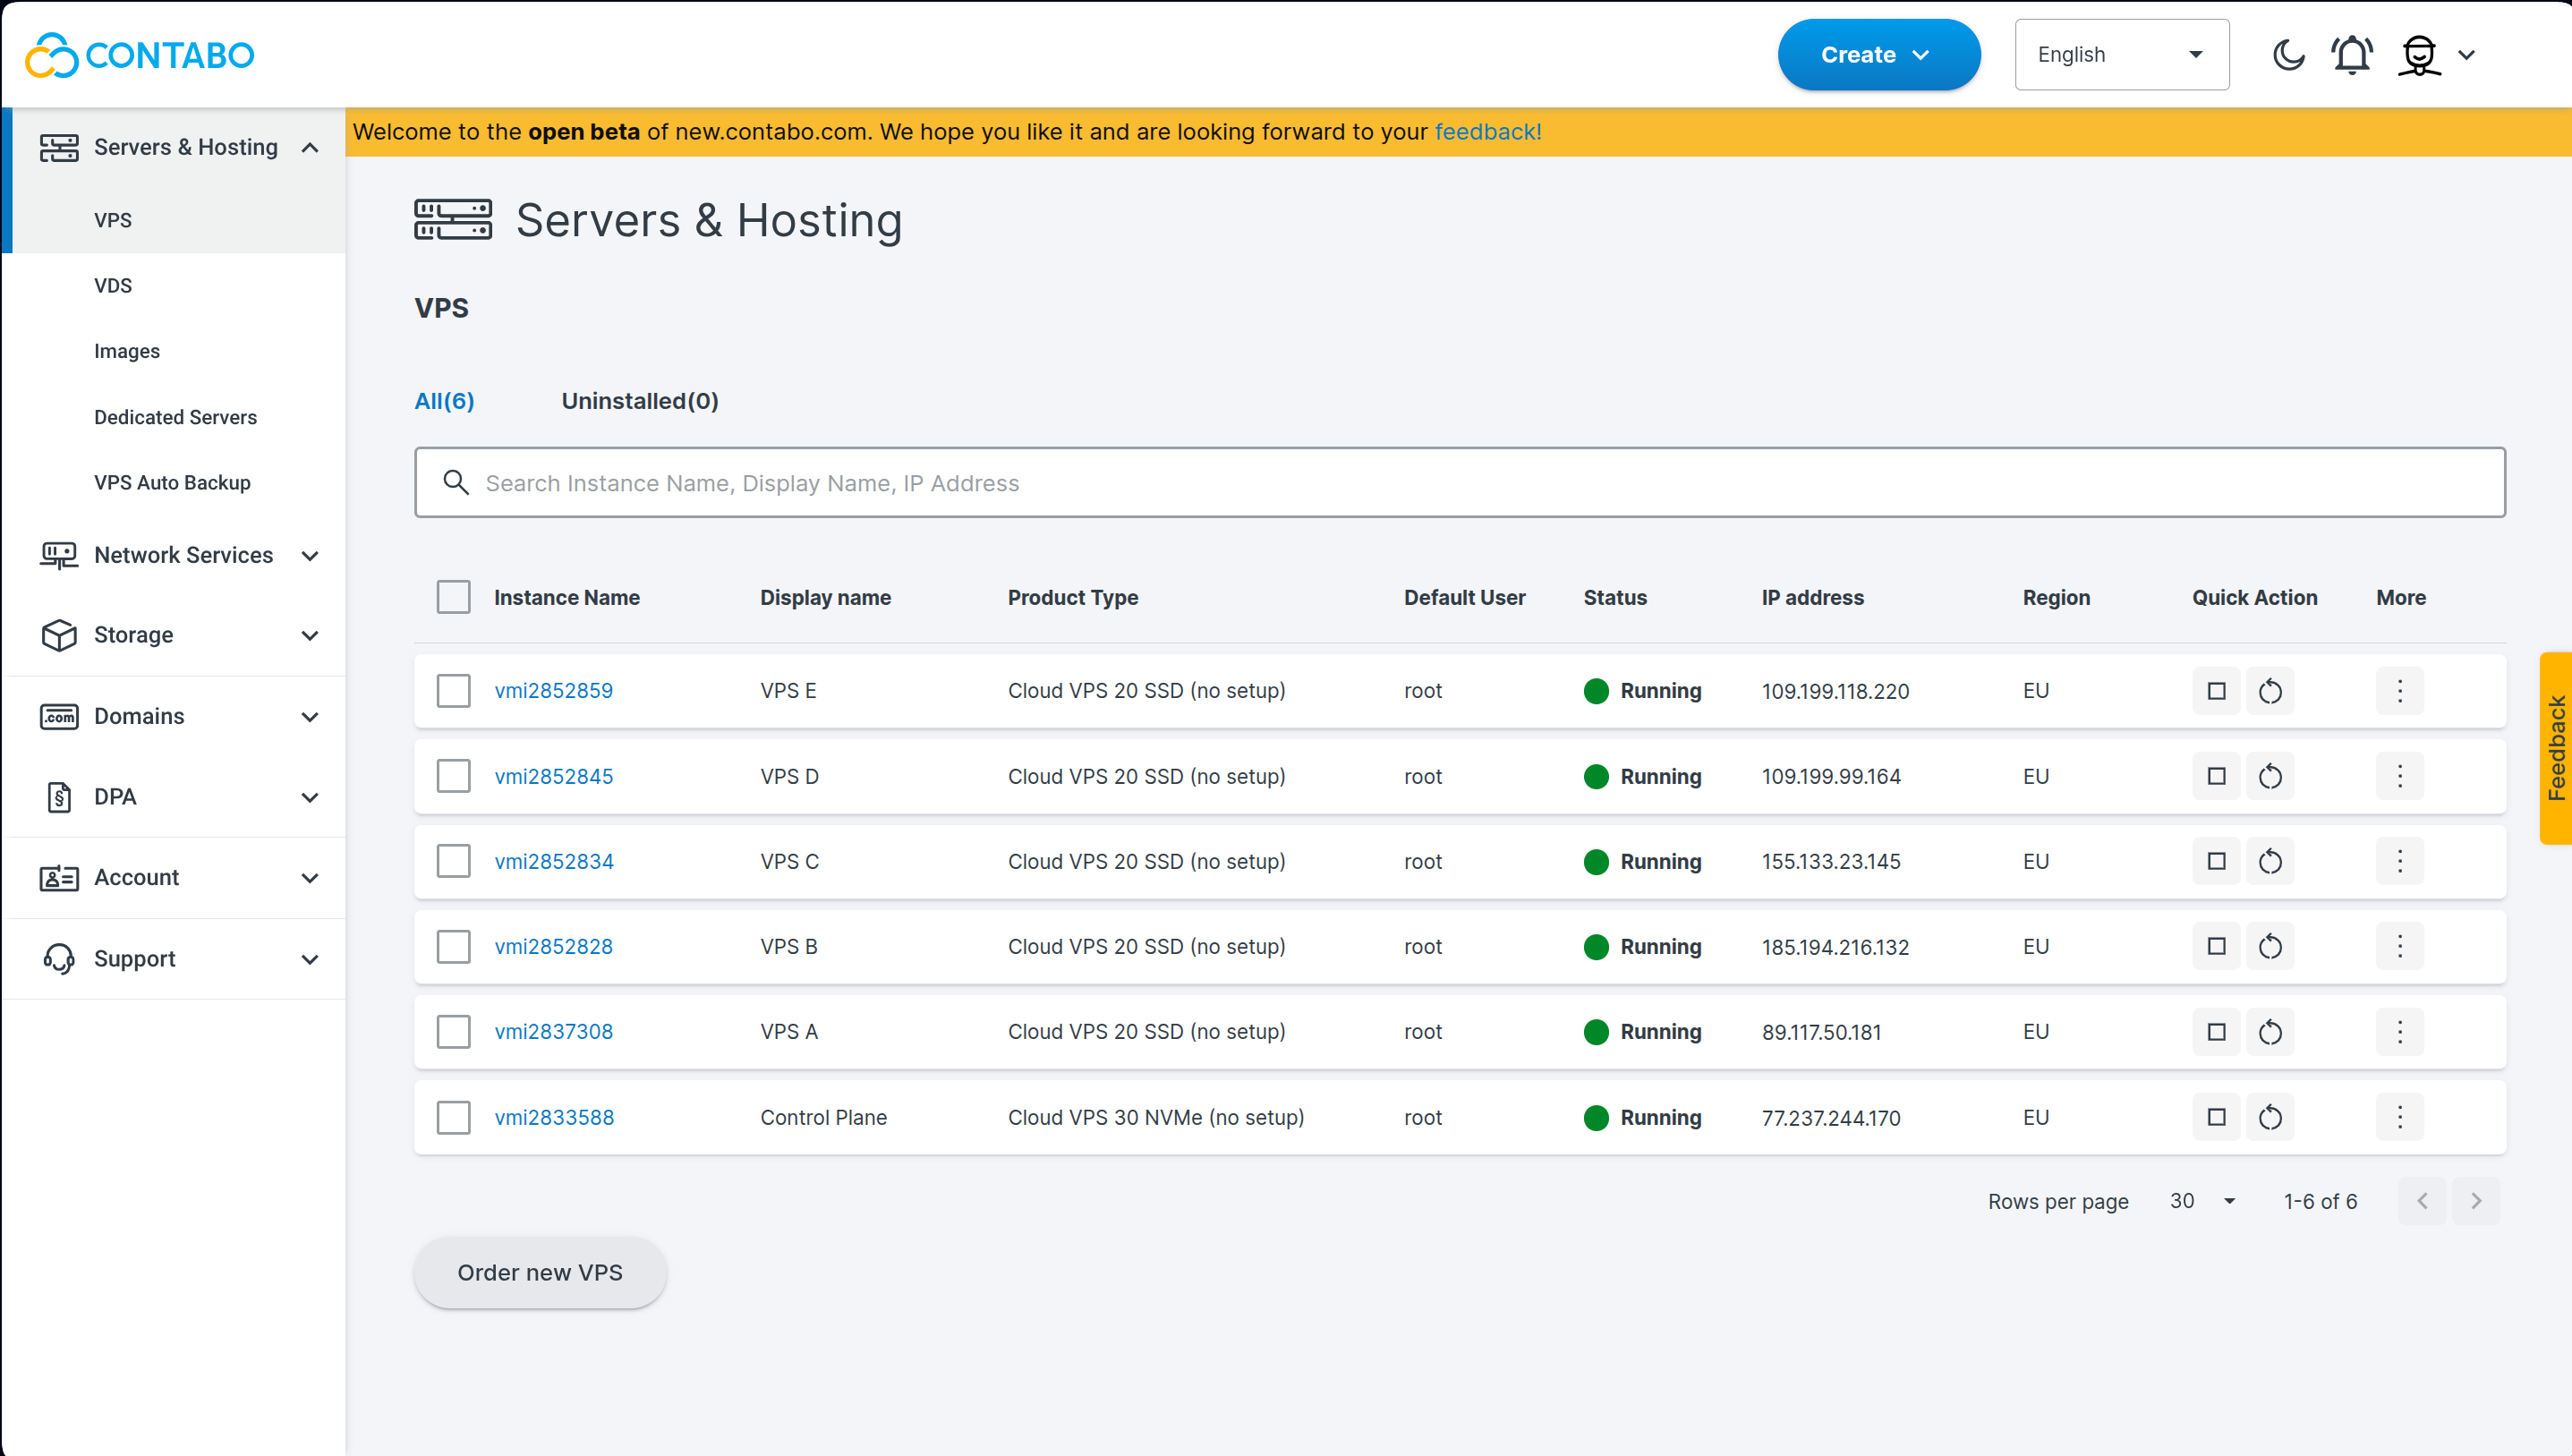
\includegraphics[width=1\textwidth]{images/vps-contabo.png}
    \caption{Daftar instance VPS Aktif di Provider Cloud (Contabo) yang terdiri dari 1 Control Plane dan 5 Worker Nodes.}
    \label{fig:vps_contabo}
\end{figure}

\begin{figure}[H]
    \centering
    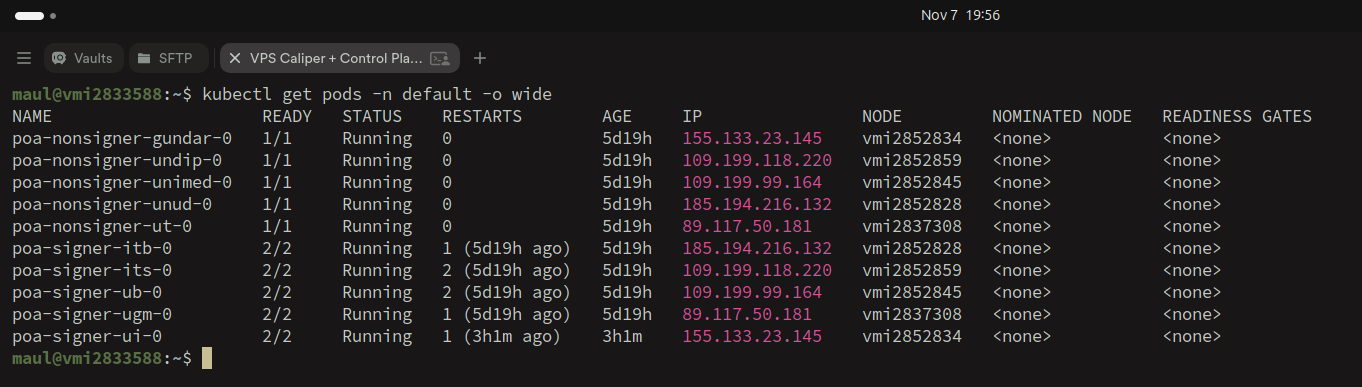
\includegraphics[width=1\textwidth]{images/kubectl-poa.png}
    \caption{Tampilan CLI \texttt{kubectl} yang menunjukkan status \textit{pods} container blockchain yang berjalan di dalam cluster Kubernetes.}
    \label{fig:kubectl_status}
\end{figure}

\clearpage
\subsection{Evolusi Topologi Jaringan (Ethstats)}
Dokumentasi ini menunjukkan perubahan topologi jaringan sesuai skenario pengujian (Skenario 1, 2, dan 3) yang dipantau melalui dashboard Ethstats.

\subsubsection{Proof of Authority (PoA)}
\begin{figure}[H]
    \centering
    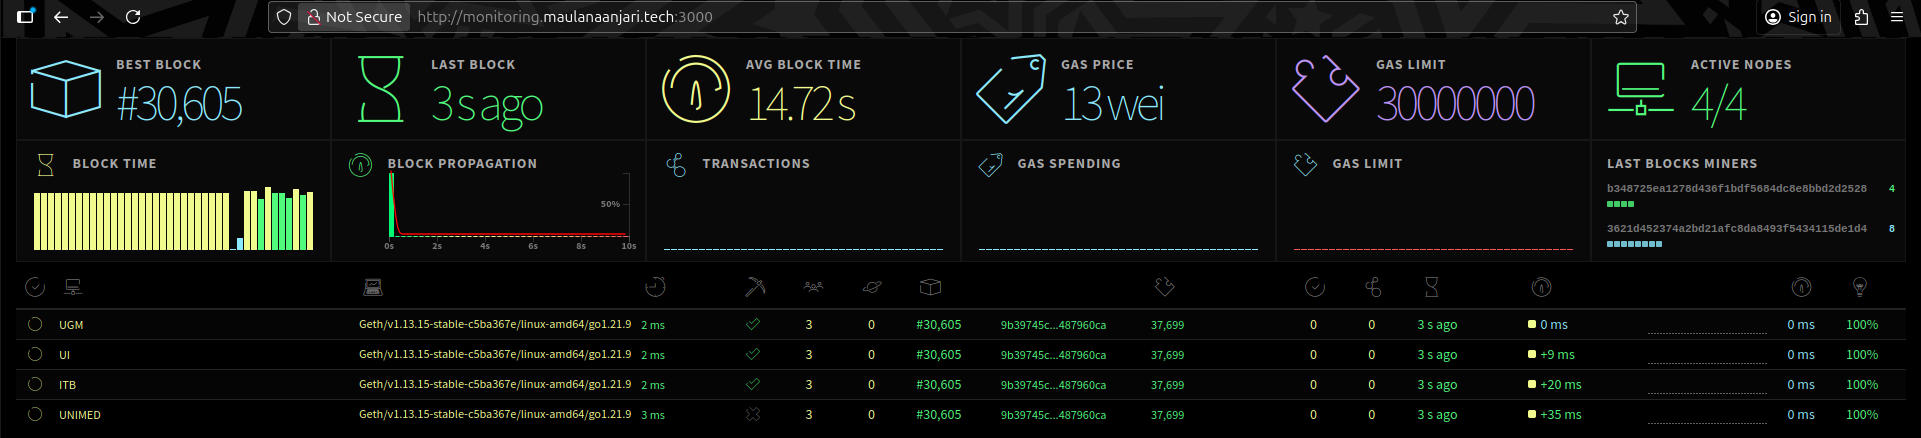
\includegraphics[width=1\textwidth]{images/ethstats-poa-3s-1ns.png}
    \caption{Ethstats PoA Skenario 1: 3 Signer + 1 Non-Signer (Total 4 Node).}
\end{figure}
\begin{figure}[H]
    \centering
    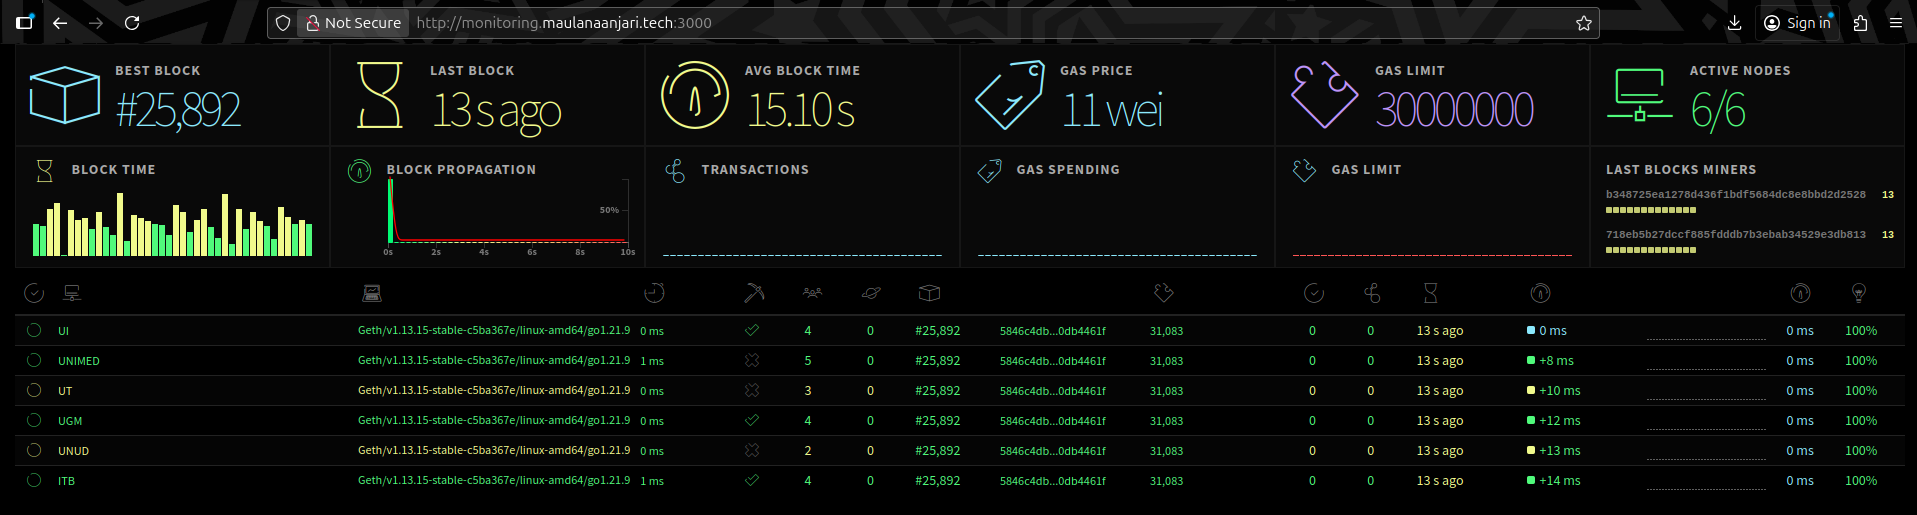
\includegraphics[width=1\textwidth]{images/ethstats-poa-3s-3ns.png}
    \caption{Ethstats PoA Skenario 2: 3 Signer + 3 Non-Signer (Total 6 Node).}
\end{figure}
\begin{figure}[H]
    \centering
    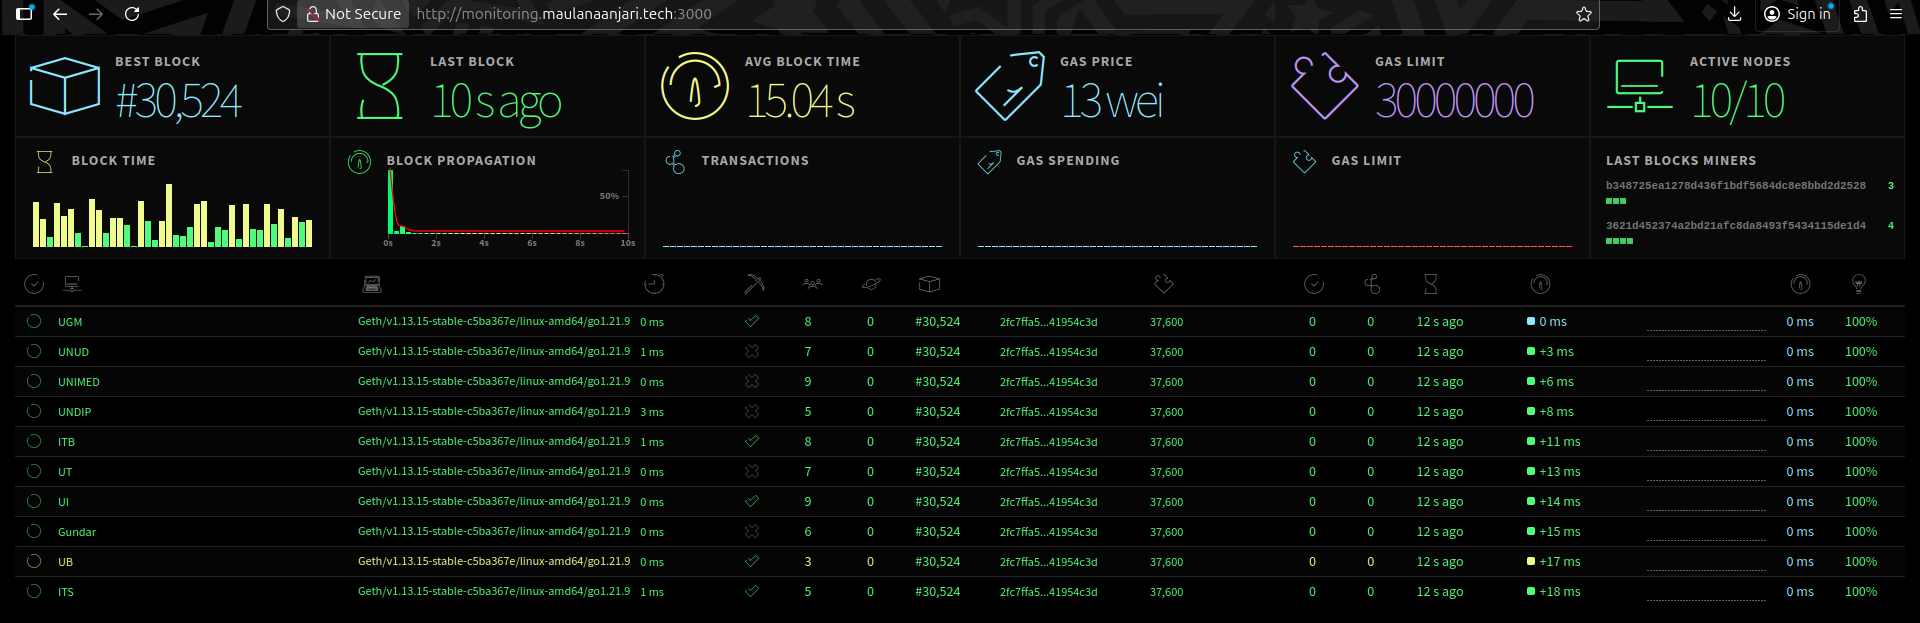
\includegraphics[width=1\textwidth]{images/ethstats-poa-5s-5ns.png}
    \caption{Ethstats PoA Skenario 3: 5 Signer + 5 Non-Signer (Total 10 Node).}
\end{figure}

\clearpage
\subsubsection{Proof of Stake (PoS)}
\begin{figure}[H]
    \centering
    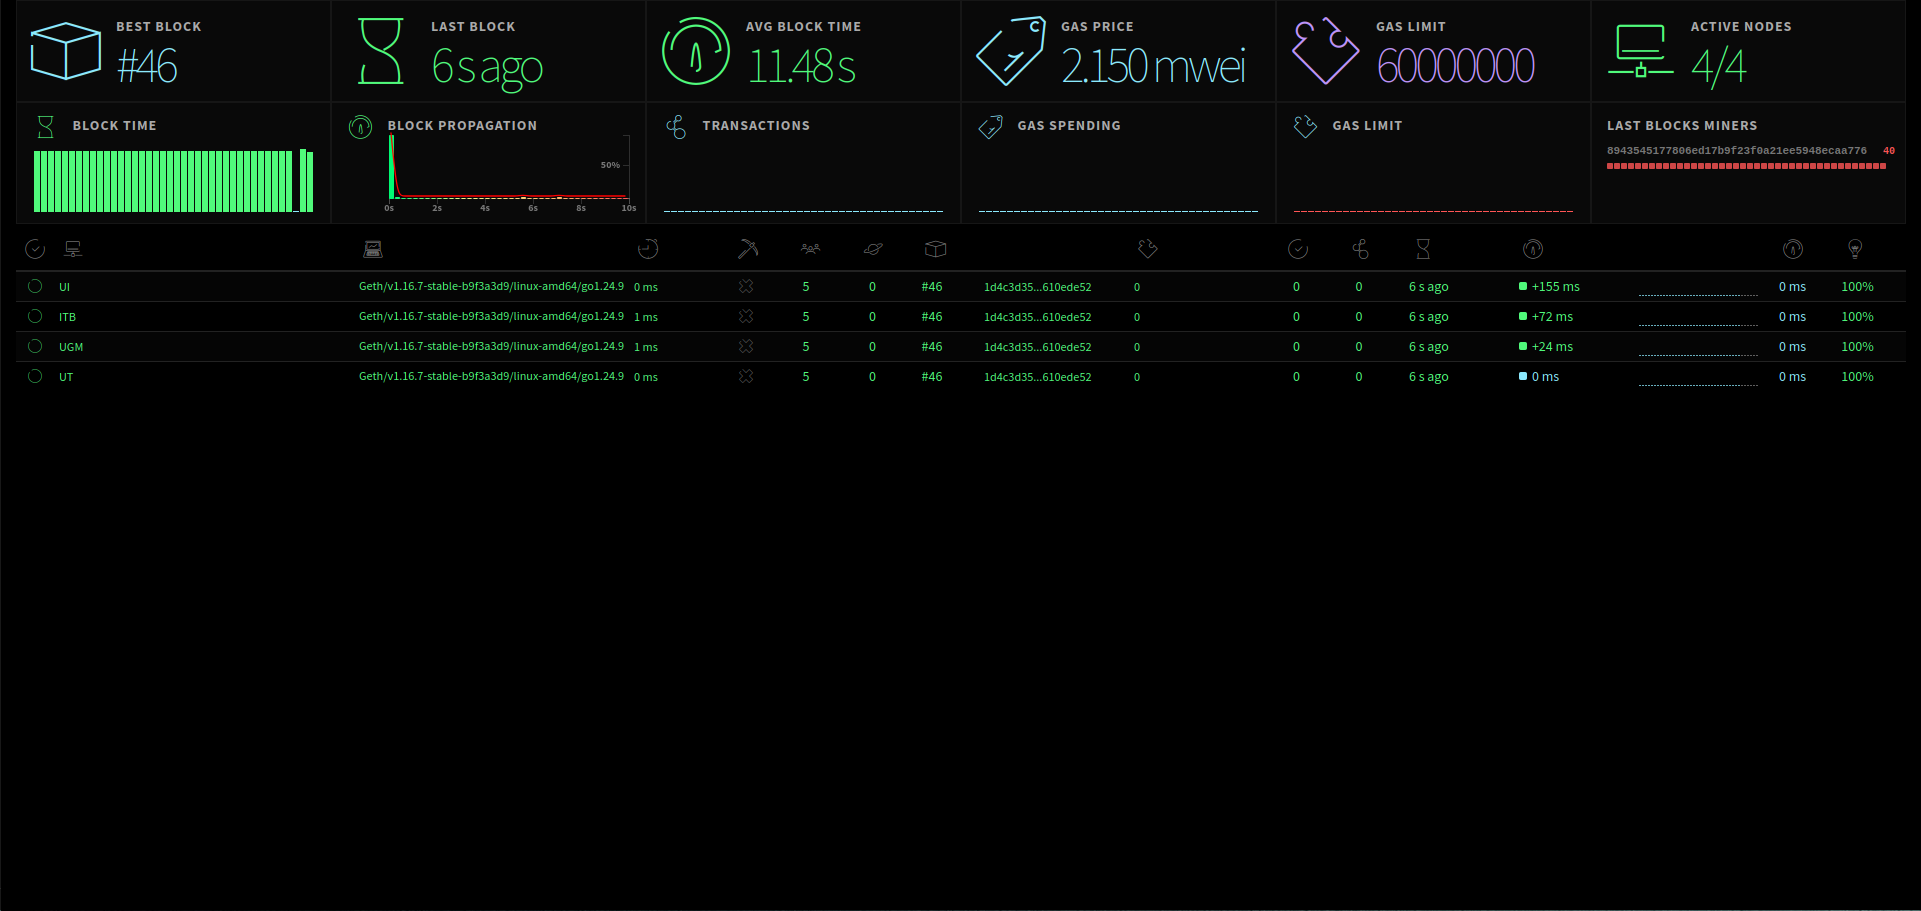
\includegraphics[width=1\textwidth]{images/ethstats-pos-3v-1nv.png}
    \caption{Ethstats PoS Skenario 1: 3 Validator + 1 Non-Validator (Total 4 Node).}
\end{figure}
\begin{figure}[H]
    \centering
    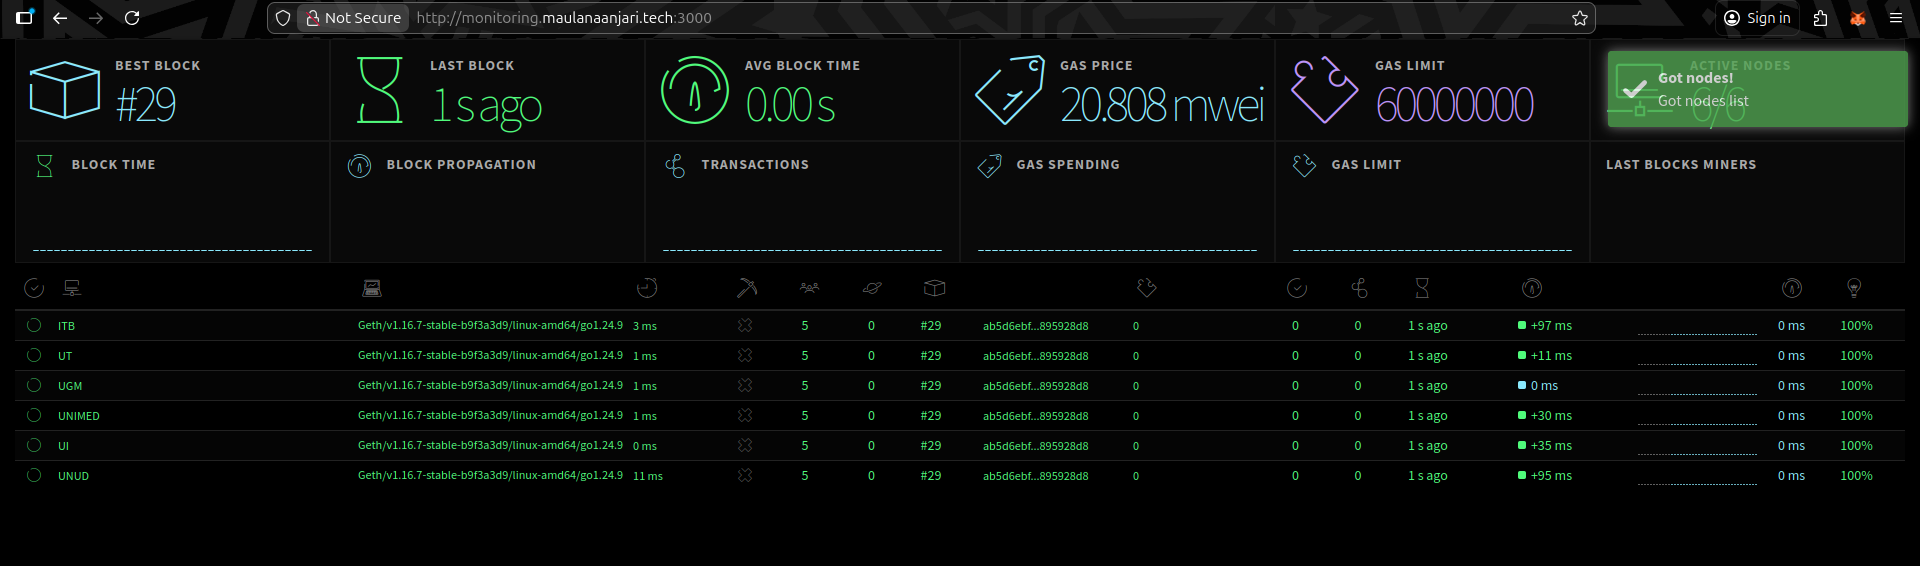
\includegraphics[width=1\textwidth]{images/ethstats-pos-3v-3nv.png}
    \caption{Ethstats PoS Skenario 2: 3 Validator + 3 Non-Validator (Total 6 Node).}
\end{figure}
\begin{figure}[H]
    \centering
    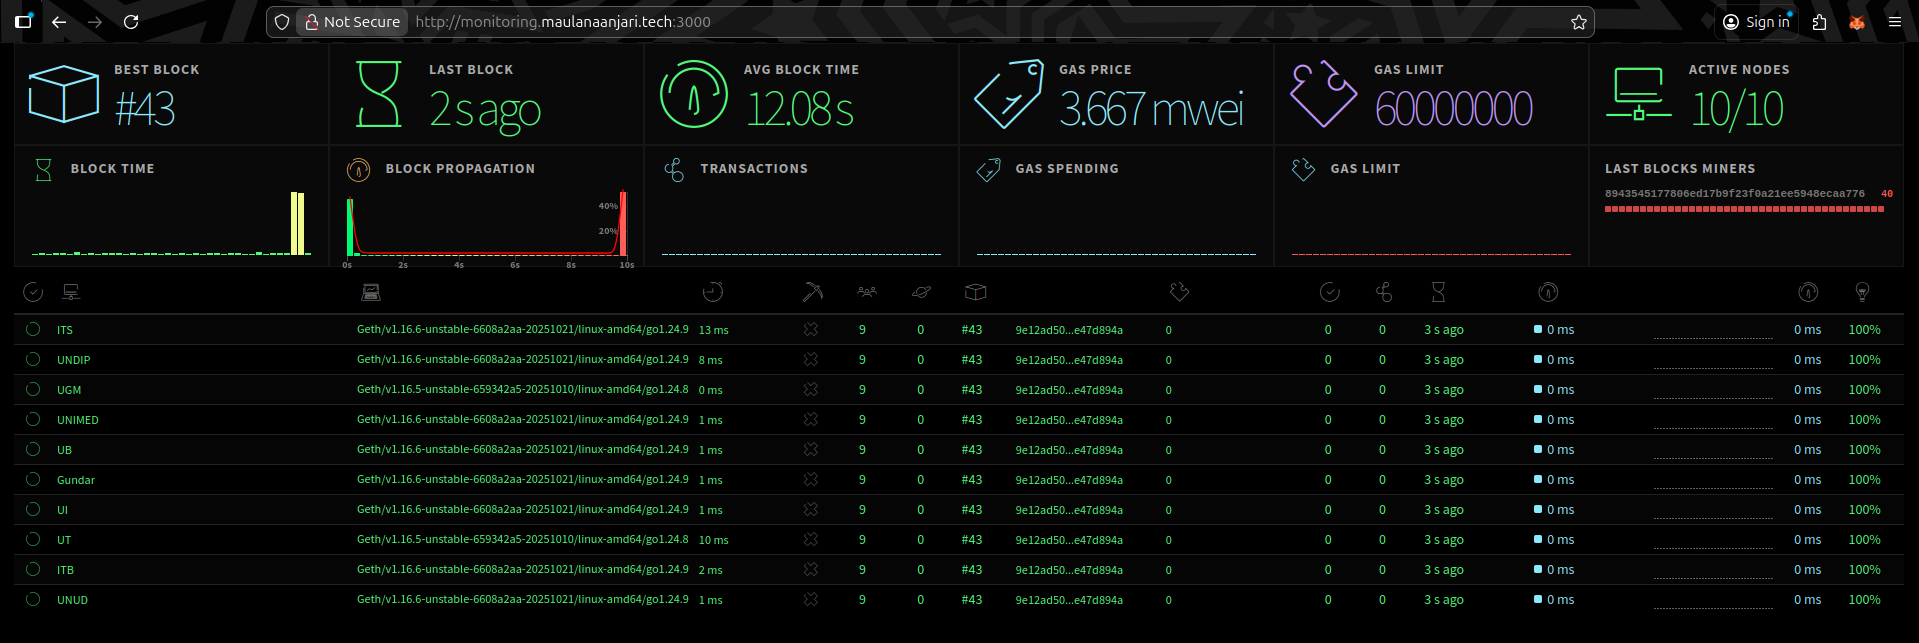
\includegraphics[width=1\textwidth]{images/ethstats-pos-5v-5nv.png}
    \caption{Ethstats PoS Skenario 3: 5 Validator + 5 Non-Validator (Total 10 Node).}
\end{figure}

\clearpage
\subsection{Status Konektivitas Monitoring (Prometheus)}
Halaman \textit{Targets} pada Prometheus yang memverifikasi bahwa seluruh \textit{exporter} data (Node Exporter, cAdvisor, Geth) terhubung dengan sukses (State: UP).

\begin{figure}[H]
    \centering
    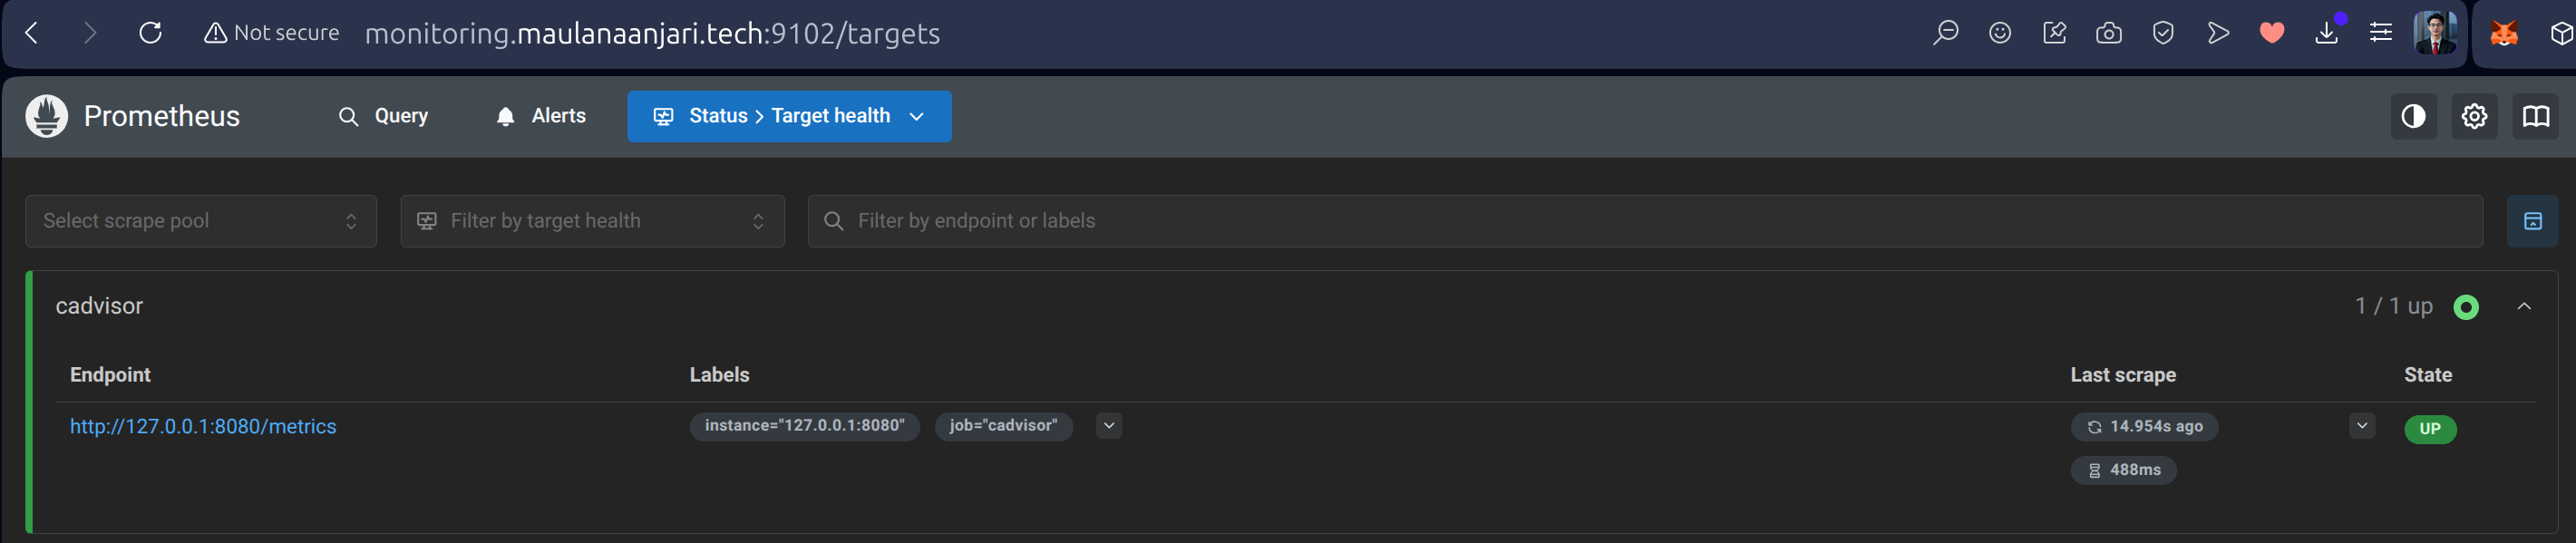
\includegraphics[width=1\textwidth]{images/prometheus-poa-all-connected-1.png}
    \caption{Status Target Prometheus (Bagian 1): Koneksi ke cAdvisor Container.}
\end{figure}
\begin{figure}[H]
    \centering
    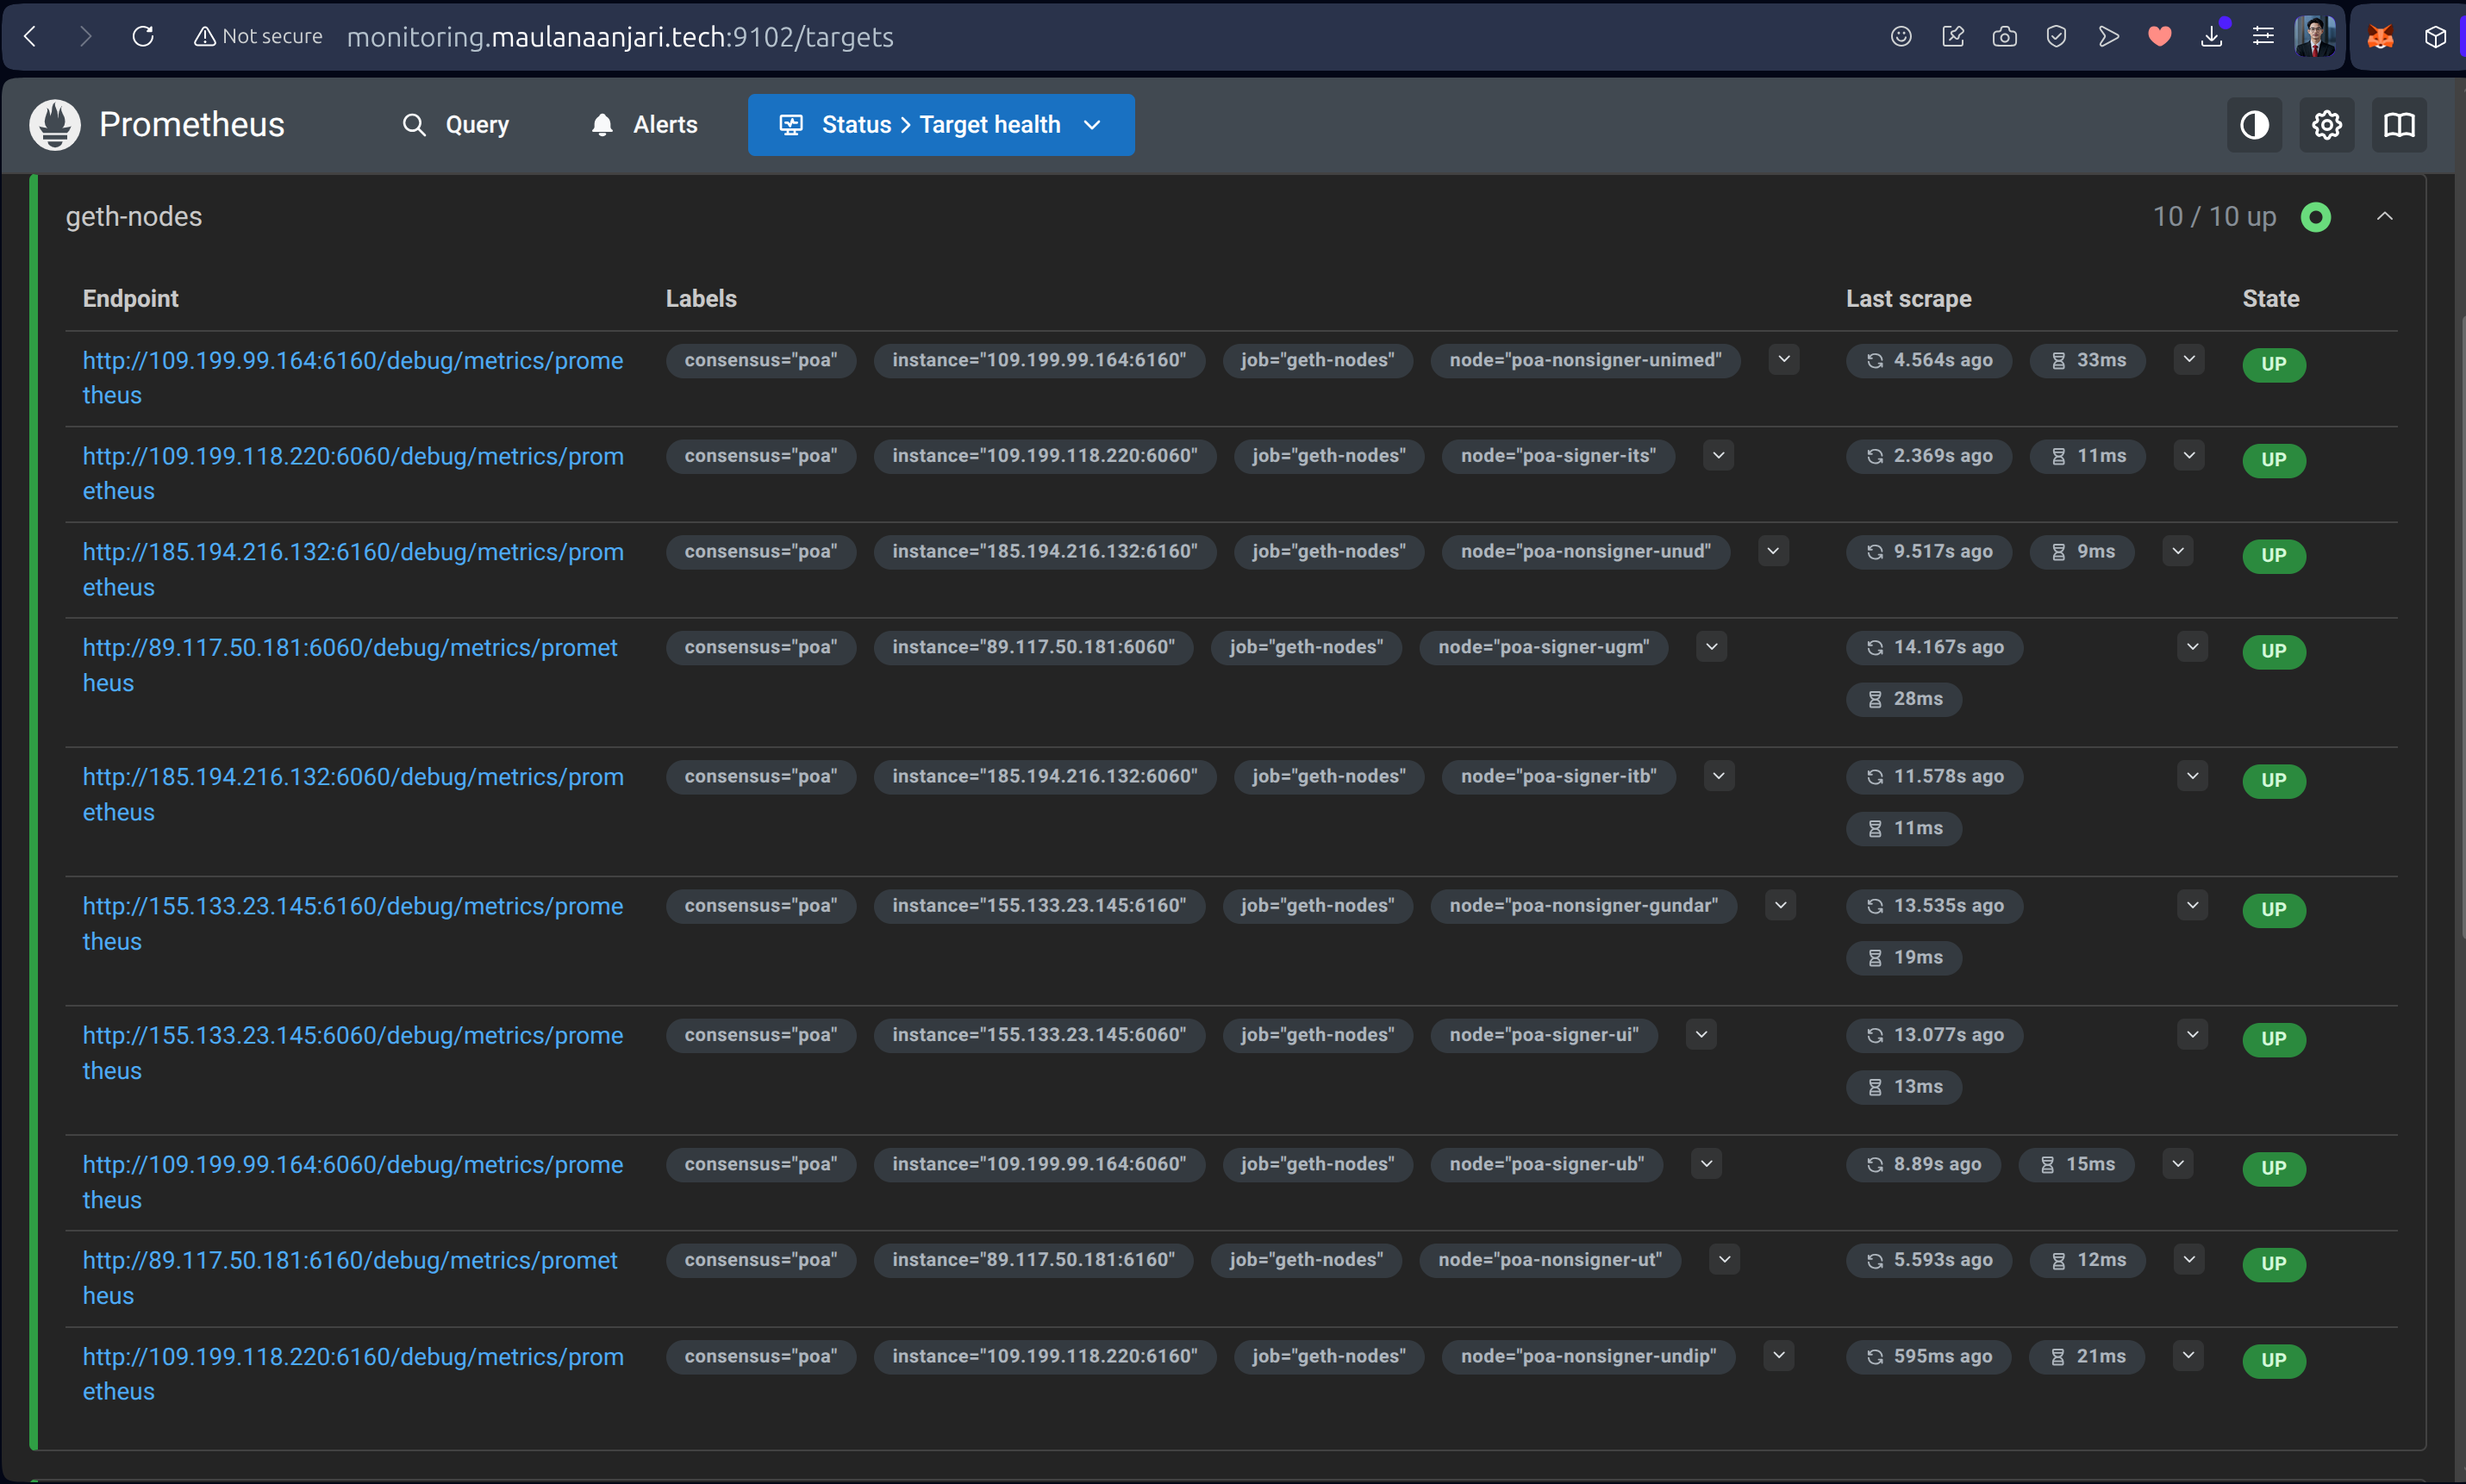
\includegraphics[width=1\textwidth]{images/prometheus-poa-all-connected-2.png}
    \caption{Status Target Prometheus (Bagian 2): Koneksi ke Geth Metrics.}
\end{figure}
\begin{figure}[H]
    \centering
    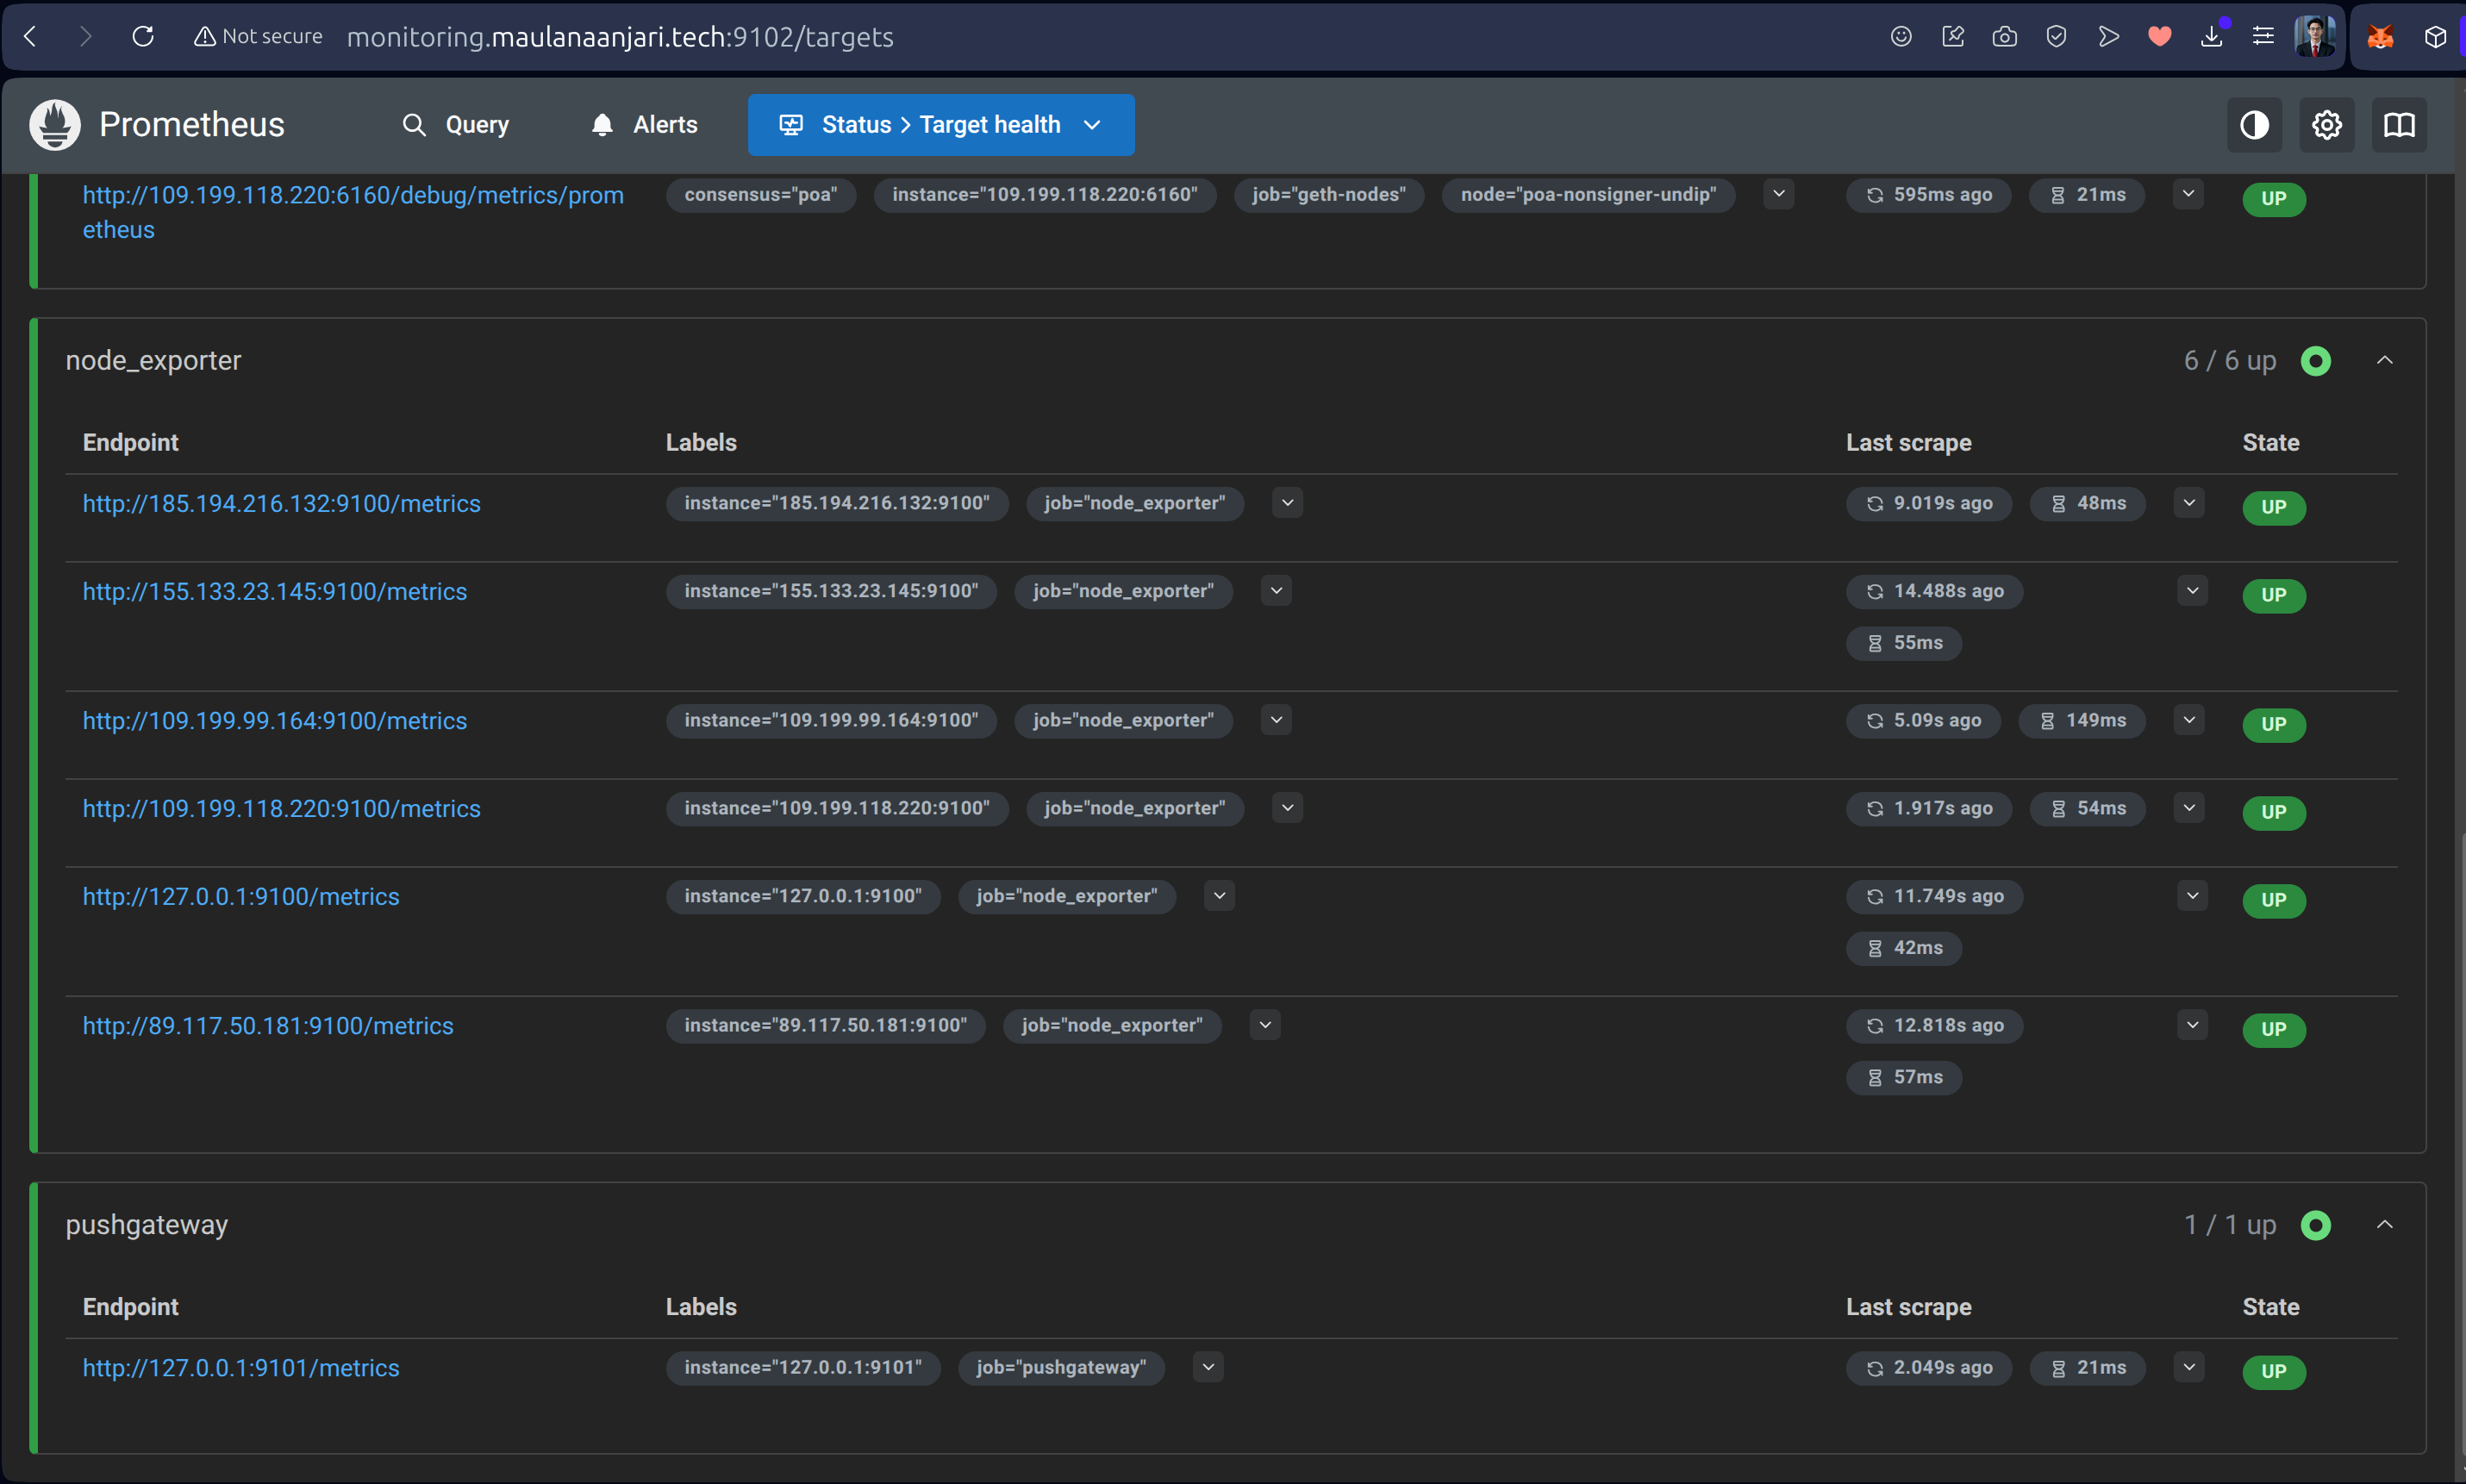
\includegraphics[width=1\textwidth]{images/prometheus-poa-all-connected-3.png}
    \caption{Status Target Prometheus (Bagian 3): Koneksi ke Node Exporter dan Pushgateway.}
\end{figure}

\clearpage
\subsection{Visualisasi Beban Sistem (Grafana)}
\begin{figure}[H]
    \centering
    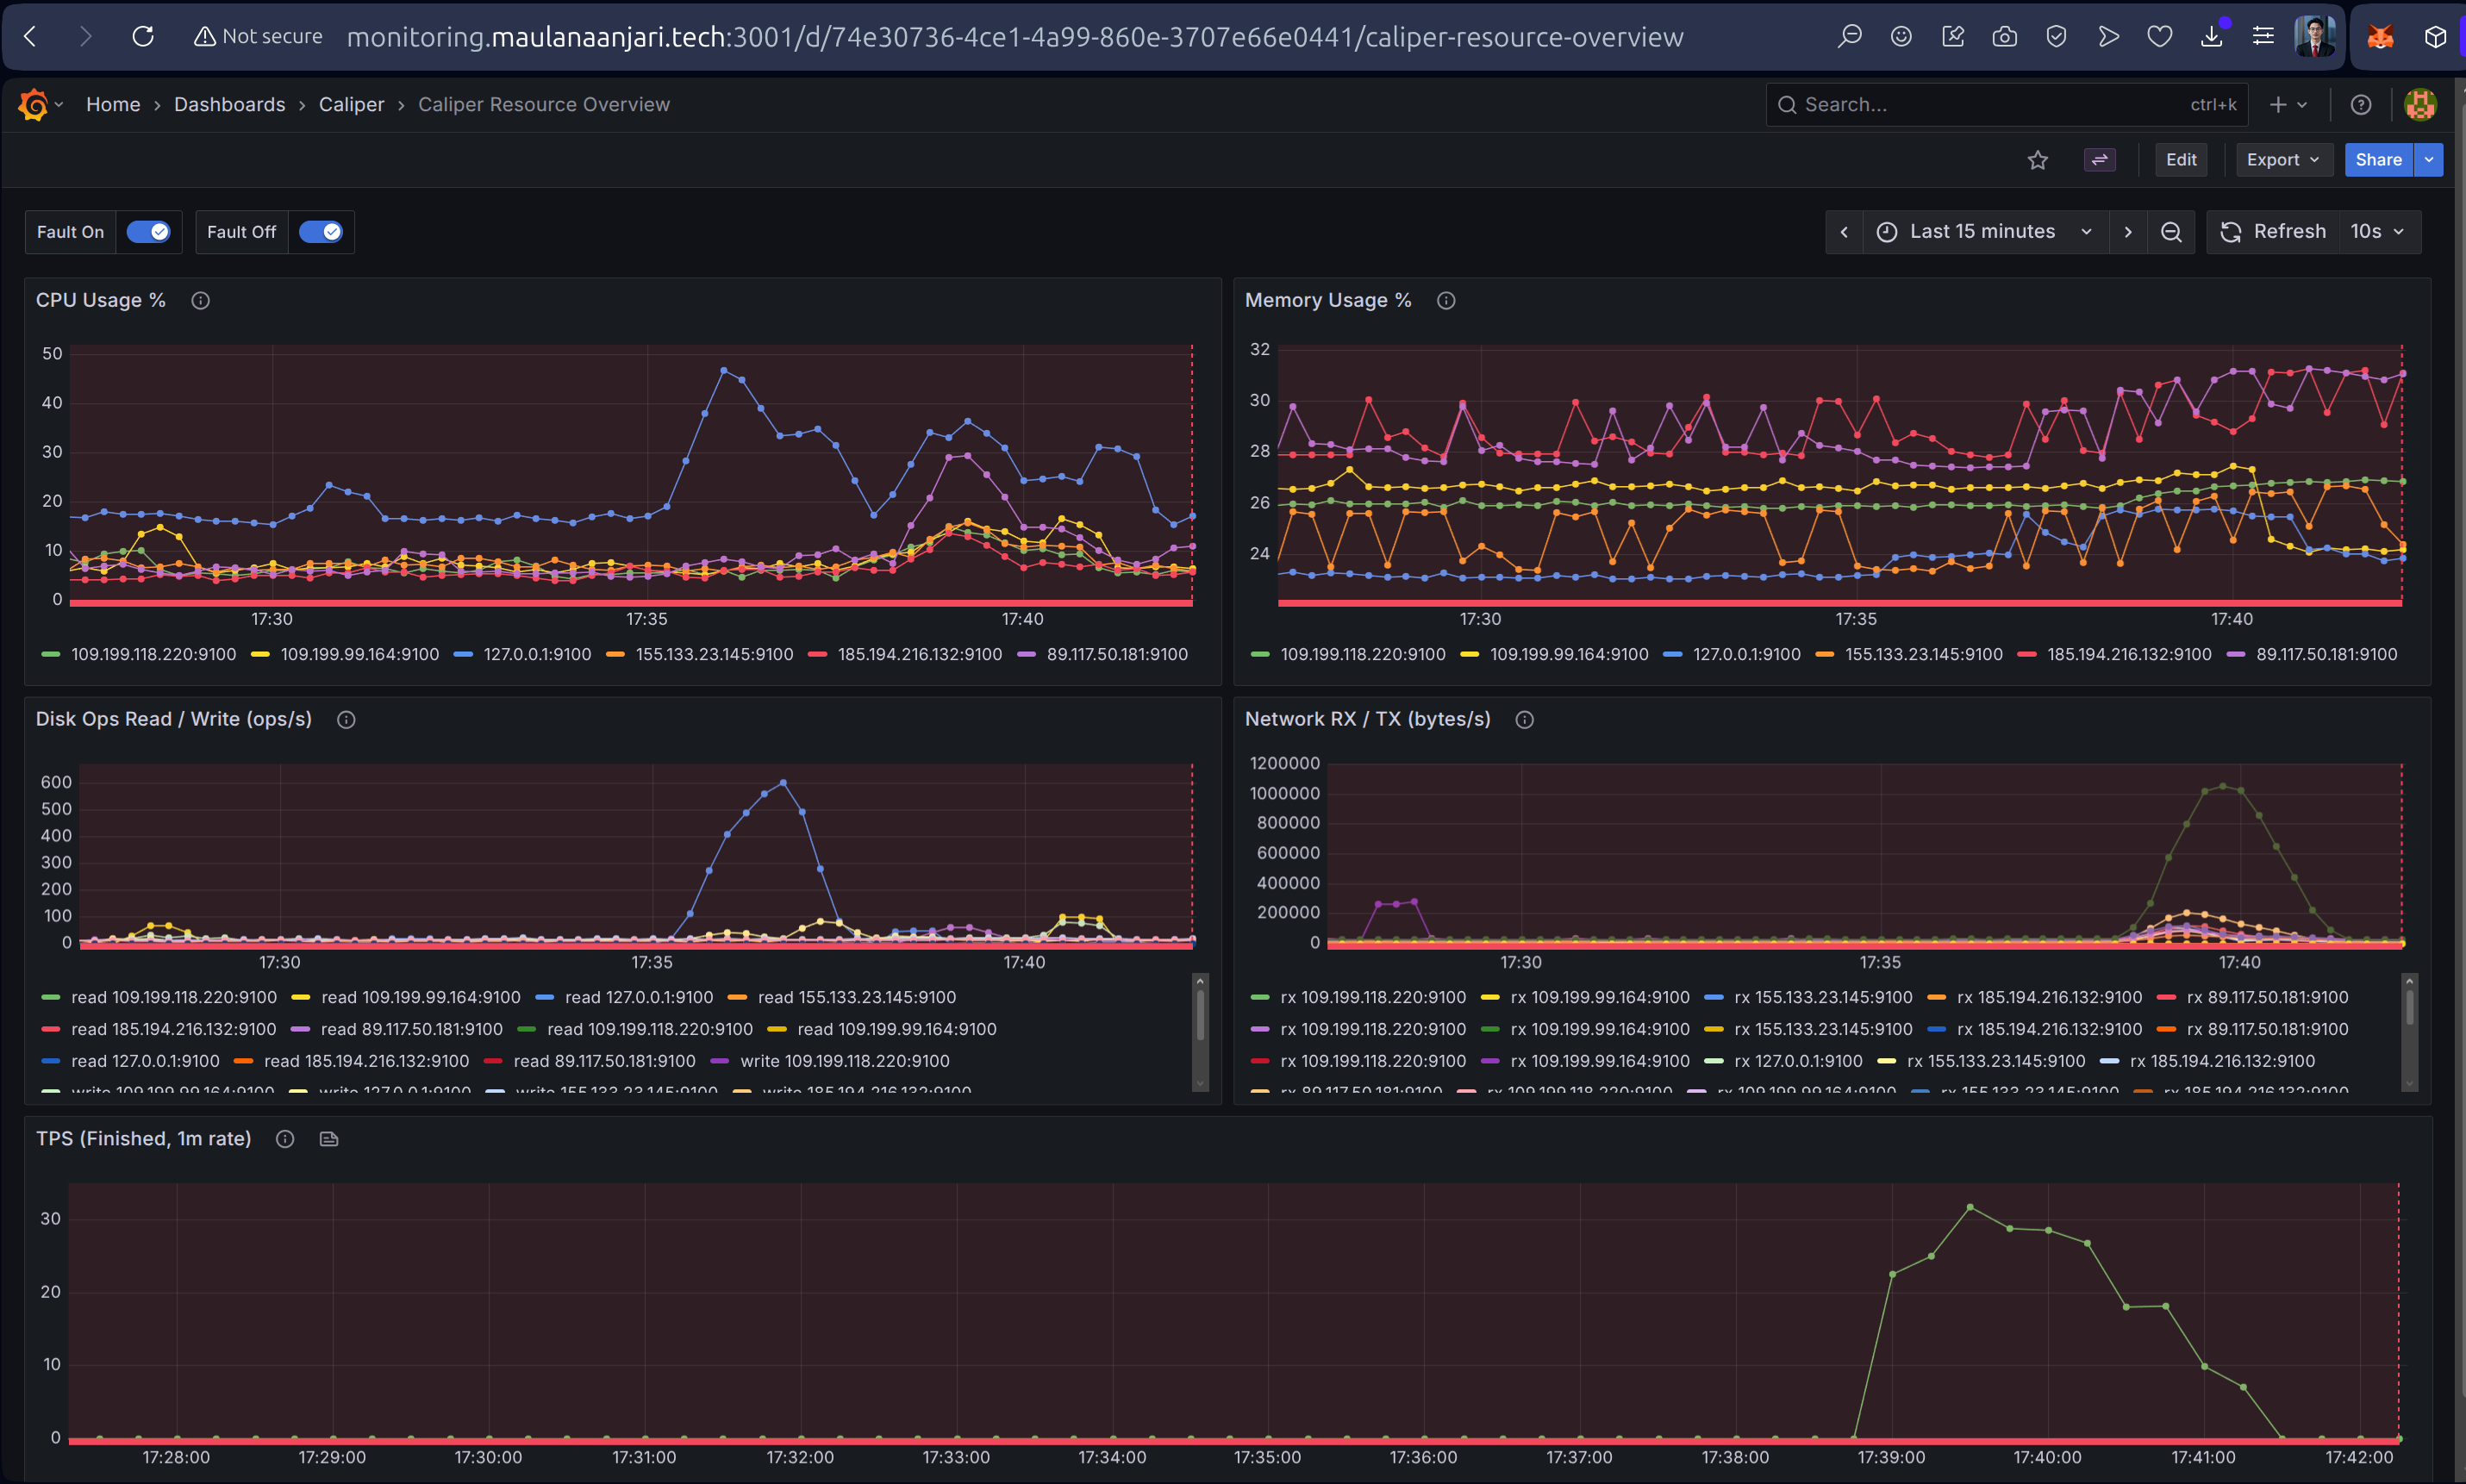
\includegraphics[width=1\textwidth]{images/grafana_resource_spike.png}
    \caption{Dashboard Grafana saat \textit{Load Test} 70 TPS. Terlihat korelasi antara panel TPS (bawah) yang aktif dengan lonjakan penggunaan CPU (kiri atas) dan Network (kanan tengah) pada seluruh node.}
    \label{fig:grafana_spike_full}
\end{figure}





%======================================

\end{document}
